
% Default to the notebook output style

    


% Inherit from the specified cell style.




    
\documentclass[11pt]{article}

    
    
    \usepackage[T1]{fontenc}
    % Nicer default font (+ math font) than Computer Modern for most use cases
    \usepackage{mathpazo}

    % Basic figure setup, for now with no caption control since it's done
    % automatically by Pandoc (which extracts ![](path) syntax from Markdown).
    \usepackage{graphicx}
    % We will generate all images so they have a width \maxwidth. This means
    % that they will get their normal width if they fit onto the page, but
    % are scaled down if they would overflow the margins.
    \makeatletter
    \def\maxwidth{\ifdim\Gin@nat@width>\linewidth\linewidth
    \else\Gin@nat@width\fi}
    \makeatother
    \let\Oldincludegraphics\includegraphics
    % Set max figure width to be 80% of text width, for now hardcoded.
    \renewcommand{\includegraphics}[1]{\Oldincludegraphics[width=.8\maxwidth]{#1}}
    % Ensure that by default, figures have no caption (until we provide a
    % proper Figure object with a Caption API and a way to capture that
    % in the conversion process - todo).
    \usepackage{caption}
    \DeclareCaptionLabelFormat{nolabel}{}
    \captionsetup{labelformat=nolabel}

    \usepackage{adjustbox} % Used to constrain images to a maximum size 
    \usepackage{xcolor} % Allow colors to be defined
    \usepackage{enumerate} % Needed for markdown enumerations to work
    \usepackage{geometry} % Used to adjust the document margins
    \usepackage{amsmath} % Equations
    \usepackage{amssymb} % Equations
    \usepackage{textcomp} % defines textquotesingle
    % Hack from http://tex.stackexchange.com/a/47451/13684:
    \AtBeginDocument{%
        \def\PYZsq{\textquotesingle}% Upright quotes in Pygmentized code
    }
    \usepackage{upquote} % Upright quotes for verbatim code
    \usepackage{eurosym} % defines \euro
    \usepackage[mathletters]{ucs} % Extended unicode (utf-8) support
    \usepackage[utf8x]{inputenc} % Allow utf-8 characters in the tex document
    \usepackage{fancyvrb} % verbatim replacement that allows latex
    \usepackage{grffile} % extends the file name processing of package graphics 
                         % to support a larger range 
    % The hyperref package gives us a pdf with properly built
    % internal navigation ('pdf bookmarks' for the table of contents,
    % internal cross-reference links, web links for URLs, etc.)
    \usepackage{hyperref}
    \usepackage{longtable} % longtable support required by pandoc >1.10
    \usepackage{booktabs}  % table support for pandoc > 1.12.2
    \usepackage[inline]{enumitem} % IRkernel/repr support (it uses the enumerate* environment)
    \usepackage[normalem]{ulem} % ulem is needed to support strikethroughs (\sout)
                                % normalem makes italics be italics, not underlines
    

    
    
    % Colors for the hyperref package
    \definecolor{urlcolor}{rgb}{0,.145,.698}
    \definecolor{linkcolor}{rgb}{.71,0.21,0.01}
    \definecolor{citecolor}{rgb}{.12,.54,.11}

    % ANSI colors
    \definecolor{ansi-black}{HTML}{3E424D}
    \definecolor{ansi-black-intense}{HTML}{282C36}
    \definecolor{ansi-red}{HTML}{E75C58}
    \definecolor{ansi-red-intense}{HTML}{B22B31}
    \definecolor{ansi-green}{HTML}{00A250}
    \definecolor{ansi-green-intense}{HTML}{007427}
    \definecolor{ansi-yellow}{HTML}{DDB62B}
    \definecolor{ansi-yellow-intense}{HTML}{B27D12}
    \definecolor{ansi-blue}{HTML}{208FFB}
    \definecolor{ansi-blue-intense}{HTML}{0065CA}
    \definecolor{ansi-magenta}{HTML}{D160C4}
    \definecolor{ansi-magenta-intense}{HTML}{A03196}
    \definecolor{ansi-cyan}{HTML}{60C6C8}
    \definecolor{ansi-cyan-intense}{HTML}{258F8F}
    \definecolor{ansi-white}{HTML}{C5C1B4}
    \definecolor{ansi-white-intense}{HTML}{A1A6B2}

    % commands and environments needed by pandoc snippets
    % extracted from the output of `pandoc -s`
    \providecommand{\tightlist}{%
      \setlength{\itemsep}{0pt}\setlength{\parskip}{0pt}}
    \DefineVerbatimEnvironment{Highlighting}{Verbatim}{commandchars=\\\{\}}
    % Add ',fontsize=\small' for more characters per line
    \newenvironment{Shaded}{}{}
    \newcommand{\KeywordTok}[1]{\textcolor[rgb]{0.00,0.44,0.13}{\textbf{{#1}}}}
    \newcommand{\DataTypeTok}[1]{\textcolor[rgb]{0.56,0.13,0.00}{{#1}}}
    \newcommand{\DecValTok}[1]{\textcolor[rgb]{0.25,0.63,0.44}{{#1}}}
    \newcommand{\BaseNTok}[1]{\textcolor[rgb]{0.25,0.63,0.44}{{#1}}}
    \newcommand{\FloatTok}[1]{\textcolor[rgb]{0.25,0.63,0.44}{{#1}}}
    \newcommand{\CharTok}[1]{\textcolor[rgb]{0.25,0.44,0.63}{{#1}}}
    \newcommand{\StringTok}[1]{\textcolor[rgb]{0.25,0.44,0.63}{{#1}}}
    \newcommand{\CommentTok}[1]{\textcolor[rgb]{0.38,0.63,0.69}{\textit{{#1}}}}
    \newcommand{\OtherTok}[1]{\textcolor[rgb]{0.00,0.44,0.13}{{#1}}}
    \newcommand{\AlertTok}[1]{\textcolor[rgb]{1.00,0.00,0.00}{\textbf{{#1}}}}
    \newcommand{\FunctionTok}[1]{\textcolor[rgb]{0.02,0.16,0.49}{{#1}}}
    \newcommand{\RegionMarkerTok}[1]{{#1}}
    \newcommand{\ErrorTok}[1]{\textcolor[rgb]{1.00,0.00,0.00}{\textbf{{#1}}}}
    \newcommand{\NormalTok}[1]{{#1}}
    
    % Additional commands for more recent versions of Pandoc
    \newcommand{\ConstantTok}[1]{\textcolor[rgb]{0.53,0.00,0.00}{{#1}}}
    \newcommand{\SpecialCharTok}[1]{\textcolor[rgb]{0.25,0.44,0.63}{{#1}}}
    \newcommand{\VerbatimStringTok}[1]{\textcolor[rgb]{0.25,0.44,0.63}{{#1}}}
    \newcommand{\SpecialStringTok}[1]{\textcolor[rgb]{0.73,0.40,0.53}{{#1}}}
    \newcommand{\ImportTok}[1]{{#1}}
    \newcommand{\DocumentationTok}[1]{\textcolor[rgb]{0.73,0.13,0.13}{\textit{{#1}}}}
    \newcommand{\AnnotationTok}[1]{\textcolor[rgb]{0.38,0.63,0.69}{\textbf{\textit{{#1}}}}}
    \newcommand{\CommentVarTok}[1]{\textcolor[rgb]{0.38,0.63,0.69}{\textbf{\textit{{#1}}}}}
    \newcommand{\VariableTok}[1]{\textcolor[rgb]{0.10,0.09,0.49}{{#1}}}
    \newcommand{\ControlFlowTok}[1]{\textcolor[rgb]{0.00,0.44,0.13}{\textbf{{#1}}}}
    \newcommand{\OperatorTok}[1]{\textcolor[rgb]{0.40,0.40,0.40}{{#1}}}
    \newcommand{\BuiltInTok}[1]{{#1}}
    \newcommand{\ExtensionTok}[1]{{#1}}
    \newcommand{\PreprocessorTok}[1]{\textcolor[rgb]{0.74,0.48,0.00}{{#1}}}
    \newcommand{\AttributeTok}[1]{\textcolor[rgb]{0.49,0.56,0.16}{{#1}}}
    \newcommand{\InformationTok}[1]{\textcolor[rgb]{0.38,0.63,0.69}{\textbf{\textit{{#1}}}}}
    \newcommand{\WarningTok}[1]{\textcolor[rgb]{0.38,0.63,0.69}{\textbf{\textit{{#1}}}}}
    
    
    % Define a nice break command that doesn't care if a line doesn't already
    % exist.
    \def\br{\hspace*{\fill} \\* }
    % Math Jax compatability definitions
    \def\gt{>}
    \def\lt{<}
    % Document parameters
    \title{@Lesson\_04\_DataStructure\_Binary\_Tree}
    
    
    

    % Pygments definitions
    
\makeatletter
\def\PY@reset{\let\PY@it=\relax \let\PY@bf=\relax%
    \let\PY@ul=\relax \let\PY@tc=\relax%
    \let\PY@bc=\relax \let\PY@ff=\relax}
\def\PY@tok#1{\csname PY@tok@#1\endcsname}
\def\PY@toks#1+{\ifx\relax#1\empty\else%
    \PY@tok{#1}\expandafter\PY@toks\fi}
\def\PY@do#1{\PY@bc{\PY@tc{\PY@ul{%
    \PY@it{\PY@bf{\PY@ff{#1}}}}}}}
\def\PY#1#2{\PY@reset\PY@toks#1+\relax+\PY@do{#2}}

\expandafter\def\csname PY@tok@w\endcsname{\def\PY@tc##1{\textcolor[rgb]{0.73,0.73,0.73}{##1}}}
\expandafter\def\csname PY@tok@c\endcsname{\let\PY@it=\textit\def\PY@tc##1{\textcolor[rgb]{0.25,0.50,0.50}{##1}}}
\expandafter\def\csname PY@tok@cp\endcsname{\def\PY@tc##1{\textcolor[rgb]{0.74,0.48,0.00}{##1}}}
\expandafter\def\csname PY@tok@k\endcsname{\let\PY@bf=\textbf\def\PY@tc##1{\textcolor[rgb]{0.00,0.50,0.00}{##1}}}
\expandafter\def\csname PY@tok@kp\endcsname{\def\PY@tc##1{\textcolor[rgb]{0.00,0.50,0.00}{##1}}}
\expandafter\def\csname PY@tok@kt\endcsname{\def\PY@tc##1{\textcolor[rgb]{0.69,0.00,0.25}{##1}}}
\expandafter\def\csname PY@tok@o\endcsname{\def\PY@tc##1{\textcolor[rgb]{0.40,0.40,0.40}{##1}}}
\expandafter\def\csname PY@tok@ow\endcsname{\let\PY@bf=\textbf\def\PY@tc##1{\textcolor[rgb]{0.67,0.13,1.00}{##1}}}
\expandafter\def\csname PY@tok@nb\endcsname{\def\PY@tc##1{\textcolor[rgb]{0.00,0.50,0.00}{##1}}}
\expandafter\def\csname PY@tok@nf\endcsname{\def\PY@tc##1{\textcolor[rgb]{0.00,0.00,1.00}{##1}}}
\expandafter\def\csname PY@tok@nc\endcsname{\let\PY@bf=\textbf\def\PY@tc##1{\textcolor[rgb]{0.00,0.00,1.00}{##1}}}
\expandafter\def\csname PY@tok@nn\endcsname{\let\PY@bf=\textbf\def\PY@tc##1{\textcolor[rgb]{0.00,0.00,1.00}{##1}}}
\expandafter\def\csname PY@tok@ne\endcsname{\let\PY@bf=\textbf\def\PY@tc##1{\textcolor[rgb]{0.82,0.25,0.23}{##1}}}
\expandafter\def\csname PY@tok@nv\endcsname{\def\PY@tc##1{\textcolor[rgb]{0.10,0.09,0.49}{##1}}}
\expandafter\def\csname PY@tok@no\endcsname{\def\PY@tc##1{\textcolor[rgb]{0.53,0.00,0.00}{##1}}}
\expandafter\def\csname PY@tok@nl\endcsname{\def\PY@tc##1{\textcolor[rgb]{0.63,0.63,0.00}{##1}}}
\expandafter\def\csname PY@tok@ni\endcsname{\let\PY@bf=\textbf\def\PY@tc##1{\textcolor[rgb]{0.60,0.60,0.60}{##1}}}
\expandafter\def\csname PY@tok@na\endcsname{\def\PY@tc##1{\textcolor[rgb]{0.49,0.56,0.16}{##1}}}
\expandafter\def\csname PY@tok@nt\endcsname{\let\PY@bf=\textbf\def\PY@tc##1{\textcolor[rgb]{0.00,0.50,0.00}{##1}}}
\expandafter\def\csname PY@tok@nd\endcsname{\def\PY@tc##1{\textcolor[rgb]{0.67,0.13,1.00}{##1}}}
\expandafter\def\csname PY@tok@s\endcsname{\def\PY@tc##1{\textcolor[rgb]{0.73,0.13,0.13}{##1}}}
\expandafter\def\csname PY@tok@sd\endcsname{\let\PY@it=\textit\def\PY@tc##1{\textcolor[rgb]{0.73,0.13,0.13}{##1}}}
\expandafter\def\csname PY@tok@si\endcsname{\let\PY@bf=\textbf\def\PY@tc##1{\textcolor[rgb]{0.73,0.40,0.53}{##1}}}
\expandafter\def\csname PY@tok@se\endcsname{\let\PY@bf=\textbf\def\PY@tc##1{\textcolor[rgb]{0.73,0.40,0.13}{##1}}}
\expandafter\def\csname PY@tok@sr\endcsname{\def\PY@tc##1{\textcolor[rgb]{0.73,0.40,0.53}{##1}}}
\expandafter\def\csname PY@tok@ss\endcsname{\def\PY@tc##1{\textcolor[rgb]{0.10,0.09,0.49}{##1}}}
\expandafter\def\csname PY@tok@sx\endcsname{\def\PY@tc##1{\textcolor[rgb]{0.00,0.50,0.00}{##1}}}
\expandafter\def\csname PY@tok@m\endcsname{\def\PY@tc##1{\textcolor[rgb]{0.40,0.40,0.40}{##1}}}
\expandafter\def\csname PY@tok@gh\endcsname{\let\PY@bf=\textbf\def\PY@tc##1{\textcolor[rgb]{0.00,0.00,0.50}{##1}}}
\expandafter\def\csname PY@tok@gu\endcsname{\let\PY@bf=\textbf\def\PY@tc##1{\textcolor[rgb]{0.50,0.00,0.50}{##1}}}
\expandafter\def\csname PY@tok@gd\endcsname{\def\PY@tc##1{\textcolor[rgb]{0.63,0.00,0.00}{##1}}}
\expandafter\def\csname PY@tok@gi\endcsname{\def\PY@tc##1{\textcolor[rgb]{0.00,0.63,0.00}{##1}}}
\expandafter\def\csname PY@tok@gr\endcsname{\def\PY@tc##1{\textcolor[rgb]{1.00,0.00,0.00}{##1}}}
\expandafter\def\csname PY@tok@ge\endcsname{\let\PY@it=\textit}
\expandafter\def\csname PY@tok@gs\endcsname{\let\PY@bf=\textbf}
\expandafter\def\csname PY@tok@gp\endcsname{\let\PY@bf=\textbf\def\PY@tc##1{\textcolor[rgb]{0.00,0.00,0.50}{##1}}}
\expandafter\def\csname PY@tok@go\endcsname{\def\PY@tc##1{\textcolor[rgb]{0.53,0.53,0.53}{##1}}}
\expandafter\def\csname PY@tok@gt\endcsname{\def\PY@tc##1{\textcolor[rgb]{0.00,0.27,0.87}{##1}}}
\expandafter\def\csname PY@tok@err\endcsname{\def\PY@bc##1{\setlength{\fboxsep}{0pt}\fcolorbox[rgb]{1.00,0.00,0.00}{1,1,1}{\strut ##1}}}
\expandafter\def\csname PY@tok@kc\endcsname{\let\PY@bf=\textbf\def\PY@tc##1{\textcolor[rgb]{0.00,0.50,0.00}{##1}}}
\expandafter\def\csname PY@tok@kd\endcsname{\let\PY@bf=\textbf\def\PY@tc##1{\textcolor[rgb]{0.00,0.50,0.00}{##1}}}
\expandafter\def\csname PY@tok@kn\endcsname{\let\PY@bf=\textbf\def\PY@tc##1{\textcolor[rgb]{0.00,0.50,0.00}{##1}}}
\expandafter\def\csname PY@tok@kr\endcsname{\let\PY@bf=\textbf\def\PY@tc##1{\textcolor[rgb]{0.00,0.50,0.00}{##1}}}
\expandafter\def\csname PY@tok@bp\endcsname{\def\PY@tc##1{\textcolor[rgb]{0.00,0.50,0.00}{##1}}}
\expandafter\def\csname PY@tok@fm\endcsname{\def\PY@tc##1{\textcolor[rgb]{0.00,0.00,1.00}{##1}}}
\expandafter\def\csname PY@tok@vc\endcsname{\def\PY@tc##1{\textcolor[rgb]{0.10,0.09,0.49}{##1}}}
\expandafter\def\csname PY@tok@vg\endcsname{\def\PY@tc##1{\textcolor[rgb]{0.10,0.09,0.49}{##1}}}
\expandafter\def\csname PY@tok@vi\endcsname{\def\PY@tc##1{\textcolor[rgb]{0.10,0.09,0.49}{##1}}}
\expandafter\def\csname PY@tok@vm\endcsname{\def\PY@tc##1{\textcolor[rgb]{0.10,0.09,0.49}{##1}}}
\expandafter\def\csname PY@tok@sa\endcsname{\def\PY@tc##1{\textcolor[rgb]{0.73,0.13,0.13}{##1}}}
\expandafter\def\csname PY@tok@sb\endcsname{\def\PY@tc##1{\textcolor[rgb]{0.73,0.13,0.13}{##1}}}
\expandafter\def\csname PY@tok@sc\endcsname{\def\PY@tc##1{\textcolor[rgb]{0.73,0.13,0.13}{##1}}}
\expandafter\def\csname PY@tok@dl\endcsname{\def\PY@tc##1{\textcolor[rgb]{0.73,0.13,0.13}{##1}}}
\expandafter\def\csname PY@tok@s2\endcsname{\def\PY@tc##1{\textcolor[rgb]{0.73,0.13,0.13}{##1}}}
\expandafter\def\csname PY@tok@sh\endcsname{\def\PY@tc##1{\textcolor[rgb]{0.73,0.13,0.13}{##1}}}
\expandafter\def\csname PY@tok@s1\endcsname{\def\PY@tc##1{\textcolor[rgb]{0.73,0.13,0.13}{##1}}}
\expandafter\def\csname PY@tok@mb\endcsname{\def\PY@tc##1{\textcolor[rgb]{0.40,0.40,0.40}{##1}}}
\expandafter\def\csname PY@tok@mf\endcsname{\def\PY@tc##1{\textcolor[rgb]{0.40,0.40,0.40}{##1}}}
\expandafter\def\csname PY@tok@mh\endcsname{\def\PY@tc##1{\textcolor[rgb]{0.40,0.40,0.40}{##1}}}
\expandafter\def\csname PY@tok@mi\endcsname{\def\PY@tc##1{\textcolor[rgb]{0.40,0.40,0.40}{##1}}}
\expandafter\def\csname PY@tok@il\endcsname{\def\PY@tc##1{\textcolor[rgb]{0.40,0.40,0.40}{##1}}}
\expandafter\def\csname PY@tok@mo\endcsname{\def\PY@tc##1{\textcolor[rgb]{0.40,0.40,0.40}{##1}}}
\expandafter\def\csname PY@tok@ch\endcsname{\let\PY@it=\textit\def\PY@tc##1{\textcolor[rgb]{0.25,0.50,0.50}{##1}}}
\expandafter\def\csname PY@tok@cm\endcsname{\let\PY@it=\textit\def\PY@tc##1{\textcolor[rgb]{0.25,0.50,0.50}{##1}}}
\expandafter\def\csname PY@tok@cpf\endcsname{\let\PY@it=\textit\def\PY@tc##1{\textcolor[rgb]{0.25,0.50,0.50}{##1}}}
\expandafter\def\csname PY@tok@c1\endcsname{\let\PY@it=\textit\def\PY@tc##1{\textcolor[rgb]{0.25,0.50,0.50}{##1}}}
\expandafter\def\csname PY@tok@cs\endcsname{\let\PY@it=\textit\def\PY@tc##1{\textcolor[rgb]{0.25,0.50,0.50}{##1}}}

\def\PYZbs{\char`\\}
\def\PYZus{\char`\_}
\def\PYZob{\char`\{}
\def\PYZcb{\char`\}}
\def\PYZca{\char`\^}
\def\PYZam{\char`\&}
\def\PYZlt{\char`\<}
\def\PYZgt{\char`\>}
\def\PYZsh{\char`\#}
\def\PYZpc{\char`\%}
\def\PYZdl{\char`\$}
\def\PYZhy{\char`\-}
\def\PYZsq{\char`\'}
\def\PYZdq{\char`\"}
\def\PYZti{\char`\~}
% for compatibility with earlier versions
\def\PYZat{@}
\def\PYZlb{[}
\def\PYZrb{]}
\makeatother


    % Exact colors from NB
    \definecolor{incolor}{rgb}{0.0, 0.0, 0.5}
    \definecolor{outcolor}{rgb}{0.545, 0.0, 0.0}



    
    % Prevent overflowing lines due to hard-to-break entities
    \sloppy 
    % Setup hyperref package
    \hypersetup{
      breaklinks=true,  % so long urls are correctly broken across lines
      colorlinks=true,
      urlcolor=urlcolor,
      linkcolor=linkcolor,
      citecolor=citecolor,
      }
    % Slightly bigger margins than the latex defaults
    
    \geometry{verbose,tmargin=1in,bmargin=1in,lmargin=1in,rmargin=1in}
    
    

    \begin{document}
    
    
    \maketitle
    
    

    
    \subsection{\# Lesson 4: DATA STRUCTURE -\/- Binary
Tree}\label{lesson-4-data-structure----binary-tree}

In this lesson, we will cover the following parts: * 4.1: Lecture Note
-\/- Binary Tree * 4.2: Lecture Note -\/- Binary Search Tree * 4.3:
Lecture Note -\/- Advanced Tree * 4.4: Leetcode Training (Basic) * 4.5:
Leetcode Practice (Advanced)

{[}This topic is very basic and serves as building blocks for advanced
data structures and models. You should be familiar with these concepts
and problem-solving skills.{]}

     CRITICAL POINTS OF RECRUSION PROBLEMS

\begin{enumerate}
\def\labelenumi{\arabic{enumi}.}
\tightlist
\item
  How do you divide the problem into smaller ones?\\
  Ans:\\
\item
  What is the smallest problem -\/- base case condition?\\
  Ans: leaf node or next of leaf node
\item
  What to get from your children?\\
  Ans:
\item
  What to do in the current stage?\\
  Ans:
\item
  What to return to your parent?\\
  Ans:
\end{enumerate}

 信息传递:从上往下传加参数(Use extra prameters to pass info from the
top down), 从下往上传用返回(Use extra return to pass info from the
bottom up) 

    \subsubsection{重点题型(for
review)}\label{ux91cdux70b9ux9898ux578bfor-review}

独孤九剑 ------
破枪式:碰到二叉树的问题,就想想整棵树在该问题上的结果和左右儿子在该问题上的结果之间的联系是什么

\textbf{Binary Tree} 1.
\href{http://www.jiuzhang.com/solutions/maximum-depth-of-binary-tree/}{Maximum
Depth of Binary Tree} 2.
\href{https://www.jiuzhang.com/solutions/binary-tree-paths/}{Binary Tree
Paths} 3.
\href{http://www.jiuzhang.com/solutions/minimum-subtree/}{Minimum
Subtree} 4.
\href{http://www.jiuzhang.com/solutions/balanced-binary-tree/}{Balanced
Binary Tree} 5.
\href{http://www.jiuzhang.com/solutions/subtree-with-maximum-average/}{Subtree
with Maximum Average} 6.
\href{http://www.jiuzhang.com/solutions/flatten-binary-tree-to-linked-list/}{Flattern
Binary Tree to Linked List} 7.
\href{http://www.jiuzhang.com/solutions/lowest-common-ancestor/}{Lowest
Common Ancestor} Lowest Common Ancestor ii Lowest Common Ancestor iii 8.
\href{http://www.jiuzhang.com/solutions/binary-tree-longest-consecutive-sequence/}{Binary
Tree Longest Consecutive Sequence} Binary Tree Longest Consecutive
Sequence ii Binary Tree Longest Consecutive Sequence iii 9.
\href{http://www.lintcode.com/problem/binary-tree-path-sum/}{Binary Tree
Path Sum i}
\href{http://www.lintcode.com/problem/binary-tree-path-sum-ii/}{Binary
Tree Path Sum ii}
\href{http://www.lintcode.com/problem/binary-tree-path-sum-iii/}{Binary
Tree Path Sum iii}

\textbf{Binary Search Tree} 1.
\href{http://www.jiuzhang.com/solutions/validate-binary-search-tree/}{Validate
Binary Search Tree} 2.
\href{http://www.jiuzhang.com/solutions/convert-binary-search-tree-to-doubly-linked-list/}{Convert
Binary Search Tree to Doubly Linked List} 3.
\href{http://www.jiuzhang.com/solutions/binary-search-tree-iterator}{Binary
Search Tree Iterator} 4.
\href{http://www.jiuzhang.com/solutions/inorder-successor-in-binary-search-tree/}{In-order
Successor in Binary Search Tree} 5.
\href{http://www.lintcode.com/problem/search-range-in-binary-search-tree/}{Search
Range in Binary Search Tree} 6.
\href{http://www.lintcode.com/problem/insert-node-in-a-binary-search-tree/}{Insert
Node in a Binary Search Tree} 7.
\href{http://www.mathcs.emory.edu/~cheung/Courses/171/Syllabus/9-BinTree/BST-delete.html}{Remove
Node in a Binary Search Tree}

    \subsection{4.1 Lecture Note -\/- Binary
Tree}\label{lecture-note----binary-tree}

\subsubsection{4.1.1 Definition}\label{definition}

\paragraph{Tree}\label{tree}

In computer science, a tree is a widely used abstract data type (ADT)
--- or data structure implementing this ADT --- that simulates a
hierarchical tree structure, with a root value and subtrees of children
with a parent node, represented as a set of linked nodes.

{[}wiki{]}(https://en.wikipedia.org/wiki/Tree\_(data\_structure\%29)

\begin{figure}
\centering
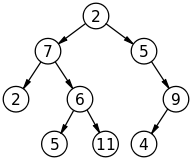
\includegraphics{source/lesson6_binarytree_btexample.png}
\caption{Tree Example}
\end{figure}

By definition, a tree is a data structure made up of nodes or vertices
and edges without having any cycle. The tree with no nodes is called the
null or empty tree. A tree that is not empty consists of a root node and
potentially many levels of additional nodes that form a hierarchy.

\begin{figure}
\centering
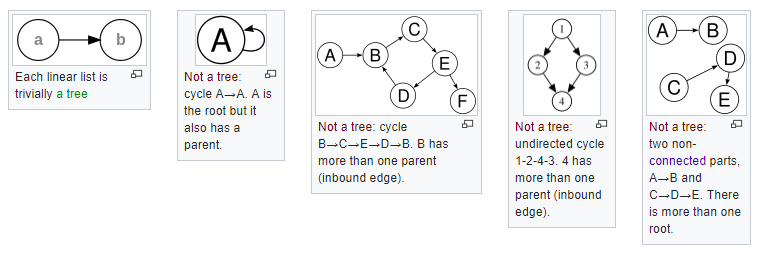
\includegraphics{source/lesson6_binarytree_treeexample.png}
\caption{Tree Example}
\end{figure}

\paragraph{Binary Tree}\label{binary-tree}

\href{https://en.wikipedia.org/wiki/Binary_tree}{wiki}

In computer science, a binary tree is a tree data structure in which
each node has at most two children, which are referred to as the left
child and the right child. A recursive definition using just set theory
notions is that a (non-empty) binary tree is a tuple (L, S, R), where L
and R are binary trees or the empty set and S is a singleton set.

Example:

\begin{verbatim}
                10 == root
               /  \
              5    15
             / \   / \
            2  7  12 20     <-- all leaf node's level == 3
           / \
        None None  
\end{verbatim}

How to define a tree class?

    \begin{Verbatim}[commandchars=\\\{\}]
{\color{incolor}In [{\color{incolor}76}]:} \PY{k}{class} \PY{n+nc}{TreeNode}\PY{p}{:}
             \PY{k}{def} \PY{n+nf}{\PYZus{}\PYZus{}init\PYZus{}\PYZus{}}\PY{p}{(}\PY{n+nb+bp}{self}\PY{p}{,} \PY{n}{x}\PY{p}{)}\PY{p}{:}
                 \PY{n+nb+bp}{self}\PY{o}{.}\PY{n}{val} \PY{o}{=} \PY{n}{x}
                 \PY{n+nb+bp}{self}\PY{o}{.}\PY{n}{left} \PY{o}{=} \PY{k+kc}{None}
                 \PY{n+nb+bp}{self}\PY{o}{.}\PY{n}{right} \PY{o}{=} \PY{k+kc}{None}
\end{Verbatim}


    \subsubsection{4.1.2 Tree Traversal}\label{tree-traversal}

\href{https://en.wikipedia.org/wiki/Tree_traversal}{Wiki\_TreeTraversal}
In computer science, tree traversal (also known as tree search) is a
form of graph traversal and refers to the process of visiting (checking
and/or updating) each node in a tree data structure, exactly once. Such
traversals are classified by the order in which the nodes are visited.
The following algorithms are described for a binary tree, but they may
be generalized to other trees as well.

\begin{itemize}
\item
  Depth-First Search (DFS):
  \href{https://en.wikipedia.org/wiki/Depth-first_search}{wiki\_DFS} if
  there are children nodes to explore, exploring them is definitely the
  priority. Depth-first search (DFS) is an algorithm for traversing or
  searching tree or graph data structures. The algorithm starts at the
  root node (selecting some arbitrary node as the root node in the case
  of a graph) and explores as far as possible along each branch before
  backtracking. 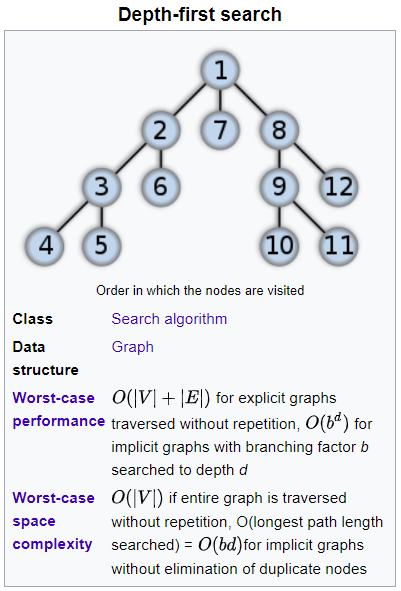
\includegraphics{source/lesson6_binarytree_DFS.png}
\item
  Breadth-First Search (BFS):
  \href{https://en.wikipedia.org/wiki/Breadth-first_search}{wiki\_BFS}
  the priority is visiting every node on the same level we're currently
  on before visiting child nodes. Breadth-first search (BFS) is an
  algorithm for traversing or searching tree or graph data structures.
  It starts at the tree root (or some arbitrary node of a graph,
  sometimes referred to as a 'search key'), and explores all of the
  neighbor nodes at the present depth prior to moving on to the nodes at
  the next depth level.
  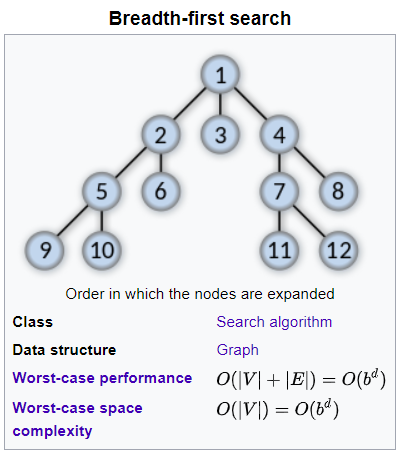
\includegraphics{source/lesson6_binarytree_BFS.png}
\end{itemize}

    \paragraph{Depth-First Search}\label{depth-first-search}

These searches are referred to as depth-first search (DFS), as the
search tree is deepened as much as possible on each child before going
to the next sibling. For a binary tree, they are defined as display
operations recursively at each node, starting with the root, whose
algorithm is as follows:

The general recursive pattern for traversing a (non-empty) binary tree
is this: At node N do the following: * (L) Recursively traverse its left
subtree. This step is finished at the node N again. * (R) Recursively
traverse its right subtree. This step is finished at the node N again. *
(N) Process N itself.

These steps can be done in any order. If (L) is done before (R), the
process is called left-to-right traversal, otherwise it is called
right-to-left traversal. The following methods show left-to-right
traversal: * Pre-Order Traversal: check off a node as you see it before
you traverse any further in the tree
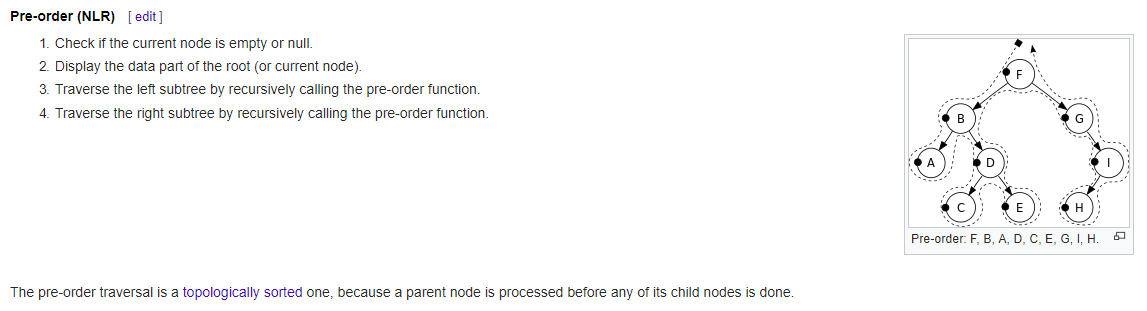
\includegraphics{source/lesson6_binarytree_DFS_preorder.png} * In-Order
Traversal: check off a node after you traverse its left child
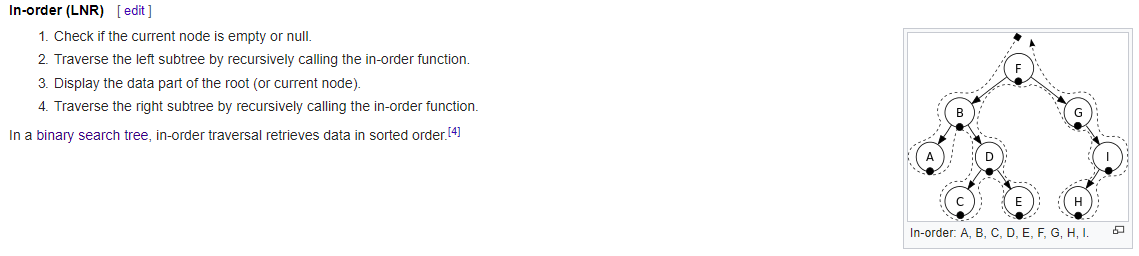
\includegraphics{source/lesson6_binarytree_DFS_inorder.png} * Post-Order
Traversal: check off a node only after you traverse all of its
descendants
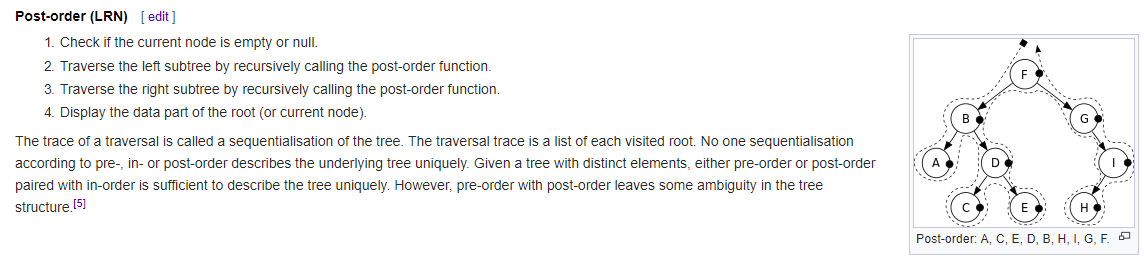
\includegraphics{source/lesson6_binarytree_DFS_postorder.png}

    \paragraph{Divide Conquer Algorithm}\label{divide-conquer-algorithm}

Traverse v.s. Divide Conquer (拆解结合) * They are both recursion
algorithm * Result in parameter v.s. Result in return value * Top down
v.s. Bottom Up

    \paragraph{Question 1.1: Pre-Order Traversal
(先序{[}根{]}遍历)}\label{question-1.1-pre-order-traversal-ux5148ux5e8fux6839ux904dux5386}

\emph{Solution 1}: Recursion

先处理自己,再左子节点,最后右子节点

\begin{verbatim}
                10 == root
               /  \
              5    15
             / \   / \
            2  7  12 20     <-- all leaf node's level == 3

10, 5, 2,7, 15, 12, 20
\end{verbatim}

\emph{Solution 2}: Iteration

\begin{verbatim}
                 A == root
               /   \
              B     C
             / \   / \ 
            N   N N   N     

第一次访问节点的时候打印
(A, 1) print --> (B, 1) print --> (A, 2) --> (C, 1) print
\end{verbatim}

    \begin{Verbatim}[commandchars=\\\{\}]
{\color{incolor}In [{\color{incolor}72}]:} \PY{k}{class} \PY{n+nc}{Traversal}\PY{p}{(}\PY{n+nb}{object}\PY{p}{)}\PY{p}{:}
             \PY{k}{def} \PY{n+nf}{preorder\PYZus{}traverse}\PY{p}{(}\PY{n+nb+bp}{self}\PY{p}{,} \PY{n}{root}\PY{p}{)}\PY{p}{:}
                 \PY{l+s+sd}{\PYZdq{}\PYZdq{}\PYZdq{}}
         \PY{l+s+sd}{        \PYZsh{} Time Complexity: O(n)}
         \PY{l+s+sd}{        \PYZsh{} Space Complexity: O(h)  h \PYZhy{} height of the binary tree}
         \PY{l+s+sd}{        \PYZdq{}\PYZdq{}\PYZdq{}}
                 \PY{k}{if} \PY{o+ow}{not} \PY{n}{root}\PY{p}{:}
                     \PY{k}{return} \PY{p}{[}\PY{p}{]}
                 
                 \PY{n}{res} \PY{o}{=} \PY{p}{[}\PY{p}{]}
                 \PY{n+nb+bp}{self}\PY{o}{.}\PY{n}{helper}\PY{p}{(}\PY{n}{root}\PY{p}{,} \PY{n}{res}\PY{p}{)}
                 \PY{k}{return} \PY{n}{res}
                 
             \PY{k}{def} \PY{n+nf}{helper}\PY{p}{(}\PY{n+nb+bp}{self}\PY{p}{,} \PY{n}{root}\PY{p}{,} \PY{n}{res}\PY{p}{)}\PY{p}{:}
                 \PY{c+c1}{\PYZsh{} Base Case}
                 \PY{k}{if} \PY{o+ow}{not} \PY{n}{root}\PY{p}{:}
                     \PY{k}{return}
                 
                 \PY{c+c1}{\PYZsh{} Recursion Part}
                 \PY{n}{res}\PY{o}{.}\PY{n}{append}\PY{p}{(}\PY{n}{root}\PY{o}{.}\PY{n}{val}\PY{p}{)}
                 \PY{n+nb+bp}{self}\PY{o}{.}\PY{n}{helper}\PY{p}{(}\PY{n}{root}\PY{o}{.}\PY{n}{left}\PY{p}{,} \PY{n}{res}\PY{p}{)}
                 \PY{n+nb+bp}{self}\PY{o}{.}\PY{n}{helper}\PY{p}{(}\PY{n}{root}\PY{o}{.}\PY{n}{right}\PY{p}{,} \PY{n}{res}\PY{p}{)}
                 
             \PY{k}{def} \PY{n+nf}{preorder\PYZus{}divideconquer}\PY{p}{(}\PY{n+nb+bp}{self}\PY{p}{,} \PY{n}{root}\PY{p}{)}\PY{p}{:}
                 \PY{l+s+sd}{\PYZdq{}\PYZdq{}\PYZdq{}}
         \PY{l+s+sd}{        \PYZsh{} Time Complexity: O(n)}
         \PY{l+s+sd}{        \PYZsh{} Space Complexity: O(h)  h \PYZhy{} height of the binary tree}
         \PY{l+s+sd}{        \PYZdq{}\PYZdq{}\PYZdq{}}
                 \PY{k}{if} \PY{o+ow}{not} \PY{n}{root}\PY{p}{:}
                     \PY{k}{return} \PY{p}{[}\PY{p}{]}
                 
                 \PY{c+c1}{\PYZsh{} what to get from yoour children \PYZhy{}\PYZhy{} divide}
                 \PY{n}{left\PYZus{}res} \PY{o}{=} \PY{n+nb+bp}{self}\PY{o}{.}\PY{n}{preorder\PYZus{}divideconquer}\PY{p}{(}\PY{n}{root}\PY{o}{.}\PY{n}{left}\PY{p}{)}
                 \PY{n}{right\PYZus{}res} \PY{o}{=} \PY{n+nb+bp}{self}\PY{o}{.}\PY{n}{preorder\PYZus{}divideconquer}\PY{p}{(}\PY{n}{root}\PY{o}{.}\PY{n}{right}\PY{p}{)}
                 
                 \PY{c+c1}{\PYZsh{} what to do in the current stage \PYZhy{}\PYZhy{} conquer}
                 \PY{n}{results} \PY{o}{=} \PY{p}{[}\PY{p}{]}
                 \PY{n}{results}\PY{o}{.}\PY{n}{append}\PY{p}{(}\PY{n}{root}\PY{o}{.}\PY{n}{val}\PY{p}{)}
                 \PY{k}{if} \PY{n}{left\PYZus{}res}\PY{p}{:}
                     \PY{n}{results}\PY{o}{.}\PY{n}{extend}\PY{p}{(}\PY{n}{left\PYZus{}res}\PY{p}{)}
                 \PY{k}{if} \PY{n}{right\PYZus{}res}\PY{p}{:}
                     \PY{n}{results}\PY{o}{.}\PY{n}{extend}\PY{p}{(}\PY{n}{right\PYZus{}res}\PY{p}{)}
                 
                 \PY{c+c1}{\PYZsh{} what to return to your parent}
                 \PY{k}{return} \PY{n}{results}
                 
             \PY{k}{def} \PY{n+nf}{preorder\PYZus{}iter}\PY{p}{(}\PY{n+nb+bp}{self}\PY{p}{,} \PY{n}{root}\PY{p}{)}\PY{p}{:}
                 \PY{k}{if} \PY{o+ow}{not} \PY{n}{root}\PY{p}{:}
                     \PY{k}{return} \PY{p}{[}\PY{p}{]}
                 
                 \PY{n}{results} \PY{o}{=} \PY{p}{[}\PY{p}{]}
                 \PY{n}{stack} \PY{o}{=} \PY{p}{[}\PY{p}{(}\PY{n}{root}\PY{p}{,} \PY{l+m+mi}{1}\PY{p}{)}\PY{p}{]}  \PY{c+c1}{\PYZsh{} the first time to visit root node, (node, count)}
                 \PY{k}{while} \PY{n}{stack}\PY{p}{:}
                     \PY{n}{node}\PY{p}{,} \PY{n}{count} \PY{o}{=} \PY{n}{stack}\PY{o}{.}\PY{n}{pop}\PY{p}{(}\PY{p}{)}
                     \PY{k}{if} \PY{n}{count} \PY{o}{==} \PY{l+m+mi}{1}\PY{p}{:}
                         \PY{n}{results}\PY{o}{.}\PY{n}{append}\PY{p}{(}\PY{n}{node}\PY{o}{.}\PY{n}{val}\PY{p}{)}
                         
                         \PY{c+c1}{\PYZsh{} for the visit of the second time (A, 2) \PYZhy{}\PYZhy{} \PYZgt{} (C, 1)}
                         \PY{n}{stack}\PY{o}{.}\PY{n}{append}\PY{p}{(}\PY{p}{(}\PY{n}{node}\PY{p}{,} \PY{n}{count} \PY{o}{+} \PY{l+m+mi}{1}\PY{p}{)}\PY{p}{)}
                         
                         \PY{c+c1}{\PYZsh{} add left node (B, 1)}
                         \PY{k}{if} \PY{n}{node}\PY{o}{.}\PY{n}{left}\PY{p}{:}
                             \PY{n}{stack}\PY{o}{.}\PY{n}{append}\PY{p}{(}\PY{p}{(}\PY{n}{node}\PY{o}{.}\PY{n}{left}\PY{p}{,} \PY{l+m+mi}{1}\PY{p}{)}\PY{p}{)}
                             
                     \PY{k}{elif} \PY{n}{count} \PY{o}{==} \PY{l+m+mi}{2}\PY{p}{:}
                         \PY{c+c1}{\PYZsh{} add right node (C, 1)}
                         \PY{k}{if} \PY{n}{node}\PY{o}{.}\PY{n}{right}\PY{p}{:}
                             \PY{n}{stack}\PY{o}{.}\PY{n}{append}\PY{p}{(}\PY{p}{(}\PY{n}{node}\PY{o}{.}\PY{n}{right}\PY{p}{,} \PY{l+m+mi}{1}\PY{p}{)}\PY{p}{)}
                             
                 \PY{k}{return} \PY{n}{results}
                 
         \PY{k}{if} \PY{n+nv+vm}{\PYZus{}\PYZus{}name\PYZus{}\PYZus{}} \PY{o}{==} \PY{l+s+s2}{\PYZdq{}}\PY{l+s+s2}{\PYZus{}\PYZus{}main\PYZus{}\PYZus{}}\PY{l+s+s2}{\PYZdq{}}\PY{p}{:}
             \PY{n}{root} \PY{o}{=} \PY{n}{TreeNode}\PY{p}{(}\PY{l+m+mi}{10}\PY{p}{)}
             \PY{n}{root}\PY{o}{.}\PY{n}{left} \PY{o}{=} \PY{n}{TreeNode}\PY{p}{(}\PY{l+m+mi}{5}\PY{p}{)}
             \PY{n}{root}\PY{o}{.}\PY{n}{right} \PY{o}{=} \PY{n}{TreeNode}\PY{p}{(}\PY{l+m+mi}{15}\PY{p}{)}
             \PY{n}{root}\PY{o}{.}\PY{n}{left}\PY{o}{.}\PY{n}{left} \PY{o}{=} \PY{n}{TreeNode}\PY{p}{(}\PY{l+m+mi}{2}\PY{p}{)}
             \PY{n}{root}\PY{o}{.}\PY{n}{left}\PY{o}{.}\PY{n}{right} \PY{o}{=} \PY{n}{TreeNode}\PY{p}{(}\PY{l+m+mi}{7}\PY{p}{)}
             \PY{n}{root}\PY{o}{.}\PY{n}{right}\PY{o}{.}\PY{n}{left} \PY{o}{=} \PY{n}{TreeNode}\PY{p}{(}\PY{l+m+mi}{12}\PY{p}{)}
             \PY{n}{root}\PY{o}{.}\PY{n}{right}\PY{o}{.}\PY{n}{right} \PY{o}{=} \PY{n}{TreeNode}\PY{p}{(}\PY{l+m+mi}{20}\PY{p}{)}
         
             \PY{n}{soln} \PY{o}{=} \PY{n}{Traversal}\PY{p}{(}\PY{p}{)}
             \PY{n+nb}{print}\PY{p}{(}\PY{n}{soln}\PY{o}{.}\PY{n}{preorder\PYZus{}traverse}\PY{p}{(}\PY{n}{root}\PY{p}{)}\PY{p}{)}
             \PY{n+nb}{print}\PY{p}{(}\PY{n}{soln}\PY{o}{.}\PY{n}{preorder\PYZus{}divideconquer}\PY{p}{(}\PY{n}{root}\PY{p}{)}\PY{p}{)}
             \PY{n+nb}{print}\PY{p}{(}\PY{n}{soln}\PY{o}{.}\PY{n}{preorder\PYZus{}iter}\PY{p}{(}\PY{n}{root}\PY{p}{)}\PY{p}{)}
\end{Verbatim}


    \begin{Verbatim}[commandchars=\\\{\}]
[10, 5, 2, 7, 15, 12, 20]
[10, 5, 2, 7, 15, 12, 20]
[10, 5, 2, 7, 15, 12, 20]

    \end{Verbatim}

    \paragraph{Question 1.2: In-Order Traversal
(中序{[}根{]}遍历)}\label{question-1.2-in-order-traversal-ux4e2dux5e8fux6839ux904dux5386}

\emph{Solution 1}: Recursion

先左子节点,再处理自己,最后右子节点

\begin{verbatim}
                10 == root
               /  \
              5    15
             / \   / \
            2  7  12 20     <-- all leaf node's level == 3

2, 5, 7, 10, 12, 15, 20
\end{verbatim}

\emph{Solution 2}: Iteration

\begin{verbatim}
                 A == root
               /   \
              B     C
             / \   / \ 
            N   N N   N     

第二次访问节点的时候打印
(A, 1) --> (B, 1) --> N --> (B, 2) print --> N -->
--> (A, 2) print --> (C, 1) --> N --> (C, 2) print --> N
\end{verbatim}

    \begin{Verbatim}[commandchars=\\\{\}]
{\color{incolor}In [{\color{incolor}73}]:} \PY{k}{class} \PY{n+nc}{Traversal}\PY{p}{(}\PY{n+nb}{object}\PY{p}{)}\PY{p}{:}
             \PY{k}{def} \PY{n+nf}{inorder\PYZus{}traverse}\PY{p}{(}\PY{n+nb+bp}{self}\PY{p}{,} \PY{n}{root}\PY{p}{)}\PY{p}{:}
                 \PY{l+s+sd}{\PYZdq{}\PYZdq{}\PYZdq{}}
         \PY{l+s+sd}{        \PYZsh{} Time Complexity: O(n)}
         \PY{l+s+sd}{        \PYZsh{} Space Complexity: O(h)  h \PYZhy{} height of the binary tree}
         \PY{l+s+sd}{        \PYZdq{}\PYZdq{}\PYZdq{}}
                 \PY{k}{if} \PY{o+ow}{not} \PY{n}{root}\PY{p}{:}
                     \PY{k}{return} \PY{p}{[}\PY{p}{]}
                 
                 \PY{n}{res} \PY{o}{=} \PY{p}{[}\PY{p}{]}
                 \PY{n+nb+bp}{self}\PY{o}{.}\PY{n}{helper}\PY{p}{(}\PY{n}{root}\PY{p}{,} \PY{n}{res}\PY{p}{)}
                 \PY{k}{return} \PY{n}{res}
                 
             \PY{k}{def} \PY{n+nf}{helper}\PY{p}{(}\PY{n+nb+bp}{self}\PY{p}{,} \PY{n}{root}\PY{p}{,} \PY{n}{res}\PY{p}{)}\PY{p}{:}
                 \PY{c+c1}{\PYZsh{} Base Case}
                 \PY{k}{if} \PY{o+ow}{not} \PY{n}{root}\PY{p}{:}
                     \PY{k}{return}
                 
                 \PY{c+c1}{\PYZsh{} Recursion Part        }
                 \PY{n+nb+bp}{self}\PY{o}{.}\PY{n}{helper}\PY{p}{(}\PY{n}{root}\PY{o}{.}\PY{n}{left}\PY{p}{,} \PY{n}{res}\PY{p}{)}
                 \PY{n}{res}\PY{o}{.}\PY{n}{append}\PY{p}{(}\PY{n}{root}\PY{o}{.}\PY{n}{val}\PY{p}{)}
                 \PY{n+nb+bp}{self}\PY{o}{.}\PY{n}{helper}\PY{p}{(}\PY{n}{root}\PY{o}{.}\PY{n}{right}\PY{p}{,} \PY{n}{res}\PY{p}{)}
                 
             \PY{k}{def} \PY{n+nf}{inorder\PYZus{}divideconquer}\PY{p}{(}\PY{n+nb+bp}{self}\PY{p}{,} \PY{n}{root}\PY{p}{)}\PY{p}{:}
                 \PY{c+c1}{\PYZsh{} base case}
                 \PY{k}{if} \PY{o+ow}{not} \PY{n}{root}\PY{p}{:}
                     \PY{k}{return} \PY{p}{[}\PY{p}{]}
                 
                 \PY{c+c1}{\PYZsh{} what to get from your children \PYZhy{}\PYZhy{} divide}
                 \PY{n}{left\PYZus{}res} \PY{o}{=} \PY{n+nb+bp}{self}\PY{o}{.}\PY{n}{inorder\PYZus{}divideconquer}\PY{p}{(}\PY{n}{root}\PY{o}{.}\PY{n}{left}\PY{p}{)}
                 \PY{n}{right\PYZus{}res} \PY{o}{=} \PY{n+nb+bp}{self}\PY{o}{.}\PY{n}{inorder\PYZus{}divideconquer}\PY{p}{(}\PY{n}{root}\PY{o}{.}\PY{n}{right}\PY{p}{)}
                 
                 \PY{c+c1}{\PYZsh{} what to do in the current stage \PYZhy{}\PYZhy{} conquer}
                 \PY{n}{results} \PY{o}{=} \PY{p}{[}\PY{p}{]}
                 \PY{k}{if} \PY{n}{left\PYZus{}res}\PY{p}{:}
                     \PY{n}{results}\PY{o}{.}\PY{n}{extend}\PY{p}{(}\PY{n}{left\PYZus{}res}\PY{p}{)}
                 \PY{n}{results}\PY{o}{.}\PY{n}{append}\PY{p}{(}\PY{n}{root}\PY{o}{.}\PY{n}{val}\PY{p}{)}
                 \PY{k}{if} \PY{n}{right\PYZus{}res}\PY{p}{:}
                     \PY{n}{results}\PY{o}{.}\PY{n}{extend}\PY{p}{(}\PY{n}{right\PYZus{}res}\PY{p}{)}
                 
                 \PY{c+c1}{\PYZsh{} what to return to your parent}
                 \PY{k}{return} \PY{n}{results}
                 
             \PY{k}{def} \PY{n+nf}{inorder\PYZus{}iter}\PY{p}{(}\PY{n+nb+bp}{self}\PY{p}{,} \PY{n}{root}\PY{p}{)}\PY{p}{:}
                 \PY{k}{if} \PY{o+ow}{not} \PY{n}{root}\PY{p}{:}
                     \PY{k}{return} \PY{p}{[}\PY{p}{]}
                 
                 \PY{n}{results} \PY{o}{=} \PY{p}{[}\PY{p}{]}
                 \PY{n}{stack} \PY{o}{=} \PY{p}{[}\PY{p}{(}\PY{n}{root}\PY{p}{,} \PY{l+m+mi}{1}\PY{p}{)}\PY{p}{]}  \PY{c+c1}{\PYZsh{} the first time to visit root node, (node, count)}
                 \PY{k}{while} \PY{n}{stack}\PY{p}{:}
                     \PY{n}{node}\PY{p}{,} \PY{n}{count} \PY{o}{=} \PY{n}{stack}\PY{o}{.}\PY{n}{pop}\PY{p}{(}\PY{p}{)}
                     \PY{k}{if} \PY{n}{count} \PY{o}{==} \PY{l+m+mi}{1}\PY{p}{:}
                         \PY{c+c1}{\PYZsh{} for the visit of the second time (A, 2) \PYZhy{}\PYZhy{} \PYZgt{} (C, 1)}
                         \PY{n}{stack}\PY{o}{.}\PY{n}{append}\PY{p}{(}\PY{p}{(}\PY{n}{node}\PY{p}{,} \PY{n}{count} \PY{o}{+} \PY{l+m+mi}{1}\PY{p}{)}\PY{p}{)}
                         
                         \PY{c+c1}{\PYZsh{} add left node (B, 1)}
                         \PY{k}{if} \PY{n}{node}\PY{o}{.}\PY{n}{left}\PY{p}{:}
                             \PY{n}{stack}\PY{o}{.}\PY{n}{append}\PY{p}{(}\PY{p}{(}\PY{n}{node}\PY{o}{.}\PY{n}{left}\PY{p}{,} \PY{l+m+mi}{1}\PY{p}{)}\PY{p}{)}
                             
                     \PY{k}{elif} \PY{n}{count} \PY{o}{==} \PY{l+m+mi}{2}\PY{p}{:}
                         \PY{n}{results}\PY{o}{.}\PY{n}{append}\PY{p}{(}\PY{n}{node}\PY{o}{.}\PY{n}{val}\PY{p}{)}
                         \PY{c+c1}{\PYZsh{} add right node (C, 1)}
                         \PY{k}{if} \PY{n}{node}\PY{o}{.}\PY{n}{right}\PY{p}{:}
                             \PY{n}{stack}\PY{o}{.}\PY{n}{append}\PY{p}{(}\PY{p}{(}\PY{n}{node}\PY{o}{.}\PY{n}{right}\PY{p}{,} \PY{l+m+mi}{1}\PY{p}{)}\PY{p}{)}
                             
                 \PY{k}{return} \PY{n}{results}
                 
         \PY{k}{if} \PY{n+nv+vm}{\PYZus{}\PYZus{}name\PYZus{}\PYZus{}} \PY{o}{==} \PY{l+s+s2}{\PYZdq{}}\PY{l+s+s2}{\PYZus{}\PYZus{}main\PYZus{}\PYZus{}}\PY{l+s+s2}{\PYZdq{}}\PY{p}{:}
             \PY{n}{root} \PY{o}{=} \PY{n}{TreeNode}\PY{p}{(}\PY{l+m+mi}{10}\PY{p}{)}
             \PY{n}{root}\PY{o}{.}\PY{n}{left} \PY{o}{=} \PY{n}{TreeNode}\PY{p}{(}\PY{l+m+mi}{5}\PY{p}{)}
             \PY{n}{root}\PY{o}{.}\PY{n}{right} \PY{o}{=} \PY{n}{TreeNode}\PY{p}{(}\PY{l+m+mi}{15}\PY{p}{)}
             \PY{n}{root}\PY{o}{.}\PY{n}{left}\PY{o}{.}\PY{n}{left} \PY{o}{=} \PY{n}{TreeNode}\PY{p}{(}\PY{l+m+mi}{2}\PY{p}{)}
             \PY{n}{root}\PY{o}{.}\PY{n}{left}\PY{o}{.}\PY{n}{right} \PY{o}{=} \PY{n}{TreeNode}\PY{p}{(}\PY{l+m+mi}{7}\PY{p}{)}
             \PY{n}{root}\PY{o}{.}\PY{n}{right}\PY{o}{.}\PY{n}{left} \PY{o}{=} \PY{n}{TreeNode}\PY{p}{(}\PY{l+m+mi}{12}\PY{p}{)}
             \PY{n}{root}\PY{o}{.}\PY{n}{right}\PY{o}{.}\PY{n}{right} \PY{o}{=} \PY{n}{TreeNode}\PY{p}{(}\PY{l+m+mi}{20}\PY{p}{)}
         
             \PY{n}{soln} \PY{o}{=} \PY{n}{Traversal}\PY{p}{(}\PY{p}{)}
             \PY{n+nb}{print}\PY{p}{(}\PY{n}{soln}\PY{o}{.}\PY{n}{inorder\PYZus{}traverse}\PY{p}{(}\PY{n}{root}\PY{p}{)}\PY{p}{)}
             \PY{n+nb}{print}\PY{p}{(}\PY{n}{soln}\PY{o}{.}\PY{n}{inorder\PYZus{}divideconquer}\PY{p}{(}\PY{n}{root}\PY{p}{)}\PY{p}{)}
             \PY{n+nb}{print}\PY{p}{(}\PY{n}{soln}\PY{o}{.}\PY{n}{inorder\PYZus{}iter}\PY{p}{(}\PY{n}{root}\PY{p}{)}\PY{p}{)}
\end{Verbatim}


    \begin{Verbatim}[commandchars=\\\{\}]
[2, 5, 7, 10, 12, 15, 20]
[2, 5, 7, 10, 12, 15, 20]
[2, 5, 7, 10, 12, 15, 20]

    \end{Verbatim}

    \paragraph{Question 1.3: Post-Order Traversal
(后序{[}根{]}遍历)}\label{question-1.3-post-order-traversal-ux540eux5e8fux6839ux904dux5386}

\emph{Solution 1}: Recursion

先左子节点,再右子节点,最后处理自己

\begin{verbatim}
                10 == root
               /  \
              5    15
             / \   / \
            2  7  12 20     <-- all leaf node's level == 3

2, 7, 5, 12, 20, 15, 10
\end{verbatim}

\emph{Solution 2}: Iteration

\begin{verbatim}
                 A == root
               /   \
              B     C
             / \   / \ 
            N   N N   N     

第三次访问节点的时候打印
(A, 1) --> (B, 1) --> N --> (B, 2) --> N --> (B, 3) print -->
--> (A, 2) --> (C, 1) --> N --> (C, 2)  --> N --> (C, 3) print --> 
--> (A, 3) print
\end{verbatim}

    \begin{Verbatim}[commandchars=\\\{\}]
{\color{incolor}In [{\color{incolor}74}]:} \PY{k}{class} \PY{n+nc}{Traversal}\PY{p}{(}\PY{n+nb}{object}\PY{p}{)}\PY{p}{:}
             \PY{k}{def} \PY{n+nf}{postorder\PYZus{}traverse}\PY{p}{(}\PY{n+nb+bp}{self}\PY{p}{,} \PY{n}{root}\PY{p}{)}\PY{p}{:}
                 \PY{l+s+sd}{\PYZdq{}\PYZdq{}\PYZdq{}}
         \PY{l+s+sd}{        \PYZsh{} Time Complexity: O(n)}
         \PY{l+s+sd}{        \PYZsh{} Space Complexity: O(h)  h \PYZhy{} height of the binary tree}
         \PY{l+s+sd}{        \PYZdq{}\PYZdq{}\PYZdq{}}
                 \PY{k}{if} \PY{o+ow}{not} \PY{n}{root}\PY{p}{:}
                     \PY{k}{return} \PY{p}{[}\PY{p}{]}
                 
                 \PY{n}{res} \PY{o}{=} \PY{p}{[}\PY{p}{]}
                 \PY{n+nb+bp}{self}\PY{o}{.}\PY{n}{helper}\PY{p}{(}\PY{n}{root}\PY{p}{,} \PY{n}{res}\PY{p}{)}
                 \PY{k}{return} \PY{n}{res}
                 
             \PY{k}{def} \PY{n+nf}{helper}\PY{p}{(}\PY{n+nb+bp}{self}\PY{p}{,} \PY{n}{root}\PY{p}{,} \PY{n}{res}\PY{p}{)}\PY{p}{:}
                 \PY{c+c1}{\PYZsh{} Base Case}
                 \PY{k}{if} \PY{o+ow}{not} \PY{n}{root}\PY{p}{:}
                     \PY{k}{return}
                 
                 \PY{c+c1}{\PYZsh{} Recursion Part        }
                 \PY{n+nb+bp}{self}\PY{o}{.}\PY{n}{helper}\PY{p}{(}\PY{n}{root}\PY{o}{.}\PY{n}{left}\PY{p}{,} \PY{n}{res}\PY{p}{)}
                 \PY{n+nb+bp}{self}\PY{o}{.}\PY{n}{helper}\PY{p}{(}\PY{n}{root}\PY{o}{.}\PY{n}{right}\PY{p}{,} \PY{n}{res}\PY{p}{)}
                 \PY{n}{res}\PY{o}{.}\PY{n}{append}\PY{p}{(}\PY{n}{root}\PY{o}{.}\PY{n}{val}\PY{p}{)}
                 
             \PY{k}{def} \PY{n+nf}{postorder\PYZus{}divideconquer}\PY{p}{(}\PY{n+nb+bp}{self}\PY{p}{,} \PY{n}{root}\PY{p}{)}\PY{p}{:}
                 \PY{c+c1}{\PYZsh{} base case}
                 \PY{k}{if} \PY{o+ow}{not} \PY{n}{root}\PY{p}{:}
                     \PY{k}{return} \PY{p}{[}\PY{p}{]}
                 
                 \PY{c+c1}{\PYZsh{} what to get from your children \PYZhy{}\PYZhy{} divide}
                 \PY{n}{left\PYZus{}res} \PY{o}{=} \PY{n+nb+bp}{self}\PY{o}{.}\PY{n}{postorder\PYZus{}divideconquer}\PY{p}{(}\PY{n}{root}\PY{o}{.}\PY{n}{left}\PY{p}{)}
                 \PY{n}{right\PYZus{}res} \PY{o}{=} \PY{n+nb+bp}{self}\PY{o}{.}\PY{n}{postorder\PYZus{}divideconquer}\PY{p}{(}\PY{n}{root}\PY{o}{.}\PY{n}{right}\PY{p}{)}
                 
                 \PY{c+c1}{\PYZsh{} what to do in the current stage \PYZhy{}\PYZhy{} conquer}
                 \PY{n}{results} \PY{o}{=} \PY{p}{[}\PY{p}{]}
                 \PY{k}{if} \PY{n}{left\PYZus{}res}\PY{p}{:}
                     \PY{n}{results}\PY{o}{.}\PY{n}{extend}\PY{p}{(}\PY{n}{left\PYZus{}res}\PY{p}{)}        
                 \PY{k}{if} \PY{n}{right\PYZus{}res}\PY{p}{:}
                     \PY{n}{results}\PY{o}{.}\PY{n}{extend}\PY{p}{(}\PY{n}{right\PYZus{}res}\PY{p}{)}
                 \PY{n}{results}\PY{o}{.}\PY{n}{append}\PY{p}{(}\PY{n}{root}\PY{o}{.}\PY{n}{val}\PY{p}{)}
                 
                 \PY{c+c1}{\PYZsh{} what to return to your parent}
                 \PY{k}{return} \PY{n}{results}
             
             \PY{k}{def} \PY{n+nf}{postorder\PYZus{}iter}\PY{p}{(}\PY{n+nb+bp}{self}\PY{p}{,} \PY{n}{root}\PY{p}{)}\PY{p}{:}
                 \PY{k}{if} \PY{o+ow}{not} \PY{n}{root}\PY{p}{:}
                     \PY{k}{return} \PY{p}{[}\PY{p}{]}
                 
                 \PY{n}{results} \PY{o}{=} \PY{p}{[}\PY{p}{]}
                 \PY{n}{stack} \PY{o}{=} \PY{p}{[}\PY{p}{(}\PY{n}{root}\PY{p}{,} \PY{l+m+mi}{1}\PY{p}{)}\PY{p}{]}  \PY{c+c1}{\PYZsh{} the first time to visit root node, (node, count)}
                 \PY{k}{while} \PY{n}{stack}\PY{p}{:}
                     \PY{n}{node}\PY{p}{,} \PY{n}{count} \PY{o}{=} \PY{n}{stack}\PY{o}{.}\PY{n}{pop}\PY{p}{(}\PY{p}{)}
                     \PY{k}{if} \PY{n}{count} \PY{o}{==} \PY{l+m+mi}{1}\PY{p}{:}
                         \PY{c+c1}{\PYZsh{} for the visit of the second time (A, 2) \PYZhy{}\PYZhy{} \PYZgt{} (C, 1)}
                         \PY{n}{stack}\PY{o}{.}\PY{n}{append}\PY{p}{(}\PY{p}{(}\PY{n}{node}\PY{p}{,} \PY{n}{count} \PY{o}{+} \PY{l+m+mi}{1}\PY{p}{)}\PY{p}{)}
                         
                         \PY{c+c1}{\PYZsh{} add left node (B, 1)}
                         \PY{k}{if} \PY{n}{node}\PY{o}{.}\PY{n}{left}\PY{p}{:}
                             \PY{n}{stack}\PY{o}{.}\PY{n}{append}\PY{p}{(}\PY{p}{(}\PY{n}{node}\PY{o}{.}\PY{n}{left}\PY{p}{,} \PY{l+m+mi}{1}\PY{p}{)}\PY{p}{)}
                             
                     \PY{k}{elif} \PY{n}{count} \PY{o}{==} \PY{l+m+mi}{2}\PY{p}{:}
                         \PY{c+c1}{\PYZsh{} for the visit of the third time (A, 3) \PYZhy{}\PYZhy{} \PYZgt{} print}
                         \PY{n}{stack}\PY{o}{.}\PY{n}{append}\PY{p}{(}\PY{p}{(}\PY{n}{node}\PY{p}{,} \PY{n}{count} \PY{o}{+} \PY{l+m+mi}{1}\PY{p}{)}\PY{p}{)}
                         
                         \PY{c+c1}{\PYZsh{} add right node (C, 1)}
                         \PY{k}{if} \PY{n}{node}\PY{o}{.}\PY{n}{right}\PY{p}{:}
                             \PY{n}{stack}\PY{o}{.}\PY{n}{append}\PY{p}{(}\PY{p}{(}\PY{n}{node}\PY{o}{.}\PY{n}{right}\PY{p}{,} \PY{l+m+mi}{1}\PY{p}{)}\PY{p}{)}
                             
                     \PY{k}{elif} \PY{n}{count} \PY{o}{==} \PY{l+m+mi}{3}\PY{p}{:}
                         \PY{n}{results}\PY{o}{.}\PY{n}{append}\PY{p}{(}\PY{n}{node}\PY{o}{.}\PY{n}{val}\PY{p}{)}
                             
                 \PY{k}{return} \PY{n}{results}
                 
         \PY{k}{if} \PY{n+nv+vm}{\PYZus{}\PYZus{}name\PYZus{}\PYZus{}} \PY{o}{==} \PY{l+s+s2}{\PYZdq{}}\PY{l+s+s2}{\PYZus{}\PYZus{}main\PYZus{}\PYZus{}}\PY{l+s+s2}{\PYZdq{}}\PY{p}{:}
             \PY{n}{root} \PY{o}{=} \PY{n}{TreeNode}\PY{p}{(}\PY{l+m+mi}{10}\PY{p}{)}
             \PY{n}{root}\PY{o}{.}\PY{n}{left} \PY{o}{=} \PY{n}{TreeNode}\PY{p}{(}\PY{l+m+mi}{5}\PY{p}{)}
             \PY{n}{root}\PY{o}{.}\PY{n}{right} \PY{o}{=} \PY{n}{TreeNode}\PY{p}{(}\PY{l+m+mi}{15}\PY{p}{)}
             \PY{n}{root}\PY{o}{.}\PY{n}{left}\PY{o}{.}\PY{n}{left} \PY{o}{=} \PY{n}{TreeNode}\PY{p}{(}\PY{l+m+mi}{2}\PY{p}{)}
             \PY{n}{root}\PY{o}{.}\PY{n}{left}\PY{o}{.}\PY{n}{right} \PY{o}{=} \PY{n}{TreeNode}\PY{p}{(}\PY{l+m+mi}{7}\PY{p}{)}
             \PY{n}{root}\PY{o}{.}\PY{n}{right}\PY{o}{.}\PY{n}{left} \PY{o}{=} \PY{n}{TreeNode}\PY{p}{(}\PY{l+m+mi}{12}\PY{p}{)}
             \PY{n}{root}\PY{o}{.}\PY{n}{right}\PY{o}{.}\PY{n}{right} \PY{o}{=} \PY{n}{TreeNode}\PY{p}{(}\PY{l+m+mi}{20}\PY{p}{)}
         
             \PY{n}{soln} \PY{o}{=} \PY{n}{Traversal}\PY{p}{(}\PY{p}{)}
             \PY{n+nb}{print}\PY{p}{(}\PY{n}{soln}\PY{o}{.}\PY{n}{postorder\PYZus{}traverse}\PY{p}{(}\PY{n}{root}\PY{p}{)}\PY{p}{)}
             \PY{n+nb}{print}\PY{p}{(}\PY{n}{soln}\PY{o}{.}\PY{n}{postorder\PYZus{}divideconquer}\PY{p}{(}\PY{n}{root}\PY{p}{)}\PY{p}{)}
             \PY{n+nb}{print}\PY{p}{(}\PY{n}{soln}\PY{o}{.}\PY{n}{postorder\PYZus{}iter}\PY{p}{(}\PY{n}{root}\PY{p}{)}\PY{p}{)}
\end{Verbatim}


    \begin{Verbatim}[commandchars=\\\{\}]
[2, 7, 5, 12, 20, 15, 10]
[2, 7, 5, 12, 20, 15, 10]
[2, 7, 5, 12, 20, 15, 10]

    \end{Verbatim}

    \paragraph{Question 1.4: Level Order Traversal
(BFS)}\label{question-1.4-level-order-traversal-bfs}

\begin{verbatim}
10
5, 15
2, 7, 12, 20
1
\end{verbatim}

    \begin{Verbatim}[commandchars=\\\{\}]
{\color{incolor}In [{\color{incolor}77}]:} \PY{k}{class} \PY{n+nc}{Traversal}\PY{p}{(}\PY{n+nb}{object}\PY{p}{)}\PY{p}{:}
             \PY{k}{def} \PY{n+nf}{levelorder}\PY{p}{(}\PY{n+nb+bp}{self}\PY{p}{,} \PY{n}{root}\PY{p}{)}\PY{p}{:}
                 \PY{l+s+sd}{\PYZdq{}\PYZdq{}\PYZdq{}}
         \PY{l+s+sd}{        \PYZsh{} Time Complexity: O(n)}
         \PY{l+s+sd}{        \PYZsh{} Space Complexity: O(len(curr\PYZus{}level)+len(post\PYZus{}level)), O(n) at worst}
         \PY{l+s+sd}{        \PYZdq{}\PYZdq{}\PYZdq{}}
                 \PY{k}{if} \PY{o+ow}{not} \PY{n}{root}\PY{p}{:}
                     \PY{k}{return} \PY{p}{[}\PY{p}{]}
                 
                 \PY{n}{results} \PY{o}{=} \PY{p}{[}\PY{p}{]}        
                 
                 \PY{n}{frontier} \PY{o}{=} \PY{p}{[}\PY{n}{root}\PY{p}{]}
                 
                 \PY{k}{while} \PY{n}{frontier}\PY{p}{:}
                     \PY{n}{post} \PY{o}{=} \PY{p}{[}\PY{p}{]}
                     \PY{n}{solution} \PY{o}{=} \PY{p}{[}\PY{p}{]} \PY{c+c1}{\PYZsh{} for a certain level}
                     \PY{k}{for} \PY{n}{node} \PY{o+ow}{in} \PY{n}{frontier}\PY{p}{:}
                         \PY{n}{solution}\PY{o}{.}\PY{n}{append}\PY{p}{(}\PY{n}{node}\PY{o}{.}\PY{n}{val}\PY{p}{)}
                         \PY{k}{if} \PY{n}{node}\PY{o}{.}\PY{n}{left}\PY{p}{:}
                             \PY{n}{post}\PY{o}{.}\PY{n}{append}\PY{p}{(}\PY{n}{node}\PY{o}{.}\PY{n}{left}\PY{p}{)}
                         \PY{k}{if} \PY{n}{node}\PY{o}{.}\PY{n}{right}\PY{p}{:}
                             \PY{n}{post}\PY{o}{.}\PY{n}{append}\PY{p}{(}\PY{n}{node}\PY{o}{.}\PY{n}{right}\PY{p}{)}
                             
                     \PY{n}{frontier} \PY{o}{=} \PY{n}{post}
                     \PY{n}{results}\PY{o}{.}\PY{n}{append}\PY{p}{(}\PY{n}{solution}\PY{p}{)}
                     
                 \PY{k}{return} \PY{n}{results}
             
             \PY{k}{def} \PY{n+nf}{BFS\PYZus{}traversal}\PY{p}{(}\PY{n+nb+bp}{self}\PY{p}{,} \PY{n}{root}\PY{p}{)}\PY{p}{:}
                 \PY{c+c1}{\PYZsh{} Time Complexity: O(n)}
                 \PY{c+c1}{\PYZsh{} Space Complexity: O(len(curr\PYZus{}level)+len(post\PYZus{}level)), O(n) at worst}
                 \PY{k}{if} \PY{o+ow}{not} \PY{n}{root}\PY{p}{:}  \PY{c+c1}{\PYZsh{} if root is None}
                     \PY{k}{return} \PY{p}{[}\PY{p}{]}
                 
                 \PY{n}{results} \PY{o}{=} \PY{p}{[}\PY{p}{]} \PY{c+c1}{\PYZsh{} store the total results}
                 \PY{n}{result\PYZus{}level} \PY{o}{=} \PY{p}{[}\PY{p}{]} \PY{c+c1}{\PYZsh{} store the result of the current level}
                 
                 \PY{n}{curr\PYZus{}level} \PY{o}{=} \PY{p}{[}\PY{n}{root}\PY{p}{]}
                 \PY{n}{post\PYZus{}level} \PY{o}{=} \PY{p}{[}\PY{p}{]}
                 
                 \PY{k}{while} \PY{n}{curr\PYZus{}level}\PY{p}{:}  \PY{c+c1}{\PYZsh{} if curr\PYZus{}level is not None}
                     \PY{n}{head} \PY{o}{=} \PY{n}{curr\PYZus{}level}\PY{o}{.}\PY{n}{pop}\PY{p}{(}\PY{l+m+mi}{0}\PY{p}{)}
                     \PY{k}{if} \PY{o+ow}{not} \PY{n}{head}\PY{p}{:}
                         \PY{n}{result\PYZus{}level}\PY{o}{.}\PY{n}{append}\PY{p}{(}\PY{l+s+s2}{\PYZdq{}}\PY{l+s+s2}{\PYZsh{}}\PY{l+s+s2}{\PYZdq{}}\PY{p}{)}
                     \PY{k}{else}\PY{p}{:}                
                         \PY{n}{result\PYZus{}level}\PY{o}{.}\PY{n}{append}\PY{p}{(}\PY{n}{head}\PY{o}{.}\PY{n}{val}\PY{p}{)}
                         
                         \PY{k}{if} \PY{n}{head}\PY{o}{.}\PY{n}{left}\PY{p}{:} \PY{c+c1}{\PYZsh{} if head.left is not None}
                             \PY{n}{post\PYZus{}level}\PY{o}{.}\PY{n}{append}\PY{p}{(}\PY{n}{head}\PY{o}{.}\PY{n}{left}\PY{p}{)}
                         \PY{k}{else}\PY{p}{:}
                             \PY{n}{post\PYZus{}level}\PY{o}{.}\PY{n}{append}\PY{p}{(}\PY{k+kc}{None}\PY{p}{)}
                         
                         \PY{k}{if} \PY{n}{head}\PY{o}{.}\PY{n}{right}\PY{p}{:} \PY{c+c1}{\PYZsh{} if head.right is not None:}
                             \PY{n}{post\PYZus{}level}\PY{o}{.}\PY{n}{append}\PY{p}{(}\PY{n}{head}\PY{o}{.}\PY{n}{right}\PY{p}{)}
                         \PY{k}{else}\PY{p}{:}
                             \PY{n}{post\PYZus{}level}\PY{o}{.}\PY{n}{append}\PY{p}{(}\PY{k+kc}{None}\PY{p}{)}            
                     
                     \PY{k}{if} \PY{o+ow}{not} \PY{n}{curr\PYZus{}level}\PY{p}{:}  \PY{c+c1}{\PYZsh{} if curr\PYZus{}level is None}
                         \PY{n}{results}\PY{o}{.}\PY{n}{append}\PY{p}{(}\PY{n}{result\PYZus{}level}\PY{p}{)}
                         \PY{k}{if} \PY{n}{post\PYZus{}level} \PY{o+ow}{and} \PY{n+nb+bp}{self}\PY{o}{.}\PY{n}{not\PYZus{}all\PYZus{}none\PYZus{}check}\PY{p}{(}\PY{n}{post\PYZus{}level}\PY{p}{)} \PY{p}{:}  \PY{c+c1}{\PYZsh{} if post\PYZus{}level is not None}
                             \PY{n}{curr\PYZus{}level} \PY{o}{=} \PY{n}{post\PYZus{}level}
                             \PY{n}{post\PYZus{}level} \PY{o}{=} \PY{p}{[}\PY{p}{]}
                             \PY{n}{result\PYZus{}level} \PY{o}{=} \PY{p}{[}\PY{p}{]}
                             
                 \PY{k}{return} \PY{n}{results}
             
             \PY{k}{def} \PY{n+nf}{not\PYZus{}all\PYZus{}none\PYZus{}check}\PY{p}{(}\PY{n+nb+bp}{self}\PY{p}{,} \PY{n}{lst}\PY{p}{)}\PY{p}{:}
                 \PY{k}{if} \PY{o+ow}{not} \PY{n}{lst}\PY{p}{:}
                     \PY{k}{return} \PY{k+kc}{False}
                 
                 \PY{k}{for} \PY{n}{val} \PY{o+ow}{in} \PY{n}{lst}\PY{p}{:}
                     \PY{k}{if} \PY{n}{val} \PY{o+ow}{is} \PY{o+ow}{not} \PY{k+kc}{None}\PY{p}{:}
                         \PY{k}{return} \PY{k+kc}{True}
                     
                 \PY{k}{return} \PY{k+kc}{False}
             
         \PY{k}{if} \PY{n+nv+vm}{\PYZus{}\PYZus{}name\PYZus{}\PYZus{}} \PY{o}{==} \PY{l+s+s2}{\PYZdq{}}\PY{l+s+s2}{\PYZus{}\PYZus{}main\PYZus{}\PYZus{}}\PY{l+s+s2}{\PYZdq{}}\PY{p}{:}
             \PY{n}{root} \PY{o}{=} \PY{n}{TreeNode}\PY{p}{(}\PY{l+m+mi}{10}\PY{p}{)}
             \PY{n}{root}\PY{o}{.}\PY{n}{left} \PY{o}{=} \PY{n}{TreeNode}\PY{p}{(}\PY{l+m+mi}{5}\PY{p}{)}
             \PY{n}{root}\PY{o}{.}\PY{n}{right} \PY{o}{=} \PY{n}{TreeNode}\PY{p}{(}\PY{l+m+mi}{15}\PY{p}{)}
             \PY{n}{root}\PY{o}{.}\PY{n}{left}\PY{o}{.}\PY{n}{left} \PY{o}{=} \PY{n}{TreeNode}\PY{p}{(}\PY{l+m+mi}{2}\PY{p}{)}
             \PY{n}{root}\PY{o}{.}\PY{n}{left}\PY{o}{.}\PY{n}{right} \PY{o}{=} \PY{n}{TreeNode}\PY{p}{(}\PY{l+m+mi}{7}\PY{p}{)}
             \PY{n}{root}\PY{o}{.}\PY{n}{right}\PY{o}{.}\PY{n}{left} \PY{o}{=} \PY{n}{TreeNode}\PY{p}{(}\PY{l+m+mi}{12}\PY{p}{)}
             \PY{n}{root}\PY{o}{.}\PY{n}{right}\PY{o}{.}\PY{n}{right} \PY{o}{=} \PY{n}{TreeNode}\PY{p}{(}\PY{l+m+mi}{20}\PY{p}{)}
         
             \PY{n}{soln} \PY{o}{=} \PY{n}{Traversal}\PY{p}{(}\PY{p}{)}
             \PY{n+nb}{print}\PY{p}{(}\PY{n}{soln}\PY{o}{.}\PY{n}{levelorder}\PY{p}{(}\PY{n}{root}\PY{p}{)}\PY{p}{)}
             \PY{n+nb}{print}\PY{p}{(}\PY{n}{soln}\PY{o}{.}\PY{n}{BFS\PYZus{}traversal}\PY{p}{(}\PY{n}{root}\PY{p}{)}\PY{p}{)}
             
             \PY{n}{root} \PY{o}{=} \PY{n}{TreeNode}\PY{p}{(}\PY{l+m+mi}{10}\PY{p}{)}
             \PY{n}{root}\PY{o}{.}\PY{n}{left} \PY{o}{=} \PY{n}{TreeNode}\PY{p}{(}\PY{l+m+mi}{5}\PY{p}{)}
             \PY{n}{root}\PY{o}{.}\PY{n}{right} \PY{o}{=} \PY{n}{TreeNode}\PY{p}{(}\PY{l+m+mi}{15}\PY{p}{)}
             \PY{c+c1}{\PYZsh{}root.left.left = TreeNode(2)}
             \PY{n}{root}\PY{o}{.}\PY{n}{left}\PY{o}{.}\PY{n}{right} \PY{o}{=} \PY{n}{TreeNode}\PY{p}{(}\PY{l+m+mi}{7}\PY{p}{)}
             \PY{n}{root}\PY{o}{.}\PY{n}{right}\PY{o}{.}\PY{n}{left} \PY{o}{=} \PY{n}{TreeNode}\PY{p}{(}\PY{l+m+mi}{12}\PY{p}{)}
             \PY{n}{root}\PY{o}{.}\PY{n}{right}\PY{o}{.}\PY{n}{right} \PY{o}{=} \PY{n}{TreeNode}\PY{p}{(}\PY{l+m+mi}{20}\PY{p}{)}
         
             \PY{n}{soln} \PY{o}{=} \PY{n}{Traversal}\PY{p}{(}\PY{p}{)}
             \PY{n+nb}{print}\PY{p}{(}\PY{n}{soln}\PY{o}{.}\PY{n}{levelorder}\PY{p}{(}\PY{n}{root}\PY{p}{)}\PY{p}{)}
             \PY{n+nb}{print}\PY{p}{(}\PY{n}{soln}\PY{o}{.}\PY{n}{BFS\PYZus{}traversal}\PY{p}{(}\PY{n}{root}\PY{p}{)}\PY{p}{)}
\end{Verbatim}


    \begin{Verbatim}[commandchars=\\\{\}]
[[10], [5, 15], [2, 7, 12, 20]]
[[10], [5, 15], [2, 7, 12, 20]]
[[10], [5, 15], [7, 12, 20]]
[[10], [5, 15], ['\#', 7, 12, 20]]

    \end{Verbatim}

    \paragraph{Question 1.5: {[}Leetcode 331{]} {[}Verify Preorder
Serialization of a Binary
Tree{]}(https://leetcode.com/problems/verify-preorder-serialization-of-a-binary-tree/)}\label{question-1.5-leetcode-331-verify-preorder-serialization-of-a-binary-treehttpsleetcode.comproblemsverify-preorder-serialization-of-a-binary-tree}

One way to serialize a binary tree is to use pre-order traversal. When
we encounter a non-null node, we record the node's value. If it is a
null node, we record using a sentinel value such as \#.

\begin{verbatim}
     _9_
    /   \
   3     2
  / \   / \
 4   1  #  6
/ \ / \   / \
# # # #   # #
\end{verbatim}

For example, the above binary tree can be serialized to the string
"9,3,4,\#,\#,1,\#,\#,2,\#,6,\#,\#", where \# represents a null node.

Given a string of comma separated values, verify whether it is a correct
preorder traversal serialization of a binary tree. Find an algorithm
without reconstructing the tree.

Each comma separated value in the string must be either an integer or a
character '\#' representing null pointer.

You may assume that the input format is always valid, for example it
could never contain two consecutive commas such as "1,,3".

Example 1:

\begin{verbatim}
Input: "9,3,4,#,#,1,#,#,2,#,6,#,#"
Output: true
\end{verbatim}

Example 2:

\begin{verbatim}
Input: "1,#"
Output: false
\end{verbatim}

Example 3:

\begin{verbatim}
Input: "9,#,#,1"
Output: false
\end{verbatim}

\href{https://blog.csdn.net/fuxuemingzhu/article/details/79537797}{Solution}

    \begin{Verbatim}[commandchars=\\\{\}]
{\color{incolor}In [{\color{incolor}28}]:} \PY{k}{class} \PY{n+nc}{Solution}\PY{p}{(}\PY{n+nb}{object}\PY{p}{)}\PY{p}{:}
             \PY{k}{def} \PY{n+nf}{isValidSerialization}\PY{p}{(}\PY{n+nb+bp}{self}\PY{p}{,} \PY{n}{preorder}\PY{p}{)}\PY{p}{:}
                 \PY{l+s+sd}{\PYZdq{}\PYZdq{}\PYZdq{}}
         \PY{l+s+sd}{        :type preorder: str}
         \PY{l+s+sd}{        :rtype: bool}
         \PY{l+s+sd}{        用一个栈,从字符串的左侧向右依次进栈,如果满足栈的后三位是数字,\PYZsh{},\PYZsh{}的模式时,说明可以构成合法的叶子节点,}
         \PY{l+s+sd}{        把这个叶子节点换成\PYZsh{}号,代表空节点,然后继续遍历。最后应该只剩下一个\PYZsh{},那么就是一个合法的二叉树。}
         \PY{l+s+sd}{        \PYZdq{}\PYZdq{}\PYZdq{}}
                 \PY{n}{stack} \PY{o}{=} \PY{p}{[}\PY{p}{]}
                 \PY{k}{for} \PY{n}{node} \PY{o+ow}{in} \PY{n}{preorder}\PY{o}{.}\PY{n}{split}\PY{p}{(}\PY{l+s+s1}{\PYZsq{}}\PY{l+s+s1}{,}\PY{l+s+s1}{\PYZsq{}}\PY{p}{)}\PY{p}{:}
                     \PY{n}{stack}\PY{o}{.}\PY{n}{append}\PY{p}{(}\PY{n}{node}\PY{p}{)}
                     \PY{k}{while} \PY{n+nb}{len}\PY{p}{(}\PY{n}{stack}\PY{p}{)} \PY{o}{\PYZgt{}}\PY{o}{=} \PY{l+m+mi}{3} \PY{o+ow}{and} \PY{n}{stack}\PY{p}{[}\PY{o}{\PYZhy{}}\PY{l+m+mi}{1}\PY{p}{]} \PY{o}{==} \PY{n}{stack}\PY{p}{[}\PY{o}{\PYZhy{}}\PY{l+m+mi}{2}\PY{p}{]} \PY{o}{==} \PY{l+s+s1}{\PYZsq{}}\PY{l+s+s1}{\PYZsh{}}\PY{l+s+s1}{\PYZsq{}} \PY{o+ow}{and} \PY{n}{stack}\PY{p}{[}\PY{o}{\PYZhy{}}\PY{l+m+mi}{3}\PY{p}{]} \PY{o}{!=} \PY{l+s+s1}{\PYZsq{}}\PY{l+s+s1}{\PYZsh{}}\PY{l+s+s1}{\PYZsq{}}\PY{p}{:}
                         \PY{n}{stack}\PY{o}{.}\PY{n}{pop}\PY{p}{(}\PY{p}{)}\PY{p}{,} \PY{n}{stack}\PY{o}{.}\PY{n}{pop}\PY{p}{(}\PY{p}{)}\PY{p}{,} \PY{n}{stack}\PY{o}{.}\PY{n}{pop}\PY{p}{(}\PY{p}{)}
                         \PY{n}{stack}\PY{o}{.}\PY{n}{append}\PY{p}{(}\PY{l+s+s1}{\PYZsq{}}\PY{l+s+s1}{\PYZsh{}}\PY{l+s+s1}{\PYZsq{}}\PY{p}{)}
                 \PY{k}{return} \PY{n+nb}{len}\PY{p}{(}\PY{n}{stack}\PY{p}{)} \PY{o}{==} \PY{l+m+mi}{1} \PY{o+ow}{and} \PY{n}{stack}\PY{o}{.}\PY{n}{pop}\PY{p}{(}\PY{p}{)} \PY{o}{==} \PY{l+s+s1}{\PYZsq{}}\PY{l+s+s1}{\PYZsh{}}\PY{l+s+s1}{\PYZsq{}}
         
             \PY{k}{def} \PY{n+nf}{isValidSerialization}\PY{p}{(}\PY{n+nb+bp}{self}\PY{p}{,} \PY{n}{preorder}\PY{p}{)}\PY{p}{:}
                 \PY{l+s+sd}{\PYZdq{}\PYZdq{}\PYZdq{}}
         \PY{l+s+sd}{        :type preorder: str}
         \PY{l+s+sd}{        :rtype: bool}
         \PY{l+s+sd}{        我们知道一个树(甚至图),所有节点的入度之和等于出度之和。那么可以根据这个条件进行有效性的判断。}
         \PY{l+s+sd}{        对于二叉树,我们把空的地方也作为叶子节点(如题目中的\PYZsh{}),那么有}
         \PY{l+s+sd}{          1. 所有的非空节点提供2个出度和1个入度(根除外)}
         \PY{l+s+sd}{          2. 所有的空节点但提供0个出度和1个入度}
         \PY{l+s+sd}{        我们在遍历的时候,计算diff = outdegree – indegree. 当一个节点出现的时候,diff – 1,因为它提供一个入度;}
         \PY{l+s+sd}{        当节点不是\PYZsh{}的时候,diff+2(提供两个出度) 如果序列式合法的,那么遍历过程中diff \PYZgt{}=0 且最后结果为0.}
         \PY{l+s+sd}{        }
         \PY{l+s+sd}{        这里解释一下为什么diff的初始化为1.因为,我们加入一个非空节点时,都会先减去一个入度,再加上两个出度。}
         \PY{l+s+sd}{        但是由于根节点没有父节点,所以其入度为0,出度为2.因此diff初始化为1,}
         \PY{l+s+sd}{        是为了再加入根节点的时候,先减去一个入度,再加上两个出度,正好应该是2.}
         
         \PY{l+s+sd}{        \PYZdq{}\PYZdq{}\PYZdq{}}
                 \PY{n}{nodes} \PY{o}{=} \PY{n}{preorder}\PY{o}{.}\PY{n}{split}\PY{p}{(}\PY{l+s+s1}{\PYZsq{}}\PY{l+s+s1}{,}\PY{l+s+s1}{\PYZsq{}}\PY{p}{)}
                 \PY{n}{diff} \PY{o}{=} \PY{l+m+mi}{1}
                 \PY{k}{for} \PY{n}{node} \PY{o+ow}{in} \PY{n}{nodes}\PY{p}{:}
                     \PY{n}{diff} \PY{o}{\PYZhy{}}\PY{o}{=} \PY{l+m+mi}{1}
                     \PY{k}{if} \PY{n}{diff} \PY{o}{\PYZlt{}} \PY{l+m+mi}{0}\PY{p}{:}
                         \PY{k}{return} \PY{k+kc}{False}
                     \PY{k}{if} \PY{n}{node} \PY{o}{!=} \PY{l+s+s1}{\PYZsq{}}\PY{l+s+s1}{\PYZsh{}}\PY{l+s+s1}{\PYZsq{}}\PY{p}{:}
                         \PY{n}{diff} \PY{o}{+}\PY{o}{=} \PY{l+m+mi}{2}
                 \PY{k}{return} \PY{n}{diff} \PY{o}{==} \PY{l+m+mi}{0}
             
         \PY{k}{if} \PY{n+nv+vm}{\PYZus{}\PYZus{}name\PYZus{}\PYZus{}} \PY{o}{==} \PY{l+s+s2}{\PYZdq{}}\PY{l+s+s2}{\PYZus{}\PYZus{}main\PYZus{}\PYZus{}}\PY{l+s+s2}{\PYZdq{}}\PY{p}{:}
             \PY{n}{soln} \PY{o}{=} \PY{n}{Solution}\PY{p}{(}\PY{p}{)}
             
             \PY{n+nb}{print}\PY{p}{(}\PY{n}{soln}\PY{o}{.}\PY{n}{isValidSerialization}\PY{p}{(}\PY{n}{preorder}\PY{o}{=}\PY{l+s+s2}{\PYZdq{}}\PY{l+s+s2}{9,3,4,\PYZsh{},\PYZsh{},1,\PYZsh{},\PYZsh{},2,\PYZsh{},6,\PYZsh{},\PYZsh{}}\PY{l+s+s2}{\PYZdq{}}\PY{p}{)}\PY{p}{)}
             \PY{n+nb}{print}\PY{p}{(}\PY{n}{soln}\PY{o}{.}\PY{n}{isValidSerialization}\PY{p}{(}\PY{n}{preorder}\PY{o}{=}\PY{l+s+s2}{\PYZdq{}}\PY{l+s+s2}{1,\PYZsh{}}\PY{l+s+s2}{\PYZdq{}}\PY{p}{)}\PY{p}{)}
             \PY{n+nb}{print}\PY{p}{(}\PY{n}{soln}\PY{o}{.}\PY{n}{isValidSerialization}\PY{p}{(}\PY{n}{preorder}\PY{o}{=}\PY{l+s+s2}{\PYZdq{}}\PY{l+s+s2}{9,\PYZsh{},\PYZsh{},1}\PY{l+s+s2}{\PYZdq{}}\PY{p}{)}\PY{p}{)}
\end{Verbatim}


    \begin{Verbatim}[commandchars=\\\{\}]
True
False
False

    \end{Verbatim}

    \subsubsection{4.1.3 Types of Binary Trees}\label{types-of-binary-trees}

\begin{itemize}
\item
  \textbf{Balanced Binary Tree (平衡二叉树)}: is commonly defined as a
  binary tree in which the depth of the left and right subtrees of every
  node differ by 1 or less.

\begin{verbatim}
            10 == root
           /  \
          5    15
         / \    \ 
        2  7    12 
           (YES)
\end{verbatim}

\begin{verbatim}
            10 == root
           /  \
          5    15
         / \   / \ 
        2  7  12  20
           (YES)
\end{verbatim}

\begin{verbatim}
            10 == root
           /  \
          5    15
         / \   /  
        2  7  12 
              /
             20
           (NO)
\end{verbatim}
\item
  \textbf{Complete Binary Tree (完全二叉树)}: is a binary tree in which
  every level, expect possibly the last, is completely filled, and all
  nodes are as far left as possible.

\begin{verbatim}
            10 == root
           /  \
          5    15
         / \    \ 
        2  7     20
           (NO)
\end{verbatim}

\begin{verbatim}
            10 == root
           /  \
          5    15
         / \   / 
        2  7  12  
           (YES)
\end{verbatim}
\item
  \textbf{Binary Search Tree (二叉搜索树)}: for every single node in the
  tree, the values in the left subtree are all smaller than its value,
  and the values in its right subtree are all larger than its value.

\begin{verbatim}
            10 == root
           /  \
          5    15
         / \   / \ 
        2  7  12  13
           (NO)
\end{verbatim}

\begin{verbatim}
            10 == root
           /  \
          5    15
         / \   / \ 
        2  7  12  20
           (YES)
\end{verbatim}

  In-order traverse: 2, 5, 7, 10, 12, 15, 20, strictly ascending order
\end{itemize}

    \subsubsection{4.1.4 Typical Questions}\label{typical-questions}

碰到二叉树的问题,就想想整棵树在该问题上的结果和左右儿子在该问题上的结果之间的联系是什么

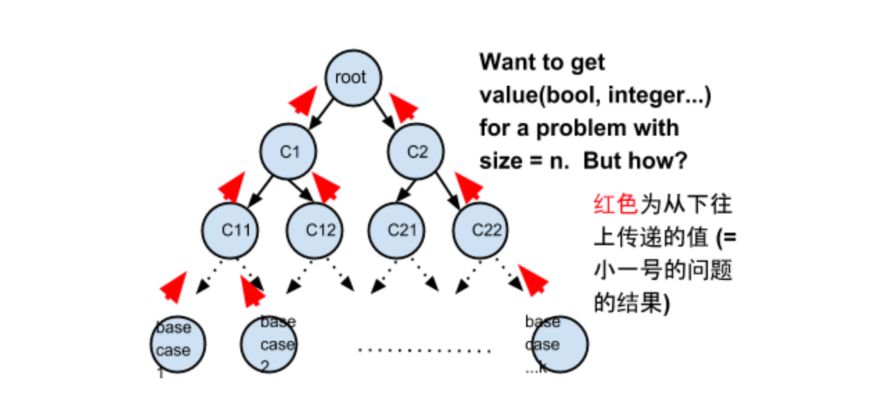
\includegraphics{source/lesson6_binarytree_recursion1.png} * Binary Tree
is the most common interviewed questions with recursion * Reasons: *
每层的node具备的性质,传递的值和下一层的性质往往一致。比较容易定义recursive
rule * Base case (generally): None under the leaf node * Example 1: int
getHeight(Node root) * Example 2: count the number of nodes in a tree *
Fundamental Knowledge: * Traversal of a binary tree * Definition *
Balanced binary tree * Complete binary tree * Binary search tree (BST)

    \paragraph{Question 2: Get Height of a binary
tree}\label{question-2-get-height-of-a-binary-tree}

\begin{verbatim}
                10 == root     4
               /  \
              5    15          3
             / \   / \ 
            2  7  12  20       2
           /
          1                    1
\end{verbatim}

\begin{figure}
\centering
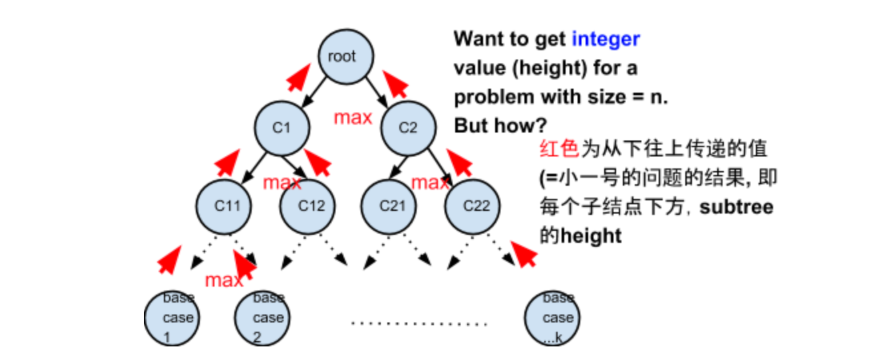
\includegraphics{source/lesson6_binarytree_recursion2.png}
\caption{Recursion}
\end{figure}

    \begin{Verbatim}[commandchars=\\\{\}]
{\color{incolor}In [{\color{incolor}29}]:} \PY{k}{class} \PY{n+nc}{Solution}\PY{p}{(}\PY{n+nb}{object}\PY{p}{)}\PY{p}{:}
             \PY{k}{def} \PY{n+nf}{get\PYZus{}height}\PY{p}{(}\PY{n+nb+bp}{self}\PY{p}{,} \PY{n}{root}\PY{p}{)}\PY{p}{:}
                 \PY{l+s+sd}{\PYZdq{}\PYZdq{}\PYZdq{}}
         \PY{l+s+sd}{        \PYZsh{} Time complexity: O(n)}
         \PY{l+s+sd}{        \PYZsh{} Space Complexity: O(h)}
         \PY{l+s+sd}{        \PYZdq{}\PYZdq{}\PYZdq{}}
                 \PY{c+c1}{\PYZsh{} Base case: child node under a leaf node}
                 \PY{k}{if} \PY{o+ow}{not} \PY{n}{root}\PY{p}{:}
                     \PY{k}{return} \PY{l+m+mi}{0}
                 
                 \PY{c+c1}{\PYZsh{} what to get from your children}
                 \PY{n}{left\PYZus{}child\PYZus{}height} \PY{o}{=} \PY{n+nb+bp}{self}\PY{o}{.}\PY{n}{get\PYZus{}height}\PY{p}{(}\PY{n}{root}\PY{o}{.}\PY{n}{left}\PY{p}{)}
                 \PY{n}{right\PYZus{}child\PYZus{}height} \PY{o}{=} \PY{n+nb+bp}{self}\PY{o}{.}\PY{n}{get\PYZus{}height}\PY{p}{(}\PY{n}{root}\PY{o}{.}\PY{n}{right}\PY{p}{)}
                 
                 \PY{c+c1}{\PYZsh{} what to do in the current stage}
                 \PY{n}{curr\PYZus{}height} \PY{o}{=} \PY{n+nb}{max}\PY{p}{(}\PY{n}{left\PYZus{}child\PYZus{}height}\PY{p}{,} \PY{n}{right\PYZus{}child\PYZus{}height}\PY{p}{)} \PY{o}{+} \PY{l+m+mi}{1}
                 
                 \PY{c+c1}{\PYZsh{} what to return to your parent}
                 \PY{k}{return} \PY{n}{curr\PYZus{}height}
         
         
         
         \PY{k}{if} \PY{n+nv+vm}{\PYZus{}\PYZus{}name\PYZus{}\PYZus{}} \PY{o}{==} \PY{l+s+s2}{\PYZdq{}}\PY{l+s+s2}{\PYZus{}\PYZus{}main\PYZus{}\PYZus{}}\PY{l+s+s2}{\PYZdq{}}\PY{p}{:}
             \PY{n}{root} \PY{o}{=} \PY{n}{TreeNode}\PY{p}{(}\PY{l+m+mi}{10}\PY{p}{)}
             \PY{n}{root}\PY{o}{.}\PY{n}{left} \PY{o}{=} \PY{n}{TreeNode}\PY{p}{(}\PY{l+m+mi}{5}\PY{p}{)}
             \PY{n}{root}\PY{o}{.}\PY{n}{right} \PY{o}{=} \PY{n}{TreeNode}\PY{p}{(}\PY{l+m+mi}{15}\PY{p}{)}
             \PY{n}{root}\PY{o}{.}\PY{n}{left}\PY{o}{.}\PY{n}{left} \PY{o}{=} \PY{n}{TreeNode}\PY{p}{(}\PY{l+m+mi}{2}\PY{p}{)}
             \PY{n}{root}\PY{o}{.}\PY{n}{left}\PY{o}{.}\PY{n}{right} \PY{o}{=} \PY{n}{TreeNode}\PY{p}{(}\PY{l+m+mi}{7}\PY{p}{)}
             \PY{n}{root}\PY{o}{.}\PY{n}{right}\PY{o}{.}\PY{n}{left} \PY{o}{=} \PY{n}{TreeNode}\PY{p}{(}\PY{l+m+mi}{12}\PY{p}{)}
             \PY{n}{root}\PY{o}{.}\PY{n}{right}\PY{o}{.}\PY{n}{right} \PY{o}{=} \PY{n}{TreeNode}\PY{p}{(}\PY{l+m+mi}{20}\PY{p}{)}
             \PY{n}{root}\PY{o}{.}\PY{n}{left}\PY{o}{.}\PY{n}{left}\PY{o}{.}\PY{n}{left} \PY{o}{=} \PY{n}{TreeNode}\PY{p}{(}\PY{l+m+mi}{1}\PY{p}{)}
         
             \PY{n}{soln} \PY{o}{=} \PY{n}{Solution}\PY{p}{(}\PY{p}{)}
             \PY{n+nb}{print}\PY{p}{(}\PY{n}{soln}\PY{o}{.}\PY{n}{get\PYZus{}height}\PY{p}{(}\PY{n}{root}\PY{p}{)}\PY{p}{)}
\end{Verbatim}


    \begin{Verbatim}[commandchars=\\\{\}]
4

    \end{Verbatim}

    Why the space complexity is \(O(h)\)?

\begin{verbatim}
                10 == root (4)     4
              /    \
            5(3)    15(2)          3
          /    \    /   \ 
       2(2)  7(1) 12(1)  20(1)     2
        /
      1(1)                         1
      / \
     N   N
\end{verbatim}

    \paragraph{Question 3: Flip Upside
Down}\label{question-3-flip-upside-down}

Given a binary tree where all the right nodes are either leaf nodes with
a sibling (a left node that shares the same parent node) or empty, flip
it upside down and turn it into a tree where the original right nodes
turned into left leaf nodes. Return the new root.

\begin{verbatim}
                1                             4
               / \                           / \
              2   3          -->            5   2
             / \                               / \
            4   5                             3   1
\end{verbatim}

Pattern: at each node,

\begin{verbatim}
               A                              B
              / \            -->             / \
             B   C                          C   A
\end{verbatim}

Recall a similar problem: \emph{reverse a linked list recursively.}

\begin{verbatim}
1 -> 2 -> [3] -> 4 -> None
         curr
1 -> 2 -> [3] <- 4
         curr.next.next = curr
         curr.next = None
\end{verbatim}

    \begin{Verbatim}[commandchars=\\\{\}]
{\color{incolor}In [{\color{incolor}30}]:} \PY{k}{class} \PY{n+nc}{Solution}\PY{p}{(}\PY{n+nb}{object}\PY{p}{)}\PY{p}{:}
             \PY{k}{def} \PY{n+nf}{flip\PYZus{}upside\PYZus{}down}\PY{p}{(}\PY{n+nb+bp}{self}\PY{p}{,} \PY{n}{root}\PY{p}{)}\PY{p}{:}
                 \PY{c+c1}{\PYZsh{} Edge case}
                 \PY{k}{if} \PY{o+ow}{not} \PY{n}{root}\PY{p}{:}
                     \PY{k}{return} \PY{n}{root}
                 
                 \PY{c+c1}{\PYZsh{} Base case: leaf node}
                 \PY{k}{if} \PY{o+ow}{not} \PY{n}{root}\PY{o}{.}\PY{n}{left} \PY{o+ow}{and} \PY{o+ow}{not} \PY{n}{root}\PY{o}{.}\PY{n}{right}\PY{p}{:}
                     \PY{k}{return} \PY{n}{root}
                 
                 \PY{c+c1}{\PYZsh{} what to get from your children}
                 \PY{n}{child\PYZus{}root} \PY{o}{=} \PY{n+nb+bp}{self}\PY{o}{.}\PY{n}{flip\PYZus{}upside\PYZus{}down}\PY{p}{(}\PY{n}{root}\PY{o}{.}\PY{n}{left}\PY{p}{)}
                 
                 \PY{c+c1}{\PYZsh{} what to do in the current stage}
                 \PY{n}{root}\PY{o}{.}\PY{n}{left}\PY{o}{.}\PY{n}{left} \PY{o}{=} \PY{n}{root}\PY{o}{.}\PY{n}{right}
                 \PY{n}{root}\PY{o}{.}\PY{n}{left}\PY{o}{.}\PY{n}{right} \PY{o}{=} \PY{n}{root}
                 \PY{n}{root}\PY{o}{.}\PY{n}{left} \PY{o}{=} \PY{k+kc}{None}
                 \PY{n}{root}\PY{o}{.}\PY{n}{right} \PY{o}{=} \PY{k+kc}{None}
                 
                 \PY{k}{return} \PY{n}{child\PYZus{}root}   
             
         \PY{k}{if} \PY{n+nv+vm}{\PYZus{}\PYZus{}name\PYZus{}\PYZus{}} \PY{o}{==} \PY{l+s+s2}{\PYZdq{}}\PY{l+s+s2}{\PYZus{}\PYZus{}main\PYZus{}\PYZus{}}\PY{l+s+s2}{\PYZdq{}}\PY{p}{:}
             \PY{n}{root} \PY{o}{=} \PY{n}{TreeNode}\PY{p}{(}\PY{l+m+mi}{1}\PY{p}{)}
             \PY{n}{root}\PY{o}{.}\PY{n}{left} \PY{o}{=} \PY{n}{TreeNode}\PY{p}{(}\PY{l+m+mi}{2}\PY{p}{)}
             \PY{n}{root}\PY{o}{.}\PY{n}{right} \PY{o}{=} \PY{n}{TreeNode}\PY{p}{(}\PY{l+m+mi}{3}\PY{p}{)}
             \PY{n}{root}\PY{o}{.}\PY{n}{left}\PY{o}{.}\PY{n}{left} \PY{o}{=} \PY{n}{TreeNode}\PY{p}{(}\PY{l+m+mi}{4}\PY{p}{)}
             \PY{n}{root}\PY{o}{.}\PY{n}{left}\PY{o}{.}\PY{n}{right} \PY{o}{=} \PY{n}{TreeNode}\PY{p}{(}\PY{l+m+mi}{5}\PY{p}{)}
             \PY{n}{traversal} \PY{o}{=} \PY{n}{Traversal}\PY{p}{(}\PY{p}{)}
             \PY{n+nb}{print}\PY{p}{(}\PY{n}{traversal}\PY{o}{.}\PY{n}{BFS\PYZus{}traversal}\PY{p}{(}\PY{n}{root}\PY{p}{)}\PY{p}{)}
         
             \PY{n}{soln} \PY{o}{=} \PY{n}{Solution}\PY{p}{(}\PY{p}{)}
             \PY{n}{new\PYZus{}root} \PY{o}{=} \PY{n}{soln}\PY{o}{.}\PY{n}{flip\PYZus{}upside\PYZus{}down}\PY{p}{(}\PY{n}{root}\PY{p}{)}
             \PY{n+nb}{print}\PY{p}{(}\PY{n}{traversal}\PY{o}{.}\PY{n}{BFS\PYZus{}traversal}\PY{p}{(}\PY{n}{new\PYZus{}root}\PY{p}{)}\PY{p}{)}
\end{Verbatim}


    \begin{Verbatim}[commandchars=\\\{\}]
[[1], [2, 3], [4, 5, '\#', '\#']]
[[4], [5, 2], ['\#', '\#', 3, 1]]

    \end{Verbatim}

    \paragraph{Question 4: For each node in a tree, store the number of
nodes in its left child
subtree}\label{question-4-for-each-node-in-a-tree-store-the-number-of-nodes-in-its-left-child-subtree}

\begin{Shaded}
\begin{Highlighting}[]
\KeywordTok{class}\NormalTok{ TreeNode:}
    \KeywordTok{def} \FunctionTok{__init__}\NormalTok{(}\VariableTok{self}\NormalTok{, x):}
        \VariableTok{self}\NormalTok{.val }\OperatorTok{=}\NormalTok{ x}
        \VariableTok{self}\NormalTok{.left }\OperatorTok{=} \VariableTok{None}
        \VariableTok{self}\NormalTok{.right }\OperatorTok{=} \VariableTok{None}
        \VariableTok{self}\NormalTok{.total_left }\OperatorTok{=}\DecValTok{0} \CommentTok{# How many nodes in its left subtree}
\end{Highlighting}
\end{Shaded}

\begin{verbatim}
                root(3)
               /      \
          node1(1)  node2 (0)
          /      \  
      node3(0)  node4(0)
\end{verbatim}

\begin{itemize}
\tightlist
\item
  Base Case: root = None -\/-\textgreater{} return 0
\item
  recursion rule:
\item
  left\_total: 左孩子的node的数目(小一号问题)
\item
  right\_total: 右孩子的node的数目(小一号问题)
\item
  root.total\_left = left\_total
\item
  return 1 + left\_total + right\_total
\end{itemize}

Way of thinking (Tricks) 1. What do you expect from your left child /
right child? (usudally it is the return type of the recursion function)
* Total number of nodes in my left subtree * Total number of nodes in my
right subtree 2. What do you want to do in the current layer? * Store
the number of nodes in the left subtree 3. What do you want to return to
your parent? (same as 1) * return total number of nodes

    \begin{Verbatim}[commandchars=\\\{\}]
{\color{incolor}In [{\color{incolor}31}]:} \PY{k}{class} \PY{n+nc}{TreeNodeEx}\PY{p}{(}\PY{n+nb}{object}\PY{p}{)}\PY{p}{:}
             \PY{k}{def} \PY{n+nf}{\PYZus{}\PYZus{}init\PYZus{}\PYZus{}}\PY{p}{(}\PY{n+nb+bp}{self}\PY{p}{,} \PY{n}{x}\PY{p}{)}\PY{p}{:}
                 \PY{n+nb+bp}{self}\PY{o}{.}\PY{n}{val} \PY{o}{=} \PY{n}{x}
                 \PY{n+nb+bp}{self}\PY{o}{.}\PY{n}{left} \PY{o}{=} \PY{k+kc}{None}
                 \PY{n+nb+bp}{self}\PY{o}{.}\PY{n}{right} \PY{o}{=} \PY{k+kc}{None}
                 \PY{n+nb+bp}{self}\PY{o}{.}\PY{n}{total\PYZus{}left} \PY{o}{=}\PY{l+m+mi}{0} \PY{c+c1}{\PYZsh{} How many nodes in its left subtree}
                 
         \PY{k}{class} \PY{n+nc}{Solution}\PY{p}{(}\PY{n+nb}{object}\PY{p}{)}\PY{p}{:}
             \PY{k}{def} \PY{n+nf}{get\PYZus{}total\PYZus{}left}\PY{p}{(}\PY{n+nb+bp}{self}\PY{p}{,} \PY{n}{root}\PY{p}{)}\PY{p}{:}
                 \PY{c+c1}{\PYZsh{} Base Case}
                 \PY{k}{if} \PY{o+ow}{not} \PY{n}{root}\PY{p}{:}
                     \PY{k}{return} \PY{l+m+mi}{0}
                 
                 \PY{c+c1}{\PYZsh{} What to get from my children?}
                 \PY{n}{left\PYZus{}child\PYZus{}nodes} \PY{o}{=} \PY{n+nb+bp}{self}\PY{o}{.}\PY{n}{get\PYZus{}total\PYZus{}left}\PY{p}{(}\PY{n}{root}\PY{o}{.}\PY{n}{left}\PY{p}{)}
                 \PY{n}{right\PYZus{}child\PYZus{}nodes} \PY{o}{=} \PY{n+nb+bp}{self}\PY{o}{.}\PY{n}{get\PYZus{}total\PYZus{}left}\PY{p}{(}\PY{n}{root}\PY{o}{.}\PY{n}{right}\PY{p}{)}
                 
                 \PY{c+c1}{\PYZsh{} What to do in the current stage}
                 \PY{n}{root}\PY{o}{.}\PY{n}{total\PYZus{}left} \PY{o}{=} \PY{n}{left\PYZus{}child\PYZus{}nodes}        
                 \PY{n}{total\PYZus{}nodes} \PY{o}{=} \PY{n}{left\PYZus{}child\PYZus{}nodes} \PY{o}{+} \PY{n}{right\PYZus{}child\PYZus{}nodes} \PY{o}{+} \PY{l+m+mi}{1}
                 
                 \PY{c+c1}{\PYZsh{} What to return to your parent        }
                 \PY{k}{return} \PY{n}{total\PYZus{}nodes}
             
         \PY{k}{if} \PY{n+nv+vm}{\PYZus{}\PYZus{}name\PYZus{}\PYZus{}} \PY{o}{==} \PY{l+s+s2}{\PYZdq{}}\PY{l+s+s2}{\PYZus{}\PYZus{}main\PYZus{}\PYZus{}}\PY{l+s+s2}{\PYZdq{}}\PY{p}{:}
             \PY{n}{root} \PY{o}{=} \PY{n}{TreeNodeEx}\PY{p}{(}\PY{l+m+mi}{3}\PY{p}{)}
             \PY{n}{root}\PY{o}{.}\PY{n}{left} \PY{o}{=} \PY{n}{TreeNodeEx}\PY{p}{(}\PY{l+m+mi}{1}\PY{p}{)}
             \PY{n}{root}\PY{o}{.}\PY{n}{right} \PY{o}{=} \PY{n}{TreeNodeEx}\PY{p}{(}\PY{l+m+mi}{2}\PY{p}{)}
             \PY{n}{root}\PY{o}{.}\PY{n}{left}\PY{o}{.}\PY{n}{left} \PY{o}{=} \PY{n}{TreeNodeEx}\PY{p}{(}\PY{l+m+mi}{4}\PY{p}{)}
             \PY{n}{root}\PY{o}{.}\PY{n}{left}\PY{o}{.}\PY{n}{right} \PY{o}{=} \PY{n}{TreeNodeEx}\PY{p}{(}\PY{l+m+mi}{5}\PY{p}{)}
             \PY{n}{traversal} \PY{o}{=} \PY{n}{Traversal}\PY{p}{(}\PY{p}{)}
             \PY{n+nb}{print}\PY{p}{(}\PY{n}{traversal}\PY{o}{.}\PY{n}{BFS\PYZus{}traversal}\PY{p}{(}\PY{n}{root}\PY{p}{)}\PY{p}{)}
         
             \PY{n}{soln} \PY{o}{=} \PY{n}{Solution}\PY{p}{(}\PY{p}{)}
             \PY{n}{soln}\PY{o}{.}\PY{n}{get\PYZus{}total\PYZus{}left}\PY{p}{(}\PY{n}{root}\PY{p}{)}
             \PY{n+nb}{print}\PY{p}{(}\PY{n}{root}\PY{o}{.}\PY{n}{total\PYZus{}left}\PY{p}{)}
\end{Verbatim}


    \begin{Verbatim}[commandchars=\\\{\}]
[[3], [1, 2], [4, 5, '\#', '\#']]
3

    \end{Verbatim}

    \paragraph{Question 5: Find the node with the max difference in the
total number of descendents in its left subtree and right
subtree}\label{question-5-find-the-node-with-the-max-difference-in-the-total-number-of-descendents-in-its-left-subtree-and-right-subtree}

\begin{verbatim}
                root(0)
               /      \
          node1(0)  node2 (2) <-- answer
          /      \        \
      node3(0)  node4(0)  node5 (1)
                              \
                            node6 (0)
\end{verbatim}

\begin{itemize}
\tightlist
\item
  Golbal variable: global\_max\_diff
\item
  Base Case: root = None -\/-\textgreater{} return 0
\item
  recursion rule:
\item
  left\_total: 左孩子的node的数目(小一号问题)
\item
  right\_total: 右孩子的node的数目(小一号问题)
\item
  diff = abs(left\_total-right\_total)
\item
  global\_max\_diff = max(diff, global\_max\_diff)
\item
  return 1 + left\_total + right\_total
\end{itemize}

Way of thinking (Tricks) 1. What do you expect from your left child /
right child? (usudally it is the return type of the recursion function)
* left\_total: total number of nodes in my left subtree * right\_total:
total number of nodes in my right subtree 2. What do you want to do in
the current layer? * diff = abs(left\_total - right\_total) *
global\_max\_diff = max(diff, global\_max\_diff) 3. What do you want to
return to your parent? (same as 1) * return total number of nodes

    \begin{Verbatim}[commandchars=\\\{\}]
{\color{incolor}In [{\color{incolor}32}]:} \PY{k}{class} \PY{n+nc}{ResultWrapper}\PY{p}{:}
             \PY{k}{def} \PY{n+nf}{\PYZus{}\PYZus{}init\PYZus{}\PYZus{}}\PY{p}{(}\PY{n+nb+bp}{self}\PY{p}{)}\PY{p}{:}
                 \PY{n+nb+bp}{self}\PY{o}{.}\PY{n}{global\PYZus{}max\PYZus{}diff} \PY{o}{=} \PY{o}{\PYZhy{}}\PY{l+m+mi}{1}
                 \PY{n+nb+bp}{self}\PY{o}{.}\PY{n}{node} \PY{o}{=} \PY{k+kc}{None}
         
         \PY{k}{class} \PY{n+nc}{Solution}\PY{p}{(}\PY{n+nb}{object}\PY{p}{)}\PY{p}{:}
             \PY{k}{def} \PY{n+nf}{get\PYZus{}max\PYZus{}diff}\PY{p}{(}\PY{n+nb+bp}{self}\PY{p}{,} \PY{n}{root}\PY{p}{)}\PY{p}{:}
                 \PY{n}{res} \PY{o}{=} \PY{n}{ResultWrapper}\PY{p}{(}\PY{p}{)}
                 \PY{n+nb+bp}{self}\PY{o}{.}\PY{n}{helper}\PY{p}{(}\PY{n}{root}\PY{p}{,} \PY{n}{res}\PY{p}{)}
                 \PY{k}{return} \PY{n}{res}\PY{o}{.}\PY{n}{node}
             
             \PY{k}{def} \PY{n+nf}{helper}\PY{p}{(}\PY{n+nb+bp}{self}\PY{p}{,} \PY{n}{root}\PY{p}{,} \PY{n}{res}\PY{p}{)}\PY{p}{:}
                 \PY{c+c1}{\PYZsh{} Base Case}
                 \PY{k}{if} \PY{o+ow}{not} \PY{n}{root}\PY{p}{:}
                     \PY{k}{return} \PY{l+m+mi}{0}
                 
                 \PY{c+c1}{\PYZsh{} What to get from my children}
                 \PY{n}{left\PYZus{}child\PYZus{}node} \PY{o}{=} \PY{n+nb+bp}{self}\PY{o}{.}\PY{n}{helper}\PY{p}{(}\PY{n}{root}\PY{o}{.}\PY{n}{left}\PY{p}{,} \PY{n}{res}\PY{p}{)}
                 \PY{n}{right\PYZus{}child\PYZus{}node} \PY{o}{=} \PY{n+nb+bp}{self}\PY{o}{.}\PY{n}{helper}\PY{p}{(}\PY{n}{root}\PY{o}{.}\PY{n}{right}\PY{p}{,} \PY{n}{res}\PY{p}{)}
                 
                 \PY{c+c1}{\PYZsh{} What to do in the current stage}
                 \PY{n}{diff} \PY{o}{=} \PY{n+nb}{abs}\PY{p}{(}\PY{n}{left\PYZus{}child\PYZus{}node} \PY{o}{\PYZhy{}} \PY{n}{right\PYZus{}child\PYZus{}node}\PY{p}{)}
                 \PY{k}{if} \PY{n}{diff} \PY{o}{\PYZgt{}} \PY{n}{res}\PY{o}{.}\PY{n}{global\PYZus{}max\PYZus{}diff}\PY{p}{:}
                     \PY{n}{res}\PY{o}{.}\PY{n}{global\PYZus{}max\PYZus{}diff} \PY{o}{=} \PY{n}{diff}
                     \PY{n}{res}\PY{o}{.}\PY{n}{node} \PY{o}{=} \PY{n}{root}
                 
                 \PY{c+c1}{\PYZsh{} What to return to my parent}
                 \PY{n}{total\PYZus{}node} \PY{o}{=} \PY{n}{left\PYZus{}child\PYZus{}node} \PY{o}{+} \PY{n}{right\PYZus{}child\PYZus{}node} \PY{o}{+} \PY{l+m+mi}{1}
                 \PY{k}{return} \PY{n}{total\PYZus{}node}
             
         \PY{k}{if} \PY{n+nv+vm}{\PYZus{}\PYZus{}name\PYZus{}\PYZus{}} \PY{o}{==} \PY{l+s+s2}{\PYZdq{}}\PY{l+s+s2}{\PYZus{}\PYZus{}main\PYZus{}\PYZus{}}\PY{l+s+s2}{\PYZdq{}}\PY{p}{:}
             \PY{n}{root} \PY{o}{=} \PY{n}{TreeNode}\PY{p}{(}\PY{l+m+mi}{0}\PY{p}{)}
             \PY{n}{root}\PY{o}{.}\PY{n}{left} \PY{o}{=} \PY{n}{TreeNode}\PY{p}{(}\PY{l+m+mi}{1}\PY{p}{)}
             \PY{n}{root}\PY{o}{.}\PY{n}{left}\PY{o}{.}\PY{n}{left} \PY{o}{=} \PY{n}{TreeNode}\PY{p}{(}\PY{l+m+mi}{3}\PY{p}{)}
             \PY{n}{root}\PY{o}{.}\PY{n}{left}\PY{o}{.}\PY{n}{right} \PY{o}{=} \PY{n}{TreeNode}\PY{p}{(}\PY{l+m+mi}{4}\PY{p}{)}
             \PY{n}{root}\PY{o}{.}\PY{n}{right} \PY{o}{=} \PY{n}{TreeNode}\PY{p}{(}\PY{l+m+mi}{2}\PY{p}{)}
             \PY{n}{root}\PY{o}{.}\PY{n}{right}\PY{o}{.}\PY{n}{right} \PY{o}{=} \PY{n}{TreeNode}\PY{p}{(}\PY{l+m+mi}{5}\PY{p}{)}
             \PY{n}{root}\PY{o}{.}\PY{n}{right}\PY{o}{.}\PY{n}{right}\PY{o}{.}\PY{n}{right} \PY{o}{=} \PY{n}{TreeNode}\PY{p}{(}\PY{l+m+mi}{6}\PY{p}{)}
             \PY{n}{traversal} \PY{o}{=} \PY{n}{Traversal}\PY{p}{(}\PY{p}{)}
             \PY{n+nb}{print}\PY{p}{(}\PY{n}{traversal}\PY{o}{.}\PY{n}{BFS\PYZus{}traversal}\PY{p}{(}\PY{n}{root}\PY{p}{)}\PY{p}{)}
         
             \PY{n}{soln} \PY{o}{=} \PY{n}{Solution}\PY{p}{(}\PY{p}{)}
             \PY{n}{node} \PY{o}{=} \PY{n}{soln}\PY{o}{.}\PY{n}{get\PYZus{}max\PYZus{}diff}\PY{p}{(}\PY{n}{root}\PY{p}{)}
             \PY{n+nb}{print}\PY{p}{(}\PY{n}{node}\PY{o}{.}\PY{n}{val}\PY{p}{)}
\end{Verbatim}


    \begin{Verbatim}[commandchars=\\\{\}]
[[0], [1, 2], [3, 4, '\#', 5], ['\#', '\#', '\#', '\#', '\#', 6]]
2

    \end{Verbatim}

    \begin{Verbatim}[commandchars=\\\{\}]
{\color{incolor}In [{\color{incolor}33}]:} \PY{k}{class} \PY{n+nc}{Solution}\PY{p}{(}\PY{n+nb}{object}\PY{p}{)}\PY{p}{:}
             \PY{k}{def} \PY{n+nf}{get\PYZus{}max\PYZus{}diff}\PY{p}{(}\PY{n+nb+bp}{self}\PY{p}{,} \PY{n}{root}\PY{p}{)}\PY{p}{:}
                 \PY{n}{res} \PY{o}{=} \PY{p}{[}\PY{k+kc}{None}\PY{p}{,} \PY{o}{\PYZhy{}}\PY{l+m+mi}{1}\PY{p}{]}  \PY{c+c1}{\PYZsh{} node, max\PYZus{}diff }
                 \PY{n+nb+bp}{self}\PY{o}{.}\PY{n}{helper}\PY{p}{(}\PY{n}{root}\PY{p}{,} \PY{n}{res}\PY{p}{)}
                 \PY{k}{return} \PY{n}{res}\PY{p}{[}\PY{l+m+mi}{0}\PY{p}{]}
             
             \PY{k}{def} \PY{n+nf}{helper}\PY{p}{(}\PY{n+nb+bp}{self}\PY{p}{,} \PY{n}{root}\PY{p}{,} \PY{n}{res}\PY{p}{)}\PY{p}{:}
                 \PY{c+c1}{\PYZsh{} Base Case}
                 \PY{k}{if} \PY{o+ow}{not} \PY{n}{root}\PY{p}{:}
                     \PY{k}{return} \PY{l+m+mi}{0}
                 
                 \PY{c+c1}{\PYZsh{} What to get from my children}
                 \PY{n}{left\PYZus{}child\PYZus{}node} \PY{o}{=} \PY{n+nb+bp}{self}\PY{o}{.}\PY{n}{helper}\PY{p}{(}\PY{n}{root}\PY{o}{.}\PY{n}{left}\PY{p}{,} \PY{n}{res}\PY{p}{)}
                 \PY{n}{right\PYZus{}child\PYZus{}node} \PY{o}{=} \PY{n+nb+bp}{self}\PY{o}{.}\PY{n}{helper}\PY{p}{(}\PY{n}{root}\PY{o}{.}\PY{n}{right}\PY{p}{,} \PY{n}{res}\PY{p}{)}
                 
                 \PY{c+c1}{\PYZsh{} What to do in the current stage}
                 \PY{n}{diff} \PY{o}{=} \PY{n+nb}{abs}\PY{p}{(}\PY{n}{left\PYZus{}child\PYZus{}node} \PY{o}{\PYZhy{}} \PY{n}{right\PYZus{}child\PYZus{}node}\PY{p}{)}
                 \PY{k}{if} \PY{n}{diff} \PY{o}{\PYZgt{}} \PY{n}{res}\PY{p}{[}\PY{l+m+mi}{1}\PY{p}{]}\PY{p}{:}
                     \PY{n}{res}\PY{p}{[}\PY{l+m+mi}{1}\PY{p}{]} \PY{o}{=} \PY{n}{diff}
                     \PY{n}{res}\PY{p}{[}\PY{l+m+mi}{0}\PY{p}{]} \PY{o}{=} \PY{n}{root}
                 
                 \PY{c+c1}{\PYZsh{} What to return to my parent}
                 \PY{n}{total\PYZus{}node} \PY{o}{=} \PY{n}{left\PYZus{}child\PYZus{}node} \PY{o}{+} \PY{n}{right\PYZus{}child\PYZus{}node} \PY{o}{+} \PY{l+m+mi}{1}
                 \PY{k}{return} \PY{n}{total\PYZus{}node}
             
         \PY{k}{if} \PY{n+nv+vm}{\PYZus{}\PYZus{}name\PYZus{}\PYZus{}} \PY{o}{==} \PY{l+s+s2}{\PYZdq{}}\PY{l+s+s2}{\PYZus{}\PYZus{}main\PYZus{}\PYZus{}}\PY{l+s+s2}{\PYZdq{}}\PY{p}{:}
             \PY{n}{root} \PY{o}{=} \PY{n}{TreeNode}\PY{p}{(}\PY{l+m+mi}{0}\PY{p}{)}
             \PY{n}{root}\PY{o}{.}\PY{n}{left} \PY{o}{=} \PY{n}{TreeNode}\PY{p}{(}\PY{l+m+mi}{1}\PY{p}{)}
             \PY{n}{root}\PY{o}{.}\PY{n}{left}\PY{o}{.}\PY{n}{left} \PY{o}{=} \PY{n}{TreeNode}\PY{p}{(}\PY{l+m+mi}{3}\PY{p}{)}
             \PY{n}{root}\PY{o}{.}\PY{n}{left}\PY{o}{.}\PY{n}{right} \PY{o}{=} \PY{n}{TreeNode}\PY{p}{(}\PY{l+m+mi}{4}\PY{p}{)}
             \PY{n}{root}\PY{o}{.}\PY{n}{right} \PY{o}{=} \PY{n}{TreeNode}\PY{p}{(}\PY{l+m+mi}{2}\PY{p}{)}
             \PY{n}{root}\PY{o}{.}\PY{n}{right}\PY{o}{.}\PY{n}{right} \PY{o}{=} \PY{n}{TreeNode}\PY{p}{(}\PY{l+m+mi}{5}\PY{p}{)}
             \PY{n}{root}\PY{o}{.}\PY{n}{right}\PY{o}{.}\PY{n}{right}\PY{o}{.}\PY{n}{right} \PY{o}{=} \PY{n}{TreeNode}\PY{p}{(}\PY{l+m+mi}{6}\PY{p}{)}
             \PY{n}{traversal} \PY{o}{=} \PY{n}{Traversal}\PY{p}{(}\PY{p}{)}
             \PY{n+nb}{print}\PY{p}{(}\PY{n}{traversal}\PY{o}{.}\PY{n}{BFS\PYZus{}traversal}\PY{p}{(}\PY{n}{root}\PY{p}{)}\PY{p}{)}
         
             \PY{n}{soln} \PY{o}{=} \PY{n}{Solution}\PY{p}{(}\PY{p}{)}
             \PY{n}{node} \PY{o}{=} \PY{n}{soln}\PY{o}{.}\PY{n}{get\PYZus{}max\PYZus{}diff}\PY{p}{(}\PY{n}{root}\PY{p}{)}
             \PY{n+nb}{print}\PY{p}{(}\PY{n}{node}\PY{o}{.}\PY{n}{val}\PY{p}{)}
\end{Verbatim}


    \begin{Verbatim}[commandchars=\\\{\}]
[[0], [1, 2], [3, 4, '\#', 5], ['\#', '\#', '\#', '\#', '\#', 6]]
2

    \end{Verbatim}

    How to choose Base Case?\\
Generally, choose root is None as base case. But sometimes, if we need
someting related to leaf, we need to choose leaf node (root.left is None
and root.right is None) as base case.

    \paragraph{Question 6: Given a binary tree, find its minimum
depth.}\label{question-6-given-a-binary-tree-find-its-minimum-depth.}

The minimum depth is the number of nodes along the shortest path from
the root node down to the nearest \textbf{leaf node}.

Leaf node: has no left child and no right child.

\begin{verbatim}
           root(2)                             root(4)  <-- not a leaf node
          /      \                            /      \
     node1(1)  node2(3)     Edge case -->  None     node2(3)  <-- not a leaf node
                    \                              /     \
                  node3(2)                       None node3(2)
                   /      \                            /      \
                node4(1)  node5(1)                  node4(1)  node5(1)  <-- Base case
\end{verbatim}

\emph{Wrong Solution}: choose root is None as base case

If we choose root is None as base case, then we cannot determine whether
its parent is a leaf node or not.

For some nodes, they only have a child. Their minimum height should be
determined by their real child not by a non-existing child.

\emph{Correct Solution}: Choose leaf (root.left is None and root.right
is None) as base case

    \begin{Verbatim}[commandchars=\\\{\}]
{\color{incolor}In [{\color{incolor}34}]:} \PY{k}{class} \PY{n+nc}{Solution}\PY{p}{(}\PY{n+nb}{object}\PY{p}{)}\PY{p}{:}
             \PY{k}{def} \PY{n+nf}{get\PYZus{}minimum\PYZus{}depth\PYZus{}wrong}\PY{p}{(}\PY{n+nb+bp}{self}\PY{p}{,} \PY{n}{root}\PY{p}{)}\PY{p}{:}
                 \PY{c+c1}{\PYZsh{} Base case}
                 \PY{k}{if} \PY{n}{root} \PY{o+ow}{is} \PY{k+kc}{None}\PY{p}{:}
                     \PY{k}{return} \PY{l+m+mi}{0}
                 
                 \PY{n}{left\PYZus{}minimum\PYZus{}depth} \PY{o}{=} \PY{n+nb+bp}{self}\PY{o}{.}\PY{n}{get\PYZus{}minimum\PYZus{}depth\PYZus{}wrong}\PY{p}{(}\PY{n}{root}\PY{o}{.}\PY{n}{left}\PY{p}{)} 
                 \PY{n}{right\PYZus{}minimum\PYZus{}depth} \PY{o}{=} \PY{n+nb+bp}{self}\PY{o}{.}\PY{n}{get\PYZus{}minimum\PYZus{}depth\PYZus{}wrong}\PY{p}{(}\PY{n}{root}\PY{o}{.}\PY{n}{right}\PY{p}{)}
                 
                 \PY{n}{curr\PYZus{}minimum\PYZus{}depth} \PY{o}{=} \PY{n+nb}{min}\PY{p}{(}\PY{n}{left\PYZus{}minimum\PYZus{}depth}\PY{p}{,} \PY{n}{right\PYZus{}minimum\PYZus{}depth}\PY{p}{)} \PY{o}{+} \PY{l+m+mi}{1}
                 \PY{k}{return} \PY{n}{curr\PYZus{}minimum\PYZus{}depth}
             
             \PY{k}{def} \PY{n+nf}{get\PYZus{}minimum\PYZus{}depth}\PY{p}{(}\PY{n+nb+bp}{self}\PY{p}{,} \PY{n}{root}\PY{p}{)}\PY{p}{:}
                 \PY{c+c1}{\PYZsh{} Edge case, just to handle root is None}
                 \PY{k}{if} \PY{n}{root} \PY{o+ow}{is} \PY{k+kc}{None}\PY{p}{:}
                     \PY{k}{return} \PY{l+m+mi}{0}
                 \PY{c+c1}{\PYZsh{} Base case, leaf node}
                 \PY{k}{if} \PY{n}{root}\PY{o}{.}\PY{n}{left} \PY{o+ow}{is} \PY{k+kc}{None} \PY{o+ow}{and} \PY{n}{root}\PY{o}{.}\PY{n}{right} \PY{o+ow}{is} \PY{k+kc}{None}\PY{p}{:}
                     \PY{k}{return} \PY{l+m+mi}{1}
                 
                 \PY{n}{left\PYZus{}minimum\PYZus{}depth} \PY{o}{=} \PY{n+nb+bp}{self}\PY{o}{.}\PY{n}{get\PYZus{}minimum\PYZus{}depth}\PY{p}{(}\PY{n}{root}\PY{o}{.}\PY{n}{left}\PY{p}{)} \PY{k}{if} \PY{n}{root}\PY{o}{.}\PY{n}{left} \PY{o+ow}{is} \PY{o+ow}{not} \PY{k+kc}{None} \PY{k}{else} \PY{n+nb}{float}\PY{p}{(}\PY{l+s+s1}{\PYZsq{}}\PY{l+s+s1}{inf}\PY{l+s+s1}{\PYZsq{}}\PY{p}{)}
                 \PY{n}{right\PYZus{}minimum\PYZus{}depth} \PY{o}{=} \PY{n+nb+bp}{self}\PY{o}{.}\PY{n}{get\PYZus{}minimum\PYZus{}depth}\PY{p}{(}\PY{n}{root}\PY{o}{.}\PY{n}{right}\PY{p}{)} \PY{k}{if} \PY{n}{root}\PY{o}{.}\PY{n}{right} \PY{o+ow}{is} \PY{o+ow}{not} \PY{k+kc}{None} \PY{k}{else} \PY{n+nb}{float}\PY{p}{(}\PY{l+s+s1}{\PYZsq{}}\PY{l+s+s1}{inf}\PY{l+s+s1}{\PYZsq{}}\PY{p}{)}
                 
                 \PY{n}{curr\PYZus{}minimum\PYZus{}depth} \PY{o}{=} \PY{n+nb}{min}\PY{p}{(}\PY{n}{left\PYZus{}minimum\PYZus{}depth}\PY{p}{,} \PY{n}{right\PYZus{}minimum\PYZus{}depth}\PY{p}{)} \PY{o}{+} \PY{l+m+mi}{1}
                 \PY{k}{return} \PY{n}{curr\PYZus{}minimum\PYZus{}depth}
             
         \PY{k}{if} \PY{n+nv+vm}{\PYZus{}\PYZus{}name\PYZus{}\PYZus{}} \PY{o}{==} \PY{l+s+s2}{\PYZdq{}}\PY{l+s+s2}{\PYZus{}\PYZus{}main\PYZus{}\PYZus{}}\PY{l+s+s2}{\PYZdq{}}\PY{p}{:}
             \PY{n}{root} \PY{o}{=} \PY{n}{TreeNode}\PY{p}{(}\PY{l+m+mi}{0}\PY{p}{)}
             \PY{n}{root}\PY{o}{.}\PY{n}{left} \PY{o}{=} \PY{n}{TreeNode}\PY{p}{(}\PY{l+m+mi}{1}\PY{p}{)}
             \PY{n}{root}\PY{o}{.}\PY{n}{right} \PY{o}{=} \PY{n}{TreeNode}\PY{p}{(}\PY{l+m+mi}{2}\PY{p}{)}
             \PY{n}{root}\PY{o}{.}\PY{n}{right}\PY{o}{.}\PY{n}{right} \PY{o}{=} \PY{n}{TreeNode}\PY{p}{(}\PY{l+m+mi}{3}\PY{p}{)}
             \PY{n}{root}\PY{o}{.}\PY{n}{right}\PY{o}{.}\PY{n}{right}\PY{o}{.}\PY{n}{left} \PY{o}{=} \PY{n}{TreeNode}\PY{p}{(}\PY{l+m+mi}{4}\PY{p}{)}
             \PY{n}{root}\PY{o}{.}\PY{n}{right}\PY{o}{.}\PY{n}{right}\PY{o}{.}\PY{n}{right} \PY{o}{=} \PY{n}{TreeNode}\PY{p}{(}\PY{l+m+mi}{5}\PY{p}{)}
             \PY{n}{traversal} \PY{o}{=} \PY{n}{Traversal}\PY{p}{(}\PY{p}{)}
             \PY{n+nb}{print}\PY{p}{(}\PY{n}{traversal}\PY{o}{.}\PY{n}{BFS\PYZus{}traversal}\PY{p}{(}\PY{n}{root}\PY{p}{)}\PY{p}{)}
         
             \PY{n}{soln} \PY{o}{=} \PY{n}{Solution}\PY{p}{(}\PY{p}{)}
             \PY{n+nb}{print}\PY{p}{(}\PY{n}{soln}\PY{o}{.}\PY{n}{get\PYZus{}minimum\PYZus{}depth\PYZus{}wrong}\PY{p}{(}\PY{n}{root}\PY{p}{)}\PY{p}{)}
             \PY{n+nb}{print}\PY{p}{(}\PY{n}{soln}\PY{o}{.}\PY{n}{get\PYZus{}minimum\PYZus{}depth}\PY{p}{(}\PY{n}{root}\PY{p}{)}\PY{p}{)}
         
             \PY{n}{root} \PY{o}{=} \PY{n}{TreeNode}\PY{p}{(}\PY{l+m+mi}{0}\PY{p}{)}
             \PY{n}{root}\PY{o}{.}\PY{n}{right} \PY{o}{=} \PY{n}{TreeNode}\PY{p}{(}\PY{l+m+mi}{2}\PY{p}{)}
             \PY{n}{root}\PY{o}{.}\PY{n}{right}\PY{o}{.}\PY{n}{right} \PY{o}{=} \PY{n}{TreeNode}\PY{p}{(}\PY{l+m+mi}{3}\PY{p}{)}
             \PY{n}{root}\PY{o}{.}\PY{n}{right}\PY{o}{.}\PY{n}{right}\PY{o}{.}\PY{n}{left} \PY{o}{=} \PY{n}{TreeNode}\PY{p}{(}\PY{l+m+mi}{4}\PY{p}{)}
             \PY{n}{root}\PY{o}{.}\PY{n}{right}\PY{o}{.}\PY{n}{right}\PY{o}{.}\PY{n}{right} \PY{o}{=} \PY{n}{TreeNode}\PY{p}{(}\PY{l+m+mi}{5}\PY{p}{)}
             \PY{n}{traversal} \PY{o}{=} \PY{n}{Traversal}\PY{p}{(}\PY{p}{)}
             \PY{n+nb}{print}\PY{p}{(}\PY{n}{traversal}\PY{o}{.}\PY{n}{BFS\PYZus{}traversal}\PY{p}{(}\PY{n}{root}\PY{p}{)}\PY{p}{)}
         
             \PY{n}{soln} \PY{o}{=} \PY{n}{Solution}\PY{p}{(}\PY{p}{)}
             \PY{n+nb}{print}\PY{p}{(}\PY{n}{soln}\PY{o}{.}\PY{n}{get\PYZus{}minimum\PYZus{}depth\PYZus{}wrong}\PY{p}{(}\PY{n}{root}\PY{p}{)}\PY{p}{)}
             \PY{n+nb}{print}\PY{p}{(}\PY{n}{soln}\PY{o}{.}\PY{n}{get\PYZus{}minimum\PYZus{}depth}\PY{p}{(}\PY{n}{root}\PY{p}{)}\PY{p}{)}
\end{Verbatim}


    \begin{Verbatim}[commandchars=\\\{\}]
[[0], [1, 2], ['\#', '\#', '\#', 3], [4, 5]]
2
2
[[0], ['\#', 2], ['\#', 3], [4, 5]]
1
4

    \end{Verbatim}

    \paragraph{Question 6.1: {[}Lintcode 97{]} {[}Maximum Depth of Binary
Tree{]}(https://www.lintcode.com/problem/maximum-depth-of-binary-tree/description)}\label{question-6.1-lintcode-97-maximum-depth-of-binary-treehttpswww.lintcode.comproblemmaximum-depth-of-binary-treedescription}

Given a binary tree, find its maximum depth.

The maximum depth is the number of nodes along the longest path from the
root node down to the farthest leaf node.

Example 1:

\begin{verbatim}
Input: tree = {}
Output: 0
Explanation: The height of empty tree is 0.
\end{verbatim}

Example 2:

\begin{verbatim}
Input: tree = {1,2,3,#,#,4,5}
Output: 3   
Explanation: Like this:
   1
  / \                
 2   3                
    / \                
   4   5
it will be serialized {1,2,3,#,#,4,5}
\end{verbatim}

    \begin{Verbatim}[commandchars=\\\{\}]
{\color{incolor}In [{\color{incolor}80}]:} \PY{k}{class} \PY{n+nc}{Solution}\PY{p}{(}\PY{n+nb}{object}\PY{p}{)}\PY{p}{:}    
             \PY{k}{def} \PY{n+nf}{get\PYZus{}maximum\PYZus{}depth}\PY{p}{(}\PY{n+nb+bp}{self}\PY{p}{,} \PY{n}{root}\PY{p}{)}\PY{p}{:}
                 \PY{c+c1}{\PYZsh{} Edge case, just to handle root is None}
                 \PY{k}{if} \PY{n}{root} \PY{o+ow}{is} \PY{k+kc}{None}\PY{p}{:}
                     \PY{k}{return} \PY{l+m+mi}{0}
                 \PY{c+c1}{\PYZsh{} Base case, leaf node}
                 \PY{k}{if} \PY{n}{root}\PY{o}{.}\PY{n}{left} \PY{o+ow}{is} \PY{k+kc}{None} \PY{o+ow}{and} \PY{n}{root}\PY{o}{.}\PY{n}{right} \PY{o+ow}{is} \PY{k+kc}{None}\PY{p}{:}
                     \PY{k}{return} \PY{l+m+mi}{1}
                 
                 \PY{n}{left\PYZus{}maximum\PYZus{}depth} \PY{o}{=} \PY{n+nb+bp}{self}\PY{o}{.}\PY{n}{get\PYZus{}maximum\PYZus{}depth}\PY{p}{(}\PY{n}{root}\PY{o}{.}\PY{n}{left}\PY{p}{)} \PY{k}{if} \PY{n}{root}\PY{o}{.}\PY{n}{left} \PY{o+ow}{is} \PY{o+ow}{not} \PY{k+kc}{None} \PY{k}{else} \PY{l+m+mi}{0}
                 \PY{n}{right\PYZus{}maximum\PYZus{}depth} \PY{o}{=} \PY{n+nb+bp}{self}\PY{o}{.}\PY{n}{get\PYZus{}maximum\PYZus{}depth}\PY{p}{(}\PY{n}{root}\PY{o}{.}\PY{n}{right}\PY{p}{)} \PY{k}{if} \PY{n}{root}\PY{o}{.}\PY{n}{right} \PY{o+ow}{is} \PY{o+ow}{not} \PY{k+kc}{None} \PY{k}{else} \PY{l+m+mi}{0}
                 
                 \PY{n}{curr\PYZus{}maximum\PYZus{}depth} \PY{o}{=} \PY{n+nb}{max}\PY{p}{(}\PY{n}{left\PYZus{}maximum\PYZus{}depth}\PY{p}{,} \PY{n}{right\PYZus{}maximum\PYZus{}depth}\PY{p}{)} \PY{o}{+} \PY{l+m+mi}{1}
                 \PY{k}{return} \PY{n}{curr\PYZus{}maximum\PYZus{}depth}
             
         \PY{k}{if} \PY{n+nv+vm}{\PYZus{}\PYZus{}name\PYZus{}\PYZus{}} \PY{o}{==} \PY{l+s+s2}{\PYZdq{}}\PY{l+s+s2}{\PYZus{}\PYZus{}main\PYZus{}\PYZus{}}\PY{l+s+s2}{\PYZdq{}}\PY{p}{:}
             \PY{n}{root} \PY{o}{=} \PY{n}{TreeNode}\PY{p}{(}\PY{l+m+mi}{0}\PY{p}{)}
             \PY{n}{root}\PY{o}{.}\PY{n}{left} \PY{o}{=} \PY{n}{TreeNode}\PY{p}{(}\PY{l+m+mi}{1}\PY{p}{)}
             \PY{n}{root}\PY{o}{.}\PY{n}{right} \PY{o}{=} \PY{n}{TreeNode}\PY{p}{(}\PY{l+m+mi}{2}\PY{p}{)}
             \PY{n}{root}\PY{o}{.}\PY{n}{right}\PY{o}{.}\PY{n}{right} \PY{o}{=} \PY{n}{TreeNode}\PY{p}{(}\PY{l+m+mi}{3}\PY{p}{)}
             \PY{n}{root}\PY{o}{.}\PY{n}{right}\PY{o}{.}\PY{n}{right}\PY{o}{.}\PY{n}{left} \PY{o}{=} \PY{n}{TreeNode}\PY{p}{(}\PY{l+m+mi}{4}\PY{p}{)}
             \PY{n}{root}\PY{o}{.}\PY{n}{right}\PY{o}{.}\PY{n}{right}\PY{o}{.}\PY{n}{right} \PY{o}{=} \PY{n}{TreeNode}\PY{p}{(}\PY{l+m+mi}{5}\PY{p}{)}
             \PY{n}{traversal} \PY{o}{=} \PY{n}{Traversal}\PY{p}{(}\PY{p}{)}
             \PY{n+nb}{print}\PY{p}{(}\PY{n}{traversal}\PY{o}{.}\PY{n}{BFS\PYZus{}traversal}\PY{p}{(}\PY{n}{root}\PY{p}{)}\PY{p}{)}
         
             \PY{n}{soln} \PY{o}{=} \PY{n}{Solution}\PY{p}{(}\PY{p}{)}
             \PY{n+nb}{print}\PY{p}{(}\PY{n}{soln}\PY{o}{.}\PY{n}{get\PYZus{}maximum\PYZus{}depth}\PY{p}{(}\PY{n}{root}\PY{p}{)}\PY{p}{)}
         
             \PY{n}{root} \PY{o}{=} \PY{n}{TreeNode}\PY{p}{(}\PY{l+m+mi}{0}\PY{p}{)}
             \PY{n}{root}\PY{o}{.}\PY{n}{right} \PY{o}{=} \PY{n}{TreeNode}\PY{p}{(}\PY{l+m+mi}{2}\PY{p}{)}
             \PY{n}{root}\PY{o}{.}\PY{n}{right}\PY{o}{.}\PY{n}{right} \PY{o}{=} \PY{n}{TreeNode}\PY{p}{(}\PY{l+m+mi}{3}\PY{p}{)}
             \PY{n}{root}\PY{o}{.}\PY{n}{right}\PY{o}{.}\PY{n}{right}\PY{o}{.}\PY{n}{left} \PY{o}{=} \PY{n}{TreeNode}\PY{p}{(}\PY{l+m+mi}{4}\PY{p}{)}
             \PY{n}{root}\PY{o}{.}\PY{n}{right}\PY{o}{.}\PY{n}{right}\PY{o}{.}\PY{n}{right} \PY{o}{=} \PY{n}{TreeNode}\PY{p}{(}\PY{l+m+mi}{5}\PY{p}{)}
             \PY{n}{traversal} \PY{o}{=} \PY{n}{Traversal}\PY{p}{(}\PY{p}{)}
             \PY{n+nb}{print}\PY{p}{(}\PY{n}{traversal}\PY{o}{.}\PY{n}{BFS\PYZus{}traversal}\PY{p}{(}\PY{n}{root}\PY{p}{)}\PY{p}{)}
         
             \PY{n}{soln} \PY{o}{=} \PY{n}{Solution}\PY{p}{(}\PY{p}{)}
             \PY{n+nb}{print}\PY{p}{(}\PY{n}{soln}\PY{o}{.}\PY{n}{get\PYZus{}maximum\PYZus{}depth}\PY{p}{(}\PY{n}{root}\PY{p}{)}\PY{p}{)}
\end{Verbatim}


    \begin{Verbatim}[commandchars=\\\{\}]
[[0], [1, 2], ['\#', '\#', '\#', 3], [4, 5]]
4
[[0], ['\#', 2], ['\#', 3], [4, 5]]
4

    \end{Verbatim}

    \paragraph{Question 7: {[}Leetcode 298{]} Binary Tree Longest
Consecutive
Sequence}\label{question-7-leetcode-298-binary-tree-longest-consecutive-sequence}

Given a binary tree, find the length of the longest consecutive sequence
path. The path refers to any sequence of nodes from some starting node
to any node in the tree along the parent-child connections. The longest
consecutive path needs to be from parent to child (cannot be the
reverse).

Example 1:

\begin{verbatim}
Input:
   1
    \
     3
    / \
   2   4
        \
         5
Output:3
Explanation:
Longest consecutive sequence path is 3-4-5, so return 3.
\end{verbatim}

Example 2:

\begin{verbatim}
Input:
   2
    \
     3
    / 
   2    
  / 
 1
Output:2
Explanation:
Longest consecutive sequence path is 2-3,not 3-2-1, so return 2.
\end{verbatim}

    \begin{Verbatim}[commandchars=\\\{\}]
{\color{incolor}In [{\color{incolor}35}]:} \PY{k}{class} \PY{n+nc}{Solution}\PY{p}{(}\PY{n+nb}{object}\PY{p}{)}\PY{p}{:}
             \PY{k}{def} \PY{n+nf}{get\PYZus{}longest}\PY{p}{(}\PY{n+nb+bp}{self}\PY{p}{,} \PY{n}{root}\PY{p}{)}\PY{p}{:}
                 \PY{l+s+sd}{\PYZdq{}\PYZdq{}\PYZdq{}}
         \PY{l+s+sd}{        \PYZsh{} Time Complexity: O(n)}
         \PY{l+s+sd}{        \PYZsh{} Space Complexity: O(h)}
         \PY{l+s+sd}{        \PYZdq{}\PYZdq{}\PYZdq{}}
                 \PY{k}{return} \PY{n+nb+bp}{self}\PY{o}{.}\PY{n}{longest}\PY{p}{(}\PY{n}{root}\PY{p}{,} \PY{k+kc}{None}\PY{p}{,} \PY{l+m+mi}{0}\PY{p}{)}
         
             \PY{k}{def} \PY{n+nf}{longest}\PY{p}{(}\PY{n+nb+bp}{self}\PY{p}{,} \PY{n}{curr}\PY{p}{,} \PY{n}{parent}\PY{p}{,} \PY{n}{parent\PYZus{}len}\PY{p}{)}\PY{p}{:}
                 \PY{c+c1}{\PYZsh{} Base Case}
                 \PY{k}{if} \PY{o+ow}{not} \PY{n}{curr}\PY{p}{:}
                     \PY{k}{return} \PY{n}{parent\PYZus{}len}
         
                 \PY{c+c1}{\PYZsh{} What to do in the current stage}
                 \PY{n}{curr\PYZus{}len} \PY{o}{=} \PY{l+m+mi}{1}
                 \PY{k}{if} \PY{n}{parent} \PY{o+ow}{and} \PY{n}{curr}\PY{o}{.}\PY{n}{val} \PY{o}{==} \PY{n}{parent}\PY{o}{.}\PY{n}{val} \PY{o}{+} \PY{l+m+mi}{1}\PY{p}{:}
                     \PY{n}{curr\PYZus{}len} \PY{o}{=} \PY{n}{parent\PYZus{}len} \PY{o}{+} \PY{l+m+mi}{1}
         
                 \PY{c+c1}{\PYZsh{} What to get from your children}
                 \PY{n}{left\PYZus{}len} \PY{o}{=} \PY{n+nb+bp}{self}\PY{o}{.}\PY{n}{longest}\PY{p}{(}\PY{n}{curr}\PY{o}{.}\PY{n}{left}\PY{p}{,} \PY{n}{curr}\PY{p}{,} \PY{n}{curr\PYZus{}len}\PY{p}{)}
                 \PY{n}{right\PYZus{}len} \PY{o}{=} \PY{n+nb+bp}{self}\PY{o}{.}\PY{n}{longest}\PY{p}{(}\PY{n}{curr}\PY{o}{.}\PY{n}{right}\PY{p}{,} \PY{n}{curr}\PY{p}{,} \PY{n}{curr\PYZus{}len}\PY{p}{)}
         
                 \PY{c+c1}{\PYZsh{} What to return to your parent}
                 \PY{k}{return} \PY{n+nb}{max}\PY{p}{(}\PY{n}{parent\PYZus{}len}\PY{p}{,} \PY{n}{left\PYZus{}len}\PY{p}{,} \PY{n}{right\PYZus{}len}\PY{p}{)}
         
         \PY{k}{if} \PY{n+nv+vm}{\PYZus{}\PYZus{}name\PYZus{}\PYZus{}} \PY{o}{==} \PY{l+s+s2}{\PYZdq{}}\PY{l+s+s2}{\PYZus{}\PYZus{}main\PYZus{}\PYZus{}}\PY{l+s+s2}{\PYZdq{}}\PY{p}{:}
             \PY{n}{root} \PY{o}{=} \PY{n}{TreeNode}\PY{p}{(}\PY{l+m+mi}{1}\PY{p}{)}
             \PY{n}{root}\PY{o}{.}\PY{n}{right} \PY{o}{=} \PY{n}{TreeNode}\PY{p}{(}\PY{l+m+mi}{3}\PY{p}{)}
             \PY{n}{root}\PY{o}{.}\PY{n}{right}\PY{o}{.}\PY{n}{left} \PY{o}{=} \PY{n}{TreeNode}\PY{p}{(}\PY{l+m+mi}{2}\PY{p}{)}
             \PY{n}{root}\PY{o}{.}\PY{n}{right}\PY{o}{.}\PY{n}{right} \PY{o}{=} \PY{n}{TreeNode}\PY{p}{(}\PY{l+m+mi}{4}\PY{p}{)}
             \PY{n}{root}\PY{o}{.}\PY{n}{right}\PY{o}{.}\PY{n}{right}\PY{o}{.}\PY{n}{right} \PY{o}{=} \PY{n}{TreeNode}\PY{p}{(}\PY{l+m+mi}{5}\PY{p}{)}
         
             \PY{n}{soln} \PY{o}{=} \PY{n}{Solution}\PY{p}{(}\PY{p}{)}
             \PY{n+nb}{print}\PY{p}{(}\PY{n}{soln}\PY{o}{.}\PY{n}{get\PYZus{}longest}\PY{p}{(}\PY{n}{root}\PY{p}{)}\PY{p}{)}
\end{Verbatim}


    \begin{Verbatim}[commandchars=\\\{\}]
3

    \end{Verbatim}

    \paragraph{Question 7.1: {[}Leetcode 549{]} Binary Tree Longest
Consecutive Sequence
II}\label{question-7.1-leetcode-549-binary-tree-longest-consecutive-sequence-ii}

Given a binary tree, find the length(number of nodes) of the longest
consecutive sequence(Monotonic and adjacent node values differ by 1)
path.

The path could be start and end at any node in the tree.

Especially, this path can be either increasing or decreasing. For
example, {[}1,2,3,4{]} and {[}4,3,2,1{]} are both considered valid, but
the path {[}1,2,4,3{]} is not valid. On the other hand, the path can be
in the child-Parent-child order, where not necessarily be parent-child
order.

Example 1:

\begin{verbatim}
Input:
{1,2,0,3}
Output:
4
Explanation:
    1
   / \
  2   0
 /
3
0-1-2-3
\end{verbatim}

Example 2:

\begin{verbatim}
Input:
{3,2,2}
Output:
2
Explanation:
    3
   / \
  2   2
2-3
\end{verbatim}

这道题是之前那道Binary Tree Longest Consecutive
Sequence的拓展,那道题只让从父结点到子结点这种顺序来找最长连续序列,而这道题没有这个顺序限制,我们可以任意的拐弯,这样能找到最长的递增或者递减的路径。这道题利用回溯的思想比较容易,因为当一个结点没有子结点点时,它只需要跟其父结点进行比较,这种情况最容易处理,而且一旦叶结点处理完了,我们可以一层一层的回溯,直到回到根结点,然后再遍历的过程中不断的更新结果res即可。由于题目中说了要么是递增,要么是递减,我们不能一会递增一会递减,所以我们递增递减的情况都要统计,只是最后取最长的路径。所以我们要知道每一个结点的最长递增和递减路径的长度,当然是从叶结点算起,这样才方便往根结点回溯。当某个结点比其父结点值大1的话,说明这条路径是递增的,那么当我们知道其左右子结点各自的递增路径长度,那么当前结点的递增路径长度就是左右子结点递增路径长度中的较大值加上1,同理如果是递减路径,那么当前结点的递减路径长度就是左右子结点递减路径长度中的较大值加上1,通过这种方式我们可以更新每个结点的递增递减路径长度。在回溯的过程中,一旦我们知道了某个结点的左右子结点的最长递增递减路径长度,那么我们可以算出当前结点的最长连续序列的长度,要么是左子结点的递增路径跟右子结点的递减路径之和加1,要么事左子结点的递减路径跟右子结点的递增路径之和加1,二者中取较大值即可

    \begin{Verbatim}[commandchars=\\\{\}]
{\color{incolor}In [{\color{incolor}111}]:} \PY{k}{class} \PY{n+nc}{Solution}\PY{p}{(}\PY{n+nb}{object}\PY{p}{)}\PY{p}{:}
              \PY{k}{def} \PY{n+nf}{get\PYZus{}longest}\PY{p}{(}\PY{n+nb+bp}{self}\PY{p}{,} \PY{n}{root}\PY{p}{)}\PY{p}{:}
                  \PY{l+s+sd}{\PYZdq{}\PYZdq{}\PYZdq{}}
          \PY{l+s+sd}{        \PYZsh{} Time Complexity: O(n)}
          \PY{l+s+sd}{        \PYZsh{} Space Complexity: O(h)}
          \PY{l+s+sd}{        \PYZdq{}\PYZdq{}\PYZdq{}}
                  \PY{n+nb+bp}{self}\PY{o}{.}\PY{n}{longest\PYZus{}path} \PY{o}{=} \PY{l+m+mi}{0}
                  \PY{n+nb+bp}{self}\PY{o}{.}\PY{n}{longest}\PY{p}{(}\PY{n}{root}\PY{p}{,} \PY{k+kc}{None}\PY{p}{)}
                  \PY{k}{return} \PY{n+nb+bp}{self}\PY{o}{.}\PY{n}{longest\PYZus{}path}
          
              \PY{k}{def} \PY{n+nf}{longest}\PY{p}{(}\PY{n+nb+bp}{self}\PY{p}{,} \PY{n}{curr}\PY{p}{,} \PY{n}{parent}\PY{p}{)}\PY{p}{:}
                  \PY{c+c1}{\PYZsh{} Base Case}
                  \PY{k}{if} \PY{o+ow}{not} \PY{n}{curr}\PY{p}{:}
                      \PY{k}{return} \PY{l+m+mi}{0}\PY{p}{,} \PY{l+m+mi}{0}
          
                  \PY{c+c1}{\PYZsh{} What to get from your children}
                  \PY{n}{left\PYZus{}inc}\PY{p}{,} \PY{n}{left\PYZus{}dec} \PY{o}{=} \PY{n+nb+bp}{self}\PY{o}{.}\PY{n}{longest}\PY{p}{(}\PY{n}{curr}\PY{o}{.}\PY{n}{left}\PY{p}{,} \PY{n}{curr}\PY{p}{)}
                  \PY{n}{right\PYZus{}inc}\PY{p}{,} \PY{n}{right\PYZus{}dec} \PY{o}{=} \PY{n+nb+bp}{self}\PY{o}{.}\PY{n}{longest}\PY{p}{(}\PY{n}{curr}\PY{o}{.}\PY{n}{right}\PY{p}{,} \PY{n}{curr}\PY{p}{)}
                  
                  \PY{c+c1}{\PYZsh{} What to do in the current stage}
                  \PY{n}{curr\PYZus{}len} \PY{o}{=} \PY{n+nb}{max}\PY{p}{(}\PY{n}{left\PYZus{}inc} \PY{o}{+} \PY{n}{right\PYZus{}dec} \PY{o}{+} \PY{l+m+mi}{1}\PY{p}{,} \PY{n}{left\PYZus{}dec} \PY{o}{+} \PY{n}{right\PYZus{}inc} \PY{o}{+} \PY{l+m+mi}{1}\PY{p}{)}
                  \PY{k}{if} \PY{n}{curr\PYZus{}len} \PY{o}{\PYZgt{}} \PY{n+nb+bp}{self}\PY{o}{.}\PY{n}{longest\PYZus{}path}\PY{p}{:}
                      \PY{n+nb+bp}{self}\PY{o}{.}\PY{n}{longest\PYZus{}path} \PY{o}{=} \PY{n}{curr\PYZus{}len}
          
                  \PY{c+c1}{\PYZsh{} What to return to your parent}
                  \PY{k}{if} \PY{n}{parent} \PY{o+ow}{and} \PY{n}{curr}\PY{o}{.}\PY{n}{val} \PY{o}{+} \PY{l+m+mi}{1} \PY{o}{==} \PY{n}{parent}\PY{o}{.}\PY{n}{val}\PY{p}{:}
                      \PY{n}{curr\PYZus{}inc} \PY{o}{=} \PY{n+nb}{max}\PY{p}{(}\PY{n}{left\PYZus{}inc}\PY{p}{,} \PY{n}{right\PYZus{}inc}\PY{p}{)} \PY{o}{+} \PY{l+m+mi}{1}
                  \PY{k}{else}\PY{p}{:}
                      \PY{n}{curr\PYZus{}inc} \PY{o}{=} \PY{l+m+mi}{0}
                  \PY{k}{if} \PY{n}{parent} \PY{o+ow}{and} \PY{n}{curr}\PY{o}{.}\PY{n}{val} \PY{o}{\PYZhy{}} \PY{l+m+mi}{1} \PY{o}{==} \PY{n}{parent}\PY{o}{.}\PY{n}{val}\PY{p}{:}
                      \PY{n}{curr\PYZus{}dec} \PY{o}{=} \PY{n+nb}{max}\PY{p}{(}\PY{n}{left\PYZus{}dec}\PY{p}{,} \PY{n}{right\PYZus{}dec}\PY{p}{)} \PY{o}{+} \PY{l+m+mi}{1}
                  \PY{k}{else}\PY{p}{:}
                      \PY{n}{curr\PYZus{}dec} \PY{o}{=} \PY{l+m+mi}{0}
                      
                  \PY{k}{return} \PY{p}{(}\PY{n}{curr\PYZus{}inc}\PY{p}{,} \PY{n}{curr\PYZus{}dec}\PY{p}{)}
          
          \PY{k}{if} \PY{n+nv+vm}{\PYZus{}\PYZus{}name\PYZus{}\PYZus{}} \PY{o}{==} \PY{l+s+s2}{\PYZdq{}}\PY{l+s+s2}{\PYZus{}\PYZus{}main\PYZus{}\PYZus{}}\PY{l+s+s2}{\PYZdq{}}\PY{p}{:}
              \PY{n}{root} \PY{o}{=} \PY{n}{TreeNode}\PY{p}{(}\PY{l+m+mi}{1}\PY{p}{)}
              \PY{n}{root}\PY{o}{.}\PY{n}{left} \PY{o}{=} \PY{n}{TreeNode}\PY{p}{(}\PY{l+m+mi}{2}\PY{p}{)}
              \PY{n}{root}\PY{o}{.}\PY{n}{right} \PY{o}{=} \PY{n}{TreeNode}\PY{p}{(}\PY{l+m+mi}{0}\PY{p}{)}
              \PY{n}{root}\PY{o}{.}\PY{n}{left}\PY{o}{.}\PY{n}{left} \PY{o}{=} \PY{n}{TreeNode}\PY{p}{(}\PY{l+m+mi}{3}\PY{p}{)}
          
              \PY{n}{soln} \PY{o}{=} \PY{n}{Solution}\PY{p}{(}\PY{p}{)}
              \PY{n+nb}{print}\PY{p}{(}\PY{n}{soln}\PY{o}{.}\PY{n}{get\PYZus{}longest}\PY{p}{(}\PY{n}{root}\PY{p}{)}\PY{p}{)}
\end{Verbatim}


    \begin{Verbatim}[commandchars=\\\{\}]
4

    \end{Verbatim}

    \paragraph{Question 8: Convert a m-ary tree to a binary
tree}\label{question-8-convert-a-m-ary-tree-to-a-binary-tree}

    \begin{Verbatim}[commandchars=\\\{\}]
{\color{incolor}In [{\color{incolor}53}]:} \PY{k}{class} \PY{n+nc}{MTreeNode}\PY{p}{(}\PY{n+nb}{object}\PY{p}{)}\PY{p}{:}
             \PY{k}{def} \PY{n+nf}{\PYZus{}\PYZus{}init\PYZus{}\PYZus{}}\PY{p}{(}\PY{n+nb+bp}{self}\PY{p}{,} \PY{n}{val}\PY{p}{)}\PY{p}{:}
                 \PY{n+nb+bp}{self}\PY{o}{.}\PY{n}{val} \PY{o}{=} \PY{n}{val}
                 \PY{n+nb+bp}{self}\PY{o}{.}\PY{n}{children} \PY{o}{=} \PY{p}{[}\PY{p}{]}
                 
         \PY{k}{class} \PY{n+nc}{Solution}\PY{p}{(}\PY{n+nb}{object}\PY{p}{)}\PY{p}{:}
             \PY{k}{def} \PY{n+nf}{mray\PYZus{}binary}\PY{p}{(}\PY{n+nb+bp}{self}\PY{p}{,} \PY{n}{mroot}\PY{p}{)}\PY{p}{:}
                 \PY{c+c1}{\PYZsh{} base case}
                 \PY{k}{if} \PY{o+ow}{not} \PY{n}{mroot}\PY{p}{:}
                     \PY{k}{return} \PY{k+kc}{None}
         
                 \PY{c+c1}{\PYZsh{} what to get from your children}
                 \PY{n}{children\PYZus{}root} \PY{o}{=} \PY{p}{[}\PY{p}{]}
                 \PY{k}{for} \PY{n}{child} \PY{o+ow}{in} \PY{n}{mroot}\PY{o}{.}\PY{n}{children}\PY{p}{:}
                     \PY{n}{children\PYZus{}root}\PY{o}{.}\PY{n}{append}\PY{p}{(}\PY{n+nb+bp}{self}\PY{o}{.}\PY{n}{mray\PYZus{}binary}\PY{p}{(}\PY{n}{child}\PY{p}{)}\PY{p}{)}
         
                 \PY{c+c1}{\PYZsh{} what to do in the current layer}
                 \PY{n}{root} \PY{o}{=} \PY{n}{TreeNode}\PY{p}{(}\PY{n}{mroot}\PY{o}{.}\PY{n}{val}\PY{p}{)}
                 \PY{k}{if} \PY{o+ow}{not} \PY{n}{children\PYZus{}root}\PY{p}{:}
                     \PY{k}{return} \PY{n}{root}
                 \PY{k}{else}\PY{p}{:}
                     \PY{n}{root}\PY{o}{.}\PY{n}{left} \PY{o}{=} \PY{n}{children\PYZus{}root}\PY{p}{[}\PY{l+m+mi}{0}\PY{p}{]}
                     \PY{k}{for} \PY{n}{index} \PY{o+ow}{in} \PY{n+nb}{range}\PY{p}{(}\PY{l+m+mi}{1}\PY{p}{,} \PY{n+nb}{len}\PY{p}{(}\PY{n}{children\PYZus{}root}\PY{p}{)}\PY{p}{)}\PY{p}{:}
                         \PY{n}{children\PYZus{}root}\PY{p}{[}\PY{n}{index} \PY{o}{\PYZhy{}} \PY{l+m+mi}{1}\PY{p}{]}\PY{o}{.}\PY{n}{right} \PY{o}{=} \PY{n}{children\PYZus{}root}\PY{p}{[}\PY{n}{index}\PY{p}{]}
                     \PY{k}{return} \PY{n}{root}
         
         \PY{k}{if} \PY{n+nv+vm}{\PYZus{}\PYZus{}name\PYZus{}\PYZus{}} \PY{o}{==} \PY{l+s+s2}{\PYZdq{}}\PY{l+s+s2}{\PYZus{}\PYZus{}main\PYZus{}\PYZus{}}\PY{l+s+s2}{\PYZdq{}}\PY{p}{:}
             \PY{n}{node1} \PY{o}{=} \PY{n}{MTreeNode}\PY{p}{(}\PY{l+m+mi}{1}\PY{p}{)}
             \PY{n}{node2} \PY{o}{=} \PY{n}{MTreeNode}\PY{p}{(}\PY{l+m+mi}{2}\PY{p}{)}
             \PY{n}{node3} \PY{o}{=} \PY{n}{MTreeNode}\PY{p}{(}\PY{l+m+mi}{3}\PY{p}{)}
             \PY{n}{node4} \PY{o}{=} \PY{n}{MTreeNode}\PY{p}{(}\PY{l+m+mi}{4}\PY{p}{)}
             \PY{n}{node5} \PY{o}{=} \PY{n}{MTreeNode}\PY{p}{(}\PY{l+m+mi}{5}\PY{p}{)}
             \PY{n}{node6} \PY{o}{=} \PY{n}{MTreeNode}\PY{p}{(}\PY{l+m+mi}{6}\PY{p}{)}
             \PY{n}{node7} \PY{o}{=} \PY{n}{MTreeNode}\PY{p}{(}\PY{l+m+mi}{7}\PY{p}{)}
             \PY{n}{node8} \PY{o}{=} \PY{n}{MTreeNode}\PY{p}{(}\PY{l+m+mi}{8}\PY{p}{)}
             \PY{n}{node9} \PY{o}{=} \PY{n}{MTreeNode}\PY{p}{(}\PY{l+m+mi}{9}\PY{p}{)}
             \PY{n}{node10} \PY{o}{=} \PY{n}{MTreeNode}\PY{p}{(}\PY{l+m+mi}{10}\PY{p}{)}
             \PY{n}{node11} \PY{o}{=} \PY{n}{MTreeNode}\PY{p}{(}\PY{l+m+mi}{11}\PY{p}{)}
         
             \PY{n}{mroot} \PY{o}{=} \PY{n}{node1}
             \PY{n}{node1}\PY{o}{.}\PY{n}{children} \PY{o}{=} \PY{p}{[}\PY{n}{node2}\PY{p}{,} \PY{n}{node3}\PY{p}{,} \PY{n}{node4}\PY{p}{,} \PY{n}{node5}\PY{p}{]}
             \PY{n}{node2}\PY{o}{.}\PY{n}{children} \PY{o}{=} \PY{p}{[}\PY{n}{node6}\PY{p}{,} \PY{n}{node7}\PY{p}{]}
             \PY{n}{node3}\PY{o}{.}\PY{n}{children} \PY{o}{=} \PY{p}{[}\PY{n}{node8}\PY{p}{]}
             \PY{n}{node5}\PY{o}{.}\PY{n}{children} \PY{o}{=} \PY{p}{[}\PY{n}{node9}\PY{p}{,} \PY{n}{node10}\PY{p}{,} \PY{n}{node11}\PY{p}{]}
             
             \PY{n+nb}{print}\PY{p}{(}\PY{n}{mroot}\PY{o}{.}\PY{n}{val}\PY{p}{,} \PY{n}{mroot}\PY{o}{.}\PY{n}{children}\PY{p}{[}\PY{l+m+mi}{0}\PY{p}{]}\PY{o}{.}\PY{n}{val}\PY{p}{)}
             
             \PY{n}{soln} \PY{o}{=} \PY{n}{Solution}\PY{p}{(}\PY{p}{)}
             \PY{n}{root} \PY{o}{=} \PY{n}{soln}\PY{o}{.}\PY{n}{mray\PYZus{}binary}\PY{p}{(}\PY{n}{mroot}\PY{p}{)}
             \PY{n+nb}{print}\PY{p}{(}\PY{n}{root}\PY{p}{)}
             \PY{n}{traversal} \PY{o}{=} \PY{n}{Traversal}\PY{p}{(}\PY{p}{)}
             \PY{n+nb}{print}\PY{p}{(}\PY{n}{traversal}\PY{o}{.}\PY{n}{BFS\PYZus{}traversal}\PY{p}{(}\PY{n}{root}\PY{p}{)}\PY{p}{)}
\end{Verbatim}


    \begin{Verbatim}[commandchars=\\\{\}]
1 2
<\_\_main\_\_.TreeNode object at 0x000001F2636E5198>
[[1], [2, '\#'], [6, 3], ['\#', 7, 8, 4], ['\#', '\#', '\#', '\#', '\#', 5], [9, '\#'], ['\#', 10], ['\#', 11]]

    \end{Verbatim}

    \paragraph{Question 9: Invert Bineary Tree (left side
right)}\label{question-9-invert-bineary-tree-left-side-right}

\begin{verbatim}
                10 == root                       10
               /  \                             /  \
              5    15           -->           15     5
             / \   / \                       /  \   /  \ 
            2  7  12 20                     20  12  7   2
\end{verbatim}

    \begin{Verbatim}[commandchars=\\\{\}]
{\color{incolor}In [{\color{incolor}57}]:} \PY{k}{class} \PY{n+nc}{Solution}\PY{p}{(}\PY{n+nb}{object}\PY{p}{)}\PY{p}{:}
             \PY{k}{def} \PY{n+nf}{invert}\PY{p}{(}\PY{n+nb+bp}{self}\PY{p}{,} \PY{n}{root}\PY{p}{)}\PY{p}{:}
                 \PY{c+c1}{\PYZsh{} Edge Case}
                 \PY{k}{if} \PY{o+ow}{not} \PY{n}{root}\PY{p}{:}
                     \PY{k}{return} \PY{k+kc}{None}
                 
                 \PY{c+c1}{\PYZsh{} What to get from your children}
                 \PY{n}{left\PYZus{}root} \PY{o}{=} \PY{n+nb+bp}{self}\PY{o}{.}\PY{n}{invert}\PY{p}{(}\PY{n}{root}\PY{o}{.}\PY{n}{left}\PY{p}{)}
                 \PY{n}{right\PYZus{}root} \PY{o}{=} \PY{n+nb+bp}{self}\PY{o}{.}\PY{n}{invert}\PY{p}{(}\PY{n}{root}\PY{o}{.}\PY{n}{right}\PY{p}{)}
                 
                 \PY{c+c1}{\PYZsh{} What to do in the current stage}
                 \PY{n}{root}\PY{o}{.}\PY{n}{left} \PY{o}{=} \PY{n}{right\PYZus{}root}
                 \PY{n}{root}\PY{o}{.}\PY{n}{right} \PY{o}{=} \PY{n}{left\PYZus{}root}
                 
                 \PY{c+c1}{\PYZsh{} What to return to your parent}
                 \PY{k}{return} \PY{n}{root}
             
         \PY{k}{if} \PY{n+nv+vm}{\PYZus{}\PYZus{}name\PYZus{}\PYZus{}} \PY{o}{==} \PY{l+s+s2}{\PYZdq{}}\PY{l+s+s2}{\PYZus{}\PYZus{}main\PYZus{}\PYZus{}}\PY{l+s+s2}{\PYZdq{}}\PY{p}{:}
             \PY{n}{root} \PY{o}{=} \PY{n}{TreeNode}\PY{p}{(}\PY{l+m+mi}{10}\PY{p}{)}
             \PY{n}{root}\PY{o}{.}\PY{n}{left} \PY{o}{=} \PY{n}{TreeNode}\PY{p}{(}\PY{l+m+mi}{5}\PY{p}{)}
             \PY{n}{root}\PY{o}{.}\PY{n}{right} \PY{o}{=} \PY{n}{TreeNode}\PY{p}{(}\PY{l+m+mi}{15}\PY{p}{)}
             \PY{n}{root}\PY{o}{.}\PY{n}{left}\PY{o}{.}\PY{n}{left} \PY{o}{=} \PY{n}{TreeNode}\PY{p}{(}\PY{l+m+mi}{2}\PY{p}{)}
             \PY{n}{root}\PY{o}{.}\PY{n}{left}\PY{o}{.}\PY{n}{right} \PY{o}{=} \PY{n}{TreeNode}\PY{p}{(}\PY{l+m+mi}{7}\PY{p}{)}
             \PY{n}{root}\PY{o}{.}\PY{n}{right}\PY{o}{.}\PY{n}{left} \PY{o}{=} \PY{n}{TreeNode}\PY{p}{(}\PY{l+m+mi}{12}\PY{p}{)}
             \PY{n}{root}\PY{o}{.}\PY{n}{right}\PY{o}{.}\PY{n}{right} \PY{o}{=} \PY{n}{TreeNode}\PY{p}{(}\PY{l+m+mi}{20}\PY{p}{)}
         
             \PY{n}{traverse} \PY{o}{=} \PY{n}{Traversal}\PY{p}{(}\PY{p}{)}
             \PY{n+nb}{print}\PY{p}{(}\PY{n}{traverse}\PY{o}{.}\PY{n}{BFS\PYZus{}traversal}\PY{p}{(}\PY{n}{root}\PY{p}{)}\PY{p}{)}
         
             \PY{n}{soln} \PY{o}{=} \PY{n}{Solution}\PY{p}{(}\PY{p}{)}
             \PY{n}{new\PYZus{}root} \PY{o}{=} \PY{n}{soln}\PY{o}{.}\PY{n}{invert}\PY{p}{(}\PY{n}{root}\PY{p}{)}
             \PY{n+nb}{print}\PY{p}{(}\PY{n}{traverse}\PY{o}{.}\PY{n}{BFS\PYZus{}traversal}\PY{p}{(}\PY{n}{new\PYZus{}root}\PY{p}{)}\PY{p}{)}
\end{Verbatim}


    \begin{Verbatim}[commandchars=\\\{\}]
[[10], [5, 15], [2, 7, 12, 20]]
[[10], [15, 5], [20, 12, 7, 2]]

    \end{Verbatim}

    \paragraph{Question 10: {[}Leetcode 112 Easy{]} {[}Path
Sum{]}(https://leetcode.com/problems/path-sum/)}\label{question-10-leetcode-112-easy-path-sumhttpsleetcode.comproblemspath-sum}

Given a bineary tree and a sum, determine if the tree has a root-to-leaf
path such that adding up all the values along the path equals the given
sum.

Examples:

\begin{verbatim}
Given the below binary tree and sum = 22
                5
               /  \
              4    8
             /    / \
            11   13  4 
           / \    \
          7   2    1
          
Return True, as there exists a root-to-leaf path 5 -> 4 -> 11 -> 2 which sum is 22.
\end{verbatim}

    \begin{Verbatim}[commandchars=\\\{\}]
{\color{incolor}In [{\color{incolor}58}]:} \PY{k}{class} \PY{n+nc}{Solution}\PY{p}{(}\PY{n+nb}{object}\PY{p}{)}\PY{p}{:}
             \PY{k}{def} \PY{n+nf}{has\PYZus{}path\PYZus{}sum}\PY{p}{(}\PY{n+nb+bp}{self}\PY{p}{,} \PY{n}{root}\PY{p}{,} \PY{n}{target}\PY{p}{)}\PY{p}{:}
                 \PY{c+c1}{\PYZsh{} Edge Case}
                 \PY{k}{if} \PY{o+ow}{not} \PY{n}{root}\PY{p}{:}
                     \PY{k}{return} \PY{k+kc}{False}
                 \PY{c+c1}{\PYZsh{} Base Case}
                 \PY{k}{if} \PY{o+ow}{not} \PY{n}{root}\PY{o}{.}\PY{n}{left} \PY{o+ow}{and} \PY{o+ow}{not} \PY{n}{root}\PY{o}{.}\PY{n}{right} \PY{o+ow}{and} \PY{n}{root}\PY{o}{.}\PY{n}{val} \PY{o}{==} \PY{n}{target}\PY{p}{:}
                     \PY{k}{return} \PY{k+kc}{True}
                 
                 \PY{c+c1}{\PYZsh{} Recursion Part}
                 \PY{c+c1}{\PYZsh{} What to get from your children}
                 \PY{n}{left\PYZus{}res} \PY{o}{=} \PY{n+nb+bp}{self}\PY{o}{.}\PY{n}{has\PYZus{}path\PYZus{}sum}\PY{p}{(}\PY{n}{root}\PY{o}{.}\PY{n}{left}\PY{p}{,} \PY{n}{target} \PY{o}{\PYZhy{}} \PY{n}{root}\PY{o}{.}\PY{n}{val}\PY{p}{)}
                 \PY{n}{right\PYZus{}res} \PY{o}{=} \PY{n+nb+bp}{self}\PY{o}{.}\PY{n}{has\PYZus{}path\PYZus{}sum}\PY{p}{(}\PY{n}{root}\PY{o}{.}\PY{n}{right}\PY{p}{,} \PY{n}{target} \PY{o}{\PYZhy{}} \PY{n}{root}\PY{o}{.}\PY{n}{val}\PY{p}{)}
                 
                 \PY{c+c1}{\PYZsh{} What to do in the current stage}
                 \PY{n}{curr\PYZus{}res} \PY{o}{=} \PY{n}{left\PYZus{}res} \PY{o+ow}{or} \PY{n}{right\PYZus{}res}
                 
                 \PY{c+c1}{\PYZsh{} What to return to your parent}
                 \PY{k}{return} \PY{n}{curr\PYZus{}res}
             
         \PY{k}{if} \PY{n+nv+vm}{\PYZus{}\PYZus{}name\PYZus{}\PYZus{}} \PY{o}{==} \PY{l+s+s2}{\PYZdq{}}\PY{l+s+s2}{\PYZus{}\PYZus{}main\PYZus{}\PYZus{}}\PY{l+s+s2}{\PYZdq{}}\PY{p}{:}
             \PY{n}{root} \PY{o}{=} \PY{n}{TreeNode}\PY{p}{(}\PY{l+m+mi}{5}\PY{p}{)}
             \PY{n}{root}\PY{o}{.}\PY{n}{left} \PY{o}{=} \PY{n}{TreeNode}\PY{p}{(}\PY{l+m+mi}{4}\PY{p}{)}
             \PY{n}{root}\PY{o}{.}\PY{n}{right} \PY{o}{=} \PY{n}{TreeNode}\PY{p}{(}\PY{l+m+mi}{8}\PY{p}{)}
             \PY{n}{root}\PY{o}{.}\PY{n}{left}\PY{o}{.}\PY{n}{left} \PY{o}{=} \PY{n}{TreeNode}\PY{p}{(}\PY{l+m+mi}{11}\PY{p}{)}
             \PY{n}{root}\PY{o}{.}\PY{n}{right}\PY{o}{.}\PY{n}{left} \PY{o}{=} \PY{n}{TreeNode}\PY{p}{(}\PY{l+m+mi}{13}\PY{p}{)}
             \PY{n}{root}\PY{o}{.}\PY{n}{right}\PY{o}{.}\PY{n}{right} \PY{o}{=} \PY{n}{TreeNode}\PY{p}{(}\PY{l+m+mi}{4}\PY{p}{)}
             \PY{n}{root}\PY{o}{.}\PY{n}{left}\PY{o}{.}\PY{n}{left}\PY{o}{.}\PY{n}{left} \PY{o}{=} \PY{n}{TreeNode}\PY{p}{(}\PY{l+m+mi}{7}\PY{p}{)}
             \PY{n}{root}\PY{o}{.}\PY{n}{left}\PY{o}{.}\PY{n}{left}\PY{o}{.}\PY{n}{right} \PY{o}{=} \PY{n}{TreeNode}\PY{p}{(}\PY{l+m+mi}{2}\PY{p}{)}
             \PY{n}{root}\PY{o}{.}\PY{n}{right}\PY{o}{.}\PY{n}{left}\PY{o}{.}\PY{n}{right} \PY{o}{=} \PY{n}{TreeNode}\PY{p}{(}\PY{l+m+mi}{1}\PY{p}{)}
         
             \PY{n}{traverse} \PY{o}{=} \PY{n}{Traversal}\PY{p}{(}\PY{p}{)}
             \PY{n+nb}{print}\PY{p}{(}\PY{n}{traverse}\PY{o}{.}\PY{n}{BFS\PYZus{}traversal}\PY{p}{(}\PY{n}{root}\PY{p}{)}\PY{p}{)}
         
             \PY{n}{soln} \PY{o}{=} \PY{n}{Solution}\PY{p}{(}\PY{p}{)}
             \PY{n+nb}{print}\PY{p}{(}\PY{n}{soln}\PY{o}{.}\PY{n}{has\PYZus{}path\PYZus{}sum}\PY{p}{(}\PY{n}{root}\PY{p}{,} \PY{n}{target}\PY{o}{=}\PY{l+m+mi}{22}\PY{p}{)}\PY{p}{)}
\end{Verbatim}


    \begin{Verbatim}[commandchars=\\\{\}]
[[5], [4, 8], [11, '\#', 13, 4], [7, 2, '\#', 1, '\#', '\#']]
True

    \end{Verbatim}

    \paragraph{Question 10.1: {[}Leetcode 113 Medium{]} {[}Path Sum
II{]}(https://leetcode.com/problems/path-sum-ii/)}\label{question-10.1-leetcode-113-medium-path-sum-iihttpsleetcode.comproblemspath-sum-ii}

Given a binary tree and a sum, find all root-to-leaf paths where each
path's sum equals the given sum.

Note: A leaf is a node with no children.

Example:

\begin{verbatim}
Given the below binary tree and sum = 22,

      5
     / \
    4   8
   /   / \
  11  13  4
 /  \    / \
7    2  5   1
Return:
[
   [5,4,11,2],
   [5,8,4,5]
]
\end{verbatim}

    \begin{Verbatim}[commandchars=\\\{\}]
{\color{incolor}In [{\color{incolor}121}]:} \PY{k}{class} \PY{n+nc}{Solution}\PY{p}{(}\PY{n+nb}{object}\PY{p}{)}\PY{p}{:}
              \PY{k}{def} \PY{n+nf}{pathSum}\PY{p}{(}\PY{n+nb+bp}{self}\PY{p}{,} \PY{n}{root}\PY{p}{,} \PY{n}{target}\PY{p}{)}\PY{p}{:}
                  \PY{l+s+sd}{\PYZdq{}\PYZdq{}\PYZdq{}}
          \PY{l+s+sd}{        :type root: TreeNode}
          \PY{l+s+sd}{        :type sum: int}
          \PY{l+s+sd}{        :rtype: List[List[int]]}
          \PY{l+s+sd}{        muti\PYZhy{}stage problem \PYZhy{}\PYZhy{} backtracking}
          \PY{l+s+sd}{        \PYZdq{}\PYZdq{}\PYZdq{}}
                  \PY{n}{results} \PY{o}{=} \PY{p}{[}\PY{p}{]}
                  \PY{k}{if} \PY{o+ow}{not} \PY{n}{root}\PY{p}{:}
                      \PY{k}{return} \PY{n}{results}
                  
                  \PY{n}{solution} \PY{o}{=} \PY{p}{[}\PY{p}{]}
                  \PY{n+nb+bp}{self}\PY{o}{.}\PY{n}{backtracking}\PY{p}{(}\PY{n}{root}\PY{p}{,} \PY{n}{target}\PY{p}{,} \PY{n}{results}\PY{p}{,} \PY{n}{solution}\PY{p}{)}
                  \PY{k}{return} \PY{n}{results}
                  
              \PY{k}{def} \PY{n+nf}{backtracking}\PY{p}{(}\PY{n+nb+bp}{self}\PY{p}{,} \PY{n}{root}\PY{p}{,} \PY{n}{cur\PYZus{}sum}\PY{p}{,} \PY{n}{results}\PY{p}{,} \PY{n}{solution}\PY{p}{)}\PY{p}{:}
                  \PY{k}{if} \PY{o+ow}{not} \PY{n}{root}\PY{p}{:}
                      \PY{k}{return}
                  \PY{k}{if} \PY{n}{root}\PY{o}{.}\PY{n}{val} \PY{o}{==} \PY{n}{cur\PYZus{}sum} \PY{o+ow}{and} \PY{n}{root}\PY{o}{.}\PY{n}{left} \PY{o+ow}{is} \PY{k+kc}{None} \PY{o+ow}{and} \PY{n}{root}\PY{o}{.}\PY{n}{right} \PY{o+ow}{is} \PY{k+kc}{None}\PY{p}{:}
                      \PY{n}{results}\PY{o}{.}\PY{n}{append}\PY{p}{(}\PY{n}{solution}\PY{p}{[}\PY{p}{:}\PY{p}{]} \PY{o}{+} \PY{p}{[}\PY{n}{root}\PY{o}{.}\PY{n}{val}\PY{p}{]}\PY{p}{)}
                      \PY{k}{return}
                  
                  \PY{n}{solution}\PY{o}{.}\PY{n}{append}\PY{p}{(}\PY{n}{root}\PY{o}{.}\PY{n}{val}\PY{p}{)}
                  \PY{n+nb+bp}{self}\PY{o}{.}\PY{n}{backtracking}\PY{p}{(}\PY{n}{root}\PY{o}{.}\PY{n}{left}\PY{p}{,} \PY{n}{cur\PYZus{}sum} \PY{o}{\PYZhy{}} \PY{n}{root}\PY{o}{.}\PY{n}{val}\PY{p}{,} \PY{n}{results}\PY{p}{,} \PY{n}{solution}\PY{p}{)}
                  \PY{n}{solution}\PY{o}{.}\PY{n}{pop}\PY{p}{(}\PY{p}{)}
                  
                  \PY{n}{solution}\PY{o}{.}\PY{n}{append}\PY{p}{(}\PY{n}{root}\PY{o}{.}\PY{n}{val}\PY{p}{)}
                  \PY{n+nb+bp}{self}\PY{o}{.}\PY{n}{backtracking}\PY{p}{(}\PY{n}{root}\PY{o}{.}\PY{n}{right}\PY{p}{,} \PY{n}{cur\PYZus{}sum} \PY{o}{\PYZhy{}} \PY{n}{root}\PY{o}{.}\PY{n}{val}\PY{p}{,} \PY{n}{results}\PY{p}{,} \PY{n}{solution}\PY{p}{)}
                  \PY{n}{solution}\PY{o}{.}\PY{n}{pop}\PY{p}{(}\PY{p}{)}
          
          \PY{k}{if} \PY{n+nv+vm}{\PYZus{}\PYZus{}name\PYZus{}\PYZus{}} \PY{o}{==} \PY{l+s+s2}{\PYZdq{}}\PY{l+s+s2}{\PYZus{}\PYZus{}main\PYZus{}\PYZus{}}\PY{l+s+s2}{\PYZdq{}}\PY{p}{:}
              \PY{n}{root} \PY{o}{=} \PY{n}{TreeNode}\PY{p}{(}\PY{l+m+mi}{5}\PY{p}{)}
              \PY{n}{root}\PY{o}{.}\PY{n}{left} \PY{o}{=} \PY{n}{TreeNode}\PY{p}{(}\PY{l+m+mi}{4}\PY{p}{)}
              \PY{n}{root}\PY{o}{.}\PY{n}{right} \PY{o}{=} \PY{n}{TreeNode}\PY{p}{(}\PY{l+m+mi}{8}\PY{p}{)}
              \PY{n}{root}\PY{o}{.}\PY{n}{left}\PY{o}{.}\PY{n}{left} \PY{o}{=} \PY{n}{TreeNode}\PY{p}{(}\PY{l+m+mi}{11}\PY{p}{)}
              \PY{n}{root}\PY{o}{.}\PY{n}{right}\PY{o}{.}\PY{n}{left} \PY{o}{=} \PY{n}{TreeNode}\PY{p}{(}\PY{l+m+mi}{13}\PY{p}{)}
              \PY{n}{root}\PY{o}{.}\PY{n}{right}\PY{o}{.}\PY{n}{right} \PY{o}{=} \PY{n}{TreeNode}\PY{p}{(}\PY{l+m+mi}{4}\PY{p}{)}
              \PY{n}{root}\PY{o}{.}\PY{n}{left}\PY{o}{.}\PY{n}{left}\PY{o}{.}\PY{n}{left} \PY{o}{=} \PY{n}{TreeNode}\PY{p}{(}\PY{l+m+mi}{7}\PY{p}{)}
              \PY{n}{root}\PY{o}{.}\PY{n}{left}\PY{o}{.}\PY{n}{left}\PY{o}{.}\PY{n}{right} \PY{o}{=} \PY{n}{TreeNode}\PY{p}{(}\PY{l+m+mi}{2}\PY{p}{)}
              \PY{n}{root}\PY{o}{.}\PY{n}{right}\PY{o}{.}\PY{n}{right}\PY{o}{.}\PY{n}{left} \PY{o}{=} \PY{n}{TreeNode}\PY{p}{(}\PY{l+m+mi}{5}\PY{p}{)}
              \PY{n}{root}\PY{o}{.}\PY{n}{right}\PY{o}{.}\PY{n}{right}\PY{o}{.}\PY{n}{right} \PY{o}{=} \PY{n}{TreeNode}\PY{p}{(}\PY{l+m+mi}{1}\PY{p}{)}
          
              \PY{n}{traverse} \PY{o}{=} \PY{n}{Traversal}\PY{p}{(}\PY{p}{)}
              \PY{n+nb}{print}\PY{p}{(}\PY{n}{traverse}\PY{o}{.}\PY{n}{BFS\PYZus{}traversal}\PY{p}{(}\PY{n}{root}\PY{p}{)}\PY{p}{)}
          
              \PY{n}{soln} \PY{o}{=} \PY{n}{Solution}\PY{p}{(}\PY{p}{)}
              \PY{n+nb}{print}\PY{p}{(}\PY{n}{soln}\PY{o}{.}\PY{n}{pathSum}\PY{p}{(}\PY{n}{root}\PY{p}{,} \PY{n}{target}\PY{o}{=}\PY{l+m+mi}{22}\PY{p}{)}\PY{p}{)}            
\end{Verbatim}


    \begin{Verbatim}[commandchars=\\\{\}]
[[5], [4, 8], [11, '\#', 13, 4], [7, 2, '\#', '\#', 5, 1]]
[[5, 4, 11, 2], [5, 8, 4, 5]]

    \end{Verbatim}

    \paragraph{Question 10.2: {[}Leetcode 437{]} {[}Path Sum
III{]}(https://leetcode.com/problems/path-sum-iii/)}\label{question-10.2-leetcode-437-path-sum-iiihttpsleetcode.comproblemspath-sum-iii}

You are given a binary tree in which each node contains an integer
value.

Find the number of paths that sum to a given value.

The path does not need to start or end at the root or a leaf, but it
must go downwards (traveling only from parent nodes to child nodes).

The tree has no more than 1,000 nodes and the values are in the range
-1,000,000 to 1,000,000.

Example:

\begin{verbatim}
root = [10,5,-3,3,2,null,11,3,-2,null,1], sum = 8

      10
     /  \
    5   -3
   / \    \
  3   2   11
 / \   \
3  -2   1

Return 3. The paths that sum to 8 are:

1.  5 -> 3
2.  5 -> 2 -> 1
3. -3 -> 11
\end{verbatim}

    \emph{Solution}: Recursion

Like \#112, we should recursively find matched path from root. However,
it's different that we have to do pathSum for left and right subtrees as
well. Besides, once there is matched path found, it shouldn't stop so
the rest path will be examined, too.

If we assume counts of nodes in this tree is n, the recursion will run
on \(n + (n/2)*2 + (n/4)*4 + … + 1*n\) nodes. Therefore, it's time
complexity is \(O(n\log{n})\).

For space complexity, the maximum calls in calling stack will be h if h
denotes to the length of the deepest path in this tree. Thus, it uses
\(O(h)\) extra space. Or you can say \(O(logn)\) because h is bounded by
logn.

    \begin{Verbatim}[commandchars=\\\{\}]
{\color{incolor}In [{\color{incolor}124}]:} \PY{k}{class} \PY{n+nc}{Solution}\PY{p}{(}\PY{n+nb}{object}\PY{p}{)}\PY{p}{:}
              \PY{k}{def} \PY{n+nf}{pathSum}\PY{p}{(}\PY{n+nb+bp}{self}\PY{p}{,} \PY{n}{root}\PY{p}{,} \PY{n}{target}\PY{p}{)}\PY{p}{:}
                  \PY{l+s+sd}{\PYZdq{}\PYZdq{}\PYZdq{}}
          \PY{l+s+sd}{        :type root: TreeNode}
          \PY{l+s+sd}{        :type sum: int}
          \PY{l+s+sd}{        :rtype: int}
          \PY{l+s+sd}{        \PYZdq{}\PYZdq{}\PYZdq{}}
                  \PY{k}{if} \PY{o+ow}{not} \PY{n}{root}\PY{p}{:}
                      \PY{k}{return} \PY{l+m+mi}{0}
                  
                  \PY{c+c1}{\PYZsh{} what to get from your children}
                  \PY{n}{left\PYZus{}sum} \PY{o}{=} \PY{n+nb+bp}{self}\PY{o}{.}\PY{n}{pathSum}\PY{p}{(}\PY{n}{root}\PY{o}{.}\PY{n}{left}\PY{p}{,} \PY{n}{target}\PY{p}{)}
                  \PY{n}{right\PYZus{}sum} \PY{o}{=} \PY{n+nb+bp}{self}\PY{o}{.}\PY{n}{pathSum}\PY{p}{(}\PY{n}{root}\PY{o}{.}\PY{n}{right}\PY{p}{,} \PY{n}{target}\PY{p}{)}
                  
                  \PY{c+c1}{\PYZsh{} what to do in the current stage}
                  \PY{n}{curr\PYZus{}sum} \PY{o}{=} \PY{n+nb+bp}{self}\PY{o}{.}\PY{n}{helper}\PY{p}{(}\PY{n}{root}\PY{p}{,} \PY{n}{target}\PY{p}{)}
                  
                  \PY{c+c1}{\PYZsh{} what to return to your parent}
                  \PY{n}{total\PYZus{}sum} \PY{o}{=} \PY{n}{curr\PYZus{}sum} \PY{o}{+} \PY{n}{left\PYZus{}sum} \PY{o}{+} \PY{n}{right\PYZus{}sum}
                  \PY{k}{return} \PY{n}{total\PYZus{}sum}
              
              \PY{k}{def} \PY{n+nf}{helper}\PY{p}{(}\PY{n+nb+bp}{self}\PY{p}{,} \PY{n}{root}\PY{p}{,} \PY{n}{curr\PYZus{}sum}\PY{p}{)}\PY{p}{:}
                  \PY{c+c1}{\PYZsh{} Base case}
                  \PY{k}{if} \PY{o+ow}{not} \PY{n}{root}\PY{p}{:}
                      \PY{k}{return} \PY{l+m+mi}{0}
                  
                  \PY{c+c1}{\PYZsh{} what to do in the current stage}
                  \PY{n}{curr\PYZus{}count} \PY{o}{=} \PY{l+m+mi}{0}
                  \PY{k}{if} \PY{n}{root}\PY{o}{.}\PY{n}{val} \PY{o}{==} \PY{n}{curr\PYZus{}sum}\PY{p}{:}
                      \PY{n}{curr\PYZus{}count} \PY{o}{=} \PY{l+m+mi}{1}
                      
                  \PY{c+c1}{\PYZsh{} what to get from your children}
                  \PY{n}{left\PYZus{}count} \PY{o}{=} \PY{n+nb+bp}{self}\PY{o}{.}\PY{n}{helper}\PY{p}{(}\PY{n}{root}\PY{o}{.}\PY{n}{left}\PY{p}{,} \PY{n}{curr\PYZus{}sum} \PY{o}{\PYZhy{}} \PY{n}{root}\PY{o}{.}\PY{n}{val}\PY{p}{)}
                  \PY{n}{right\PYZus{}count} \PY{o}{=} \PY{n+nb+bp}{self}\PY{o}{.}\PY{n}{helper}\PY{p}{(}\PY{n}{root}\PY{o}{.}\PY{n}{right}\PY{p}{,} \PY{n}{curr\PYZus{}sum} \PY{o}{\PYZhy{}} \PY{n}{root}\PY{o}{.}\PY{n}{val}\PY{p}{)}
                  
                  \PY{c+c1}{\PYZsh{} what to return to your parent}
                  \PY{n}{total\PYZus{}count} \PY{o}{=} \PY{n}{curr\PYZus{}count} \PY{o}{+} \PY{n}{left\PYZus{}count} \PY{o}{+} \PY{n}{right\PYZus{}count}
                  \PY{k}{return} \PY{n}{total\PYZus{}count}
              
          \PY{k}{if} \PY{n+nv+vm}{\PYZus{}\PYZus{}name\PYZus{}\PYZus{}} \PY{o}{==} \PY{l+s+s2}{\PYZdq{}}\PY{l+s+s2}{\PYZus{}\PYZus{}main\PYZus{}\PYZus{}}\PY{l+s+s2}{\PYZdq{}}\PY{p}{:}
              \PY{n}{root} \PY{o}{=} \PY{n}{TreeNode}\PY{p}{(}\PY{l+m+mi}{10}\PY{p}{)}
              \PY{n}{root}\PY{o}{.}\PY{n}{left} \PY{o}{=} \PY{n}{TreeNode}\PY{p}{(}\PY{l+m+mi}{5}\PY{p}{)}
              \PY{n}{root}\PY{o}{.}\PY{n}{right} \PY{o}{=} \PY{n}{TreeNode}\PY{p}{(}\PY{o}{\PYZhy{}}\PY{l+m+mi}{3}\PY{p}{)}
              \PY{n}{root}\PY{o}{.}\PY{n}{left}\PY{o}{.}\PY{n}{left} \PY{o}{=} \PY{n}{TreeNode}\PY{p}{(}\PY{l+m+mi}{3}\PY{p}{)}
              \PY{n}{root}\PY{o}{.}\PY{n}{left}\PY{o}{.}\PY{n}{right} \PY{o}{=} \PY{n}{TreeNode}\PY{p}{(}\PY{l+m+mi}{2}\PY{p}{)}
              \PY{n}{root}\PY{o}{.}\PY{n}{right}\PY{o}{.}\PY{n}{right} \PY{o}{=} \PY{n}{TreeNode}\PY{p}{(}\PY{l+m+mi}{11}\PY{p}{)}
              \PY{n}{root}\PY{o}{.}\PY{n}{left}\PY{o}{.}\PY{n}{left}\PY{o}{.}\PY{n}{left} \PY{o}{=} \PY{n}{TreeNode}\PY{p}{(}\PY{l+m+mi}{3}\PY{p}{)}
              \PY{n}{root}\PY{o}{.}\PY{n}{left}\PY{o}{.}\PY{n}{left}\PY{o}{.}\PY{n}{right} \PY{o}{=} \PY{n}{TreeNode}\PY{p}{(}\PY{o}{\PYZhy{}}\PY{l+m+mi}{2}\PY{p}{)}
              \PY{n}{root}\PY{o}{.}\PY{n}{left}\PY{o}{.}\PY{n}{right}\PY{o}{.}\PY{n}{right} \PY{o}{=} \PY{n}{TreeNode}\PY{p}{(}\PY{l+m+mi}{1}\PY{p}{)}
          
              \PY{n}{traverse} \PY{o}{=} \PY{n}{Traversal}\PY{p}{(}\PY{p}{)}
              \PY{n+nb}{print}\PY{p}{(}\PY{n}{traverse}\PY{o}{.}\PY{n}{BFS\PYZus{}traversal}\PY{p}{(}\PY{n}{root}\PY{p}{)}\PY{p}{)}
          
              \PY{n}{soln} \PY{o}{=} \PY{n}{Solution}\PY{p}{(}\PY{p}{)}
              \PY{n+nb}{print}\PY{p}{(}\PY{n}{soln}\PY{o}{.}\PY{n}{pathSum}\PY{p}{(}\PY{n}{root}\PY{p}{,} \PY{n}{target}\PY{o}{=}\PY{l+m+mi}{8}\PY{p}{)}\PY{p}{)}     
\end{Verbatim}


    \begin{Verbatim}[commandchars=\\\{\}]
[[10], [5, -3], [3, 2, '\#', 11], [3, -2, '\#', 1, '\#', '\#']]
3

    \end{Verbatim}

    \emph{Solution}: --- Hash Map

If we observe recursive behavior in recursion approach, it will be found
that we always start with one node and traverse all it's possible path
downward. Therefore, if we can save accumulative sum from the each root
node to current node in a hash map, a matched path can be easily looked
up by hash\_map.get(acc\_sum --- sum).

For example, assume there is a path 5 -\textgreater{} -4 -\textgreater{}
6 -\textgreater{} -1 and sum = 2. Because all accumulative sums are all
in the hash map, which means it will be \{5: 1, 1: 1, 7: 1, 6: 1\}, then
acc\_sum --- sum = {[}5 + (-4) + 6{]} --- 2 = 5 should be in the hash
map, which also means that -4 -\textgreater{} 6 is a path whose sum is
equal to sum = 2.

By the idea mentioned above, we can pick matched count in a bottom-up
manner so this approach can be very performant.

Because this approach will only visit each node once, it's time
complexity is O(n) if n denotes to counts of nodes in this tree.
However, it may need to record accumulative sum for each node so it uses
O(n) extra space.

    \begin{Verbatim}[commandchars=\\\{\}]
{\color{incolor}In [{\color{incolor}127}]:} \PY{k}{class} \PY{n+nc}{Solution}\PY{p}{(}\PY{n+nb}{object}\PY{p}{)}\PY{p}{:}
              \PY{k}{def} \PY{n+nf}{pathSum}\PY{p}{(}\PY{n+nb+bp}{self}\PY{p}{,} \PY{n}{root}\PY{p}{,} \PY{n}{target}\PY{p}{)}\PY{p}{:}
                  \PY{l+s+sd}{\PYZdq{}\PYZdq{}\PYZdq{}}
          \PY{l+s+sd}{        :type root: TreeNode}
          \PY{l+s+sd}{        :type sum: int}
          \PY{l+s+sd}{        :rtype: int}
          \PY{l+s+sd}{        \PYZdq{}\PYZdq{}\PYZdq{}}
                  \PY{k}{if} \PY{o+ow}{not} \PY{n}{root}\PY{p}{:}
                      \PY{k}{return} \PY{l+m+mi}{0}
                  
                  \PY{n+nb+bp}{self}\PY{o}{.}\PY{n}{counter} \PY{o}{=} \PY{p}{\PYZob{}}\PY{p}{\PYZcb{}}
                  \PY{n}{prefixsum} \PY{o}{=} \PY{l+m+mi}{0}
                  \PY{n+nb+bp}{self}\PY{o}{.}\PY{n}{counter}\PY{p}{[}\PY{n}{prefixsum}\PY{p}{]} \PY{o}{=} \PY{l+m+mi}{1}
                  
                  \PY{k}{return} \PY{n+nb+bp}{self}\PY{o}{.}\PY{n}{helper}\PY{p}{(}\PY{n}{root}\PY{p}{,} \PY{n}{target}\PY{p}{,} \PY{n}{prefixsum}\PY{p}{)}
              
              \PY{k}{def} \PY{n+nf}{helper}\PY{p}{(}\PY{n+nb+bp}{self}\PY{p}{,} \PY{n}{root}\PY{p}{,} \PY{n}{target}\PY{p}{,} \PY{n}{prefixsum}\PY{p}{)}\PY{p}{:}
                  \PY{c+c1}{\PYZsh{} Base case}
                  \PY{k}{if} \PY{o+ow}{not} \PY{n}{root}\PY{p}{:}
                      \PY{k}{return} \PY{l+m+mi}{0}
                  
                  \PY{c+c1}{\PYZsh{} what to do in the current stage}
                  \PY{n}{currsum} \PY{o}{=} \PY{n}{prefixsum} \PY{o}{+} \PY{n}{root}\PY{o}{.}\PY{n}{val}
                  \PY{n+nb+bp}{self}\PY{o}{.}\PY{n}{counter}\PY{p}{[}\PY{n}{currsum}\PY{p}{]} \PY{o}{=} \PY{n+nb+bp}{self}\PY{o}{.}\PY{n}{counter}\PY{o}{.}\PY{n}{get}\PY{p}{(}\PY{n}{currsum}\PY{p}{,} \PY{l+m+mi}{0}\PY{p}{)} \PY{o}{+} \PY{l+m+mi}{1} 
                      
                  \PY{c+c1}{\PYZsh{} what to get from your children}
                  \PY{n}{left\PYZus{}count} \PY{o}{=} \PY{n+nb+bp}{self}\PY{o}{.}\PY{n}{helper}\PY{p}{(}\PY{n}{root}\PY{o}{.}\PY{n}{left}\PY{p}{,} \PY{n}{target}\PY{p}{,} \PY{n}{currsum}\PY{p}{)}
                  \PY{n}{right\PYZus{}count} \PY{o}{=} \PY{n+nb+bp}{self}\PY{o}{.}\PY{n}{helper}\PY{p}{(}\PY{n}{root}\PY{o}{.}\PY{n}{right}\PY{p}{,} \PY{n}{target}\PY{p}{,} \PY{n}{currsum}\PY{p}{)}
                  
                  \PY{n+nb+bp}{self}\PY{o}{.}\PY{n}{counter}\PY{p}{[}\PY{n}{currsum}\PY{p}{]} \PY{o}{\PYZhy{}}\PY{o}{=} \PY{l+m+mi}{1}
                  
                  \PY{c+c1}{\PYZsh{} what to return to your parent}
                  \PY{n}{curr\PYZus{}count} \PY{o}{=} \PY{n+nb+bp}{self}\PY{o}{.}\PY{n}{counter}\PY{o}{.}\PY{n}{get}\PY{p}{(}\PY{n}{currsum} \PY{o}{\PYZhy{}} \PY{n}{target}\PY{p}{,} \PY{l+m+mi}{0}\PY{p}{)}
                  \PY{n}{total\PYZus{}count} \PY{o}{=} \PY{n}{curr\PYZus{}count} \PY{o}{+} \PY{n}{left\PYZus{}count} \PY{o}{+} \PY{n}{right\PYZus{}count}
                  \PY{k}{return} \PY{n}{total\PYZus{}count}
              
          \PY{k}{if} \PY{n+nv+vm}{\PYZus{}\PYZus{}name\PYZus{}\PYZus{}} \PY{o}{==} \PY{l+s+s2}{\PYZdq{}}\PY{l+s+s2}{\PYZus{}\PYZus{}main\PYZus{}\PYZus{}}\PY{l+s+s2}{\PYZdq{}}\PY{p}{:}
              \PY{n}{root} \PY{o}{=} \PY{n}{TreeNode}\PY{p}{(}\PY{l+m+mi}{10}\PY{p}{)}
              \PY{n}{root}\PY{o}{.}\PY{n}{left} \PY{o}{=} \PY{n}{TreeNode}\PY{p}{(}\PY{l+m+mi}{5}\PY{p}{)}
              \PY{n}{root}\PY{o}{.}\PY{n}{right} \PY{o}{=} \PY{n}{TreeNode}\PY{p}{(}\PY{o}{\PYZhy{}}\PY{l+m+mi}{3}\PY{p}{)}
              \PY{n}{root}\PY{o}{.}\PY{n}{left}\PY{o}{.}\PY{n}{left} \PY{o}{=} \PY{n}{TreeNode}\PY{p}{(}\PY{l+m+mi}{3}\PY{p}{)}
              \PY{n}{root}\PY{o}{.}\PY{n}{left}\PY{o}{.}\PY{n}{right} \PY{o}{=} \PY{n}{TreeNode}\PY{p}{(}\PY{l+m+mi}{2}\PY{p}{)}
              \PY{n}{root}\PY{o}{.}\PY{n}{right}\PY{o}{.}\PY{n}{right} \PY{o}{=} \PY{n}{TreeNode}\PY{p}{(}\PY{l+m+mi}{11}\PY{p}{)}
              \PY{n}{root}\PY{o}{.}\PY{n}{left}\PY{o}{.}\PY{n}{left}\PY{o}{.}\PY{n}{left} \PY{o}{=} \PY{n}{TreeNode}\PY{p}{(}\PY{l+m+mi}{3}\PY{p}{)}
              \PY{n}{root}\PY{o}{.}\PY{n}{left}\PY{o}{.}\PY{n}{left}\PY{o}{.}\PY{n}{right} \PY{o}{=} \PY{n}{TreeNode}\PY{p}{(}\PY{o}{\PYZhy{}}\PY{l+m+mi}{2}\PY{p}{)}
              \PY{n}{root}\PY{o}{.}\PY{n}{left}\PY{o}{.}\PY{n}{right}\PY{o}{.}\PY{n}{right} \PY{o}{=} \PY{n}{TreeNode}\PY{p}{(}\PY{l+m+mi}{1}\PY{p}{)}
          
              \PY{n}{traverse} \PY{o}{=} \PY{n}{Traversal}\PY{p}{(}\PY{p}{)}
              \PY{n+nb}{print}\PY{p}{(}\PY{n}{traverse}\PY{o}{.}\PY{n}{BFS\PYZus{}traversal}\PY{p}{(}\PY{n}{root}\PY{p}{)}\PY{p}{)}
          
              \PY{n}{soln} \PY{o}{=} \PY{n}{Solution}\PY{p}{(}\PY{p}{)}
              \PY{n+nb}{print}\PY{p}{(}\PY{n}{soln}\PY{o}{.}\PY{n}{pathSum}\PY{p}{(}\PY{n}{root}\PY{p}{,} \PY{n}{target}\PY{o}{=}\PY{l+m+mi}{8}\PY{p}{)}\PY{p}{)}   
\end{Verbatim}


    \begin{Verbatim}[commandchars=\\\{\}]
[[10], [5, -3], [3, 2, '\#', 11], [3, -2, '\#', 1, '\#', '\#']]
3

    \end{Verbatim}

    \paragraph{Question 10.3: {[}Leetcode 666{]} {[}Path Sum
IV{]}(https://leetcode.com/articles/path-sum-iv/)}\label{question-10.3-leetcode-666-path-sum-ivhttpsleetcode.comarticlespath-sum-iv}

If the depth of a tree is smaller than 5, then this tree can be
represented by a list of three-digits integers.

For each integer in this list: The hundreds digit represents the depth D
of this node, 1 \textless{}= D \textless{}= 4. The tens digit represents
the position P of this node in the level it belongs to, 1 \textless{}= P
\textless{}= 8. The position is the same as that in a full binary tree.
The units digit represents the value V of this node, 0 \textless{}= V
\textless{}= 9. Given a list of ascending three-digits integers
representing a binary with the depth smaller than 5. You need to return
the sum of all paths from the root towards the leaves.

Example 1:

\begin{verbatim}
Input: [113, 215, 221]
Output: 12
Explanation: 
The tree that the list represents is:
    3
   / \
  5   1

The path sum is (3 + 5) + (3 + 1) = 12.
\end{verbatim}

Example 2:

\begin{verbatim}
Input: [113, 221]
Output: 4
Explanation: 
The tree that the list represents is: 
    3
     \
      1

The path sum is (3 + 1) = 4.
\end{verbatim}

    \begin{Verbatim}[commandchars=\\\{\}]
{\color{incolor}In [{\color{incolor}128}]:} \PY{k}{class} \PY{n+nc}{Solution}\PY{p}{:}
              \PY{l+s+sd}{\PYZdq{}\PYZdq{}\PYZdq{}}
          \PY{l+s+sd}{    @param nums: a list of integers}
          \PY{l+s+sd}{    @return: return an integer}
          \PY{l+s+sd}{    \PYZdq{}\PYZdq{}\PYZdq{}}
          
              \PY{k}{def} \PY{n+nf}{pathSum}\PY{p}{(}\PY{n+nb+bp}{self}\PY{p}{,} \PY{n}{nums}\PY{p}{)}\PY{p}{:}
                  \PY{n}{n}\PY{p}{,} \PY{n}{siz} \PY{o}{=} \PY{n+nb}{len}\PY{p}{(}\PY{n}{nums}\PY{p}{)}\PY{p}{,} \PY{l+m+mi}{1}
                  \PY{n+nb+bp}{self}\PY{o}{.}\PY{n}{ans}\PY{p}{,} \PY{n+nb+bp}{self}\PY{o}{.}\PY{n}{mx} \PY{o}{=} \PY{l+m+mi}{0}\PY{p}{,} \PY{n}{nums}\PY{p}{[}\PY{n}{n} \PY{o}{\PYZhy{}} \PY{l+m+mi}{1}\PY{p}{]} \PY{o}{/}\PY{o}{/} \PY{l+m+mi}{100}
                  \PY{k}{for} \PY{n}{i} \PY{o+ow}{in} \PY{n+nb}{range}\PY{p}{(}\PY{n+nb+bp}{self}\PY{o}{.}\PY{n}{mx} \PY{o}{\PYZhy{}} \PY{l+m+mi}{1}\PY{p}{)}\PY{p}{:}
                      \PY{n}{siz} \PY{o}{*}\PY{o}{=} \PY{l+m+mi}{2}
                  \PY{n}{g} \PY{o}{=} \PY{p}{[}\PY{p}{[}\PY{o}{\PYZhy{}}\PY{l+m+mi}{1} \PY{k}{for} \PY{n}{j} \PY{o+ow}{in} \PY{n+nb}{range}\PY{p}{(}\PY{n}{siz}\PY{p}{)}\PY{p}{]}\PY{k}{for} \PY{n}{i} \PY{o+ow}{in} \PY{n+nb}{range}\PY{p}{(}\PY{n+nb+bp}{self}\PY{o}{.}\PY{n}{mx}\PY{p}{)}\PY{p}{]}
                  \PY{k}{for} \PY{n}{i} \PY{o+ow}{in} \PY{n+nb}{range}\PY{p}{(}\PY{n}{n}\PY{p}{)}\PY{p}{:}
                      \PY{n}{dep}\PY{p}{,} \PY{n}{pos} \PY{o}{=} \PY{n}{nums}\PY{p}{[}\PY{n}{i}\PY{p}{]} \PY{o}{/}\PY{o}{/} \PY{l+m+mi}{100}\PY{p}{,} \PY{n}{nums}\PY{p}{[}\PY{n}{i}\PY{p}{]} \PY{o}{/}\PY{o}{/} \PY{l+m+mi}{10} \PY{o}{\PYZpc{}} \PY{l+m+mi}{10}
                      \PY{n}{g}\PY{p}{[}\PY{n}{dep} \PY{o}{\PYZhy{}} \PY{l+m+mi}{1}\PY{p}{]}\PY{p}{[}\PY{n}{pos} \PY{o}{\PYZhy{}} \PY{l+m+mi}{1}\PY{p}{]} \PY{o}{=} \PY{n}{nums}\PY{p}{[}\PY{n}{i}\PY{p}{]} \PY{o}{\PYZpc{}} \PY{l+m+mi}{10}
                  \PY{n+nb+bp}{self}\PY{o}{.}\PY{n}{dfs}\PY{p}{(}\PY{n}{g}\PY{p}{,} \PY{l+m+mi}{0}\PY{p}{,} \PY{l+m+mi}{0}\PY{p}{,} \PY{l+m+mi}{0}\PY{p}{)}
                  \PY{k}{return} \PY{n+nb+bp}{self}\PY{o}{.}\PY{n}{ans}
          
              \PY{k}{def} \PY{n+nf}{dfs}\PY{p}{(}\PY{n+nb+bp}{self}\PY{p}{,} \PY{n}{g}\PY{p}{,} \PY{n}{d}\PY{p}{,} \PY{n}{p}\PY{p}{,} \PY{n+nb}{sum}\PY{p}{)}\PY{p}{:}
                  \PY{k}{if}\PY{p}{(}\PY{n}{g}\PY{p}{[}\PY{n}{d}\PY{p}{]}\PY{p}{[}\PY{n}{p}\PY{p}{]} \PY{o}{==} \PY{o}{\PYZhy{}}\PY{l+m+mi}{1}\PY{p}{)}\PY{p}{:}
                      \PY{k}{return}
                  \PY{n+nb}{sum} \PY{o}{+}\PY{o}{=} \PY{n}{g}\PY{p}{[}\PY{n}{d}\PY{p}{]}\PY{p}{[}\PY{n}{p}\PY{p}{]}
                  \PY{k}{if}\PY{p}{(}\PY{n}{d} \PY{o}{==} \PY{n+nb+bp}{self}\PY{o}{.}\PY{n}{mx} \PY{o}{\PYZhy{}} \PY{l+m+mi}{1} \PY{o+ow}{or} \PY{p}{(}\PY{n}{g}\PY{p}{[}\PY{n}{d} \PY{o}{+} \PY{l+m+mi}{1}\PY{p}{]}\PY{p}{[}\PY{l+m+mi}{2} \PY{o}{*} \PY{n}{p}\PY{p}{]} \PY{o}{==} \PY{o}{\PYZhy{}}\PY{l+m+mi}{1} \PY{o+ow}{and} \PY{n}{g}\PY{p}{[}\PY{n}{d} \PY{o}{+} \PY{l+m+mi}{1}\PY{p}{]}\PY{p}{[}\PY{l+m+mi}{2} \PY{o}{*} \PY{n}{p} \PY{o}{+} \PY{l+m+mi}{1}\PY{p}{]} \PY{o}{==} \PY{o}{\PYZhy{}}\PY{l+m+mi}{1}\PY{p}{)}\PY{p}{)}\PY{p}{:}
                      \PY{n+nb+bp}{self}\PY{o}{.}\PY{n}{ans} \PY{o}{+}\PY{o}{=} \PY{n+nb}{sum}
                      \PY{k}{return}
                  \PY{n+nb+bp}{self}\PY{o}{.}\PY{n}{dfs}\PY{p}{(}\PY{n}{g}\PY{p}{,} \PY{n}{d} \PY{o}{+} \PY{l+m+mi}{1}\PY{p}{,} \PY{l+m+mi}{2} \PY{o}{*} \PY{n}{p}\PY{p}{,} \PY{n+nb}{sum}\PY{p}{)}
                  \PY{n+nb+bp}{self}\PY{o}{.}\PY{n}{dfs}\PY{p}{(}\PY{n}{g}\PY{p}{,} \PY{n}{d} \PY{o}{+} \PY{l+m+mi}{1}\PY{p}{,} \PY{l+m+mi}{2} \PY{o}{*} \PY{n}{p} \PY{o}{+} \PY{l+m+mi}{1}\PY{p}{,} \PY{n+nb}{sum}\PY{p}{)}
\end{Verbatim}


    \paragraph{Question 11: {[}Leetcode 236 Medium{]} {[}Lowest Common
Ancestor (LCA) of a Binary
Tree{]}(https://leetcode.com/problems/lowest-common-ancestor-of-a-binary-tree/)}\label{question-11-leetcode-236-medium-lowest-common-ancestor-lca-of-a-binary-treehttpsleetcode.comproblemslowest-common-ancestor-of-a-binary-tree}

Given a binary tree, find the lowest common ancestor (LCA) of two given
nodes in the tree.

According to the definition of LCA on Wikipedia: ``The lowest common
ancestor is defined between two nodes p and q as the lowest node in T
that has both p and q as descendants (where we allow a node to be a
descendant of itself).''

Given the following binary tree: root =
{[}3,5,1,6,2,0,8,null,null,7,4{]}

Example 1:

\begin{verbatim}
Input: root = [3,5,1,6,2,0,8,null,null,7,4], p = 5, q = 1
Output: 3
Explanation: The LCA of nodes 5 and 1 is 3.
\end{verbatim}

Example 2:

\begin{verbatim}
Input: root = [3,5,1,6,2,0,8,null,null,7,4], p = 5, q = 4
Output: 5
Explanation: The LCA of nodes 5 and 4 is 5, since a node can be a descendant of itself according to the LCA definition.
\end{verbatim}

\emph{Solution}

\begin{verbatim}
                root
               /    
          (node1)   
          /    \
       node2  node3 <--
      /     \
--> node4   node5    
\end{verbatim}

Assume that node1 and node2 are what we seek for, node1 and node2 are
expected to be in the binary tree

Assume that p and q are the nodes to find. 1. What is the base case?\\
If root is None, return None. If root == p or root == q, return root. 2.
What to get from your children?\\
LCA result in the children. Three cases: LCA, p or q, None. 3. What to
do in the current stage?\\
Case 1: LCA found at both children, then current root is LCA\\
Case 2: LCA found at one side of children, then LCA found in the
children 4. What to return to your parent? LCA of p,q from current node

    \begin{Verbatim}[commandchars=\\\{\}]
{\color{incolor}In [{\color{incolor}105}]:} \PY{k}{class} \PY{n+nc}{Solution}\PY{p}{(}\PY{n+nb}{object}\PY{p}{)}\PY{p}{:}
              \PY{k}{def} \PY{n+nf}{lowestCommonAncestor}\PY{p}{(}\PY{n+nb+bp}{self}\PY{p}{,} \PY{n}{root}\PY{p}{,} \PY{n}{p}\PY{p}{,} \PY{n}{q}\PY{p}{)}\PY{p}{:}
                  \PY{l+s+sd}{\PYZdq{}\PYZdq{}\PYZdq{}}
          \PY{l+s+sd}{        :type root: TreeNode}
          \PY{l+s+sd}{        :type p: TreeNode}
          \PY{l+s+sd}{        :type q: TreeNode}
          \PY{l+s+sd}{        :rtype: TreeNode}
          \PY{l+s+sd}{        \PYZdq{}\PYZdq{}\PYZdq{}}
                  \PY{c+c1}{\PYZsh{} Base case:}
                  \PY{k}{if} \PY{o+ow}{not} \PY{n}{root}\PY{p}{:}
                      \PY{k}{return} \PY{k+kc}{None}
                  \PY{k}{elif} \PY{n}{root} \PY{o}{==} \PY{n}{p} \PY{o+ow}{or} \PY{n}{root} \PY{o}{==} \PY{n}{q}\PY{p}{:}
                      \PY{k}{return} \PY{n}{root}
                  
                  \PY{c+c1}{\PYZsh{} What to get from your children}
                  \PY{n}{left\PYZus{}res} \PY{o}{=} \PY{n+nb+bp}{self}\PY{o}{.}\PY{n}{lowestCommonAncestor}\PY{p}{(}\PY{n}{root}\PY{o}{.}\PY{n}{left}\PY{p}{,} \PY{n}{p}\PY{p}{,} \PY{n}{q}\PY{p}{)}
                  \PY{n}{right\PYZus{}res} \PY{o}{=} \PY{n+nb+bp}{self}\PY{o}{.}\PY{n}{lowestCommonAncestor}\PY{p}{(}\PY{n}{root}\PY{o}{.}\PY{n}{right}\PY{p}{,} \PY{n}{p}\PY{p}{,} \PY{n}{q}\PY{p}{)}
                  
                  \PY{c+c1}{\PYZsh{} What to do in the current stage}
                  \PY{k}{if} \PY{n}{left\PYZus{}res} \PY{o+ow}{and} \PY{n}{right\PYZus{}res}\PY{p}{:}
                      \PY{n}{lca} \PY{o}{=} \PY{n}{root}
                  \PY{k}{elif} \PY{n}{left\PYZus{}res} \PY{o+ow}{and} \PY{n}{right\PYZus{}res} \PY{o+ow}{is} \PY{k+kc}{None}\PY{p}{:}
                      \PY{n}{lca} \PY{o}{=} \PY{n}{left\PYZus{}res}
                  \PY{k}{elif} \PY{n}{left\PYZus{}res} \PY{o+ow}{is} \PY{k+kc}{None} \PY{o+ow}{and} \PY{n}{right\PYZus{}res}\PY{p}{:}
                      \PY{n}{lca} \PY{o}{=} \PY{n}{right\PYZus{}res}
                  \PY{k}{else}\PY{p}{:}
                      \PY{n}{lca} \PY{o}{=} \PY{k+kc}{None}
                          
                  \PY{k}{return} \PY{n}{lca}
              
          \PY{k}{if} \PY{n+nv+vm}{\PYZus{}\PYZus{}name\PYZus{}\PYZus{}} \PY{o}{==} \PY{l+s+s2}{\PYZdq{}}\PY{l+s+s2}{\PYZus{}\PYZus{}main\PYZus{}\PYZus{}}\PY{l+s+s2}{\PYZdq{}}\PY{p}{:}
              \PY{n}{soln} \PY{o}{=} \PY{n}{Solution}\PY{p}{(}\PY{p}{)}
          
              \PY{n}{root} \PY{o}{=} \PY{n}{TreeNode}\PY{p}{(}\PY{l+m+mi}{3}\PY{p}{)}
              \PY{n}{root}\PY{o}{.}\PY{n}{left} \PY{o}{=} \PY{n}{TreeNode}\PY{p}{(}\PY{l+m+mi}{5}\PY{p}{)}
              \PY{n}{root}\PY{o}{.}\PY{n}{right} \PY{o}{=} \PY{n}{TreeNode}\PY{p}{(}\PY{l+m+mi}{1}\PY{p}{)}
              \PY{n}{root}\PY{o}{.}\PY{n}{left}\PY{o}{.}\PY{n}{left} \PY{o}{=} \PY{n}{TreeNode}\PY{p}{(}\PY{l+m+mi}{6}\PY{p}{)}
              \PY{n}{root}\PY{o}{.}\PY{n}{left}\PY{o}{.}\PY{n}{right} \PY{o}{=} \PY{n}{TreeNode}\PY{p}{(}\PY{l+m+mi}{2}\PY{p}{)}
              \PY{n}{root}\PY{o}{.}\PY{n}{right}\PY{o}{.}\PY{n}{left} \PY{o}{=} \PY{n}{TreeNode}\PY{p}{(}\PY{l+m+mi}{0}\PY{p}{)}
              \PY{n}{root}\PY{o}{.}\PY{n}{right}\PY{o}{.}\PY{n}{right} \PY{o}{=} \PY{n}{TreeNode}\PY{p}{(}\PY{l+m+mi}{8}\PY{p}{)}
              \PY{n}{root}\PY{o}{.}\PY{n}{left}\PY{o}{.}\PY{n}{right}\PY{o}{.}\PY{n}{left} \PY{o}{=} \PY{n}{TreeNode}\PY{p}{(}\PY{l+m+mi}{7}\PY{p}{)}
              \PY{n}{root}\PY{o}{.}\PY{n}{left}\PY{o}{.}\PY{n}{right}\PY{o}{.}\PY{n}{right} \PY{o}{=} \PY{n}{TreeNode}\PY{p}{(}\PY{l+m+mi}{4}\PY{p}{)}
          
              \PY{n}{traverse} \PY{o}{=} \PY{n}{Traversal}\PY{p}{(}\PY{p}{)}
              \PY{n+nb}{print}\PY{p}{(}\PY{n}{traverse}\PY{o}{.}\PY{n}{BFS\PYZus{}traversal}\PY{p}{(}\PY{n}{root}\PY{p}{)}\PY{p}{)}
          
              \PY{n}{p} \PY{o}{=} \PY{n}{root}\PY{o}{.}\PY{n}{left}
              \PY{n}{q} \PY{o}{=} \PY{n}{root}\PY{o}{.}\PY{n}{right}
              \PY{n}{lca} \PY{o}{=} \PY{n}{soln}\PY{o}{.}\PY{n}{lowestCommonAncestor}\PY{p}{(}\PY{n}{root}\PY{p}{,} \PY{n}{p}\PY{p}{,} \PY{n}{q}\PY{p}{)}
              \PY{n+nb}{print}\PY{p}{(}\PY{n}{lca}\PY{o}{.}\PY{n}{val}\PY{p}{)} \PY{k}{if} \PY{n}{lca} \PY{k}{else} \PY{k+kc}{None}
          
              \PY{c+c1}{\PYZsh{} root = TreeNode(3)}
              \PY{c+c1}{\PYZsh{} root.left = TreeNode(5)}
              \PY{c+c1}{\PYZsh{} root.right = TreeNode(1)}
              \PY{c+c1}{\PYZsh{} root.left.left = TreeNode(6)}
              \PY{c+c1}{\PYZsh{} root.left.right = TreeNode(2)}
              \PY{c+c1}{\PYZsh{} root.right.left = TreeNode(0)}
              \PY{c+c1}{\PYZsh{} root.right.right = TreeNode(8)}
              \PY{c+c1}{\PYZsh{} root.left.right.left = TreeNode(7)}
              \PY{c+c1}{\PYZsh{} root.left.right.right = TreeNode(4)}
          
              \PY{c+c1}{\PYZsh{} traverse = Traversal()}
              \PY{c+c1}{\PYZsh{} print(traverse.BFS\PYZus{}traversal(root))}
          
              \PY{n}{p} \PY{o}{=} \PY{n}{root}\PY{o}{.}\PY{n}{left}\PY{o}{.}\PY{n}{right}\PY{o}{.}\PY{n}{left}
              \PY{n}{q} \PY{o}{=} \PY{n}{root}\PY{o}{.}\PY{n}{left}
              \PY{n}{lca} \PY{o}{=} \PY{n}{soln}\PY{o}{.}\PY{n}{lowestCommonAncestor}\PY{p}{(}\PY{n}{root}\PY{p}{,} \PY{n}{p}\PY{p}{,} \PY{n}{q}\PY{p}{)}
              \PY{n+nb}{print}\PY{p}{(}\PY{n}{lca}\PY{o}{.}\PY{n}{val}\PY{p}{)} \PY{k}{if} \PY{n}{lca} \PY{k}{else} \PY{k+kc}{None}
\end{Verbatim}


    \begin{Verbatim}[commandchars=\\\{\}]
[[3], [5, 1], [6, 2, 0, 8], ['\#', '\#', 7, 4, '\#', '\#', '\#', '\#']]
3
5

    \end{Verbatim}

    \paragraph{Question 11.1 (Follow Up): LCA II -\/- with Parent
Node}\label{question-11.1-follow-up-lca-ii----with-parent-node}

Given the root and two nodes in a Binary Tree. Find the lowest common
ancestor(LCA) of the two nodes.

The lowest common ancestor is the node with largest depth which is the
ancestor of both nodes.

The node has an extra attribute parent which point to the father of
itself. The root's parent is null.

Assume we have a new type

\begin{verbatim}
class ParentTreeNode(object):
    def __init__(self, val):
        self.val = val
        self.parent = None
        self.left = None
        self.right = None
\end{verbatim}

can you find the LCA with iteration method?

A和B往上总会在一个地方相交,这个地方就LCA。如果A和B不在同一个高度上,我们可以把一个点往上沿着parent指针跳到和另一个相同高度的位置。两个相同高度的点同时沿着各自的parent往上爬,爬到相交的地方就是LCA了。

    \begin{Verbatim}[commandchars=\\\{\}]
{\color{incolor}In [{\color{incolor}129}]:} \PY{k}{class} \PY{n+nc}{Solution}\PY{p}{(}\PY{n+nb}{object}\PY{p}{)}\PY{p}{:}
              \PY{k}{def} \PY{n+nf}{lowestCommonAncestor}\PY{p}{(}\PY{n+nb+bp}{self}\PY{p}{,} \PY{n}{root}\PY{p}{,} \PY{n}{p}\PY{p}{,} \PY{n}{q}\PY{p}{)}\PY{p}{:}
                  \PY{l+s+sd}{\PYZdq{}\PYZdq{}\PYZdq{}}
          \PY{l+s+sd}{        :type root: TreeNode}
          \PY{l+s+sd}{        :type p: TreeNode}
          \PY{l+s+sd}{        :type q: TreeNode}
          \PY{l+s+sd}{        :rtype: TreeNode}
          \PY{l+s+sd}{        \PYZdq{}\PYZdq{}\PYZdq{}}
                  \PY{c+c1}{\PYZsh{} Edge case:}
                  \PY{k}{if} \PY{o+ow}{not} \PY{n}{root}\PY{p}{:}
                      \PY{k}{return} \PY{k+kc}{None}
                  \PY{k}{elif} \PY{n}{root} \PY{o}{==} \PY{n}{p} \PY{o+ow}{or} \PY{n}{root} \PY{o}{==} \PY{n}{q}\PY{p}{:}
                      \PY{k}{return} \PY{n}{root}
                  
                  \PY{n}{depth\PYZus{}p} \PY{o}{=} \PY{n+nb+bp}{self}\PY{o}{.}\PY{n}{getDepth}\PY{p}{(}\PY{n}{p}\PY{p}{)}
                  \PY{n}{depth\PYZus{}q} \PY{o}{=} \PY{n+nb+bp}{self}\PY{o}{.}\PY{n}{getDepth}\PY{p}{(}\PY{n}{q}\PY{p}{)}
                  
                  \PY{k}{if} \PY{n}{depth\PYZus{}q} \PY{o}{\PYZgt{}} \PY{n}{depth\PYZus{}p}\PY{p}{:}
                      \PY{n}{p}\PY{p}{,} \PY{n}{q} \PY{o}{=} \PY{n}{q}\PY{p}{,} \PY{n}{p}
                      
                  \PY{n}{diff} \PY{o}{=} \PY{n+nb}{abs}\PY{p}{(}\PY{n}{depth\PYZus{}p} \PY{o}{\PYZhy{}} \PY{n}{depth\PYZus{}q}\PY{p}{)}
                  \PY{k}{while} \PY{n}{diff}\PY{p}{:}
                      \PY{n}{p} \PY{o}{=} \PY{n}{p}\PY{o}{.}\PY{n}{parent}
                      \PY{n}{diff} \PY{o}{\PYZhy{}}\PY{o}{=} \PY{l+m+mi}{1}
                      
                  \PY{k}{while} \PY{n}{p} \PY{o}{!=} \PY{n}{q}\PY{p}{:}
                      \PY{n}{p} \PY{o}{=} \PY{n}{p}\PY{o}{.}\PY{n}{parent}
                      \PY{n}{q} \PY{o}{=} \PY{n}{q}\PY{o}{.}\PY{n}{parent}
                      
                  \PY{k}{return} \PY{n}{p}        
                  
              \PY{k}{def} \PY{n+nf}{getDepth}\PY{p}{(}\PY{n+nb+bp}{self}\PY{p}{,} \PY{n}{node}\PY{p}{)}\PY{p}{:}
                  \PY{n}{depth} \PY{o}{=} \PY{l+m+mi}{0}
                  \PY{k}{while} \PY{n}{node}\PY{p}{:}
                      \PY{n}{depth} \PY{o}{+}\PY{o}{=} \PY{l+m+mi}{1}
                      \PY{n}{node} \PY{o}{=} \PY{n}{node}\PY{o}{.}\PY{n}{parent}
                      
                  \PY{k}{return} \PY{n}{depth}
\end{Verbatim}


    \paragraph{Question 12: {[}Lintcode 480{]} Binary Tree
Paths}\label{question-12-lintcode-480-binary-tree-paths}

Given a binary tree, return all root-to-leaf paths.

Example 1:

\begin{verbatim}
Input:{1,2,3,#,5}
Output:["1->2->5","1->3"]
Explanation:
   1
 /   \
2     3
 \
  5
\end{verbatim}

Example 2:

\begin{verbatim}
Input:{1,2}
Output:["1->2"]
Explanation:
   1
 /   
2  
\end{verbatim}

    \begin{Verbatim}[commandchars=\\\{\}]
{\color{incolor}In [{\color{incolor}82}]:} \PY{k}{class} \PY{n+nc}{Solution}\PY{p}{(}\PY{n+nb}{object}\PY{p}{)}\PY{p}{:}   
             \PY{k}{def} \PY{n+nf}{binaryTreePaths}\PY{p}{(}\PY{n+nb+bp}{self}\PY{p}{,} \PY{n}{root}\PY{p}{)}\PY{p}{:}
                 \PY{l+s+sd}{\PYZdq{}\PYZdq{}\PYZdq{}}
         \PY{l+s+sd}{        @param root: the root of the binary tree}
         \PY{l+s+sd}{        @return: all root\PYZhy{}to\PYZhy{}leaf paths}
         \PY{l+s+sd}{        \PYZdq{}\PYZdq{}\PYZdq{}}
                 \PY{c+c1}{\PYZsh{} Base case}
                 \PY{k}{if} \PY{n}{root} \PY{o+ow}{is} \PY{k+kc}{None}\PY{p}{:}
                     \PY{k}{return} \PY{p}{[}\PY{p}{]}            
                 \PY{k}{if} \PY{n}{root}\PY{o}{.}\PY{n}{left} \PY{o+ow}{is} \PY{k+kc}{None} \PY{o+ow}{and} \PY{n}{root}\PY{o}{.}\PY{n}{right} \PY{o+ow}{is} \PY{k+kc}{None}\PY{p}{:}
                     \PY{k}{return} \PY{p}{[}\PY{n+nb}{str}\PY{p}{(}\PY{n}{root}\PY{o}{.}\PY{n}{val}\PY{p}{)}\PY{p}{]}
         
                 \PY{c+c1}{\PYZsh{} What to get from your children}
                 \PY{n}{left\PYZus{}paths} \PY{o}{=} \PY{n+nb+bp}{self}\PY{o}{.}\PY{n}{binaryTreePaths}\PY{p}{(}\PY{n}{root}\PY{o}{.}\PY{n}{left}\PY{p}{)}
                 \PY{n}{right\PYZus{}paths} \PY{o}{=} \PY{n+nb+bp}{self}\PY{o}{.}\PY{n}{binaryTreePaths}\PY{p}{(}\PY{n}{root}\PY{o}{.}\PY{n}{right}\PY{p}{)}
                 
                 \PY{c+c1}{\PYZsh{} What to do in the current stage}
                 \PY{n}{paths} \PY{o}{=} \PY{p}{[}\PY{p}{]}
                 \PY{k}{for} \PY{n}{path} \PY{o+ow}{in} \PY{n}{left\PYZus{}paths}\PY{p}{:}
                     \PY{n}{paths}\PY{o}{.}\PY{n}{append}\PY{p}{(}\PY{n+nb}{str}\PY{p}{(}\PY{n}{root}\PY{o}{.}\PY{n}{val}\PY{p}{)} \PY{o}{+} \PY{l+s+s1}{\PYZsq{}}\PY{l+s+s1}{\PYZhy{}\PYZgt{}}\PY{l+s+s1}{\PYZsq{}} \PY{o}{+} \PY{n}{path}\PY{p}{)}
                 
                 \PY{k}{for} \PY{n}{path} \PY{o+ow}{in} \PY{n}{right\PYZus{}paths}\PY{p}{:}
                     \PY{n}{paths}\PY{o}{.}\PY{n}{append}\PY{p}{(}\PY{n+nb}{str}\PY{p}{(}\PY{n}{root}\PY{o}{.}\PY{n}{val}\PY{p}{)} \PY{o}{+} \PY{l+s+s1}{\PYZsq{}}\PY{l+s+s1}{\PYZhy{}\PYZgt{}}\PY{l+s+s1}{\PYZsq{}} \PY{o}{+} \PY{n}{path}\PY{p}{)}
                     
                 \PY{c+c1}{\PYZsh{} what to return to your parent}
                 \PY{k}{return} \PY{n}{paths}
         
         \PY{k}{if} \PY{n+nv+vm}{\PYZus{}\PYZus{}name\PYZus{}\PYZus{}} \PY{o}{==} \PY{l+s+s2}{\PYZdq{}}\PY{l+s+s2}{\PYZus{}\PYZus{}main\PYZus{}\PYZus{}}\PY{l+s+s2}{\PYZdq{}}\PY{p}{:}
             \PY{n}{root} \PY{o}{=} \PY{n}{TreeNode}\PY{p}{(}\PY{l+m+mi}{5}\PY{p}{)}
             \PY{n}{root}\PY{o}{.}\PY{n}{left} \PY{o}{=} \PY{n}{TreeNode}\PY{p}{(}\PY{l+m+mi}{4}\PY{p}{)}
             \PY{n}{root}\PY{o}{.}\PY{n}{right} \PY{o}{=} \PY{n}{TreeNode}\PY{p}{(}\PY{l+m+mi}{8}\PY{p}{)}
             \PY{n}{root}\PY{o}{.}\PY{n}{left}\PY{o}{.}\PY{n}{left} \PY{o}{=} \PY{n}{TreeNode}\PY{p}{(}\PY{l+m+mi}{11}\PY{p}{)}
             \PY{n}{root}\PY{o}{.}\PY{n}{right}\PY{o}{.}\PY{n}{left} \PY{o}{=} \PY{n}{TreeNode}\PY{p}{(}\PY{l+m+mi}{13}\PY{p}{)}
             \PY{n}{root}\PY{o}{.}\PY{n}{right}\PY{o}{.}\PY{n}{right} \PY{o}{=} \PY{n}{TreeNode}\PY{p}{(}\PY{l+m+mi}{4}\PY{p}{)}
             \PY{n}{root}\PY{o}{.}\PY{n}{left}\PY{o}{.}\PY{n}{left}\PY{o}{.}\PY{n}{left} \PY{o}{=} \PY{n}{TreeNode}\PY{p}{(}\PY{l+m+mi}{7}\PY{p}{)}
             \PY{n}{root}\PY{o}{.}\PY{n}{left}\PY{o}{.}\PY{n}{left}\PY{o}{.}\PY{n}{right} \PY{o}{=} \PY{n}{TreeNode}\PY{p}{(}\PY{l+m+mi}{2}\PY{p}{)}
             \PY{n}{root}\PY{o}{.}\PY{n}{right}\PY{o}{.}\PY{n}{left}\PY{o}{.}\PY{n}{right} \PY{o}{=} \PY{n}{TreeNode}\PY{p}{(}\PY{l+m+mi}{1}\PY{p}{)}
         
             \PY{n}{traverse} \PY{o}{=} \PY{n}{Traversal}\PY{p}{(}\PY{p}{)}
             \PY{n+nb}{print}\PY{p}{(}\PY{n}{traverse}\PY{o}{.}\PY{n}{BFS\PYZus{}traversal}\PY{p}{(}\PY{n}{root}\PY{p}{)}\PY{p}{)}
         
             \PY{n}{soln} \PY{o}{=} \PY{n}{Solution}\PY{p}{(}\PY{p}{)}
             \PY{n+nb}{print}\PY{p}{(}\PY{n}{soln}\PY{o}{.}\PY{n}{binaryTreePaths}\PY{p}{(}\PY{n}{root}\PY{p}{)}\PY{p}{)}
\end{Verbatim}


    \begin{Verbatim}[commandchars=\\\{\}]
[[5], [4, 8], [11, '\#', 13, 4], [7, 2, '\#', 1, '\#', '\#']]
['5->4->11->7', '5->4->11->2', '5->8->13->1', '5->8->4']

    \end{Verbatim}

    \paragraph{Question 13: Minimum
Subtree}\label{question-13-minimum-subtree}

Given a binary tree, find the subtree with minimum sum. Return the root
of the subtree.

    \begin{Verbatim}[commandchars=\\\{\}]
{\color{incolor}In [{\color{incolor}88}]:} \PY{k}{class} \PY{n+nc}{Solution}\PY{p}{(}\PY{n+nb}{object}\PY{p}{)}\PY{p}{:}
             \PY{k}{def} \PY{n+nf}{findSubtree}\PY{p}{(}\PY{n+nb+bp}{self}\PY{p}{,} \PY{n}{root}\PY{p}{)}\PY{p}{:}
                 \PY{n+nb+bp}{self}\PY{o}{.}\PY{n}{minumum\PYZus{}weight} \PY{o}{=} \PY{n+nb}{float}\PY{p}{(}\PY{l+s+s1}{\PYZsq{}}\PY{l+s+s1}{inf}\PY{l+s+s1}{\PYZsq{}}\PY{p}{)}
                 \PY{n+nb+bp}{self}\PY{o}{.}\PY{n}{subtree} \PY{o}{=} \PY{k+kc}{None}
                 \PY{n+nb+bp}{self}\PY{o}{.}\PY{n}{helper}\PY{p}{(}\PY{n}{root}\PY{p}{)}
         
                 \PY{k}{return} \PY{n+nb+bp}{self}\PY{o}{.}\PY{n}{subtree}
         
             \PY{k}{def} \PY{n+nf}{helper}\PY{p}{(}\PY{n+nb+bp}{self}\PY{p}{,} \PY{n}{root}\PY{p}{)}\PY{p}{:}
                 \PY{c+c1}{\PYZsh{} Base case}
                 \PY{k}{if} \PY{n}{root} \PY{o+ow}{is} \PY{k+kc}{None}\PY{p}{:}
                     \PY{k}{return} \PY{l+m+mi}{0}
         
                 \PY{c+c1}{\PYZsh{} what to get from your children}
                 \PY{n}{left\PYZus{}weight} \PY{o}{=} \PY{n+nb+bp}{self}\PY{o}{.}\PY{n}{helper}\PY{p}{(}\PY{n}{root}\PY{o}{.}\PY{n}{left}\PY{p}{)}
                 \PY{n}{right\PYZus{}weight} \PY{o}{=} \PY{n+nb+bp}{self}\PY{o}{.}\PY{n}{helper}\PY{p}{(}\PY{n}{root}\PY{o}{.}\PY{n}{right}\PY{p}{)}
                 
                 \PY{c+c1}{\PYZsh{} what to do in the current stage}
                 \PY{n}{root\PYZus{}weight} \PY{o}{=} \PY{n}{left\PYZus{}weight} \PY{o}{+} \PY{n}{right\PYZus{}weight} \PY{o}{+} \PY{n}{root}\PY{o}{.}\PY{n}{val}
                 \PY{k}{if} \PY{n}{root\PYZus{}weight} \PY{o}{\PYZlt{}} \PY{n+nb+bp}{self}\PY{o}{.}\PY{n}{minumum\PYZus{}weight}\PY{p}{:}
                     \PY{n+nb+bp}{self}\PY{o}{.}\PY{n}{minumum\PYZus{}weight} \PY{o}{=} \PY{n}{root\PYZus{}weight}
                     \PY{n+nb+bp}{self}\PY{o}{.}\PY{n}{subtree} \PY{o}{=} \PY{n}{root}
                     
                 \PY{c+c1}{\PYZsh{} what to return to your parent}
                 \PY{k}{return} \PY{n}{root\PYZus{}weight}
             
         \PY{k}{if} \PY{n+nv+vm}{\PYZus{}\PYZus{}name\PYZus{}\PYZus{}} \PY{o}{==} \PY{l+s+s2}{\PYZdq{}}\PY{l+s+s2}{\PYZus{}\PYZus{}main\PYZus{}\PYZus{}}\PY{l+s+s2}{\PYZdq{}}\PY{p}{:}
             \PY{n}{root} \PY{o}{=} \PY{n}{TreeNode}\PY{p}{(}\PY{l+m+mi}{1}\PY{p}{)}
             \PY{n}{root}\PY{o}{.}\PY{n}{left} \PY{o}{=} \PY{n}{TreeNode}\PY{p}{(}\PY{o}{\PYZhy{}}\PY{l+m+mi}{5}\PY{p}{)}
             \PY{n}{root}\PY{o}{.}\PY{n}{right} \PY{o}{=} \PY{n}{TreeNode}\PY{p}{(}\PY{l+m+mi}{2}\PY{p}{)}
             \PY{n}{root}\PY{o}{.}\PY{n}{left}\PY{o}{.}\PY{n}{left} \PY{o}{=} \PY{n}{TreeNode}\PY{p}{(}\PY{l+m+mi}{0}\PY{p}{)}
             \PY{n}{root}\PY{o}{.}\PY{n}{left}\PY{o}{.}\PY{n}{right} \PY{o}{=} \PY{n}{TreeNode}\PY{p}{(}\PY{l+m+mi}{2}\PY{p}{)}
             \PY{n}{root}\PY{o}{.}\PY{n}{right}\PY{o}{.}\PY{n}{left} \PY{o}{=} \PY{n}{TreeNode}\PY{p}{(}\PY{o}{\PYZhy{}}\PY{l+m+mi}{4}\PY{p}{)}
             \PY{n}{root}\PY{o}{.}\PY{n}{right}\PY{o}{.}\PY{n}{right} \PY{o}{=} \PY{n}{TreeNode}\PY{p}{(}\PY{o}{\PYZhy{}}\PY{l+m+mi}{5}\PY{p}{)}
             \PY{l+s+sd}{\PYZdq{}\PYZdq{}\PYZdq{}}
         \PY{l+s+sd}{             1}
         \PY{l+s+sd}{           /   \PYZbs{}}
         \PY{l+s+sd}{        \PYZhy{}5      2}
         \PY{l+s+sd}{        /  \PYZbs{}   /  \PYZbs{}}
         \PY{l+s+sd}{       0   2 \PYZhy{}4   \PYZhy{}5 }
         \PY{l+s+sd}{    \PYZdq{}\PYZdq{}\PYZdq{}}
         
             \PY{n}{traverse} \PY{o}{=} \PY{n}{Traversal}\PY{p}{(}\PY{p}{)}
             \PY{n+nb}{print}\PY{p}{(}\PY{n}{traverse}\PY{o}{.}\PY{n}{BFS\PYZus{}traversal}\PY{p}{(}\PY{n}{root}\PY{p}{)}\PY{p}{)}
         
             \PY{n}{soln} \PY{o}{=} \PY{n}{Solution}\PY{p}{(}\PY{p}{)}
             \PY{n+nb}{print}\PY{p}{(}\PY{n}{soln}\PY{o}{.}\PY{n}{findSubtree}\PY{p}{(}\PY{n}{root}\PY{p}{)}\PY{o}{.}\PY{n}{val}\PY{p}{)}
\end{Verbatim}


    \begin{Verbatim}[commandchars=\\\{\}]
[[1], [-5, 2], [0, 2, -4, -5]]
1

    \end{Verbatim}

    \paragraph{Question 14: Subtree with Maximum
Average}\label{question-14-subtree-with-maximum-average}

Given a binary tree, find the subtree with maximum average. Return the
root of the subtree.

    \begin{Verbatim}[commandchars=\\\{\}]
{\color{incolor}In [{\color{incolor}89}]:} \PY{k}{class} \PY{n+nc}{Solution}\PY{p}{:}
             \PY{k}{def} \PY{n+nf}{findSubtree}\PY{p}{(}\PY{n+nb+bp}{self}\PY{p}{,} \PY{n}{root}\PY{p}{)}\PY{p}{:}
                 \PY{l+s+sd}{\PYZdq{}\PYZdq{}\PYZdq{}}
         \PY{l+s+sd}{        @param \PYZob{}TreeNode\PYZcb{} root the root of binary tree}
         \PY{l+s+sd}{        @return \PYZob{}TreeNode\PYZcb{} the root of the maximum average of subtree}
         \PY{l+s+sd}{        \PYZdq{}\PYZdq{}\PYZdq{}}
                 \PY{c+c1}{\PYZsh{} Write your code here}
                 \PY{n+nb+bp}{self}\PY{o}{.}\PY{n}{average} \PY{o}{=} \PY{n+nb}{float}\PY{p}{(}\PY{l+s+s1}{\PYZsq{}}\PY{l+s+s1}{\PYZhy{}inf}\PY{l+s+s1}{\PYZsq{}}\PY{p}{)}
                 \PY{n+nb+bp}{self}\PY{o}{.}\PY{n}{node} \PY{o}{=} \PY{k+kc}{None}
                 \PY{n+nb+bp}{self}\PY{o}{.}\PY{n}{helper}\PY{p}{(}\PY{n}{root}\PY{p}{)}
                 \PY{k}{return} \PY{n+nb+bp}{self}\PY{o}{.}\PY{n}{node}
         
             \PY{k}{def} \PY{n+nf}{helper}\PY{p}{(}\PY{n+nb+bp}{self}\PY{p}{,} \PY{n}{root}\PY{p}{)}\PY{p}{:}
                 \PY{c+c1}{\PYZsh{} Base case}
                 \PY{k}{if} \PY{n}{root} \PY{o+ow}{is} \PY{k+kc}{None}\PY{p}{:}
                     \PY{k}{return} \PY{l+m+mi}{0}\PY{p}{,} \PY{l+m+mi}{0}  \PY{c+c1}{\PYZsh{} sum, size}
         
                 \PY{c+c1}{\PYZsh{} what to get from your children}
                 \PY{n}{left\PYZus{}sum}\PY{p}{,} \PY{n}{left\PYZus{}size} \PY{o}{=} \PY{n+nb+bp}{self}\PY{o}{.}\PY{n}{helper}\PY{p}{(}\PY{n}{root}\PY{o}{.}\PY{n}{left}\PY{p}{)}
                 \PY{n}{right\PYZus{}sum}\PY{p}{,} \PY{n}{right\PYZus{}size} \PY{o}{=} \PY{n+nb+bp}{self}\PY{o}{.}\PY{n}{helper}\PY{p}{(}\PY{n}{root}\PY{o}{.}\PY{n}{right}\PY{p}{)}
         
                 \PY{c+c1}{\PYZsh{} what to do in the current stage}
                 \PY{n}{curr\PYZus{}sum}\PY{p}{,} \PY{n}{curr\PYZus{}size} \PY{o}{=} \PY{n}{left\PYZus{}sum} \PY{o}{+} \PY{n}{right\PYZus{}sum} \PY{o}{+} \PY{n}{root}\PY{o}{.}\PY{n}{val}\PY{p}{,} \PY{n}{left\PYZus{}size} \PY{o}{+} \PY{n}{right\PYZus{}size} \PY{o}{+} \PY{l+m+mi}{1}
                 \PY{n}{curr\PYZus{}average} \PY{o}{=} \PY{n}{curr\PYZus{}sum} \PY{o}{/} \PY{n}{curr\PYZus{}size}
                 \PY{k}{if} \PY{n+nb+bp}{self}\PY{o}{.}\PY{n}{node} \PY{o+ow}{is} \PY{k+kc}{None} \PY{o+ow}{or} \PY{n}{curr\PYZus{}average} \PY{o}{\PYZgt{}} \PY{n+nb+bp}{self}\PY{o}{.}\PY{n}{average}\PY{p}{:}
                     \PY{n+nb+bp}{self}\PY{o}{.}\PY{n}{node} \PY{o}{=} \PY{n}{root}
                     \PY{n+nb+bp}{self}\PY{o}{.}\PY{n}{average} \PY{o}{=} \PY{n}{curr\PYZus{}average}
         
                 \PY{k}{return} \PY{n}{curr\PYZus{}sum}\PY{p}{,} \PY{n}{curr\PYZus{}size}
             
         \PY{k}{if} \PY{n+nv+vm}{\PYZus{}\PYZus{}name\PYZus{}\PYZus{}} \PY{o}{==} \PY{l+s+s2}{\PYZdq{}}\PY{l+s+s2}{\PYZus{}\PYZus{}main\PYZus{}\PYZus{}}\PY{l+s+s2}{\PYZdq{}}\PY{p}{:}
             \PY{n}{root} \PY{o}{=} \PY{n}{TreeNode}\PY{p}{(}\PY{l+m+mi}{1}\PY{p}{)}
             \PY{n}{root}\PY{o}{.}\PY{n}{left} \PY{o}{=} \PY{n}{TreeNode}\PY{p}{(}\PY{o}{\PYZhy{}}\PY{l+m+mi}{5}\PY{p}{)}
             \PY{n}{root}\PY{o}{.}\PY{n}{right} \PY{o}{=} \PY{n}{TreeNode}\PY{p}{(}\PY{l+m+mi}{2}\PY{p}{)}
             \PY{n}{root}\PY{o}{.}\PY{n}{left}\PY{o}{.}\PY{n}{left} \PY{o}{=} \PY{n}{TreeNode}\PY{p}{(}\PY{l+m+mi}{0}\PY{p}{)}
             \PY{n}{root}\PY{o}{.}\PY{n}{left}\PY{o}{.}\PY{n}{right} \PY{o}{=} \PY{n}{TreeNode}\PY{p}{(}\PY{l+m+mi}{2}\PY{p}{)}
             \PY{n}{root}\PY{o}{.}\PY{n}{right}\PY{o}{.}\PY{n}{left} \PY{o}{=} \PY{n}{TreeNode}\PY{p}{(}\PY{o}{\PYZhy{}}\PY{l+m+mi}{4}\PY{p}{)}
             \PY{n}{root}\PY{o}{.}\PY{n}{right}\PY{o}{.}\PY{n}{right} \PY{o}{=} \PY{n}{TreeNode}\PY{p}{(}\PY{o}{\PYZhy{}}\PY{l+m+mi}{5}\PY{p}{)}
             \PY{l+s+sd}{\PYZdq{}\PYZdq{}\PYZdq{}}
         \PY{l+s+sd}{             1}
         \PY{l+s+sd}{           /   \PYZbs{}}
         \PY{l+s+sd}{        \PYZhy{}5      2}
         \PY{l+s+sd}{        /  \PYZbs{}   /  \PYZbs{}}
         \PY{l+s+sd}{       0   2 \PYZhy{}4   \PYZhy{}5 }
         \PY{l+s+sd}{    \PYZdq{}\PYZdq{}\PYZdq{}}
         
             \PY{n}{traverse} \PY{o}{=} \PY{n}{Traversal}\PY{p}{(}\PY{p}{)}
             \PY{n+nb}{print}\PY{p}{(}\PY{n}{traverse}\PY{o}{.}\PY{n}{BFS\PYZus{}traversal}\PY{p}{(}\PY{n}{root}\PY{p}{)}\PY{p}{)}
         
             \PY{n}{soln} \PY{o}{=} \PY{n}{Solution}\PY{p}{(}\PY{p}{)}
             \PY{n+nb}{print}\PY{p}{(}\PY{n}{soln}\PY{o}{.}\PY{n}{findSubtree}\PY{p}{(}\PY{n}{root}\PY{p}{)}\PY{o}{.}\PY{n}{val}\PY{p}{)}
\end{Verbatim}


    \begin{Verbatim}[commandchars=\\\{\}]
[[1], [-5, 2], [0, 2, -4, -5]]
2

    \end{Verbatim}

    \paragraph{Question 15: {[}Lintcode 453{]} {[}Flatten Binary Tree to
Linked
List{]}(https://www.jiuzhang.com/solutions/flatten-binary-tree-to-linked-list/\#tag-highlight-lang-python)}\label{question-15-lintcode-453-flatten-binary-tree-to-linked-listhttpswww.jiuzhang.comsolutionsflatten-binary-tree-to-linked-listtag-highlight-lang-python}

Flatten a binary tree to a fake "linked list" in pre-order traversal.

Here we use the right pointer in TreeNode as the next pointer in
ListNode.

\begin{verbatim}
Input:{1,2,5,3,4,#,6}
Output:{1,#,2,#,3,#,4,#,5,#,6}
Explanation:
     1
    / \
   2   5
  / \   \
 3   4   6

1
\
 2
  \
   3
    \
     4
      \
       5
        \
         6
\end{verbatim}

\begin{verbatim}
           A                 A
          / \     -->         \
         B   C                 B
        /                       \
       ...                      ...
      /                           \
    left_last                     left_last
                                    \
                                     C
A: root, B: root.left, C: root.right
left_last.right = root.right
root.right = root.left
root.left = None

return C
\end{verbatim}

    \begin{Verbatim}[commandchars=\\\{\}]
{\color{incolor}In [{\color{incolor}100}]:} \PY{k}{class} \PY{n+nc}{Solution}\PY{p}{(}\PY{n+nb}{object}\PY{p}{)}\PY{p}{:}
              \PY{k}{def} \PY{n+nf}{flatten}\PY{p}{(}\PY{n+nb+bp}{self}\PY{p}{,} \PY{n}{root}\PY{p}{)}\PY{p}{:}
                  \PY{l+s+sd}{\PYZdq{}\PYZdq{}\PYZdq{}}
          \PY{l+s+sd}{        @param root: a TreeNode, the root of the binary tree}
          \PY{l+s+sd}{        @return: nothing}
          \PY{l+s+sd}{        \PYZdq{}\PYZdq{}\PYZdq{}}
                  \PY{n+nb+bp}{self}\PY{o}{.}\PY{n}{debug} \PY{o}{=} \PY{l+m+mi}{1}
                  \PY{n+nb+bp}{self}\PY{o}{.}\PY{n}{helper}\PY{p}{(}\PY{n}{root}\PY{p}{)}
                  \PY{k}{return}
                  
              \PY{c+c1}{\PYZsh{} restructure and return last node in preorder}
              \PY{k}{def} \PY{n+nf}{helper}\PY{p}{(}\PY{n+nb+bp}{self}\PY{p}{,} \PY{n}{root}\PY{p}{)}\PY{p}{:}
                  \PY{k}{if} \PY{n}{root} \PY{o+ow}{is} \PY{k+kc}{None}\PY{p}{:}
                      \PY{k}{return} \PY{k+kc}{None}
                      
                  \PY{n}{left\PYZus{}last} \PY{o}{=} \PY{n+nb+bp}{self}\PY{o}{.}\PY{n}{helper}\PY{p}{(}\PY{n}{root}\PY{o}{.}\PY{n}{left}\PY{p}{)}
                  \PY{n}{right\PYZus{}last} \PY{o}{=} \PY{n+nb+bp}{self}\PY{o}{.}\PY{n}{helper}\PY{p}{(}\PY{n}{root}\PY{o}{.}\PY{n}{right}\PY{p}{)}
                  
                  \PY{k}{if} \PY{l+m+mi}{1} \PY{o}{==} \PY{n+nb+bp}{self}\PY{o}{.}\PY{n}{debug}\PY{p}{:}
                      \PY{k}{if} \PY{n}{left\PYZus{}last} \PY{o+ow}{and} \PY{n}{right\PYZus{}last}\PY{p}{:}
                          \PY{n+nb}{print}\PY{p}{(}\PY{n}{root}\PY{o}{.}\PY{n}{val}\PY{p}{,} \PY{n}{left\PYZus{}last}\PY{o}{.}\PY{n}{val}\PY{p}{,} \PY{n}{right\PYZus{}last}\PY{o}{.}\PY{n}{val}\PY{p}{)}
                      \PY{k}{elif} \PY{n}{left\PYZus{}last} \PY{o+ow}{is} \PY{k+kc}{None} \PY{o+ow}{and} \PY{n}{right\PYZus{}last}\PY{p}{:}
                          \PY{n+nb}{print}\PY{p}{(}\PY{n}{root}\PY{o}{.}\PY{n}{val}\PY{p}{,} \PY{k+kc}{None}\PY{p}{,} \PY{n}{right\PYZus{}last}\PY{o}{.}\PY{n}{val}\PY{p}{)}
                      \PY{k}{else}\PY{p}{:}
                          \PY{n+nb}{print}\PY{p}{(}\PY{n}{root}\PY{o}{.}\PY{n}{val}\PY{p}{,} \PY{k+kc}{None}\PY{p}{,} \PY{k+kc}{None}\PY{p}{)}
                      
                  \PY{c+c1}{\PYZsh{} connect }
                  \PY{k}{if} \PY{n}{left\PYZus{}last} \PY{o+ow}{is} \PY{o+ow}{not} \PY{k+kc}{None}\PY{p}{:}
                      \PY{n}{left\PYZus{}last}\PY{o}{.}\PY{n}{right} \PY{o}{=} \PY{n}{root}\PY{o}{.}\PY{n}{right}
                      \PY{n}{root}\PY{o}{.}\PY{n}{right} \PY{o}{=} \PY{n}{root}\PY{o}{.}\PY{n}{left}
                      \PY{n}{root}\PY{o}{.}\PY{n}{left} \PY{o}{=} \PY{k+kc}{None}
                      
                  \PY{k}{if} \PY{n}{right\PYZus{}last} \PY{o+ow}{is} \PY{o+ow}{not} \PY{k+kc}{None}\PY{p}{:}
                      \PY{k}{return} \PY{n}{right\PYZus{}last}
                      
                  \PY{k}{if} \PY{n}{left\PYZus{}last} \PY{o+ow}{is} \PY{o+ow}{not} \PY{k+kc}{None}\PY{p}{:}
                      \PY{k}{return} \PY{n}{left\PYZus{}last}
                      
                  \PY{k}{return} \PY{n}{root}
              
          \PY{k}{if} \PY{n+nv+vm}{\PYZus{}\PYZus{}name\PYZus{}\PYZus{}} \PY{o}{==} \PY{l+s+s2}{\PYZdq{}}\PY{l+s+s2}{\PYZus{}\PYZus{}main\PYZus{}\PYZus{}}\PY{l+s+s2}{\PYZdq{}}\PY{p}{:}
              \PY{n}{root} \PY{o}{=} \PY{n}{TreeNode}\PY{p}{(}\PY{l+m+mi}{1}\PY{p}{)}
              \PY{n}{root}\PY{o}{.}\PY{n}{left} \PY{o}{=} \PY{n}{TreeNode}\PY{p}{(}\PY{l+m+mi}{2}\PY{p}{)}
              \PY{n}{root}\PY{o}{.}\PY{n}{right} \PY{o}{=} \PY{n}{TreeNode}\PY{p}{(}\PY{l+m+mi}{5}\PY{p}{)}
              \PY{n}{root}\PY{o}{.}\PY{n}{left}\PY{o}{.}\PY{n}{left} \PY{o}{=} \PY{n}{TreeNode}\PY{p}{(}\PY{l+m+mi}{3}\PY{p}{)}
              \PY{n}{root}\PY{o}{.}\PY{n}{left}\PY{o}{.}\PY{n}{right} \PY{o}{=} \PY{n}{TreeNode}\PY{p}{(}\PY{l+m+mi}{4}\PY{p}{)}
              \PY{n}{root}\PY{o}{.}\PY{n}{right}\PY{o}{.}\PY{n}{right} \PY{o}{=} \PY{n}{TreeNode}\PY{p}{(}\PY{l+m+mi}{6}\PY{p}{)}
              \PY{l+s+sd}{\PYZdq{}\PYZdq{}\PYZdq{}}
          \PY{l+s+sd}{             1}
          \PY{l+s+sd}{            / \PYZbs{}}
          \PY{l+s+sd}{           2   5}
          \PY{l+s+sd}{          / \PYZbs{}   \PYZbs{}}
          \PY{l+s+sd}{         3   4   6}
          \PY{l+s+sd}{    \PYZdq{}\PYZdq{}\PYZdq{}}
          
              \PY{n}{traverse} \PY{o}{=} \PY{n}{Traversal}\PY{p}{(}\PY{p}{)}
              \PY{n+nb}{print}\PY{p}{(}\PY{n}{traverse}\PY{o}{.}\PY{n}{BFS\PYZus{}traversal}\PY{p}{(}\PY{n}{root}\PY{p}{)}\PY{p}{)}
          
              \PY{n}{soln} \PY{o}{=} \PY{n}{Solution}\PY{p}{(}\PY{p}{)}
              \PY{n}{soln}\PY{o}{.}\PY{n}{flatten}\PY{p}{(}\PY{n}{root}\PY{p}{)}
              \PY{n+nb}{print}\PY{p}{(}\PY{n}{traverse}\PY{o}{.}\PY{n}{BFS\PYZus{}traversal}\PY{p}{(}\PY{n}{root}\PY{p}{)}\PY{p}{)}
\end{Verbatim}


    \begin{Verbatim}[commandchars=\\\{\}]
[[1], [2, 5], [3, 4, '\#', 6]]
3 None None
4 None None
2 3 4
6 None None
5 None 6
1 4 6
[[1], ['\#', 2], ['\#', 3], ['\#', 4], ['\#', 5], ['\#', 6]]

    \end{Verbatim}

    \begin{Verbatim}[commandchars=\\\{\}]
{\color{incolor}In [{\color{incolor}104}]:} \PY{k}{class} \PY{n+nc}{Solution}\PY{p}{(}\PY{n+nb}{object}\PY{p}{)}\PY{p}{:}
              \PY{k}{def} \PY{n+nf}{flatten}\PY{p}{(}\PY{n+nb+bp}{self}\PY{p}{,} \PY{n}{root}\PY{p}{)}\PY{p}{:}
                  \PY{l+s+sd}{\PYZdq{}\PYZdq{}\PYZdq{}}
          \PY{l+s+sd}{        @param root: a TreeNode, the root of the binary tree}
          \PY{l+s+sd}{        @return: nothing}
          \PY{l+s+sd}{        \PYZdq{}\PYZdq{}\PYZdq{}}
                  \PY{n+nb+bp}{self}\PY{o}{.}\PY{n}{debug} \PY{o}{=} \PY{l+m+mi}{1}
                  \PY{n}{start}\PY{p}{,} \PY{n}{end} \PY{o}{=} \PY{n+nb+bp}{self}\PY{o}{.}\PY{n}{helper}\PY{p}{(}\PY{n}{root}\PY{p}{)}
                  \PY{k}{return} \PY{n}{start}
                  
              \PY{c+c1}{\PYZsh{} restructure and return last node in preorder}
              \PY{k}{def} \PY{n+nf}{helper}\PY{p}{(}\PY{n+nb+bp}{self}\PY{p}{,} \PY{n}{root}\PY{p}{)}\PY{p}{:}
                  \PY{k}{if} \PY{n}{root} \PY{o+ow}{is} \PY{k+kc}{None}\PY{p}{:}
                      \PY{k}{return} \PY{k+kc}{None}\PY{p}{,} \PY{k+kc}{None}
                      
                  \PY{n}{left\PYZus{}start}\PY{p}{,} \PY{n}{left\PYZus{}end} \PY{o}{=} \PY{n+nb+bp}{self}\PY{o}{.}\PY{n}{helper}\PY{p}{(}\PY{n}{root}\PY{o}{.}\PY{n}{left}\PY{p}{)}
                  \PY{n}{right\PYZus{}start}\PY{p}{,} \PY{n}{right\PYZus{}end} \PY{o}{=} \PY{n+nb+bp}{self}\PY{o}{.}\PY{n}{helper}\PY{p}{(}\PY{n}{root}\PY{o}{.}\PY{n}{right}\PY{p}{)}
                  
                  \PY{k}{if} \PY{l+m+mi}{1} \PY{o}{==} \PY{n+nb+bp}{self}\PY{o}{.}\PY{n}{debug}\PY{p}{:}
                      \PY{k}{if} \PY{n}{left\PYZus{}end} \PY{o+ow}{and} \PY{n}{right\PYZus{}end}\PY{p}{:}
                          \PY{n+nb}{print}\PY{p}{(}\PY{n}{root}\PY{o}{.}\PY{n}{val}\PY{p}{,} \PY{n}{left\PYZus{}end}\PY{o}{.}\PY{n}{val}\PY{p}{,} \PY{n}{right\PYZus{}end}\PY{o}{.}\PY{n}{val}\PY{p}{)}
                      \PY{k}{elif} \PY{n}{left\PYZus{}end} \PY{o+ow}{is} \PY{k+kc}{None} \PY{o+ow}{and} \PY{n}{right\PYZus{}end}\PY{p}{:}
                          \PY{n+nb}{print}\PY{p}{(}\PY{n}{root}\PY{o}{.}\PY{n}{val}\PY{p}{,} \PY{k+kc}{None}\PY{p}{,} \PY{n}{right\PYZus{}end}\PY{o}{.}\PY{n}{val}\PY{p}{)}
                      \PY{k}{else}\PY{p}{:}
                          \PY{n+nb}{print}\PY{p}{(}\PY{n}{root}\PY{o}{.}\PY{n}{val}\PY{p}{,} \PY{k+kc}{None}\PY{p}{,} \PY{k+kc}{None}\PY{p}{)}
                      
                  \PY{c+c1}{\PYZsh{} connect }
                  \PY{k}{if} \PY{n}{left\PYZus{}end} \PY{o+ow}{is} \PY{o+ow}{not} \PY{k+kc}{None}\PY{p}{:}
                      \PY{n}{left\PYZus{}end}\PY{o}{.}\PY{n}{right} \PY{o}{=} \PY{n}{root}\PY{o}{.}\PY{n}{right}
                      \PY{n}{root}\PY{o}{.}\PY{n}{right} \PY{o}{=} \PY{n}{root}\PY{o}{.}\PY{n}{left}
                      \PY{n}{root}\PY{o}{.}\PY{n}{left} \PY{o}{=} \PY{k+kc}{None}
                      
                  \PY{k}{if} \PY{n}{right\PYZus{}end} \PY{o+ow}{is} \PY{o+ow}{not} \PY{k+kc}{None}\PY{p}{:}
                      \PY{k}{return} \PY{n}{root}\PY{p}{,} \PY{n}{right\PYZus{}end}
                      
                  \PY{k}{if} \PY{n}{left\PYZus{}end} \PY{o+ow}{is} \PY{o+ow}{not} \PY{k+kc}{None}\PY{p}{:}
                      \PY{k}{return} \PY{n}{root}\PY{p}{,} \PY{n}{left\PYZus{}end}
                      
                  \PY{k}{return} \PY{n}{root}\PY{p}{,} \PY{n}{root}
              
          \PY{k}{if} \PY{n+nv+vm}{\PYZus{}\PYZus{}name\PYZus{}\PYZus{}} \PY{o}{==} \PY{l+s+s2}{\PYZdq{}}\PY{l+s+s2}{\PYZus{}\PYZus{}main\PYZus{}\PYZus{}}\PY{l+s+s2}{\PYZdq{}}\PY{p}{:}
              \PY{n}{root} \PY{o}{=} \PY{n}{TreeNode}\PY{p}{(}\PY{l+m+mi}{1}\PY{p}{)}
              \PY{n}{root}\PY{o}{.}\PY{n}{left} \PY{o}{=} \PY{n}{TreeNode}\PY{p}{(}\PY{l+m+mi}{2}\PY{p}{)}
              \PY{n}{root}\PY{o}{.}\PY{n}{right} \PY{o}{=} \PY{n}{TreeNode}\PY{p}{(}\PY{l+m+mi}{5}\PY{p}{)}
              \PY{n}{root}\PY{o}{.}\PY{n}{left}\PY{o}{.}\PY{n}{left} \PY{o}{=} \PY{n}{TreeNode}\PY{p}{(}\PY{l+m+mi}{3}\PY{p}{)}
              \PY{n}{root}\PY{o}{.}\PY{n}{left}\PY{o}{.}\PY{n}{right} \PY{o}{=} \PY{n}{TreeNode}\PY{p}{(}\PY{l+m+mi}{4}\PY{p}{)}
              \PY{n}{root}\PY{o}{.}\PY{n}{right}\PY{o}{.}\PY{n}{right} \PY{o}{=} \PY{n}{TreeNode}\PY{p}{(}\PY{l+m+mi}{6}\PY{p}{)}
              \PY{l+s+sd}{\PYZdq{}\PYZdq{}\PYZdq{}}
          \PY{l+s+sd}{             1}
          \PY{l+s+sd}{            / \PYZbs{}}
          \PY{l+s+sd}{           2   5}
          \PY{l+s+sd}{          / \PYZbs{}   \PYZbs{}}
          \PY{l+s+sd}{         3   4   6}
          \PY{l+s+sd}{    \PYZdq{}\PYZdq{}\PYZdq{}}
          
              \PY{n}{traverse} \PY{o}{=} \PY{n}{Traversal}\PY{p}{(}\PY{p}{)}
              \PY{n+nb}{print}\PY{p}{(}\PY{n}{traverse}\PY{o}{.}\PY{n}{BFS\PYZus{}traversal}\PY{p}{(}\PY{n}{root}\PY{p}{)}\PY{p}{)}
          
              \PY{n}{soln} \PY{o}{=} \PY{n}{Solution}\PY{p}{(}\PY{p}{)}
              \PY{n}{new\PYZus{}root} \PY{o}{=} \PY{n}{soln}\PY{o}{.}\PY{n}{flatten}\PY{p}{(}\PY{n}{root}\PY{p}{)}
              \PY{n+nb}{print}\PY{p}{(}\PY{n}{traverse}\PY{o}{.}\PY{n}{BFS\PYZus{}traversal}\PY{p}{(}\PY{n}{new\PYZus{}root}\PY{p}{)}\PY{p}{)}
\end{Verbatim}


    \begin{Verbatim}[commandchars=\\\{\}]
[[1], [2, 5], [3, 4, '\#', 6]]
3 None None
4 None None
2 3 4
6 None None
5 None 6
1 4 6
[[1], ['\#', 2], ['\#', 3], ['\#', 4], ['\#', 5], ['\#', 6]]

    \end{Verbatim}

    \paragraph{Question 20: {[}Laicode 46 Medium{]} Check If Binary Tree Is
Balanced}\label{question-20-laicode-46-medium-check-if-binary-tree-is-balanced}

Check if a given binary tree is balanced. A balanced binary tree is one
in which the depths of every node's left and right subtree differ by at
most 1.

Examples

\begin{verbatim}
        5
      /    \
    3        8
  /   \        \
1      4        11

is balanced binary tree,

        5
      /
    3
  /   \
1      4

is not balanced binary tree.
\end{verbatim}

    \begin{Verbatim}[commandchars=\\\{\}]
{\color{incolor}In [{\color{incolor}60}]:} \PY{k}{class} \PY{n+nc}{Solution}\PY{p}{(}\PY{n+nb}{object}\PY{p}{)}\PY{p}{:}
             \PY{k}{def} \PY{n+nf}{isBalanced}\PY{p}{(}\PY{n+nb+bp}{self}\PY{p}{,} \PY{n}{root}\PY{p}{)}\PY{p}{:}
                 \PY{l+s+sd}{\PYZdq{}\PYZdq{}\PYZdq{}}
         \PY{l+s+sd}{        input: TreeNode root}
         \PY{l+s+sd}{        return: boolean}
         \PY{l+s+sd}{        \PYZdq{}\PYZdq{}\PYZdq{}}
                 \PY{c+c1}{\PYZsh{} write your solution here}
                 \PY{k}{if} \PY{o+ow}{not} \PY{n}{root}\PY{p}{:}
                     \PY{k}{return} \PY{k+kc}{True}
                 
                 \PY{n}{res}\PY{p}{,} \PY{n}{height} \PY{o}{=} \PY{n+nb+bp}{self}\PY{o}{.}\PY{n}{helper}\PY{p}{(}\PY{n}{root}\PY{p}{)}
                 \PY{k}{return} \PY{n}{res}
             
             \PY{k}{def} \PY{n+nf}{helper}\PY{p}{(}\PY{n+nb+bp}{self}\PY{p}{,} \PY{n}{root}\PY{p}{)}\PY{p}{:}
                 \PY{c+c1}{\PYZsh{} Base Case:}
                 \PY{k}{if} \PY{o+ow}{not} \PY{n}{root}\PY{p}{:}
                     \PY{k}{return} \PY{p}{(}\PY{k+kc}{True}\PY{p}{,} \PY{l+m+mi}{0}\PY{p}{)}
                 
                 \PY{c+c1}{\PYZsh{} What to get from your children}
                 \PY{n}{left\PYZus{}res}\PY{p}{,} \PY{n}{left\PYZus{}height} \PY{o}{=} \PY{n+nb+bp}{self}\PY{o}{.}\PY{n}{helper}\PY{p}{(}\PY{n}{root}\PY{o}{.}\PY{n}{left}\PY{p}{)}
                 \PY{n}{right\PYZus{}res}\PY{p}{,} \PY{n}{right\PYZus{}height} \PY{o}{=} \PY{n+nb+bp}{self}\PY{o}{.}\PY{n}{helper}\PY{p}{(}\PY{n}{root}\PY{o}{.}\PY{n}{right}\PY{p}{)}
                 
                 \PY{c+c1}{\PYZsh{} what to do in the current stage}
                 \PY{n}{curr\PYZus{}height} \PY{o}{=} \PY{n+nb}{max}\PY{p}{(}\PY{n}{left\PYZus{}height}\PY{p}{,} \PY{n}{right\PYZus{}height}\PY{p}{)} \PY{o}{+} \PY{l+m+mi}{1}
                 \PY{k}{if} \PY{o+ow}{not} \PY{n}{left\PYZus{}res} \PY{o+ow}{or} \PY{o+ow}{not} \PY{n}{right\PYZus{}res}\PY{p}{:}
                     \PY{n}{curr\PYZus{}res} \PY{o}{=} \PY{k+kc}{False}
                 \PY{k}{elif} \PY{n+nb}{abs}\PY{p}{(}\PY{n}{left\PYZus{}height} \PY{o}{\PYZhy{}} \PY{n}{right\PYZus{}height}\PY{p}{)} \PY{o}{\PYZgt{}} \PY{l+m+mi}{1}\PY{p}{:}
                     \PY{n}{curr\PYZus{}res} \PY{o}{=} \PY{k+kc}{False}
                 \PY{k}{else}\PY{p}{:}
                     \PY{n}{curr\PYZus{}res} \PY{o}{=} \PY{k+kc}{True}
                 
                 \PY{c+c1}{\PYZsh{} What to return to your parent}
                 \PY{k}{return} \PY{p}{(}\PY{n}{curr\PYZus{}res}\PY{p}{,} \PY{n}{curr\PYZus{}height}\PY{p}{)}
             
         \PY{k}{if} \PY{n+nv+vm}{\PYZus{}\PYZus{}name\PYZus{}\PYZus{}} \PY{o}{==} \PY{l+s+s2}{\PYZdq{}}\PY{l+s+s2}{\PYZus{}\PYZus{}main\PYZus{}\PYZus{}}\PY{l+s+s2}{\PYZdq{}}\PY{p}{:}
             \PY{n}{root} \PY{o}{=} \PY{n}{TreeNode}\PY{p}{(}\PY{l+m+mi}{5}\PY{p}{)}
             \PY{n}{root}\PY{o}{.}\PY{n}{left} \PY{o}{=} \PY{n}{TreeNode}\PY{p}{(}\PY{l+m+mi}{3}\PY{p}{)}
             \PY{n}{root}\PY{o}{.}\PY{n}{right} \PY{o}{=} \PY{n}{TreeNode}\PY{p}{(}\PY{l+m+mi}{8}\PY{p}{)}
             \PY{n}{root}\PY{o}{.}\PY{n}{left}\PY{o}{.}\PY{n}{left} \PY{o}{=} \PY{n}{TreeNode}\PY{p}{(}\PY{l+m+mi}{1}\PY{p}{)}
             \PY{n}{root}\PY{o}{.}\PY{n}{left}\PY{o}{.}\PY{n}{right} \PY{o}{=} \PY{n}{TreeNode}\PY{p}{(}\PY{l+m+mi}{4}\PY{p}{)}
             \PY{n}{root}\PY{o}{.}\PY{n}{right}\PY{o}{.}\PY{n}{right} \PY{o}{=} \PY{n}{TreeNode}\PY{p}{(}\PY{l+m+mi}{11}\PY{p}{)}
         
             \PY{n}{soln} \PY{o}{=} \PY{n}{Solution}\PY{p}{(}\PY{p}{)}
             \PY{n+nb}{print}\PY{p}{(}\PY{n}{soln}\PY{o}{.}\PY{n}{isBalanced}\PY{p}{(}\PY{n}{root}\PY{p}{)}\PY{p}{)}
         
             \PY{n}{root} \PY{o}{=} \PY{n}{TreeNode}\PY{p}{(}\PY{l+m+mi}{5}\PY{p}{)}
             \PY{n}{root}\PY{o}{.}\PY{n}{left} \PY{o}{=} \PY{n}{TreeNode}\PY{p}{(}\PY{l+m+mi}{3}\PY{p}{)}
             \PY{n}{root}\PY{o}{.}\PY{n}{left}\PY{o}{.}\PY{n}{left} \PY{o}{=} \PY{n}{TreeNode}\PY{p}{(}\PY{l+m+mi}{1}\PY{p}{)}
             \PY{n}{root}\PY{o}{.}\PY{n}{left}\PY{o}{.}\PY{n}{right} \PY{o}{=} \PY{n}{TreeNode}\PY{p}{(}\PY{l+m+mi}{4}\PY{p}{)}
         
             \PY{n+nb}{print}\PY{p}{(}\PY{n}{soln}\PY{o}{.}\PY{n}{isBalanced}\PY{p}{(}\PY{n}{root}\PY{p}{)}\PY{p}{)}
\end{Verbatim}


    \begin{Verbatim}[commandchars=\\\{\}]
True
False

    \end{Verbatim}

    \paragraph{Question 21: {[}Laicode 48 Easy{]} Symmetric Binary
Tree}\label{question-21-laicode-48-easy-symmetric-binary-tree}

Check if a given binary tree is symmetric.

Examples

\begin{verbatim}
        5
      /    \
    3        3
  /   \    /   \
1      4  4      1

is symmetric.

        5
      /    \
    3        3
  /   \    /   \
1      4  1      4

is not symmetric.
\end{verbatim}

    \begin{Verbatim}[commandchars=\\\{\}]
{\color{incolor}In [{\color{incolor}61}]:} \PY{k}{class} \PY{n+nc}{Solution}\PY{p}{(}\PY{n+nb}{object}\PY{p}{)}\PY{p}{:}
             \PY{k}{def} \PY{n+nf}{isSymmetric}\PY{p}{(}\PY{n+nb+bp}{self}\PY{p}{,} \PY{n}{root}\PY{p}{)}\PY{p}{:}
                 \PY{l+s+sd}{\PYZdq{}\PYZdq{}\PYZdq{}}
         \PY{l+s+sd}{        input: TreeNode root}
         \PY{l+s+sd}{        return: boolean}
         \PY{l+s+sd}{        Time Complexity: O(n)}
         \PY{l+s+sd}{        \PYZdq{}\PYZdq{}\PYZdq{}}
                 \PY{c+c1}{\PYZsh{} write your solution here}
                 \PY{k}{if} \PY{o+ow}{not} \PY{n}{root}\PY{p}{:}
                     \PY{k}{return} \PY{k+kc}{True}
                 
                 \PY{n}{res} \PY{o}{=} \PY{n+nb+bp}{self}\PY{o}{.}\PY{n}{helper}\PY{p}{(}\PY{n}{root}\PY{o}{.}\PY{n}{left}\PY{p}{,} \PY{n}{root}\PY{o}{.}\PY{n}{right}\PY{p}{)}
                 \PY{k}{return} \PY{n}{res}
             
             \PY{k}{def} \PY{n+nf}{helper}\PY{p}{(}\PY{n+nb+bp}{self}\PY{p}{,} \PY{n}{root1}\PY{p}{,} \PY{n}{root2}\PY{p}{)}\PY{p}{:}
                 \PY{c+c1}{\PYZsh{} Base Case: end of two roots}
                 \PY{k}{if} \PY{o+ow}{not} \PY{n}{root1} \PY{o+ow}{and} \PY{o+ow}{not} \PY{n}{root2}\PY{p}{:}
                     \PY{k}{return} \PY{k+kc}{True}
                 \PY{k}{elif} \PY{o+ow}{not} \PY{n}{root1} \PY{o+ow}{or} \PY{o+ow}{not} \PY{n}{root2}\PY{p}{:}
                     \PY{k}{return} \PY{n}{Flase}
                 
                 \PY{c+c1}{\PYZsh{} What to do in the current stage}
                 \PY{k}{if} \PY{n}{root1}\PY{o}{.}\PY{n}{val} \PY{o}{!=} \PY{n}{root2}\PY{o}{.}\PY{n}{val}\PY{p}{:}
                     \PY{k}{return} \PY{k+kc}{False}
                 
                 \PY{c+c1}{\PYZsh{} What to get from your children}
                 \PY{n}{res1} \PY{o}{=} \PY{n+nb+bp}{self}\PY{o}{.}\PY{n}{helper}\PY{p}{(}\PY{n}{root1}\PY{o}{.}\PY{n}{left}\PY{p}{,} \PY{n}{root2}\PY{o}{.}\PY{n}{right}\PY{p}{)}
                 \PY{n}{res2} \PY{o}{=} \PY{n+nb+bp}{self}\PY{o}{.}\PY{n}{helper}\PY{p}{(}\PY{n}{root1}\PY{o}{.}\PY{n}{right}\PY{p}{,} \PY{n}{root2}\PY{o}{.}\PY{n}{left}\PY{p}{)}
                 \PY{n}{curr\PYZus{}res} \PY{o}{=} \PY{n}{res1} \PY{o+ow}{and} \PY{n}{res2}
                 
                 \PY{c+c1}{\PYZsh{} What to return to your parent}
                 \PY{k}{return} \PY{n}{curr\PYZus{}res}
             
         \PY{k}{if} \PY{n+nv+vm}{\PYZus{}\PYZus{}name\PYZus{}\PYZus{}} \PY{o}{==} \PY{l+s+s2}{\PYZdq{}}\PY{l+s+s2}{\PYZus{}\PYZus{}main\PYZus{}\PYZus{}}\PY{l+s+s2}{\PYZdq{}}\PY{p}{:}
             \PY{n}{root} \PY{o}{=} \PY{n}{TreeNode}\PY{p}{(}\PY{l+m+mi}{5}\PY{p}{)}
             \PY{n}{root}\PY{o}{.}\PY{n}{left} \PY{o}{=} \PY{n}{TreeNode}\PY{p}{(}\PY{l+m+mi}{3}\PY{p}{)}
             \PY{n}{root}\PY{o}{.}\PY{n}{right} \PY{o}{=} \PY{n}{TreeNode}\PY{p}{(}\PY{l+m+mi}{3}\PY{p}{)}
             \PY{n}{root}\PY{o}{.}\PY{n}{left}\PY{o}{.}\PY{n}{left} \PY{o}{=} \PY{n}{TreeNode}\PY{p}{(}\PY{l+m+mi}{1}\PY{p}{)}
             \PY{n}{root}\PY{o}{.}\PY{n}{left}\PY{o}{.}\PY{n}{right} \PY{o}{=} \PY{n}{TreeNode}\PY{p}{(}\PY{l+m+mi}{4}\PY{p}{)}
             \PY{n}{root}\PY{o}{.}\PY{n}{right}\PY{o}{.}\PY{n}{left} \PY{o}{=} \PY{n}{TreeNode}\PY{p}{(}\PY{l+m+mi}{4}\PY{p}{)}
             \PY{n}{root}\PY{o}{.}\PY{n}{right}\PY{o}{.}\PY{n}{right} \PY{o}{=} \PY{n}{TreeNode}\PY{p}{(}\PY{l+m+mi}{1}\PY{p}{)}
         
             \PY{n}{soln} \PY{o}{=} \PY{n}{Solution}\PY{p}{(}\PY{p}{)}
             \PY{n+nb}{print}\PY{p}{(}\PY{n}{soln}\PY{o}{.}\PY{n}{isSymmetric}\PY{p}{(}\PY{n}{root}\PY{p}{)}\PY{p}{)}
         
             \PY{n}{root} \PY{o}{=} \PY{n}{TreeNode}\PY{p}{(}\PY{l+m+mi}{5}\PY{p}{)}
             \PY{n}{root}\PY{o}{.}\PY{n}{left} \PY{o}{=} \PY{n}{TreeNode}\PY{p}{(}\PY{l+m+mi}{3}\PY{p}{)}
             \PY{n}{root}\PY{o}{.}\PY{n}{right} \PY{o}{=} \PY{n}{TreeNode}\PY{p}{(}\PY{l+m+mi}{3}\PY{p}{)}
             \PY{n}{root}\PY{o}{.}\PY{n}{left}\PY{o}{.}\PY{n}{left} \PY{o}{=} \PY{n}{TreeNode}\PY{p}{(}\PY{l+m+mi}{1}\PY{p}{)}
             \PY{n}{root}\PY{o}{.}\PY{n}{left}\PY{o}{.}\PY{n}{right} \PY{o}{=} \PY{n}{TreeNode}\PY{p}{(}\PY{l+m+mi}{4}\PY{p}{)}
             \PY{n}{root}\PY{o}{.}\PY{n}{right}\PY{o}{.}\PY{n}{left} \PY{o}{=} \PY{n}{TreeNode}\PY{p}{(}\PY{l+m+mi}{1}\PY{p}{)}
             \PY{n}{root}\PY{o}{.}\PY{n}{right}\PY{o}{.}\PY{n}{right} \PY{o}{=} \PY{n}{TreeNode}\PY{p}{(}\PY{l+m+mi}{4}\PY{p}{)}
         
         
             \PY{n+nb}{print}\PY{p}{(}\PY{n}{soln}\PY{o}{.}\PY{n}{isSymmetric}\PY{p}{(}\PY{n}{root}\PY{p}{)}\PY{p}{)}
\end{Verbatim}


    \begin{Verbatim}[commandchars=\\\{\}]
True
False

    \end{Verbatim}

    \paragraph{Question 21*: Identical Binary Tree
Structures}\label{question-21-identical-binary-tree-structures}

Let's assume if we tweak the left child with right child of an arbitrary
node in a binary tree, then the structure of the tree are not changed.
Then how can we determine whether two bineary trees structures are
identical.

Example

\begin{verbatim}
                       8
                     /   \
                    5     4
case1. 8a         8b                 case2. 8a        8b
      /  \       /  \                      /  \      /  \
     4a  5a     4b  5b                    4a  5a    5b  4b
     |          |                         |             |
     7          7                         7             7
root1.left == root2.left && root1.right == root2.right
root1.left == root2.right && root1.right == root2.left
\end{verbatim}

    \begin{Verbatim}[commandchars=\\\{\}]
{\color{incolor}In [{\color{incolor}62}]:} \PY{k}{class} \PY{n+nc}{Solution}\PY{p}{(}\PY{n+nb}{object}\PY{p}{)}\PY{p}{:}
             \PY{k}{def} \PY{n+nf}{helper}\PY{p}{(}\PY{n+nb+bp}{self}\PY{p}{,} \PY{n}{root1}\PY{p}{,} \PY{n}{root2}\PY{p}{)}\PY{p}{:}
                 \PY{l+s+sd}{\PYZdq{}\PYZdq{}\PYZdq{}}
         \PY{l+s+sd}{        Time Complexity: O(4\PYZca{}h) = O(4\PYZca{}(logn)) = O(2\PYZca{}(2logn)) = O(n\PYZca{}2)}
         \PY{l+s+sd}{        \PYZdq{}\PYZdq{}\PYZdq{}}
                 \PY{c+c1}{\PYZsh{} Base case}
                 \PY{k}{if} \PY{o+ow}{not} \PY{n}{root1} \PY{o+ow}{and} \PY{o+ow}{not} \PY{n}{root2}\PY{p}{:}
                     \PY{k}{return} \PY{k+kc}{True}
                 \PY{k}{elif} \PY{o+ow}{not} \PY{n}{root1} \PY{o+ow}{or} \PY{o+ow}{not} \PY{n}{root2}\PY{p}{:}
                     \PY{k}{return} \PY{k+kc}{False}
                 
                 \PY{c+c1}{\PYZsh{} What to do in the current stage}
                 \PY{k}{if} \PY{n}{root1}\PY{o}{.}\PY{n}{val} \PY{o}{!=} \PY{n}{root2}\PY{o}{.}\PY{n}{val}\PY{p}{:}
                     \PY{k}{return} \PY{k+kc}{False}
                 
                 \PY{c+c1}{\PYZsh{} What to get from your children}
                 \PY{n}{res1} \PY{o}{=} \PY{n+nb+bp}{self}\PY{o}{.}\PY{n}{helper}\PY{p}{(}\PY{n}{root1}\PY{o}{.}\PY{n}{left}\PY{p}{,} \PY{n}{root2}\PY{o}{.}\PY{n}{left}\PY{p}{)}
                 \PY{n}{res2} \PY{o}{=} \PY{n+nb+bp}{self}\PY{o}{.}\PY{n}{helper}\PY{p}{(}\PY{n}{root1}\PY{o}{.}\PY{n}{right}\PY{p}{,} \PY{n}{root2}\PY{o}{.}\PY{n}{right}\PY{p}{)}
                 \PY{n}{res3} \PY{o}{=} \PY{n+nb+bp}{self}\PY{o}{.}\PY{n}{helper}\PY{p}{(}\PY{n}{root1}\PY{o}{.}\PY{n}{left}\PY{p}{,} \PY{n}{root2}\PY{o}{.}\PY{n}{right}\PY{p}{)}
                 \PY{n}{res4} \PY{o}{=} \PY{n+nb+bp}{self}\PY{o}{.}\PY{n}{helper}\PY{p}{(}\PY{n}{root1}\PY{o}{.}\PY{n}{right}\PY{p}{,} \PY{n}{root2}\PY{o}{.}\PY{n}{left}\PY{p}{)}
                 
                 \PY{c+c1}{\PYZsh{} What to return to your parent}
                 \PY{k}{return} \PY{p}{(}\PY{n}{res1} \PY{o+ow}{and} \PY{n}{res2}\PY{p}{)} \PY{o+ow}{or} \PY{p}{(}\PY{n}{res3} \PY{o+ow}{and} \PY{n}{res4}\PY{p}{)}
\end{Verbatim}


    \paragraph{Question 22: Given a binary tree, write a function to
determine whether this tree is a binary search
tree.}\label{question-22-given-a-binary-tree-write-a-function-to-determine-whether-this-tree-is-a-binary-search-tree.}

\textbf{Binary Search Tree}: for every single node in the tree, the
values in its left subtree are all smaller than its value, and the
values in its right subtree are all larger than its values.

\begin{verbatim}
                10 == root
               /  \
              5    15
             / \   / \ 
            2  7  12  20
\end{verbatim}

True or False:\\
1. (False) The tree is a BST, if the following conditions are satisfied:
* its left subtree is a BST, * its right subtree is a BST, and *
root.left.val \textless{} root.val \textless{} root.right.val

\begin{verbatim}
                10 
               /  \
              5    15
               \   
               100
             not a BST
\end{verbatim}

\begin{enumerate}
\def\labelenumi{\arabic{enumi}.}
\setcounter{enumi}{1}
\tightlist
\item
  (True) The tree is a BST, if the following conditions are satisfied:
\end{enumerate}

\begin{itemize}
\tightlist
\item
  my parents passes me a (lower\_bound, upper\_bound), root.value should
  be within this range
\item
  I pass (lower\_bound, root.val) to my left child, it should fulfill
  this requirement
\item
  I pass (root.val, upper\_bound) to my right child, it should fulfill
  this requirement
\end{itemize}

\begin{enumerate}
\def\labelenumi{\arabic{enumi}.}
\setcounter{enumi}{2}
\tightlist
\item
  (True) The tree is a BST, if the following conditions are satisfied:
\end{enumerate}

\begin{itemize}
\tightlist
\item
  The in-order traversal result is a strictly increasing array
\end{itemize}

\begin{enumerate}
\def\labelenumi{\arabic{enumi}.}
\setcounter{enumi}{3}
\tightlist
\item
  (True) The tree is a BST, if the following conditions are satisfied:
\end{enumerate}

\begin{itemize}
\tightlist
\item
  its left subtree is a BST,
\item
  its right subtree is a BST, and
\item
  max\_val in left subtree \textless{} root.val \textless{} min\_val in
  right subtree
\end{itemize}

\emph{Solution 1}:

对于每个node来说,如果他是parent的left
node,那么他的范围(parent.lower\_bound,
parent.val);如果他是parent的right node,那么他的范围(parent.val,
parent.upper\_bound).

\begin{verbatim}
                         10 == root (-inf, inf)
                     /         \
        (-inf, 10) 5             15 (10, inf)
                /    \         /           \ 
    (-inf, 5) 2      7 (5,10) 12 (10, 15)   20 (15, inf)
\end{verbatim}

From BST's definition, we know that all the values in the left subtree
are smaller than what root has. That means, the largest value inside the
left subtrees is smaller than the root's. Similarly, the smallest value
inside the right subtree is larger than the root's.

Based on this, if we know these two quantity for a given tree, we can
know whether a given tree is BST or not by using those results coming
from left subtree and right subtree to do the checking that follows our
definition. If we define a function impl in the following way:\\
impl(root) := This function returns a tuple (bool, value, value).\\
* The first componenet represents whether the given binary tree rooted
at root is BST or not.\\
* The second componenet represents the smallest value inside this tree.
For empty tree, this is None. * The third componenet represents the
largest value inside this tree. For empty tree, this is None.

Any other ideas?

\emph{Solution 2}:

Use inorder traversal to judege whether the next node is larget than the
previous one. We can directly have a solution based on the fact that the
result of our in-order traversal should be in an increasing order.
Recall the recursive way of doing in-order traversal, what we need for
that recursive function is to be able to refer to a mutable object for
storing the previous value we encounter during the process.

\emph{Solution 3}:

Way of thinking (Tricks) 1. What do you expect from your left child /
right child? (usudally it is the return type of the recursion function)
* left\_res: 左子树是否为BST/左子树最小值/左子树最大值 * right\_res:
右子树是否为BST/右子树最小值/右子树最大值 2. What do you want to do in
the current layer? * isBST = left\_res.isBST and right\_res.isBST and
left\_res.max \textless{} root.val and root.val \textless{}
right\_res.min 3. What do you want to return to your parent? (same as 1)
* return (isBST, left\_res.min or root.val, right\_res.max or root.val)

\texttt{10\ ==\ root\ (-inf,\ inf)\ \ \ \ \ \ \ \ \ \ \ \ \ \ \ \ \ \ \ \ \ \ /\ \ \ \ \ \ \ \ \ \textbackslash{}\ \ \ \ \ \ \ \ \ (-inf,\ 10)\ 5\ \ \ \ \ \ \ \ \ \ \ \ \ 15\ (10,\ inf)\ \ \ \ \ \ \ \ \ \ \ \ \ \ \ \ \ /\ \ \ \ \textbackslash{}\ \ \ \ \ \ \ \ \ /\ \ \ \ \ \ \ \ \ \ \ \textbackslash{}\ \ \ \ \ \ (T,\ 5)\ 2\ \ \ \ \ \ 7\ (5,10)\ 12\ (10,\ 15)\ \ \ 20\ (15,\ inf)\ \ \ \ \ \ \ \ \ \ \ \ \ \ \ \ \textbackslash{}\ (T,\ None,\ None)\ None}

    \begin{Verbatim}[commandchars=\\\{\}]
{\color{incolor}In [{\color{incolor}63}]:} \PY{k}{class} \PY{n+nc}{Solution}\PY{p}{(}\PY{n+nb}{object}\PY{p}{)}\PY{p}{:}
             \PY{k}{def} \PY{n+nf}{is\PYZus{}BST\PYZus{}Top\PYZus{}Down}\PY{p}{(}\PY{n+nb+bp}{self}\PY{p}{,} \PY{n}{root}\PY{p}{)}\PY{p}{:} \PY{c+c1}{\PYZsh{} 从上往下 From the Top Down }
                 \PY{l+s+sd}{\PYZdq{}\PYZdq{}\PYZdq{}}
         \PY{l+s+sd}{        把 上下界 往下传 Pass (lower\PYZus{}bound, upper\PYZus{}bound) from the top down}
         \PY{l+s+sd}{        1. How do you divide the problem into smaller ones?  }
         \PY{l+s+sd}{           Ans: }
         \PY{l+s+sd}{          * my parents passes me a (lower\PYZus{}bound, upper\PYZus{}bound), root.value should be within this range}
         \PY{l+s+sd}{          * I pass (lower\PYZus{}bound, root.val) to my left child, it should fulfill this requirement}
         \PY{l+s+sd}{          * I pass (root.val, upper\PYZus{}bound) to my right child, it should fulfill this requirement}
         \PY{l+s+sd}{        2. What is the smallest problem \PYZhy{}\PYZhy{} base case condition?   }
         \PY{l+s+sd}{           Ans: root is None. (None under the leaf node)}
         \PY{l+s+sd}{        \PYZdq{}\PYZdq{}\PYZdq{}}
                 \PY{k}{if} \PY{n}{root} \PY{o+ow}{is} \PY{k+kc}{None}\PY{p}{:}
                     \PY{k}{return} \PY{k+kc}{True}
                 \PY{n}{min\PYZus{}val} \PY{o}{=} \PY{n+nb}{float}\PY{p}{(}\PY{l+s+s1}{\PYZsq{}}\PY{l+s+s1}{\PYZhy{}inf}\PY{l+s+s1}{\PYZsq{}}\PY{p}{)}
                 \PY{n}{max\PYZus{}val} \PY{o}{=} \PY{n+nb}{float}\PY{p}{(}\PY{l+s+s1}{\PYZsq{}}\PY{l+s+s1}{inf}\PY{l+s+s1}{\PYZsq{}}\PY{p}{)}
                 \PY{k}{return} \PY{n+nb+bp}{self}\PY{o}{.}\PY{n}{is\PYZus{}BST\PYZus{}Top\PYZus{}Down\PYZus{}helper}\PY{p}{(}\PY{n}{root}\PY{p}{,} \PY{n}{min\PYZus{}val}\PY{p}{,} \PY{n}{max\PYZus{}val}\PY{p}{)}
             
             \PY{k}{def} \PY{n+nf}{is\PYZus{}BST\PYZus{}Top\PYZus{}Down\PYZus{}helper}\PY{p}{(}\PY{n+nb+bp}{self}\PY{p}{,} \PY{n}{root}\PY{p}{,} \PY{n}{min\PYZus{}val}\PY{p}{,} \PY{n}{max\PYZus{}val}\PY{p}{)}\PY{p}{:}
                 \PY{c+c1}{\PYZsh{} Base Case:}
                 \PY{k}{if} \PY{n}{root} \PY{o+ow}{is} \PY{k+kc}{None}\PY{p}{:}
                     \PY{k}{return} \PY{k+kc}{True}
                 
                 \PY{c+c1}{\PYZsh{} What to do in the current stage}
                 \PY{k}{if} \PY{n}{root}\PY{o}{.}\PY{n}{val} \PY{o}{\PYZlt{}}\PY{o}{=} \PY{n}{min\PYZus{}val} \PY{o+ow}{or} \PY{n}{root}\PY{o}{.}\PY{n}{val} \PY{o}{\PYZgt{}}\PY{o}{=} \PY{n}{max\PYZus{}val}\PY{p}{:}
                     \PY{k}{return} \PY{k+kc}{False}
                 
                 \PY{c+c1}{\PYZsh{} What to get from my children}
                 \PY{n}{left\PYZus{}res} \PY{o}{=} \PY{n+nb+bp}{self}\PY{o}{.}\PY{n}{is\PYZus{}BST\PYZus{}Top\PYZus{}Down\PYZus{}helper}\PY{p}{(}\PY{n}{root}\PY{o}{.}\PY{n}{left}\PY{p}{,} \PY{n}{min\PYZus{}val}\PY{p}{,} \PY{n}{root}\PY{o}{.}\PY{n}{val}\PY{p}{)}
                 \PY{n}{right\PYZus{}res} \PY{o}{=} \PY{n+nb+bp}{self}\PY{o}{.}\PY{n}{is\PYZus{}BST\PYZus{}Top\PYZus{}Down\PYZus{}helper}\PY{p}{(}\PY{n}{root}\PY{o}{.}\PY{n}{right}\PY{p}{,} \PY{n}{root}\PY{o}{.}\PY{n}{val}\PY{p}{,} \PY{n}{max\PYZus{}val}\PY{p}{)}
                 
                 \PY{c+c1}{\PYZsh{} what to return to my parent}
                 \PY{n}{curr\PYZus{}res} \PY{o}{=} \PY{n}{left\PYZus{}res} \PY{o+ow}{and} \PY{n}{right\PYZus{}res}
                 \PY{k}{return} \PY{n}{curr\PYZus{}res}
                 
             \PY{k}{def} \PY{n+nf}{is\PYZus{}BST\PYZus{}in\PYZus{}order}\PY{p}{(}\PY{n+nb+bp}{self}\PY{p}{,} \PY{n}{root}\PY{p}{)}\PY{p}{:} \PY{c+c1}{\PYZsh{} 从上往下 Up \PYZhy{}\PYZhy{}\PYZgt{} Down}
                 \PY{c+c1}{\PYZsh{} Edge Case}
                 \PY{k}{if} \PY{n}{root} \PY{o+ow}{is} \PY{k+kc}{None}\PY{p}{:}
                     \PY{k}{return} \PY{k+kc}{True}
                 
                 \PY{n}{prev\PYZus{}val} \PY{o}{=} \PY{p}{[}\PY{k+kc}{None}\PY{p}{]}
                 \PY{n}{res} \PY{o}{=} \PY{p}{[}\PY{k+kc}{True}\PY{p}{]}
                 \PY{n+nb+bp}{self}\PY{o}{.}\PY{n}{in\PYZus{}order}\PY{p}{(}\PY{n}{root}\PY{p}{,} \PY{n}{prev\PYZus{}val}\PY{p}{,} \PY{n}{res}\PY{p}{)}
                 \PY{k}{return} \PY{n}{res}\PY{p}{[}\PY{l+m+mi}{0}\PY{p}{]}
             
             \PY{k}{def} \PY{n+nf}{in\PYZus{}order}\PY{p}{(}\PY{n+nb+bp}{self}\PY{p}{,} \PY{n}{root}\PY{p}{,} \PY{n}{prev\PYZus{}val}\PY{p}{,} \PY{n}{res}\PY{p}{)}\PY{p}{:}
                 \PY{c+c1}{\PYZsh{} Base Case}
                 \PY{k}{if} \PY{o+ow}{not} \PY{n}{root}\PY{p}{:}
                     \PY{k}{return}
                 
                 \PY{n+nb+bp}{self}\PY{o}{.}\PY{n}{in\PYZus{}order}\PY{p}{(}\PY{n}{root}\PY{o}{.}\PY{n}{left}\PY{p}{,} \PY{n}{prev\PYZus{}val}\PY{p}{,} \PY{n}{res}\PY{p}{)}
                 \PY{k}{if} \PY{n}{prev\PYZus{}val}\PY{p}{[}\PY{l+m+mi}{0}\PY{p}{]} \PY{o+ow}{is} \PY{o+ow}{not} \PY{k+kc}{None} \PY{o+ow}{and} \PY{n}{prev\PYZus{}val}\PY{p}{[}\PY{l+m+mi}{0}\PY{p}{]} \PY{o}{\PYZgt{}}\PY{o}{=} \PY{n}{root}\PY{o}{.}\PY{n}{val}\PY{p}{:}
                     \PY{n}{res}\PY{p}{[}\PY{l+m+mi}{0}\PY{p}{]} \PY{o}{=} \PY{k+kc}{False}
                     
                 \PY{n}{prev\PYZus{}val}\PY{p}{[}\PY{l+m+mi}{0}\PY{p}{]} \PY{o}{=} \PY{n}{root}\PY{o}{.}\PY{n}{val}
                 \PY{n+nb+bp}{self}\PY{o}{.}\PY{n}{in\PYZus{}order}\PY{p}{(}\PY{n}{root}\PY{o}{.}\PY{n}{right}\PY{p}{,} \PY{n}{prev\PYZus{}val}\PY{p}{,} \PY{n}{res}\PY{p}{)}
                 
             \PY{k}{def} \PY{n+nf}{is\PYZus{}BST\PYZus{}Bottom\PYZus{}Up}\PY{p}{(}\PY{n+nb+bp}{self}\PY{p}{,} \PY{n}{root}\PY{p}{)}\PY{p}{:}
                 \PY{l+s+sd}{\PYZdq{}\PYZdq{}\PYZdq{}}
         \PY{l+s+sd}{        把 (判断结果,左子树最小值,右子树最大值) 往上传  from the bottom up}
         \PY{l+s+sd}{        1. How do you divide the problem into smaller ones?  }
         \PY{l+s+sd}{           Ans: }
         \PY{l+s+sd}{          * its left subtree is a BST,}
         \PY{l+s+sd}{          * its right subtree is a BST, and}
         \PY{l+s+sd}{          * max\PYZus{}val in left subtree \PYZlt{} root.val \PYZlt{} min\PYZus{}val in right subtree}
         \PY{l+s+sd}{        2. What is the smallest problem \PYZhy{}\PYZhy{} base case condition?   }
         \PY{l+s+sd}{           Ans: root is None. (None under the leaf node)}
         \PY{l+s+sd}{                return (True, None, None)}
         \PY{l+s+sd}{        3. What to get from your children?}
         \PY{l+s+sd}{           Ans: }
         \PY{l+s+sd}{          * left\PYZus{}child: (is BST, min\PYZus{}val in left\PYZus{}child, max\PYZus{}val in left\PYZus{}child)}
         \PY{l+s+sd}{          * right\PYZus{}child: (is BST, min\PYZus{}val in right\PYZus{}child, max\PYZus{}val in right\PYZus{}child)}
         \PY{l+s+sd}{        4. What to do in the current stage?}
         \PY{l+s+sd}{           Ans: }
         \PY{l+s+sd}{          * its left subtree is a BST,}
         \PY{l+s+sd}{          * its right subtree is a BST, and}
         \PY{l+s+sd}{          * max\PYZus{}val in left subtree \PYZlt{} root.val}
         \PY{l+s+sd}{          * root.val \PYZlt{} min\PYZus{}val in right subtree}
         \PY{l+s+sd}{        5. What to return to your parent?}
         \PY{l+s+sd}{           Ans: (is BST, min\PYZus{}val in left\PYZus{}child or root.val, max\PYZus{}val in right\PYZus{}child or root.val)           }
         \PY{l+s+sd}{        \PYZdq{}\PYZdq{}\PYZdq{}}
                 \PY{c+c1}{\PYZsh{} Edge case}
                 \PY{k}{if} \PY{o+ow}{not} \PY{n}{root}\PY{p}{:}
                     \PY{k}{return} \PY{k+kc}{True}
                 
                 \PY{n}{res}\PY{p}{,} \PY{n}{min\PYZus{}val}\PY{p}{,} \PY{n}{max\PYZus{}val} \PY{o}{=} \PY{n+nb+bp}{self}\PY{o}{.}\PY{n}{is\PYZus{}BST\PYZus{}Bottom\PYZus{}Up\PYZus{}helper}\PY{p}{(}\PY{n}{root}\PY{p}{)}
                 \PY{k}{return} \PY{n}{res}
             
             \PY{k}{def} \PY{n+nf}{is\PYZus{}BST\PYZus{}Bottom\PYZus{}Up\PYZus{}helper}\PY{p}{(}\PY{n+nb+bp}{self}\PY{p}{,} \PY{n}{root}\PY{p}{)}\PY{p}{:}
                 \PY{c+c1}{\PYZsh{} Base Case:}
                 \PY{k}{if} \PY{o+ow}{not} \PY{n}{root}\PY{p}{:}
                     \PY{k}{return} \PY{p}{(}\PY{k+kc}{True}\PY{p}{,} \PY{k+kc}{None}\PY{p}{,} \PY{k+kc}{None}\PY{p}{)}
                 
                 \PY{c+c1}{\PYZsh{} What to get from your left and right children}
                 \PY{n}{left\PYZus{}res}\PY{p}{,} \PY{n}{left\PYZus{}min}\PY{p}{,} \PY{n}{left\PYZus{}max} \PY{o}{=} \PY{n+nb+bp}{self}\PY{o}{.}\PY{n}{is\PYZus{}BST\PYZus{}Bottom\PYZus{}Up\PYZus{}helper}\PY{p}{(}\PY{n}{root}\PY{o}{.}\PY{n}{left}\PY{p}{)}
                 \PY{n}{right\PYZus{}res}\PY{p}{,} \PY{n}{right\PYZus{}min}\PY{p}{,} \PY{n}{right\PYZus{}max} \PY{o}{=} \PY{n+nb+bp}{self}\PY{o}{.}\PY{n}{is\PYZus{}BST\PYZus{}Bottom\PYZus{}Up\PYZus{}helper}\PY{p}{(}\PY{n}{root}\PY{o}{.}\PY{n}{right}\PY{p}{)}
                 
                 \PY{c+c1}{\PYZsh{} What to do in the current stage}
                 \PY{k}{if} \PY{o+ow}{not} \PY{n}{left\PYZus{}res} \PY{o+ow}{or} \PY{o+ow}{not} \PY{n}{right\PYZus{}res}\PY{p}{:}
                     \PY{k}{return} \PY{p}{(}\PY{k+kc}{False}\PY{p}{,} \PY{k+kc}{None}\PY{p}{,} \PY{k+kc}{None}\PY{p}{)}
                 \PY{k}{if} \PY{n}{left\PYZus{}max} \PY{o+ow}{and} \PY{n}{left\PYZus{}max} \PY{o}{\PYZgt{}}\PY{o}{=} \PY{n}{root}\PY{o}{.}\PY{n}{val}\PY{p}{:}
                     \PY{k}{return} \PY{p}{(}\PY{k+kc}{False}\PY{p}{,} \PY{k+kc}{None}\PY{p}{,} \PY{k+kc}{None}\PY{p}{)}
                 \PY{k}{if} \PY{n}{right\PYZus{}min} \PY{o+ow}{and} \PY{n}{right\PYZus{}min} \PY{o}{\PYZlt{}}\PY{o}{=} \PY{n}{root}\PY{o}{.}\PY{n}{val}\PY{p}{:}
                     \PY{k}{return} \PY{p}{(}\PY{k+kc}{False}\PY{p}{,} \PY{k+kc}{None}\PY{p}{,} \PY{k+kc}{None}\PY{p}{)}
                 
                 \PY{c+c1}{\PYZsh{} What to return to your parent}
                 \PY{c+c1}{\PYZsh{} return (True, left\PYZus{}min or root.val, right\PYZus{}max or root.val)}
                 \PY{n}{curr\PYZus{}res} \PY{o}{=} \PY{k+kc}{True}
                 \PY{n}{curr\PYZus{}min} \PY{o}{=} \PY{n}{left\PYZus{}min} \PY{o+ow}{or} \PY{n}{root}\PY{o}{.}\PY{n}{val}
                 \PY{n}{curr\PYZus{}max} \PY{o}{=} \PY{n}{right\PYZus{}max} \PY{o+ow}{or} \PY{n}{root}\PY{o}{.}\PY{n}{val}
                 \PY{k}{return} \PY{p}{(}\PY{n}{curr\PYZus{}res}\PY{p}{,} \PY{n}{curr\PYZus{}min}\PY{p}{,} \PY{n}{curr\PYZus{}max}\PY{p}{)}
             
         \PY{k}{if} \PY{n+nv+vm}{\PYZus{}\PYZus{}name\PYZus{}\PYZus{}} \PY{o}{==} \PY{l+s+s2}{\PYZdq{}}\PY{l+s+s2}{\PYZus{}\PYZus{}main\PYZus{}\PYZus{}}\PY{l+s+s2}{\PYZdq{}}\PY{p}{:}
             \PY{n}{root} \PY{o}{=} \PY{n}{TreeNode}\PY{p}{(}\PY{l+m+mi}{10}\PY{p}{)}
             \PY{n}{root}\PY{o}{.}\PY{n}{left} \PY{o}{=} \PY{n}{TreeNode}\PY{p}{(}\PY{l+m+mi}{5}\PY{p}{)}
             \PY{n}{root}\PY{o}{.}\PY{n}{right} \PY{o}{=} \PY{n}{TreeNode}\PY{p}{(}\PY{l+m+mi}{15}\PY{p}{)}
             \PY{n}{root}\PY{o}{.}\PY{n}{left}\PY{o}{.}\PY{n}{left} \PY{o}{=} \PY{n}{TreeNode}\PY{p}{(}\PY{l+m+mi}{2}\PY{p}{)}
             \PY{n}{root}\PY{o}{.}\PY{n}{left}\PY{o}{.}\PY{n}{right} \PY{o}{=} \PY{n}{TreeNode}\PY{p}{(}\PY{l+m+mi}{7}\PY{p}{)}
             \PY{n}{root}\PY{o}{.}\PY{n}{right}\PY{o}{.}\PY{n}{left} \PY{o}{=} \PY{n}{TreeNode}\PY{p}{(}\PY{l+m+mi}{12}\PY{p}{)}
             \PY{n}{root}\PY{o}{.}\PY{n}{right}\PY{o}{.}\PY{n}{right} \PY{o}{=} \PY{n}{TreeNode}\PY{p}{(}\PY{l+m+mi}{20}\PY{p}{)}
             \PY{n}{traversal} \PY{o}{=} \PY{n}{Traversal}\PY{p}{(}\PY{p}{)}
             \PY{n+nb}{print}\PY{p}{(}\PY{n}{traversal}\PY{o}{.}\PY{n}{BFS\PYZus{}traversal}\PY{p}{(}\PY{n}{root}\PY{p}{)}\PY{p}{)}
         
             \PY{n}{soln} \PY{o}{=} \PY{n}{Solution}\PY{p}{(}\PY{p}{)}
             \PY{n+nb}{print}\PY{p}{(}\PY{n}{soln}\PY{o}{.}\PY{n}{is\PYZus{}BST\PYZus{}Top\PYZus{}Down}\PY{p}{(}\PY{n}{root}\PY{p}{)}\PY{p}{)}
             \PY{n+nb}{print}\PY{p}{(}\PY{n}{soln}\PY{o}{.}\PY{n}{is\PYZus{}BST\PYZus{}in\PYZus{}order}\PY{p}{(}\PY{n}{root}\PY{p}{)}\PY{p}{)}
             \PY{n+nb}{print}\PY{p}{(}\PY{n}{soln}\PY{o}{.}\PY{n}{is\PYZus{}BST\PYZus{}Bottom\PYZus{}Up}\PY{p}{(}\PY{n}{root}\PY{p}{)}\PY{p}{)}
         
         
         
             \PY{n}{root} \PY{o}{=} \PY{n}{TreeNode}\PY{p}{(}\PY{l+m+mi}{10}\PY{p}{)}
             \PY{n}{root}\PY{o}{.}\PY{n}{left} \PY{o}{=} \PY{n}{TreeNode}\PY{p}{(}\PY{l+m+mi}{5}\PY{p}{)}
             \PY{n}{root}\PY{o}{.}\PY{n}{right} \PY{o}{=} \PY{n}{TreeNode}\PY{p}{(}\PY{l+m+mi}{15}\PY{p}{)}
             \PY{n}{root}\PY{o}{.}\PY{n}{left}\PY{o}{.}\PY{n}{right} \PY{o}{=} \PY{n}{TreeNode}\PY{p}{(}\PY{l+m+mi}{100}\PY{p}{)}
             \PY{n}{traversal} \PY{o}{=} \PY{n}{Traversal}\PY{p}{(}\PY{p}{)}
             \PY{n+nb}{print}\PY{p}{(}\PY{n}{traversal}\PY{o}{.}\PY{n}{BFS\PYZus{}traversal}\PY{p}{(}\PY{n}{root}\PY{p}{)}\PY{p}{)}
         
             \PY{n}{soln} \PY{o}{=} \PY{n}{Solution}\PY{p}{(}\PY{p}{)}
             \PY{n+nb}{print}\PY{p}{(}\PY{n}{soln}\PY{o}{.}\PY{n}{is\PYZus{}BST\PYZus{}Top\PYZus{}Down}\PY{p}{(}\PY{n}{root}\PY{p}{)}\PY{p}{)}
             \PY{n+nb}{print}\PY{p}{(}\PY{n}{soln}\PY{o}{.}\PY{n}{is\PYZus{}BST\PYZus{}in\PYZus{}order}\PY{p}{(}\PY{n}{root}\PY{p}{)}\PY{p}{)}
             \PY{n+nb}{print}\PY{p}{(}\PY{n}{soln}\PY{o}{.}\PY{n}{is\PYZus{}BST\PYZus{}Bottom\PYZus{}Up}\PY{p}{(}\PY{n}{root}\PY{p}{)}\PY{p}{)}
\end{Verbatim}


    \begin{Verbatim}[commandchars=\\\{\}]
[[10], [5, 15], [2, 7, 12, 20]]
True
True
True
[[10], [5, 15], ['\#', 100, '\#', '\#']]
False
False
False

    \end{Verbatim}

    \subsection{4.2: Lecture Note -\/- Binary Search
Tree}\label{lecture-note----binary-search-tree}

    \subsubsection{4.2.0 What is Binary Search
Tree}\label{what-is-binary-search-tree}

\begin{itemize}
\item
  从定义出发:
\item
  左子树都比根节点小
\item
  右子树都不小于根节点
\item
  从效果出发:
\item
  中序遍历 in-order traversal 是``不下降''序列
\item
  如图,中序遍历为 1 2 3 4 5

\begin{verbatim}
             2
           /  \
          1     4
               / \
              3   5             
\end{verbatim}
\item
  性质:
\item
  如果一棵二叉树的中序遍历不是``不下降''序列,则一定不是BST
\item
  如果一棵二叉树的中序遍历是不下降,也未必是BST
\item
  比如下面这棵树就不是 BST,但是它的中序遍历是不下降序列。

\begin{verbatim}
            1
           /  \
          1    1            
\end{verbatim}
\end{itemize}

    \subsubsection{4.2.1 Why Binary Search
Tree?}\label{why-binary-search-tree}

\paragraph{Concept}\label{concept}

A binary search tree is a binary tree where each node has a comparable
key (optionally, an aoosciated value) taht has the following property:
for every single node in this tree, all keys contained within its left
subtree is smaller than the one in this single node, and all keys
contained within its right subtree is larger than the one in this single
node.

\begin{verbatim}
                10 == root
               /  \
              5    15
             / \   / \
            2  7  12 20  
\end{verbatim}

If we do an in-order traversal on a binary search tree (recrusively
traverse on the left subtree and then root node, then recursively
traverse on the right subtree), what characteristics does the output
sequence have?\\
Ans: All items in this sequence will be organized in an increasing
order.

Recall the concept "collection" that supports insert, remove and update
items, previously, we have implemented this concept with queue, stack
and single linked list. Now, with binary search tree, we essentially can
implement an associated collection that supports lookup a value by a
given key and all keys are ordered nicely.

    \paragraph{Why to use BST}\label{why-to-use-bst}

It is an implementation that combines the flexibility of inserting in a
linked list and the efficiency of searching in an ordered array
together. It can help you preserve the order of all keys in it while you
are dynamically doing insertion and deletion.

\emph{Interface}

\begin{Shaded}
\begin{Highlighting}[]
\KeywordTok{class}\NormalTok{ BinarySearchTree(}\BuiltInTok{object}\NormalTok{):}
    \KeywordTok{def} \FunctionTok{__init__}\NormalTok{(}\VariableTok{self}\NormalTok{):}
        \CommentTok{# initialized the internal to become a valid empty binary search tree.}
        \ControlFlowTok{pass}
    \KeywordTok{def}\NormalTok{ insert(}\VariableTok{self}\NormalTok{, key, value):}
        \CommentTok{# if key is already presented in our tree, the associated value will be updated by our input value}
        \CommentTok{# otherwise, a new key value pair will be put into our tree}
        \ControlFlowTok{pass}
    \KeywordTok{def}\NormalTok{ qurey(}\VariableTok{self}\NormalTok{, key):}
        \CommentTok{# if key is already presented in our tree, the associated value will be returned}
        \CommentTok{# otherwise, None will be returned}
        \ControlFlowTok{pass}
    \KeywordTok{def}\NormalTok{ delete(}\VariableTok{self}\NormalTok{, key):}
        \CommentTok{# if key is already presented in our tree, this key value pair will be removed}
        \CommentTok{# otherwise, this function is a no-op.}
        \ControlFlowTok{pass}
\end{Highlighting}
\end{Shaded}

All these operations can be implemented in O(tree\_height) complexity.

    \paragraph{How do we store those key value pairs
internally?}\label{how-do-we-store-those-key-value-pairs-internally}

Ans: Obviously, we will store those pairs in a binary search tree and
use key to order these pairs, then we should have a node concept for a
single pair and then use it in our tree construction. Since binary
search tree is a binary tree, we could boroow what we have learnt in
previous class.

\begin{Shaded}
\begin{Highlighting}[]
\KeywordTok{class}\NormalTok{ _Node(}\BuiltInTok{object}\NormalTok{:}
    \KeywordTok{def} \FunctionTok{__init__}\NormalTok{(}\VariableTok{self}\NormalTok{, key, value):}
        \VariableTok{self}\NormalTok{.key }\OperatorTok{=}\NormalTok{ key}
        \VariableTok{self}\NormalTok{.value }\OperatorTok{=}\NormalTok{ value}
        \VariableTok{self}\NormalTok{.left }\OperatorTok{=} \VariableTok{None}
        \VariableTok{self}\NormalTok{.right }\OperatorTok{=} \VariableTok{None}
\end{Highlighting}
\end{Shaded}

You might notice that in the example image above a single node only
contains one value and it is used as key in comparison as well. In
general, this requires object to be comparable. In Python, this means
that the type of your object should support rich comparisons. But, a lot
of times, besides the natural order between two objects, you might wnat
to use another way to define the partial order between two objects. In
such case, essentially, you are changing the key that you will use in
the comparison. For example,

\begin{Shaded}
\begin{Highlighting}[]
\KeywordTok{class}\NormalTok{ Student(}\BuiltInTok{object}\NormalTok{:}
    \KeywordTok{def} \FunctionTok{__init__}\NormalTok{(}\VariableTok{self}\NormalTok{, first_name, last_name, age):}
        \VariableTok{self}\NormalTok{.first_name }\OperatorTok{=}\NormalTok{ first_name}
        \VariableTok{self}\NormalTok{.last_name }\OperatorTok{=}\NormalTok{ last_name}
        \VariableTok{self}\NormalTok{.age }\OperatorTok{=}\NormalTok{ age}
\end{Highlighting}
\end{Shaded}

\begin{Shaded}
\begin{Highlighting}[]
\NormalTok{bst }\OperatorTok{=}\NormalTok{ BinarySearchTree()}
\NormalTok{student }\OperatorTok{=}\NormalTok{ Student(}\StringTok{"gab"}\NormalTok{, }\StringTok{"gab"}\NormalTok{, }\DecValTok{10}\NormalTok{)}
\NormalTok{bst.insert(student.age, student)}
\end{Highlighting}
\end{Shaded}

At the begining, define natural order by last name is an usual way. But,
later, you might want to order these students by age or by first name.
If you try to use BST of which the node only contains a single value to
order these students, it will be impossible to customize the way we do
comparison unless we ask user to explicitly to provide a comparator. I
find this a bit messy. Instead, we could explicitly pass in the key that
we will use to define the order for our objects.

Side notes: Notice I have an underscore precedes my Node class. In
Python, this is something you will do if you don't the name of your
entity to be imported into other people's code when they do the
following (assuming all the above code is stored in
binary\_search\_tree.py):

\begin{Shaded}
\begin{Highlighting}[]
\ImportTok{from}\NormalTok{ binary_search_tree }\ImportTok{import} \OperatorTok{*}
\end{Highlighting}
\end{Shaded}

But, one caveat of this technique is that if you use the following way
to import names from this library, it will not work:

\begin{Shaded}
\begin{Highlighting}[]
\ImportTok{import}\NormalTok{ binary_search_tree}
\end{Highlighting}
\end{Shaded}

Thus, to some degree, defining a name like this is equivalent to having
a module-private entity.

    \paragraph{Implementation: Given a Key, how do we find the corresponding
value in a binary search
tree?}\label{implementation-given-a-key-how-do-we-find-the-corresponding-value-in-a-binary-search-tree}

\begin{Shaded}
\begin{Highlighting}[]
\NormalTok{query(root, key) :}\OperatorTok{=}\NormalTok{ ... }\ControlFlowTok{return}\NormalTok{ the value }\ControlFlowTok{if}\NormalTok{ we find it, }\VariableTok{None}\NormalTok{ otherwise}
\end{Highlighting}
\end{Shaded}

Recursion rule:

\begin{Shaded}
\begin{Highlighting}[]
\ControlFlowTok{if}\NormalTok{ roo.key }\OperatorTok{==}\NormalTok{ key:}
    \ControlFlowTok{return}\NormalTok{ root.value}
\ControlFlowTok{elif}\NormalTok{ root.key }\OperatorTok{<}\NormalTok{ key:}
    \ControlFlowTok{return}\NormalTok{ query(root.right, key)}
\ControlFlowTok{else}\NormalTok{:}
    \ControlFlowTok{return}\NormalTok{ query(root.left, key)}
\end{Highlighting}
\end{Shaded}

    \begin{Verbatim}[commandchars=\\\{\}]
{\color{incolor}In [{\color{incolor}38}]:} \PY{k}{class} \PY{n+nc}{\PYZus{}Node}\PY{p}{(}\PY{n+nb}{object}\PY{p}{)}\PY{p}{:}  \PY{c+c1}{\PYZsh{} similar to define a private class}
             \PY{k}{def} \PY{n+nf}{\PYZus{}\PYZus{}init\PYZus{}\PYZus{}}\PY{p}{(}\PY{n+nb+bp}{self}\PY{p}{,} \PY{n}{key}\PY{p}{,} \PY{n}{value}\PY{p}{)}\PY{p}{:}
                 \PY{n+nb+bp}{self}\PY{o}{.}\PY{n}{key} \PY{o}{=} \PY{n}{key}
                 \PY{n+nb+bp}{self}\PY{o}{.}\PY{n}{value} \PY{o}{=} \PY{n}{value}
                 \PY{n+nb+bp}{self}\PY{o}{.}\PY{n}{left} \PY{o}{=} \PY{k+kc}{None}
                 \PY{n+nb+bp}{self}\PY{o}{.}\PY{n}{right} \PY{o}{=} \PY{k+kc}{None}
                 
         \PY{k}{class} \PY{n+nc}{BinarySearchTree}\PY{p}{(}\PY{n+nb}{object}\PY{p}{)}\PY{p}{:}
             \PY{k}{def} \PY{n+nf}{\PYZus{}\PYZus{}init\PYZus{}\PYZus{}}\PY{p}{(}\PY{n+nb+bp}{self}\PY{p}{)}\PY{p}{:}
                 \PY{c+c1}{\PYZsh{} initialized the internal to become a valid empty binary search tree.}
                 \PY{n+nb+bp}{self}\PY{o}{.}\PY{n}{\PYZus{}\PYZus{}root} \PY{o}{=} \PY{k+kc}{None}
                 
             \PY{k}{def} \PY{n+nf}{qurey}\PY{p}{(}\PY{n+nb+bp}{self}\PY{p}{,} \PY{n}{key}\PY{p}{)}\PY{p}{:}
                 \PY{c+c1}{\PYZsh{} if key is already presented in our tree, the associated value will be returned}
                 \PY{c+c1}{\PYZsh{} otherwise, None will be returned}
                 \PY{k}{return} \PY{n+nb+bp}{self}\PY{o}{.}\PY{n}{\PYZus{}\PYZus{}query}\PY{p}{(}\PY{n+nb+bp}{self}\PY{o}{.}\PY{n}{\PYZus{}\PYZus{}root}\PY{p}{,} \PY{n}{key}\PY{p}{)}
             
             \PY{k}{def} \PY{n+nf}{\PYZus{}\PYZus{}query}\PY{p}{(}\PY{n+nb+bp}{self}\PY{p}{,} \PY{n}{root}\PY{p}{,} \PY{n}{key}\PY{p}{)}\PY{p}{:}
                 \PY{c+c1}{\PYZsh{} Base case}
                 \PY{k}{if} \PY{o+ow}{not} \PY{n}{root}\PY{p}{:}
                     \PY{k}{return} \PY{k+kc}{None}
                 
                 \PY{c+c1}{\PYZsh{} Very similar to Binary Search Algorithm}
                 \PY{c+c1}{\PYZsh{} root.key is analogus middle, while key is target}
                 \PY{k}{if} \PY{n}{root}\PY{o}{.}\PY{n}{key} \PY{o}{==} \PY{n}{key}\PY{p}{:}
                     \PY{k}{return} \PY{n}{root}\PY{o}{.}\PY{n}{value}
                 \PY{k}{elif} \PY{n}{root}\PY{o}{.}\PY{n}{key} \PY{o}{\PYZlt{}} \PY{n}{target}\PY{p}{:}
                     \PY{k}{return} \PY{n+nb+bp}{self}\PY{o}{.}\PY{n}{\PYZus{}\PYZus{}query}\PY{p}{(}\PY{n}{root}\PY{o}{.}\PY{n}{right}\PY{p}{,} \PY{n}{key}\PY{p}{)}
                 \PY{k}{else}\PY{p}{:}
                     \PY{k}{return} \PY{n+nb+bp}{self}\PY{o}{.}\PY{n}{\PYZus{}\PYZus{}query}\PY{p}{(}\PY{n}{root}\PY{o}{.}\PY{n}{left}\PY{p}{,} \PY{n}{key}\PY{p}{)}
\end{Verbatim}


    Iteration Rule:\\
Think about what this recursion will do. Basically, we will walk from
root to leaf and change direction (left or right) based on the
comparison result.

    \begin{Verbatim}[commandchars=\\\{\}]
{\color{incolor}In [{\color{incolor}39}]:} \PY{k}{class} \PY{n+nc}{BinarySearchTree}\PY{p}{(}\PY{n+nb}{object}\PY{p}{)}\PY{p}{:}
             \PY{k}{def} \PY{n+nf}{\PYZus{}\PYZus{}init\PYZus{}\PYZus{}}\PY{p}{(}\PY{n+nb+bp}{self}\PY{p}{)}\PY{p}{:}
                 \PY{n+nb+bp}{self}\PY{o}{.}\PY{n}{\PYZus{}\PYZus{}root} \PY{o}{=} \PY{k+kc}{None}
                 
             \PY{k}{def} \PY{n+nf}{query}\PY{p}{(}\PY{n+nb+bp}{self}\PY{p}{,} \PY{n}{key}\PY{p}{)}\PY{p}{:}
                 \PY{c+c1}{\PYZsh{} similar to middle}
                 \PY{n}{curr} \PY{o}{=} \PY{n+nb+bp}{self}\PY{o}{.}\PY{n}{\PYZus{}\PYZus{}root}
                 
                 \PY{k}{while} \PY{n}{curr}\PY{p}{:}
                     \PY{c+c1}{\PYZsh{} curr.key is analogus middle, while key is target}
                     \PY{k}{if} \PY{n}{curr}\PY{o}{.}\PY{n}{key} \PY{o}{==} \PY{n}{key}\PY{p}{:}
                         \PY{k}{return} \PY{n}{curr}\PY{o}{.}\PY{n}{val}
                     \PY{k}{elif} \PY{n}{curr}\PY{o}{.}\PY{n}{key} \PY{o}{\PYZlt{}} \PY{n}{key}\PY{p}{:} \PY{c+c1}{\PYZsh{} in the right zone}
                         \PY{n}{curr}\PY{o}{.}\PY{n}{key} \PY{o}{=} \PY{n}{curr}\PY{o}{.}\PY{n}{right}
                     \PY{k}{else}\PY{p}{:}
                         \PY{n}{curr}\PY{o}{.}\PY{n}{key} \PY{o}{=} \PY{n}{curr}\PY{o}{.}\PY{n}{left}
                 
                 \PY{k}{return} \PY{k+kc}{None}
\end{Verbatim}


    \subparagraph{In-class exercise 1: Given the root of a bineary search
tree, find the node that contains the minimim
value.}\label{in-class-exercise-1-given-the-root-of-a-bineary-search-tree-find-the-node-that-contains-the-minimim-value.}

\begin{Shaded}
\begin{Highlighting}[]
\KeywordTok{def}\NormalTok{ find_min(root):}
    \CommentTok{# Edge Case}
    \ControlFlowTok{if} \KeywordTok{not}\NormalTok{ root:}
        \ControlFlowTok{return} \VariableTok{None}
    \CommentTok{# Base Case}
    \ControlFlowTok{if} \KeywordTok{not}\NormalTok{ root.left:}
        \ControlFlowTok{return}\NormalTok{ root}
    
    \CommentTok{# Recrusion Part}
    \ControlFlowTok{return}\NormalTok{ find(root.left)}
\end{Highlighting}
\end{Shaded}

Key observations: 1. Empty tree should return nothing 2. Otherwise, we
should start to find the answer recursively in the left subtree since
all nodes within contain values that are smaller than the root's one. If
we could not find anything, then root node must be an answer.

    \begin{Verbatim}[commandchars=\\\{\}]
{\color{incolor}In [{\color{incolor}21}]:} \PY{k}{class} \PY{n+nc}{TreeNode}\PY{p}{(}\PY{n+nb}{object}\PY{p}{)}\PY{p}{:}
             \PY{k}{def} \PY{n+nf}{\PYZus{}\PYZus{}init\PYZus{}\PYZus{}}\PY{p}{(}\PY{n+nb+bp}{self}\PY{p}{,} \PY{n}{value}\PY{p}{)}\PY{p}{:}
                 \PY{n+nb+bp}{self}\PY{o}{.}\PY{n}{val} \PY{o}{=} \PY{n}{value}
                 \PY{n+nb+bp}{self}\PY{o}{.}\PY{n}{left} \PY{o}{=} \PY{k+kc}{None}
                 \PY{n+nb+bp}{self}\PY{o}{.}\PY{n}{right} \PY{o}{=} \PY{k+kc}{None}
                 
         \PY{k}{class} \PY{n+nc}{Solution}\PY{p}{(}\PY{n+nb}{object}\PY{p}{)}\PY{p}{:}
             \PY{k}{def} \PY{n+nf}{find\PYZus{}minimum}\PY{p}{(}\PY{n+nb+bp}{self}\PY{p}{,} \PY{n}{root}\PY{p}{)}\PY{p}{:}
                 \PY{k}{if} \PY{o+ow}{not} \PY{n}{root}\PY{p}{:}
                     \PY{k}{return} \PY{k+kc}{None}
                 
                 \PY{k}{return} \PY{n+nb+bp}{self}\PY{o}{.}\PY{n}{find\PYZus{}minimum}\PY{p}{(}\PY{n}{root}\PY{o}{.}\PY{n}{left}\PY{p}{)} \PY{o+ow}{or} \PY{n}{root}
\end{Verbatim}


    \subparagraph{In-class exercise 2: Given the root of a bineary search
tree, find the first node that contains a value that is larger than our
target
value.}\label{in-class-exercise-2-given-the-root-of-a-bineary-search-tree-find-the-first-node-that-contains-a-value-that-is-larger-than-our-target-value.}

\begin{Shaded}
\begin{Highlighting}[]
\KeywordTok{def}\NormalTok{ find_first_value_larger_than_target(root, target):}
    \CommentTok{# Base Case}
    \ControlFlowTok{if} \KeywordTok{not}\NormalTok{ root:}
        \ControlFlowTok{return} \VariableTok{None}
    
    \CommentTok{# Recursion Part}
    \ControlFlowTok{if}\NormalTok{ root.value }\OperatorTok{==}\NormalTok{ target:}
        \ControlFlowTok{return}\NormalTok{ find_minimum(root.right)}
    \ControlFlowTok{elif}\NormalTok{ root.value }\OperatorTok{<}\NormalTok{ target:}
        \ControlFlowTok{return}\NormalTok{ find_first_value_larger_than_target(root.right, target)}
    \ControlFlowTok{else}\NormalTok{:}
        \ControlFlowTok{return}\NormalTok{ find_first_value_larger_than_target(root.left, target) }\KeywordTok{or}\NormalTok{ root}
\end{Highlighting}
\end{Shaded}

Key observations: 1. If the value of the root node equals to target
value, then our answer should be the leftmost node of the right subtree
of our root. 2. If the target is larger than the value in our root node,
then our answer should be contained inside the right subtree. We can use
recusion to get this since right now we want to get the first node
containing a value that is larger than our target value in the right
subtree. You can see that this new problem has exactly the same
structure as the original problem, but with smaller size in terms of
input 3. When the target is smaller, one thing that is different from
case 2 is that root node is also a valid candidate for our final answer
since its value is larget than target. Thus, we need to look at the
other potential candidate in the left subtree by recursion. If this
yields nothing, then root is indeed our final answer. Otherwise, the
answer we get from left subtree will be our final decision.

    \begin{Verbatim}[commandchars=\\\{\}]
{\color{incolor}In [{\color{incolor}25}]:} \PY{k}{class} \PY{n+nc}{Solution}\PY{p}{(}\PY{n+nb}{object}\PY{p}{)}\PY{p}{:}
             \PY{k}{def} \PY{n+nf}{find\PYZus{}first\PYZus{}value\PYZus{}larger\PYZus{}than\PYZus{}target}\PY{p}{(}\PY{n+nb+bp}{self}\PY{p}{,} \PY{n}{root}\PY{p}{,} \PY{n}{target}\PY{p}{)}\PY{p}{:}
                 \PY{c+c1}{\PYZsh{} Base Case}
                 \PY{k}{if} \PY{o+ow}{not} \PY{n}{root}\PY{p}{:}
                     \PY{k}{return} \PY{k+kc}{None}
         
                 \PY{c+c1}{\PYZsh{} Recursion Part}
                 \PY{k}{if} \PY{n}{root}\PY{o}{.}\PY{n}{value} \PY{o}{==} \PY{n}{target}\PY{p}{:}
                     \PY{k}{return} \PY{n+nb+bp}{self}\PY{o}{.}\PY{n}{find\PYZus{}minimum}\PY{p}{(}\PY{n}{root}\PY{o}{.}\PY{n}{right}\PY{p}{)}
                 \PY{k}{elif} \PY{n}{root}\PY{o}{.}\PY{n}{value} \PY{o}{\PYZlt{}} \PY{n}{target}\PY{p}{:}
                     \PY{k}{return} \PY{n+nb+bp}{self}\PY{o}{.}\PY{n}{find\PYZus{}first\PYZus{}value\PYZus{}larger\PYZus{}than\PYZus{}target}\PY{p}{(}\PY{n}{root}\PY{o}{.}\PY{n}{right}\PY{p}{,} \PY{n}{target}\PY{p}{)}
                 \PY{k}{else}\PY{p}{:}
                     \PY{k}{return} \PY{n+nb+bp}{self}\PY{o}{.}\PY{n}{find\PYZus{}first\PYZus{}value\PYZus{}larger\PYZus{}than\PYZus{}target}\PY{p}{(}\PY{n}{root}\PY{o}{.}\PY{n}{left}\PY{p}{,} \PY{n}{target}\PY{p}{)} \PY{o+ow}{or} \PY{n}{root}
                 
             \PY{k}{def} \PY{n+nf}{find\PYZus{}minimum}\PY{p}{(}\PY{n+nb+bp}{self}\PY{p}{,} \PY{n}{root}\PY{p}{)}\PY{p}{:}
                 \PY{k}{if} \PY{o+ow}{not} \PY{n}{root}\PY{p}{:}
                     \PY{k}{return} \PY{k+kc}{None}
                 
                 \PY{k}{return} \PY{n+nb+bp}{self}\PY{o}{.}\PY{n}{find\PYZus{}minimum}\PY{p}{(}\PY{n}{root}\PY{o}{.}\PY{n}{left}\PY{p}{)} \PY{o+ow}{or} \PY{n}{root}
\end{Verbatim}


    \subparagraph{In-class exercise 3: Given the root of a bineary search
tree, find the last node that contains a value that is smaller than our
target
value.}\label{in-class-exercise-3-given-the-root-of-a-bineary-search-tree-find-the-last-node-that-contains-a-value-that-is-smaller-than-our-target-value.}

The process will be very similar to exercise 2.

    \begin{Verbatim}[commandchars=\\\{\}]
{\color{incolor}In [{\color{incolor}26}]:} \PY{k}{class} \PY{n+nc}{Solution}\PY{p}{(}\PY{n+nb}{object}\PY{p}{)}\PY{p}{:}
             \PY{k}{def} \PY{n+nf}{find\PYZus{}last\PYZus{}value\PYZus{}samller\PYZus{}than\PYZus{}target}\PY{p}{(}\PY{n+nb+bp}{self}\PY{p}{,} \PY{n}{root}\PY{p}{,} \PY{n}{target}\PY{p}{)}\PY{p}{:}
                 \PY{c+c1}{\PYZsh{} Base Case}
                 \PY{k}{if} \PY{o+ow}{not} \PY{n}{root}\PY{p}{:}
                     \PY{k}{return} \PY{k+kc}{None}
         
                 \PY{c+c1}{\PYZsh{} Recursion Part}
                 \PY{k}{if} \PY{n}{root}\PY{o}{.}\PY{n}{value} \PY{o}{==} \PY{n}{target}\PY{p}{:}
                     \PY{k}{return} \PY{n+nb+bp}{self}\PY{o}{.}\PY{n}{find\PYZus{}maximum}\PY{p}{(}\PY{n}{root}\PY{o}{.}\PY{n}{left}\PY{p}{)}
                 \PY{k}{elif} \PY{n}{root}\PY{o}{.}\PY{n}{value} \PY{o}{\PYZgt{}} \PY{n}{target}\PY{p}{:}
                     \PY{k}{return} \PY{n+nb+bp}{self}\PY{o}{.}\PY{n}{find\PYZus{}last\PYZus{}value\PYZus{}samller\PYZus{}than\PYZus{}target}\PY{p}{(}\PY{n}{root}\PY{o}{.}\PY{n}{left}\PY{p}{,} \PY{n}{target}\PY{p}{)}
                 \PY{k}{else}\PY{p}{:}
                     \PY{k}{return} \PY{n+nb+bp}{self}\PY{o}{.}\PY{n}{find\PYZus{}last\PYZus{}value\PYZus{}samller\PYZus{}than\PYZus{}target}\PY{p}{(}\PY{n}{root}\PY{o}{.}\PY{n}{right}\PY{p}{,} \PY{n}{target}\PY{p}{)} \PY{o+ow}{or} \PY{n}{root}
                 
             \PY{k}{def} \PY{n+nf}{find\PYZus{}maximum}\PY{p}{(}\PY{n+nb+bp}{self}\PY{p}{,} \PY{n}{root}\PY{p}{)}\PY{p}{:}
                 \PY{k}{if} \PY{o+ow}{not} \PY{n}{root}\PY{p}{:}
                     \PY{k}{return} \PY{k+kc}{None}
                 
                 \PY{k}{return} \PY{n+nb+bp}{self}\PY{o}{.}\PY{n}{find\PYZus{}maximum}\PY{p}{(}\PY{n}{root}\PY{o}{.}\PY{n}{right}\PY{p}{)} \PY{o+ow}{or} \PY{n}{root}
\end{Verbatim}


    \begin{Verbatim}[commandchars=\\\{\}]
{\color{incolor}In [{\color{incolor}40}]:} \PY{k}{class} \PY{n+nc}{Solution}\PY{p}{(}\PY{n+nb}{object}\PY{p}{)}\PY{p}{:}
             \PY{k}{def} \PY{n+nf}{find\PYZus{}first\PYZus{}value\PYZus{}larger\PYZus{}than\PYZus{}target}\PY{p}{(}\PY{n+nb+bp}{self}\PY{p}{,} \PY{n}{root}\PY{p}{,} \PY{n}{target}\PY{p}{)}\PY{p}{:}
                 \PY{c+c1}{\PYZsh{} Base Case}
                 \PY{k}{if} \PY{o+ow}{not} \PY{n}{root}\PY{p}{:}
                     \PY{k}{return} \PY{k+kc}{None}
         
                 \PY{c+c1}{\PYZsh{} Recursion Part}
                 \PY{k}{if} \PY{n}{root}\PY{o}{.}\PY{n}{val} \PY{o}{==} \PY{n}{target}\PY{p}{:}
                     \PY{k}{return} \PY{n+nb+bp}{self}\PY{o}{.}\PY{n}{find\PYZus{}minimum}\PY{p}{(}\PY{n}{root}\PY{o}{.}\PY{n}{right}\PY{p}{)}
                 \PY{k}{elif} \PY{n}{root}\PY{o}{.}\PY{n}{val} \PY{o}{\PYZlt{}} \PY{n}{target}\PY{p}{:}
                     \PY{k}{return} \PY{n+nb+bp}{self}\PY{o}{.}\PY{n}{find\PYZus{}first\PYZus{}value\PYZus{}larger\PYZus{}than\PYZus{}target}\PY{p}{(}\PY{n}{root}\PY{o}{.}\PY{n}{right}\PY{p}{,} \PY{n}{target}\PY{p}{)}
                 \PY{k}{else}\PY{p}{:}
                     \PY{k}{return} \PY{n+nb+bp}{self}\PY{o}{.}\PY{n}{find\PYZus{}first\PYZus{}value\PYZus{}larger\PYZus{}than\PYZus{}target}\PY{p}{(}\PY{n}{root}\PY{o}{.}\PY{n}{left}\PY{p}{,} \PY{n}{target}\PY{p}{)} \PY{o+ow}{or} \PY{n}{root}
                 
             \PY{k}{def} \PY{n+nf}{find\PYZus{}minimum}\PY{p}{(}\PY{n+nb+bp}{self}\PY{p}{,} \PY{n}{root}\PY{p}{)}\PY{p}{:}
                 \PY{k}{if} \PY{o+ow}{not} \PY{n}{root}\PY{p}{:}
                     \PY{k}{return} \PY{k+kc}{None}
                 
                 \PY{k}{return} \PY{n+nb+bp}{self}\PY{o}{.}\PY{n}{find\PYZus{}minimum}\PY{p}{(}\PY{n}{root}\PY{o}{.}\PY{n}{left}\PY{p}{)} \PY{o+ow}{or} \PY{n}{root}
             
             \PY{k}{def} \PY{n+nf}{find\PYZus{}last\PYZus{}value\PYZus{}samller\PYZus{}than\PYZus{}target}\PY{p}{(}\PY{n+nb+bp}{self}\PY{p}{,} \PY{n}{root}\PY{p}{,} \PY{n}{target}\PY{p}{)}\PY{p}{:}
                 \PY{c+c1}{\PYZsh{} Base Case}
                 \PY{k}{if} \PY{o+ow}{not} \PY{n}{root}\PY{p}{:}
                     \PY{k}{return} \PY{k+kc}{None}
         
                 \PY{c+c1}{\PYZsh{} Recursion Part}
                 \PY{k}{if} \PY{n}{root}\PY{o}{.}\PY{n}{val} \PY{o}{==} \PY{n}{target}\PY{p}{:}
                     \PY{k}{return} \PY{n+nb+bp}{self}\PY{o}{.}\PY{n}{find\PYZus{}maximum}\PY{p}{(}\PY{n}{root}\PY{o}{.}\PY{n}{left}\PY{p}{)}
                 \PY{k}{elif} \PY{n}{root}\PY{o}{.}\PY{n}{val} \PY{o}{\PYZgt{}} \PY{n}{target}\PY{p}{:}
                     \PY{k}{return} \PY{n+nb+bp}{self}\PY{o}{.}\PY{n}{find\PYZus{}last\PYZus{}value\PYZus{}samller\PYZus{}than\PYZus{}target}\PY{p}{(}\PY{n}{root}\PY{o}{.}\PY{n}{left}\PY{p}{,} \PY{n}{target}\PY{p}{)}
                 \PY{k}{else}\PY{p}{:}
                     \PY{k}{return} \PY{n+nb+bp}{self}\PY{o}{.}\PY{n}{find\PYZus{}last\PYZus{}value\PYZus{}samller\PYZus{}than\PYZus{}target}\PY{p}{(}\PY{n}{root}\PY{o}{.}\PY{n}{right}\PY{p}{,} \PY{n}{target}\PY{p}{)} \PY{o+ow}{or} \PY{n}{root}
                 
             \PY{k}{def} \PY{n+nf}{find\PYZus{}maximum}\PY{p}{(}\PY{n+nb+bp}{self}\PY{p}{,} \PY{n}{root}\PY{p}{)}\PY{p}{:}
                 \PY{k}{if} \PY{o+ow}{not} \PY{n}{root}\PY{p}{:}
                     \PY{k}{return} \PY{k+kc}{None}
                 
                 \PY{k}{return} \PY{n+nb+bp}{self}\PY{o}{.}\PY{n}{find\PYZus{}maximum}\PY{p}{(}\PY{n}{root}\PY{o}{.}\PY{n}{right}\PY{p}{)} \PY{o+ow}{or} \PY{n}{root}
             
         \PY{k}{if} \PY{n+nv+vm}{\PYZus{}\PYZus{}name\PYZus{}\PYZus{}} \PY{o}{==} \PY{l+s+s2}{\PYZdq{}}\PY{l+s+s2}{\PYZus{}\PYZus{}main\PYZus{}\PYZus{}}\PY{l+s+s2}{\PYZdq{}}\PY{p}{:}
             \PY{n}{root} \PY{o}{=} \PY{n}{TreeNode}\PY{p}{(}\PY{l+m+mi}{7}\PY{p}{)}
             \PY{n}{root}\PY{o}{.}\PY{n}{left} \PY{o}{=} \PY{n}{TreeNode}\PY{p}{(}\PY{l+m+mi}{1}\PY{p}{)}
             \PY{n}{root}\PY{o}{.}\PY{n}{left}\PY{o}{.}\PY{n}{right} \PY{o}{=} \PY{n}{TreeNode}\PY{p}{(}\PY{l+m+mi}{3}\PY{p}{)}
             \PY{n}{root}\PY{o}{.}\PY{n}{left}\PY{o}{.}\PY{n}{right}\PY{o}{.}\PY{n}{right} \PY{o}{=} \PY{n}{TreeNode}\PY{p}{(}\PY{l+m+mi}{5}\PY{p}{)}
             \PY{n}{root}\PY{o}{.}\PY{n}{right} \PY{o}{=} \PY{n}{TreeNode}\PY{p}{(}\PY{l+m+mi}{9}\PY{p}{)}
             \PY{n}{trav} \PY{o}{=} \PY{n}{Traversal}\PY{p}{(}\PY{p}{)}
             \PY{n+nb}{print}\PY{p}{(}\PY{n}{trav}\PY{o}{.}\PY{n}{BFS\PYZus{}traversal}\PY{p}{(}\PY{n}{root}\PY{p}{)}\PY{p}{)}
         
             \PY{n}{soln} \PY{o}{=} \PY{n}{Solution}\PY{p}{(}\PY{p}{)}
             \PY{n+nb}{print}\PY{p}{(}\PY{n}{soln}\PY{o}{.}\PY{n}{find\PYZus{}minimum}\PY{p}{(}\PY{n}{root}\PY{p}{)}\PY{o}{.}\PY{n}{val}\PY{p}{)}
             \PY{n+nb}{print}\PY{p}{(}\PY{n}{soln}\PY{o}{.}\PY{n}{find\PYZus{}maximum}\PY{p}{(}\PY{n}{root}\PY{p}{)}\PY{o}{.}\PY{n}{val}\PY{p}{)}
         
             \PY{n+nb}{print}\PY{p}{(}\PY{n}{soln}\PY{o}{.}\PY{n}{find\PYZus{}first\PYZus{}value\PYZus{}larger\PYZus{}than\PYZus{}target}\PY{p}{(}\PY{n}{root}\PY{p}{,} \PY{l+m+mi}{4}\PY{p}{)}\PY{o}{.}\PY{n}{val}\PY{p}{)}
             \PY{n+nb}{print}\PY{p}{(}\PY{n}{soln}\PY{o}{.}\PY{n}{find\PYZus{}first\PYZus{}value\PYZus{}larger\PYZus{}than\PYZus{}target}\PY{p}{(}\PY{n}{root}\PY{p}{,} \PY{l+m+mi}{3}\PY{p}{)}\PY{o}{.}\PY{n}{val}\PY{p}{)}
             \PY{n+nb}{print}\PY{p}{(}\PY{n}{soln}\PY{o}{.}\PY{n}{find\PYZus{}first\PYZus{}value\PYZus{}larger\PYZus{}than\PYZus{}target}\PY{p}{(}\PY{n}{root}\PY{p}{,} \PY{l+m+mi}{0}\PY{p}{)}\PY{o}{.}\PY{n}{val}\PY{p}{)}
         
             \PY{n+nb}{print}\PY{p}{(}\PY{n}{soln}\PY{o}{.}\PY{n}{find\PYZus{}last\PYZus{}value\PYZus{}samller\PYZus{}than\PYZus{}target}\PY{p}{(}\PY{n}{root}\PY{p}{,} \PY{l+m+mi}{4}\PY{p}{)}\PY{o}{.}\PY{n}{val}\PY{p}{)}
             \PY{n+nb}{print}\PY{p}{(}\PY{n}{soln}\PY{o}{.}\PY{n}{find\PYZus{}last\PYZus{}value\PYZus{}samller\PYZus{}than\PYZus{}target}\PY{p}{(}\PY{n}{root}\PY{p}{,} \PY{l+m+mi}{3}\PY{p}{)}\PY{o}{.}\PY{n}{val}\PY{p}{)}
             \PY{n+nb}{print}\PY{p}{(}\PY{n}{soln}\PY{o}{.}\PY{n}{find\PYZus{}last\PYZus{}value\PYZus{}samller\PYZus{}than\PYZus{}target}\PY{p}{(}\PY{n}{root}\PY{p}{,} \PY{l+m+mi}{10}\PY{p}{)}\PY{o}{.}\PY{n}{val}\PY{p}{)}
\end{Verbatim}


    \begin{Verbatim}[commandchars=\\\{\}]
[[7], [1, 9], ['\#', 3, '\#', '\#'], ['\#', 5]]
1
9
5
5
1
3
1
9

    \end{Verbatim}

    \paragraph{Implementation: Given a Key and an associated value, how do
we insert them into the binary search
tree?}\label{implementation-given-a-key-and-an-associated-value-how-do-we-insert-them-into-the-binary-search-tree}

\begin{Shaded}
\begin{Highlighting}[]
\NormalTok{insert(root, key, value) :}\OperatorTok{=}\NormalTok{ ... }\ControlFlowTok{return}\NormalTok{ the root node after the insertion}
\end{Highlighting}
\end{Shaded}

Recursion rule:

\begin{Shaded}
\begin{Highlighting}[]
\ControlFlowTok{if}\NormalTok{ roo.key }\OperatorTok{==}\NormalTok{ key:}
\NormalTok{    root.value }\OperatorTok{=}\NormalTok{ value}
    \ControlFlowTok{return}\NormalTok{ root}
\ControlFlowTok{elif}\NormalTok{ root.key }\OperatorTok{<}\NormalTok{ key:}
\NormalTok{    new_root_of_right_subtree }\OperatorTok{=}\NormalTok{ insert(root.right, key, value)}
\NormalTok{    root.right }\OperatorTok{=}\NormalTok{ new_root_of_right_subtree}
    \ControlFlowTok{return}\NormalTok{ root}
\ControlFlowTok{else}\NormalTok{:}
\NormalTok{    new_root_of_left_subtree }\OperatorTok{=}\NormalTok{ insert(root.left, key, value)}
\NormalTok{    root.left }\OperatorTok{=}\NormalTok{ new_root_of_left_subtree}
    \ControlFlowTok{return}\NormalTok{ root}
\end{Highlighting}
\end{Shaded}

Key observations: intuitively, it should be similar to what query does:
if we find the key, then just update; otherwise, all that we need to do
is to replace that link with a new node containing the key since a
search for a key not in the tree ends at a null link. Similar to query,
the recursion algorithm will look like: 1. If the tree is empty, we
return a new node containing the key and value. 2. If key is less than
the key at the root, we set the left link to the result of inserting the
key into the left subtree; otherwise, we set the right link instead.

How will the API look when we try to implement the above recursive
algorithm?\\
Ans: As for return values, returning a link to a Node is needed since we
can reflect changes to the tree by assigning the result to the link of
the root node used as argument.

    \begin{Verbatim}[commandchars=\\\{\}]
{\color{incolor}In [{\color{incolor}41}]:} \PY{k}{class} \PY{n+nc}{BinarySearchTree}\PY{p}{(}\PY{n+nb}{object}\PY{p}{)}\PY{p}{:}
             \PY{k}{def} \PY{n+nf}{\PYZus{}\PYZus{}init\PYZus{}\PYZus{}}\PY{p}{(}\PY{n+nb+bp}{self}\PY{p}{)}\PY{p}{:}
                 \PY{n+nb+bp}{self}\PY{o}{.}\PY{n}{\PYZus{}\PYZus{}root} \PY{o}{=} \PY{k+kc}{None}
                 
             \PY{k}{def} \PY{n+nf}{\PYZus{}\PYZus{}insert}\PY{p}{(}\PY{n+nb+bp}{self}\PY{p}{,} \PY{n}{root}\PY{p}{,} \PY{n}{key}\PY{p}{,} \PY{n}{value}\PY{p}{)}\PY{p}{:}
                 \PY{c+c1}{\PYZsh{} Base case}
                 \PY{k}{if} \PY{o+ow}{not} \PY{n}{root}\PY{p}{:}
                     \PY{k}{return} \PY{n}{\PYZus{}Node}\PY{p}{(}\PY{n}{key}\PY{p}{,} \PY{n}{value}\PY{p}{)}
                 
                 \PY{k}{if} \PY{n}{root}\PY{o}{.}\PY{n}{key} \PY{o}{==} \PY{n}{key}\PY{p}{:}
                     \PY{n}{root}\PY{o}{.}\PY{n}{value} \PY{o}{=} \PY{n}{value}
                 \PY{k}{elif} \PY{n}{root}\PY{o}{.}\PY{n}{key} \PY{o}{\PYZlt{}} \PY{n}{key}\PY{p}{:}
                     \PY{n}{child\PYZus{}root} \PY{o}{=} \PY{n+nb+bp}{self}\PY{o}{.}\PY{n}{\PYZus{}\PYZus{}insert}\PY{p}{(}\PY{n}{root}\PY{o}{.}\PY{n}{right}\PY{p}{,} \PY{n}{key}\PY{p}{,} \PY{n}{value}\PY{p}{)}
                     \PY{n}{root}\PY{o}{.}\PY{n}{right} \PY{o}{=} \PY{n}{child\PYZus{}root}
                 \PY{k}{else}\PY{p}{:}
                     \PY{n}{child\PYZus{}root} \PY{o}{=} \PY{n+nb+bp}{self}\PY{o}{.}\PY{n}{\PYZus{}\PYZus{}insert}\PY{p}{(}\PY{n}{root}\PY{o}{.}\PY{n}{left}\PY{p}{,} \PY{n}{key}\PY{p}{,} \PY{n}{value}\PY{p}{)}
                     \PY{n}{root}\PY{o}{.}\PY{n}{left} \PY{o}{=} \PY{n}{child\PYZus{}root}
                     
                 \PY{k}{return} \PY{n}{root}
                 
             \PY{k}{def} \PY{n+nf}{insert}\PY{p}{(}\PY{n+nb+bp}{self}\PY{p}{,} \PY{n}{key}\PY{p}{,} \PY{n}{value}\PY{p}{)}\PY{p}{:}
                 \PY{n+nb+bp}{self}\PY{o}{.}\PY{n}{\PYZus{}\PYZus{}root} \PY{o}{=} \PY{n+nb+bp}{self}\PY{o}{.}\PY{n}{\PYZus{}\PYZus{}insert}\PY{p}{(}\PY{n+nb+bp}{self}\PY{o}{.}\PY{n}{\PYZus{}\PYZus{}root}\PY{p}{,} \PY{n}{key}\PY{p}{,} \PY{n}{value}\PY{p}{)}
\end{Verbatim}


    Iteration Rule:\\
Think about what this recursion will do. Basically, it is very similar
to what we will do in query. When we hit the null link, we also need to
know what node we previously encounter and the direction (left or right)
so that we could set the the new node to the correct link:

    \begin{Verbatim}[commandchars=\\\{\}]
{\color{incolor}In [{\color{incolor}38}]:} \PY{k}{class} \PY{n+nc}{BinarySearchTree}\PY{p}{(}\PY{n+nb}{object}\PY{p}{)}\PY{p}{:}
             \PY{k}{def} \PY{n+nf}{\PYZus{}\PYZus{}init\PYZus{}\PYZus{}}\PY{p}{(}\PY{n+nb+bp}{self}\PY{p}{)}\PY{p}{:}
                 \PY{n+nb+bp}{self}\PY{o}{.}\PY{n}{\PYZus{}\PYZus{}root} \PY{o}{=} \PY{k+kc}{None}
                        
             \PY{k}{def} \PY{n+nf}{insert}\PY{p}{(}\PY{n+nb+bp}{self}\PY{p}{,} \PY{n}{key}\PY{p}{,} \PY{n}{value}\PY{p}{)}\PY{p}{:}
                 \PY{k}{if} \PY{o+ow}{not} \PY{n+nb+bp}{self}\PY{o}{.}\PY{n}{\PYZus{}\PYZus{}root}\PY{p}{:}
                     \PY{n+nb+bp}{self}\PY{o}{.}\PY{n}{\PYZus{}\PYZus{}root} \PY{o}{=} \PY{n}{\PYZus{}Node}\PY{p}{(}\PY{n}{key}\PY{p}{,} \PY{n}{value}\PY{p}{)}
                     \PY{k}{return}
                 
                 \PY{n}{curr}\PY{p}{,} \PY{n}{prev}\PY{p}{,} \PY{n}{is\PYZus{}left} \PY{o}{=} \PY{n+nb+bp}{self}\PY{o}{.}\PY{n}{\PYZus{}\PYZus{}root}\PY{p}{,} \PY{k+kc}{None}\PY{p}{,} \PY{k+kc}{None}
                 
                 \PY{k}{while} \PY{n}{curr}\PY{p}{:}
                     \PY{n}{prev} \PY{o}{=} \PY{n}{curr}
                     \PY{k}{if} \PY{n}{key} \PY{o}{\PYZlt{}} \PY{n}{curr}\PY{o}{.}\PY{n}{key}\PY{p}{:}
                         \PY{n}{is\PYZus{}left} \PY{o}{=} \PY{k+kc}{True}
                         \PY{n}{curr} \PY{o}{=} \PY{n}{curr}\PY{o}{.}\PY{n}{left}
                     \PY{k}{elif} \PY{n}{key} \PY{o}{\PYZgt{}} \PY{n}{curr}\PY{o}{.}\PY{n}{key}\PY{p}{:}
                         \PY{n}{is\PYZus{}left} \PY{o}{=} \PY{k+kc}{False}
                         \PY{n}{curr} \PY{o}{=} \PY{n}{curr}\PY{o}{.}\PY{n}{right}
                     \PY{k}{else}\PY{p}{:}
                         \PY{n}{curr}\PY{o}{.}\PY{n}{value} \PY{o}{=} \PY{n}{value}
                         \PY{k}{break}
                 
                 \PY{k}{if} \PY{o+ow}{not} \PY{n}{curr}\PY{p}{:}
                     \PY{n}{node} \PY{o}{=} \PY{n}{\PYZus{}Node}\PY{p}{(}\PY{n}{key}\PY{p}{,} \PY{n}{value}\PY{p}{)}
                     \PY{k}{if} \PY{n}{is\PYZus{}left}\PY{p}{:}
                         \PY{n}{prev}\PY{o}{.}\PY{n}{left} \PY{o}{=} \PY{n}{node}
                     \PY{k}{else}\PY{p}{:}
                         \PY{n}{prev}\PY{o}{.}\PY{n}{right} \PY{o}{=} \PY{n}{node}
\end{Verbatim}


    \paragraph{Implementation: Given a Key, how do we delete the
corresponding pair from the binary search
tree?}\label{implementation-given-a-key-how-do-we-delete-the-corresponding-pair-from-the-binary-search-tree}

This is definitely the most difficult operation to be supported. Let's
start with a simple one first.

\emph{Question 1}: Instead of deleting an key, what should we do if want
to delete the smallest key?

\begin{verbatim}
                5
               /  
              3    
               \   
                4   
\end{verbatim}

5.left = 3.right

\begin{Shaded}
\begin{Highlighting}[]
\NormalTok{delete_min(root) :}\OperatorTok{=}\NormalTok{ ... }\ControlFlowTok{return}\NormalTok{ the root node after the deletion}
\end{Highlighting}
\end{Shaded}

Recursion rule:

\begin{Shaded}
\begin{Highlighting}[]
\ControlFlowTok{if} \KeywordTok{not}\NormalTok{ root left:}
    \ControlFlowTok{return}\NormalTok{ root.right}
\NormalTok{root.left }\OperatorTok{=}\NormalTok{ delete_min(root.left)}
\ControlFlowTok{return}\NormalTok{ root}
\end{Highlighting}
\end{Shaded}

Based on the definition, starting from the root node, the leftmost node
is the node that contains the smallest key. Can it have left child? No,
if it has the left child, then that node contains key that is even
smaller. Can it have right child? Yes, since all keys in the right
subtree will be greater than the one in root node, this does not change
the fact that the current key in root node is the smallest. The above
tree is an example.

Hence, the easiest way to remove the leftmost node while preserving the
binary search tree's properties is to replace this node with its right
child. Similar to private insert API, we could define the return value
to be the root node of the tree after deleting the node that contains
the smallest key. With this, we could have the following code:

    \begin{Verbatim}[commandchars=\\\{\}]
{\color{incolor}In [{\color{incolor}39}]:} \PY{k}{class} \PY{n+nc}{BinarySearchTree}\PY{p}{(}\PY{n+nb}{object}\PY{p}{)}\PY{p}{:}
             \PY{k}{def} \PY{n+nf}{\PYZus{}\PYZus{}init\PYZus{}\PYZus{}}\PY{p}{(}\PY{n+nb+bp}{self}\PY{p}{)}\PY{p}{:}
                 \PY{n+nb+bp}{self}\PY{o}{.}\PY{n}{\PYZus{}\PYZus{}root} \PY{o}{=} \PY{k+kc}{None}
                 
             \PY{k}{def} \PY{n+nf}{\PYZus{}\PYZus{}delete\PYZus{}min}\PY{p}{(}\PY{n+nb+bp}{self}\PY{p}{,} \PY{n}{root}\PY{p}{)}\PY{p}{:}
                 \PY{k}{if} \PY{o+ow}{not} \PY{n}{root}\PY{o}{.}\PY{n}{left}\PY{p}{:}
                     \PY{k}{return} \PY{n}{root}\PY{o}{.}\PY{n}{right}
                 
                 \PY{n}{root}\PY{o}{.}\PY{n}{left} \PY{o}{=} \PY{n+nb+bp}{self}\PY{o}{.}\PY{n}{\PYZus{}\PYZus{}delete\PYZus{}min}\PY{p}{(}\PY{n}{root}\PY{o}{.}\PY{n}{left}\PY{p}{)}
                 
                 \PY{k}{return} \PY{n}{root}
\end{Verbatim}


    \begin{verbatim}
                y                          y
               /                          /
              x              ==>         c2
             / \                        / 
            c1  c2                     c1  
Outcome --> Does not increase depth
\end{verbatim}

\emph{Question 2}:

Alternative:\\
Now, how do we delete nodes? Well, for node that has only one child, by
comparison, it should be the same as deleting the leftmost node from the
tree. For node that has two children, we are left with two links, but
only have a place in the parent node for only one of them. What should
we do then? Can we utilize the fact that we could easily delete the node
that contains the smallest key in a tree in some ways?

Assuming currently we are trying to delete node x that contains two
children, after the deletion, we could delete the node that contains the
smallest key in the right subtree and use it as the new root node!

Note that this is not the only way to delete a node that contains two
children. An alternative is to put the left subtree of node x to be the
left subtree of the leftmost node in the right subtree of node x. The
resulting tree will still preserve the binary tree property. This has
one downside though, as you would imagine, the height of the tree might
increase by a lot. In our method, the height will never increase.

\begin{verbatim}
                y                          y
               /                          /
              x              ==>       min(c2)
             / \                        /  \ 
            c1  c2                     c1  remove_min(c2)
Outcome --> Does not increase depth
\end{verbatim}

    \begin{Verbatim}[commandchars=\\\{\}]
{\color{incolor}In [{\color{incolor}41}]:} \PY{k}{class} \PY{n+nc}{BinarySearchTree}\PY{p}{(}\PY{n+nb}{object}\PY{p}{)}\PY{p}{:}
             \PY{k}{def} \PY{n+nf}{\PYZus{}\PYZus{}init\PYZus{}\PYZus{}}\PY{p}{(}\PY{n+nb+bp}{self}\PY{p}{)}\PY{p}{:}
                 \PY{n+nb+bp}{self}\PY{o}{.}\PY{n}{\PYZus{}\PYZus{}root} \PY{o}{=} \PY{k+kc}{None}
                 
             \PY{k}{def} \PY{n+nf}{\PYZus{}\PYZus{}min}\PY{p}{(}\PY{n+nb+bp}{self}\PY{p}{,} \PY{n}{root}\PY{p}{)}\PY{p}{:}
                 \PY{k}{if} \PY{o+ow}{not} \PY{n}{root}\PY{o}{.}\PY{n}{left}\PY{p}{:}
                     \PY{k}{return} \PY{n}{root}
                 \PY{k}{return} \PY{n+nb+bp}{self}\PY{o}{.}\PY{n}{\PYZus{}\PYZus{}min}\PY{p}{(}\PY{n}{root}\PY{o}{.}\PY{n}{left}\PY{p}{)}
             
             \PY{k}{def} \PY{n+nf}{\PYZus{}\PYZus{}delete\PYZus{}min}\PY{p}{(}\PY{n+nb+bp}{self}\PY{p}{,} \PY{n}{root}\PY{p}{)}\PY{p}{:}
                 \PY{k}{if} \PY{o+ow}{not} \PY{n}{root}\PY{o}{.}\PY{n}{left}\PY{p}{:}
                     \PY{k}{return} \PY{n}{root}\PY{o}{.}\PY{n}{right}
                 
                 \PY{n}{root}\PY{o}{.}\PY{n}{left} \PY{o}{=} \PY{n+nb+bp}{self}\PY{o}{.}\PY{n}{\PYZus{}\PYZus{}delete\PYZus{}min}\PY{p}{(}\PY{n}{root}\PY{o}{.}\PY{n}{left}\PY{p}{)}
                 
                 \PY{k}{return} \PY{n}{root}
             
             \PY{k}{def} \PY{n+nf}{\PYZus{}\PYZus{}delete}\PY{p}{(}\PY{n+nb+bp}{self}\PY{p}{,} \PY{n}{root}\PY{p}{,} \PY{n}{key}\PY{p}{)}\PY{p}{:}
                 \PY{k}{if} \PY{o+ow}{not} \PY{n}{root}\PY{p}{:}
                     \PY{k}{return} \PY{k+kc}{None}
                 
                 \PY{k}{if} \PY{n}{key} \PY{o}{\PYZlt{}} \PY{n}{root}\PY{o}{.}\PY{n}{key}\PY{p}{:}
                     \PY{n}{root}\PY{o}{.}\PY{n}{left} \PY{o}{=} \PY{n+nb+bp}{self}\PY{o}{.}\PY{n}{\PYZus{}\PYZus{}delete}\PY{p}{(}\PY{n}{root}\PY{o}{.}\PY{n}{left}\PY{p}{,} \PY{n}{key}\PY{p}{)}
                 \PY{k}{elif} \PY{n}{key} \PY{o}{\PYZgt{}} \PY{n}{root}\PY{o}{.}\PY{n}{key}\PY{p}{:}
                     \PY{n}{root}\PY{o}{.}\PY{n}{right} \PY{o}{=} \PY{n+nb+bp}{self}\PY{o}{.}\PY{n}{\PYZus{}\PYZus{}delete}\PY{p}{(}\PY{n}{root}\PY{o}{.}\PY{n}{right}\PY{p}{,} \PY{n}{key}\PY{p}{)}
                 \PY{k}{else}\PY{p}{:}
                     \PY{k}{if} \PY{o+ow}{not} \PY{n}{root}\PY{o}{.}\PY{n}{right}\PY{p}{:}
                         \PY{k}{return} \PY{n}{root}\PY{o}{.}\PY{n}{left}
                     \PY{k}{if} \PY{o+ow}{not} \PY{n}{root}\PY{o}{.}\PY{n}{left}\PY{p}{:}
                         \PY{k}{return} \PY{n}{root}\PY{o}{.}\PY{n}{right}
                     \PY{n}{t} \PY{o}{=} \PY{n}{root}
                     \PY{n}{root} \PY{o}{=} \PY{n+nb+bp}{self}\PY{o}{.}\PY{n}{\PYZus{}\PYZus{}min}\PY{p}{(}\PY{n}{t}\PY{o}{.}\PY{n}{right}\PY{p}{)}
                     \PY{n}{root}\PY{o}{.}\PY{n}{right} \PY{o}{=} \PY{n+nb+bp}{self}\PY{o}{.}\PY{n}{\PYZus{}\PYZus{}delete\PYZus{}min}\PY{p}{(}\PY{n}{t}\PY{o}{.}\PY{n}{right}\PY{p}{)}
                     \PY{n}{root}\PY{o}{.}\PY{n}{left} \PY{o}{=} \PY{n}{t}\PY{o}{.}\PY{n}{left}
                 
                 \PY{k}{return} \PY{n}{root}
             
             \PY{k}{def} \PY{n+nf}{delete}\PY{p}{(}\PY{n+nb+bp}{self}\PY{p}{,} \PY{n}{key}\PY{p}{)}\PY{p}{:}
                 \PY{n+nb+bp}{self}\PY{o}{.}\PY{n}{\PYZus{}\PYZus{}root} \PY{o}{=} \PY{n+nb+bp}{self}\PY{o}{.}\PY{n}{\PYZus{}\PYZus{}delete}\PY{p}{(}\PY{n+nb+bp}{self}\PY{o}{.}\PY{n}{\PYZus{}\PYZus{}root}\PY{p}{,} \PY{n}{key}\PY{p}{)}
\end{Verbatim}


    One additional thing about the above code. The order between the
following two lines are important:

\begin{Shaded}
\begin{Highlighting}[]
\NormalTok{root.right }\OperatorTok{=} \VariableTok{self}\NormalTok{.__delete_min(t.right)}
\NormalTok{            root.left }\OperatorTok{=}\NormalTok{ t.left}
\end{Highlighting}
\end{Shaded}

\emph{Question 3}

What will happen if we switch these two lines?\\
Ans: It is possible that you will change the result of
delete\_min(t.right). You can verify this with the following example,
assuming you want to delete 16.

\begin{verbatim}
                7 
                  \
                   16 <- t
                  /  \
                 11   18 <- root
                  \    \
                  12    20
\end{verbatim}

    \paragraph{Implementation: Additional Useful Operations
(Homework)}\label{implementation-additional-useful-operations-homework}

Select/rank

For select, it means given an integer k (k\textgreater{}=0), I want to
find a node in our binary search tree that has k nodes precede it. For
example, when k = 0, the node that contains the smallest key is the one
we want since there is no other node that will precede it.

For rank, it means the reverse operation of select: basically, given a
key, return the number of keys that precede it in the tree.

Essentially, both operation require the knowledge of the size of the
left subtree of a given node since it describes the number of keys that
will precede the key in the given node. We could do a counting every
time when we try to select/rank, but this is too slow. To boost the
performance, we could actually cache this result (the size of a binary
search tree) into out node directly, and, of course, we then need to
remember to update this bit correctly whenever the structure of our
binary search tree is changed.

    \begin{Verbatim}[commandchars=\\\{\}]
{\color{incolor}In [{\color{incolor}42}]:} \PY{k}{class} \PY{n+nc}{\PYZus{}Node}\PY{p}{(}\PY{n+nb}{object}\PY{p}{)}\PY{p}{:}  \PY{c+c1}{\PYZsh{} similar to define a private class}
             \PY{k}{def} \PY{n+nf}{\PYZus{}\PYZus{}init\PYZus{}\PYZus{}}\PY{p}{(}\PY{n+nb+bp}{self}\PY{p}{,} \PY{n}{key}\PY{p}{,} \PY{n}{value}\PY{p}{)}\PY{p}{:}
                 \PY{n+nb+bp}{self}\PY{o}{.}\PY{n}{key} \PY{o}{=} \PY{n}{key}
                 \PY{n+nb+bp}{self}\PY{o}{.}\PY{n}{value} \PY{o}{=} \PY{n}{value}
                 \PY{n+nb+bp}{self}\PY{o}{.}\PY{n}{left} \PY{o}{=} \PY{k+kc}{None}
                 \PY{n+nb+bp}{self}\PY{o}{.}\PY{n}{right} \PY{o}{=} \PY{k+kc}{None}
                 
         \PY{k}{class} \PY{n+nc}{BinarySearchTree}\PY{p}{(}\PY{n+nb}{object}\PY{p}{)}\PY{p}{:}
             \PY{k}{def} \PY{n+nf}{\PYZus{}\PYZus{}init\PYZus{}\PYZus{}}\PY{p}{(}\PY{n+nb+bp}{self}\PY{p}{)}\PY{p}{:}
                 \PY{c+c1}{\PYZsh{} initialized the internal to become a valid empty binary search tree.}
                 \PY{n+nb+bp}{self}\PY{o}{.}\PY{n}{\PYZus{}\PYZus{}root} \PY{o}{=} \PY{k+kc}{None}
             
             
             \PY{k}{def} \PY{n+nf}{qurey}\PY{p}{(}\PY{n+nb+bp}{self}\PY{p}{,} \PY{n}{key}\PY{p}{)}\PY{p}{:}
                 \PY{c+c1}{\PYZsh{} if key is already presented in our tree, the associated value will be returned}
                 \PY{c+c1}{\PYZsh{} otherwise, None will be returned}
                 \PY{k}{return} \PY{n+nb+bp}{self}\PY{o}{.}\PY{n}{\PYZus{}\PYZus{}query}\PY{p}{(}\PY{n+nb+bp}{self}\PY{o}{.}\PY{n}{\PYZus{}\PYZus{}root}\PY{p}{,} \PY{n}{key}\PY{p}{)}
             
             \PY{k}{def} \PY{n+nf}{\PYZus{}\PYZus{}query}\PY{p}{(}\PY{n+nb+bp}{self}\PY{p}{,} \PY{n}{root}\PY{p}{,} \PY{n}{key}\PY{p}{)}\PY{p}{:}
                 \PY{c+c1}{\PYZsh{} Base Case}
                 \PY{k}{if} \PY{o+ow}{not} \PY{n}{root}\PY{p}{:}
                     \PY{k}{return} \PY{k+kc}{None}
                 
                 \PY{k}{if} \PY{n}{root}\PY{o}{.}\PY{n}{key} \PY{o}{==} \PY{n}{key}\PY{p}{:}
                     \PY{k}{return} \PY{n}{root}\PY{o}{.}\PY{n}{value}
                 \PY{k}{elif} \PY{n}{root}\PY{o}{.}\PY{n}{key} \PY{o}{\PYZlt{}} \PY{n}{key}\PY{p}{:} \PY{c+c1}{\PYZsh{} target is in the right}
                     \PY{k}{return} \PY{n+nb+bp}{self}\PY{o}{.}\PY{n}{\PYZus{}\PYZus{}query}\PY{p}{(}\PY{n}{root}\PY{o}{.}\PY{n}{right}\PY{p}{,} \PY{n}{key}\PY{p}{)}
                 \PY{k}{else}\PY{p}{:}
                     \PY{k}{return} \PY{n+nb+bp}{self}\PY{o}{.}\PY{n}{\PYZus{}\PYZus{}query}\PY{p}{(}\PY{n}{root}\PY{o}{.}\PY{n}{left}\PY{p}{,} \PY{n}{key}\PY{p}{)}
                     
             \PY{k}{def} \PY{n+nf}{qurey\PYZus{}iter}\PY{p}{(}\PY{n+nb+bp}{self}\PY{p}{,} \PY{n}{key}\PY{p}{)}\PY{p}{:}
                 \PY{c+c1}{\PYZsh{} if key is already presented in our tree, the associated value will be returned}
                 \PY{c+c1}{\PYZsh{} otherwise, None will be returned}
                 \PY{n}{curr} \PY{o}{=} \PY{n+nb+bp}{self}\PY{o}{.}\PY{n}{\PYZus{}\PYZus{}root}
                 
                 \PY{k}{while} \PY{n}{curr}\PY{p}{:}
                     \PY{k}{if} \PY{n}{curr}\PY{o}{.}\PY{n}{key} \PY{o}{==} \PY{n}{key}\PY{p}{:}
                         \PY{k}{return} \PY{n}{curr}\PY{o}{.}\PY{n}{value}
                     \PY{k}{elif} \PY{n}{curr}\PY{o}{.}\PY{n}{key} \PY{o}{\PYZlt{}} \PY{n}{key}\PY{p}{:}
                         \PY{n}{curr} \PY{o}{=} \PY{n}{curr}\PY{o}{.}\PY{n}{right}
                     \PY{k}{else}\PY{p}{:}
                         \PY{n}{curr} \PY{o}{=} \PY{n}{curr}\PY{o}{.}\PY{n}{left}
                         
                 \PY{k}{return} \PY{k+kc}{None}
                         
                 
             \PY{k}{def} \PY{n+nf}{insert}\PY{p}{(}\PY{n+nb+bp}{self}\PY{p}{,} \PY{n}{key}\PY{p}{,} \PY{n}{value}\PY{p}{)}\PY{p}{:}
                 \PY{c+c1}{\PYZsh{} if key is already presented in our tree, the associated value will be updated by our input value}
                 \PY{c+c1}{\PYZsh{} otherwise, a new key value pair will be put into our tree}
                 \PY{n+nb+bp}{self}\PY{o}{.}\PY{n}{\PYZus{}\PYZus{}root} \PY{o}{=} \PY{n+nb+bp}{self}\PY{o}{.}\PY{n}{\PYZus{}\PYZus{}insert}\PY{p}{(}\PY{n+nb+bp}{self}\PY{o}{.}\PY{n}{\PYZus{}\PYZus{}root}\PY{p}{,} \PY{n}{key}\PY{p}{,} \PY{n}{value}\PY{p}{)}
             
             \PY{k}{def} \PY{n+nf}{\PYZus{}\PYZus{}insert}\PY{p}{(}\PY{n+nb+bp}{self}\PY{p}{,} \PY{n}{root}\PY{p}{,} \PY{n}{key}\PY{p}{,} \PY{n}{value}\PY{p}{)}\PY{p}{:}
                 \PY{c+c1}{\PYZsh{} return the root node after insertion}
                 \PY{k}{if} \PY{o+ow}{not} \PY{n}{root}\PY{p}{:}
                     \PY{k}{return} \PY{n}{\PYZus{}Node}\PY{p}{(}\PY{n}{key}\PY{p}{,} \PY{n}{value}\PY{p}{)}
                 
                 \PY{k}{if} \PY{n}{root}\PY{o}{.}\PY{n}{key} \PY{o}{==} \PY{n}{key}\PY{p}{:}
                     \PY{n}{root}\PY{o}{.}\PY{n}{value} \PY{o}{=} \PY{n}{value}
                 \PY{k}{elif} \PY{n}{root}\PY{o}{.}\PY{n}{key} \PY{o}{\PYZlt{}} \PY{n}{key}\PY{p}{:}
                     \PY{n}{new\PYZus{}root} \PY{o}{=} \PY{n+nb+bp}{self}\PY{o}{.}\PY{n}{\PYZus{}\PYZus{}insert}\PY{p}{(}\PY{n}{root}\PY{o}{.}\PY{n}{right}\PY{p}{,} \PY{n}{key}\PY{p}{,} \PY{n}{value}\PY{p}{)}
                     \PY{c+c1}{\PYZsh{} create connection}
                     \PY{n}{root}\PY{o}{.}\PY{n}{right} \PY{o}{=} \PY{n}{new\PYZus{}root}
                 \PY{k}{else}\PY{p}{:}
                     \PY{n}{new\PYZus{}root} \PY{o}{=} \PY{n+nb+bp}{self}\PY{o}{.}\PY{n}{\PYZus{}\PYZus{}insert}\PY{p}{(}\PY{n}{root}\PY{o}{.}\PY{n}{left}\PY{p}{,} \PY{n}{key}\PY{p}{,} \PY{n}{value}\PY{p}{)}
                     \PY{n}{root}\PY{o}{.}\PY{n}{left} \PY{o}{=} \PY{n}{new\PYZus{}root}
                     
                 \PY{k}{return} \PY{n}{root}
             
             \PY{k}{def} \PY{n+nf}{insert\PYZus{}iter}\PY{p}{(}\PY{n+nb+bp}{self}\PY{p}{,} \PY{n}{key}\PY{p}{,} \PY{n}{value}\PY{p}{)}\PY{p}{:}
                 \PY{k}{if} \PY{o+ow}{not} \PY{n+nb+bp}{self}\PY{o}{.}\PY{n}{\PYZus{}\PYZus{}root}\PY{p}{:}
                     \PY{n+nb+bp}{self}\PY{o}{.}\PY{n}{\PYZus{}\PYZus{}root} \PY{o}{=} \PY{n}{\PYZus{}Node}\PY{p}{(}\PY{n}{key}\PY{p}{,} \PY{n}{value}\PY{p}{)}
                     \PY{k}{return}
                 
                 \PY{n}{curr}\PY{p}{,} \PY{n}{prev}\PY{p}{,} \PY{n}{is\PYZus{}left} \PY{o}{=} \PY{n+nb+bp}{self}\PY{o}{.}\PY{n}{\PYZus{}\PYZus{}root}\PY{p}{,} \PY{k+kc}{None}\PY{p}{,} \PY{k+kc}{None}
                 
                 \PY{k}{while} \PY{n}{curr}\PY{p}{:}
                     \PY{n}{prev} \PY{o}{=} \PY{n}{curr}
                     \PY{k}{if} \PY{n}{key} \PY{o}{\PYZlt{}} \PY{n}{curr}\PY{o}{.}\PY{n}{key}\PY{p}{:}
                         \PY{n}{is\PYZus{}left} \PY{o}{=} \PY{k+kc}{True}
                         \PY{n}{curr} \PY{o}{=} \PY{n}{curr}\PY{o}{.}\PY{n}{left}
                     \PY{k}{elif} \PY{n}{key} \PY{o}{\PYZgt{}} \PY{n}{curr}\PY{o}{.}\PY{n}{key}\PY{p}{:}
                         \PY{n}{is\PYZus{}left} \PY{o}{=} \PY{k+kc}{False}
                         \PY{n}{curr} \PY{o}{=} \PY{n}{curr}\PY{o}{.}\PY{n}{right}
                     \PY{k}{else}\PY{p}{:}
                         \PY{n}{curr}\PY{o}{.}\PY{n}{value} \PY{o}{=} \PY{n}{value}
                         \PY{k}{break}
                 
                 \PY{k}{if} \PY{o+ow}{not} \PY{n}{curr}\PY{p}{:}
                     \PY{n}{node} \PY{o}{=} \PY{n}{\PYZus{}Node}\PY{p}{(}\PY{n}{key}\PY{p}{,} \PY{n}{value}\PY{p}{)}
                     \PY{k}{if} \PY{n}{is\PYZus{}left}\PY{p}{:}
                         \PY{n}{prev}\PY{o}{.}\PY{n}{left} \PY{o}{=} \PY{n}{node}
                     \PY{k}{else}\PY{p}{:}
                         \PY{n}{prev}\PY{o}{.}\PY{n}{right} \PY{o}{=} \PY{n}{node}
             
             \PY{k}{def} \PY{n+nf}{delete}\PY{p}{(}\PY{n+nb+bp}{self}\PY{p}{,} \PY{n}{key}\PY{p}{)}\PY{p}{:}
                 \PY{c+c1}{\PYZsh{} if key is already presented in our tree, this key value pair will be removed}
                 \PY{c+c1}{\PYZsh{} otherwise, this function is a no\PYZhy{}op.}
                 \PY{n+nb+bp}{self}\PY{o}{.}\PY{n}{\PYZus{}\PYZus{}root} \PY{o}{=} \PY{n+nb+bp}{self}\PY{o}{.}\PY{n}{\PYZus{}\PYZus{}delete}\PY{p}{(}\PY{n+nb+bp}{self}\PY{o}{.}\PY{n}{\PYZus{}\PYZus{}root}\PY{p}{,} \PY{n}{key}\PY{p}{)}
             
             \PY{k}{def} \PY{n+nf}{\PYZus{}\PYZus{}min}\PY{p}{(}\PY{n+nb+bp}{self}\PY{p}{,} \PY{n}{root}\PY{p}{)}\PY{p}{:}
                 \PY{k}{if} \PY{o+ow}{not} \PY{n}{root}\PY{o}{.}\PY{n}{left}\PY{p}{:}
                     \PY{k}{return} \PY{n}{root}
                 \PY{k}{return} \PY{n+nb+bp}{self}\PY{o}{.}\PY{n}{\PYZus{}\PYZus{}min}\PY{p}{(}\PY{n}{root}\PY{o}{.}\PY{n}{left}\PY{p}{)}
             
             \PY{k}{def} \PY{n+nf}{\PYZus{}\PYZus{}delete\PYZus{}min}\PY{p}{(}\PY{n+nb+bp}{self}\PY{p}{,} \PY{n}{root}\PY{p}{)}\PY{p}{:}
                 \PY{c+c1}{\PYZsh{} return the root node after deletion}
                 \PY{k}{if} \PY{o+ow}{not} \PY{n}{root}\PY{o}{.}\PY{n}{left}\PY{p}{:}
                     \PY{k}{return} \PY{n}{root}\PY{o}{.}\PY{n}{right}
                 
                 \PY{n}{new\PYZus{}root} \PY{o}{=} \PY{n+nb+bp}{self}\PY{o}{.}\PY{n}{\PYZus{}\PYZus{}delete\PYZus{}min}\PY{p}{(}\PY{n}{root}\PY{o}{.}\PY{n}{left}\PY{p}{)}
                 \PY{n}{root}\PY{o}{.}\PY{n}{left} \PY{o}{=} \PY{n}{new\PYZus{}root}
                 
                 \PY{k}{return} \PY{n}{root}
             
             \PY{k}{def} \PY{n+nf}{\PYZus{}\PYZus{}delete}\PY{p}{(}\PY{n+nb+bp}{self}\PY{p}{,} \PY{n}{root}\PY{p}{,} \PY{n}{key}\PY{p}{)}\PY{p}{:}
                 \PY{k}{if} \PY{o+ow}{not} \PY{n}{root}\PY{p}{:}
                     \PY{k}{return} \PY{k+kc}{None}
                 
                 \PY{k}{if} \PY{n}{key} \PY{o}{\PYZlt{}} \PY{n}{root}\PY{o}{.}\PY{n}{key}\PY{p}{:}
                     \PY{n}{root}\PY{o}{.}\PY{n}{left} \PY{o}{=} \PY{n+nb+bp}{self}\PY{o}{.}\PY{n}{\PYZus{}\PYZus{}delete}\PY{p}{(}\PY{n}{root}\PY{o}{.}\PY{n}{left}\PY{p}{,} \PY{n}{key}\PY{p}{)}
                 \PY{k}{elif} \PY{n}{key} \PY{o}{\PYZgt{}} \PY{n}{root}\PY{o}{.}\PY{n}{key}\PY{p}{:}
                     \PY{n}{root}\PY{o}{.}\PY{n}{right} \PY{o}{=} \PY{n+nb+bp}{self}\PY{o}{.}\PY{n}{\PYZus{}\PYZus{}delete}\PY{p}{(}\PY{n}{root}\PY{o}{.}\PY{n}{right}\PY{p}{,} \PY{n}{key}\PY{p}{)}
                 \PY{k}{else}\PY{p}{:}
                     \PY{c+c1}{\PYZsh{} only has a left child, return right child}
                     \PY{k}{if} \PY{o+ow}{not} \PY{n}{root}\PY{o}{.}\PY{n}{right}\PY{p}{:}
                         \PY{k}{return} \PY{n}{root}\PY{o}{.}\PY{n}{left}
                     \PY{c+c1}{\PYZsh{} only has a right child, return left child}
                     \PY{k}{if} \PY{o+ow}{not} \PY{n}{root}\PY{o}{.}\PY{n}{left}\PY{p}{:}
                         \PY{k}{return} \PY{n}{root}\PY{o}{.}\PY{n}{right}
                     \PY{c+c1}{\PYZsh{} has left and right child}
                     \PY{c+c1}{\PYZsh{}      t (old\PYZus{}root, to be deleted)}
                     \PY{c+c1}{\PYZsh{}    /  \PYZbs{}}
                     \PY{c+c1}{\PYZsh{}  c1   c2}
                     
                     \PY{n}{t} \PY{o}{=} \PY{n}{root}
                     \PY{n}{root} \PY{o}{=} \PY{n+nb+bp}{self}\PY{o}{.}\PY{n}{\PYZus{}\PYZus{}min}\PY{p}{(}\PY{n}{t}\PY{o}{.}\PY{n}{right}\PY{p}{)}
                     \PY{n}{root}\PY{o}{.}\PY{n}{right} \PY{o}{=} \PY{n+nb+bp}{self}\PY{o}{.}\PY{n}{\PYZus{}\PYZus{}delete\PYZus{}min}\PY{p}{(}\PY{n}{t}\PY{o}{.}\PY{n}{right}\PY{p}{)}
                     \PY{n}{root}\PY{o}{.}\PY{n}{left} \PY{o}{=} \PY{n}{t}\PY{o}{.}\PY{n}{left}
                 
                 \PY{k}{return} \PY{n}{root}
\end{Verbatim}


    \subsubsection{4.2.2 Typical Questions}\label{typical-questions}

    \paragraph{Question 1: Create a BST from a sorted list of
integers.}\label{question-1-create-a-bst-from-a-sorted-list-of-integers.}

In-order traversal of a BST results in an increasing sequence.

Example

\begin{verbatim}
Given the following sequence:  
in-order:    [1, 2, 4, 6, 7, 8, 9, 10, 12]
How to get a balanced BST? Not degraded to a linked list.

Nums:   [1, 2, 4, 6, 7, 8, 9, 10, 12]
Index:   0  1  2  3  4  5  6  7   8

                      7
                  /       \
                 2         9
               /   \     /    \
              1    4     8     10
                    \            \
                    6            12
\end{verbatim}

    \begin{Verbatim}[commandchars=\\\{\}]
{\color{incolor}In [{\color{incolor}46}]:} \PY{k}{class} \PY{n+nc}{Solution}\PY{p}{(}\PY{n+nb}{object}\PY{p}{)}\PY{p}{:}
             \PY{k}{def} \PY{n+nf}{create\PYZus{}bst}\PY{p}{(}\PY{n+nb+bp}{self}\PY{p}{,} \PY{n}{nums}\PY{p}{)}\PY{p}{:}
                 \PY{l+s+sd}{\PYZdq{}\PYZdq{}\PYZdq{}}
         \PY{l+s+sd}{        Time complexity: O(n)}
         \PY{l+s+sd}{        \PYZdq{}\PYZdq{}\PYZdq{}}
                 \PY{k}{if} \PY{o+ow}{not} \PY{n}{nums}\PY{p}{:}
                     \PY{k}{return} \PY{k+kc}{None}
                 
                 \PY{k}{return} \PY{n+nb+bp}{self}\PY{o}{.}\PY{n}{bst}\PY{p}{(}\PY{n}{nums}\PY{p}{,} \PY{l+m+mi}{0}\PY{p}{,} \PY{n+nb}{len}\PY{p}{(}\PY{n}{nums}\PY{p}{)} \PY{o}{\PYZhy{}} \PY{l+m+mi}{1}\PY{p}{)}
             
             \PY{k}{def} \PY{n+nf}{bst}\PY{p}{(}\PY{n+nb+bp}{self}\PY{p}{,} \PY{n}{nums}\PY{p}{,} \PY{n}{start}\PY{p}{,} \PY{n}{end}\PY{p}{)}\PY{p}{:}
                 \PY{c+c1}{\PYZsh{} Base Case}
                 \PY{k}{if} \PY{n}{start} \PY{o}{\PYZgt{}} \PY{n}{end}\PY{p}{:}
                     \PY{k}{return} \PY{k+kc}{None}
                 
                 \PY{n}{mid} \PY{o}{=} \PY{n}{start} \PY{o}{+} \PY{p}{(}\PY{n}{end} \PY{o}{\PYZhy{}} \PY{n}{start}\PY{p}{)} \PY{o}{/}\PY{o}{/} \PY{l+m+mi}{2}
                 \PY{c+c1}{\PYZsh{} What to get from your children}
                 \PY{n}{left\PYZus{}root} \PY{o}{=} \PY{n+nb+bp}{self}\PY{o}{.}\PY{n}{bst}\PY{p}{(}\PY{n}{nums}\PY{p}{,} \PY{n}{start}\PY{p}{,} \PY{n}{mid} \PY{o}{\PYZhy{}} \PY{l+m+mi}{1}\PY{p}{)}
                 \PY{n}{right\PYZus{}root} \PY{o}{=} \PY{n+nb+bp}{self}\PY{o}{.}\PY{n}{bst}\PY{p}{(}\PY{n}{nums}\PY{p}{,} \PY{n}{mid} \PY{o}{+} \PY{l+m+mi}{1}\PY{p}{,} \PY{n}{end}\PY{p}{)}
                 
                 \PY{c+c1}{\PYZsh{} What to do in the current stage}
                 \PY{n}{root} \PY{o}{=} \PY{n}{TreeNode}\PY{p}{(}\PY{n}{nums}\PY{p}{[}\PY{n}{mid}\PY{p}{]}\PY{p}{)}
                 \PY{n}{root}\PY{o}{.}\PY{n}{left} \PY{o}{=} \PY{n}{left\PYZus{}root}
                 \PY{n}{root}\PY{o}{.}\PY{n}{right} \PY{o}{=} \PY{n}{right\PYZus{}root}
                 
                 \PY{c+c1}{\PYZsh{} What to return to your parent}
                 \PY{k}{return} \PY{n}{root}
             
         \PY{k}{if} \PY{n+nv+vm}{\PYZus{}\PYZus{}name\PYZus{}\PYZus{}} \PY{o}{==} \PY{l+s+s2}{\PYZdq{}}\PY{l+s+s2}{\PYZus{}\PYZus{}main\PYZus{}\PYZus{}}\PY{l+s+s2}{\PYZdq{}}\PY{p}{:}
             \PY{n}{soln} \PY{o}{=} \PY{n}{Solution}\PY{p}{(}\PY{p}{)}
             \PY{n}{root} \PY{o}{=} \PY{n}{soln}\PY{o}{.}\PY{n}{create\PYZus{}bst}\PY{p}{(}\PY{n}{nums}\PY{o}{=}\PY{p}{[}\PY{l+m+mi}{1}\PY{p}{,} \PY{l+m+mi}{2}\PY{p}{,} \PY{l+m+mi}{4}\PY{p}{,} \PY{l+m+mi}{6}\PY{p}{,} \PY{l+m+mi}{7}\PY{p}{,} \PY{l+m+mi}{8}\PY{p}{,} \PY{l+m+mi}{9}\PY{p}{,} \PY{l+m+mi}{10}\PY{p}{,} \PY{l+m+mi}{12}\PY{p}{]}\PY{p}{)}
             
             \PY{n}{traversal} \PY{o}{=} \PY{n}{Traversal}\PY{p}{(}\PY{p}{)}
             \PY{n+nb}{print}\PY{p}{(}\PY{n}{traversal}\PY{o}{.}\PY{n}{BFS\PYZus{}traversal}\PY{p}{(}\PY{n}{root}\PY{p}{)}\PY{p}{)}
\end{Verbatim}


    \begin{Verbatim}[commandchars=\\\{\}]
[[7], [2, 9], [1, 4, 8, 10], ['\#', '\#', '\#', 6, '\#', '\#', '\#', 12]]

    \end{Verbatim}

    \paragraph{Question 2: {[}Leetcode 700{]} Search in a Binary Search
Tree}\label{question-2-leetcode-700-search-in-a-binary-search-tree}

For example,\\
Given the tree:

\begin{verbatim}
                4
               /  \
              2    7
             / \  
            1   3
And the value to search: 2  
You should return this subtree
                2
               /  \
              1    3
\end{verbatim}

    \begin{Verbatim}[commandchars=\\\{\}]
{\color{incolor}In [{\color{incolor}47}]:} \PY{k}{class} \PY{n+nc}{Solution}\PY{p}{(}\PY{n+nb}{object}\PY{p}{)}\PY{p}{:}
             \PY{k}{def} \PY{n+nf}{search\PYZus{}BST}\PY{p}{(}\PY{n+nb+bp}{self}\PY{p}{,} \PY{n}{root}\PY{p}{,} \PY{n}{val}\PY{p}{)}\PY{p}{:}
                 \PY{l+s+sd}{\PYZdq{}\PYZdq{}\PYZdq{}}
         \PY{l+s+sd}{        \PYZsh{} Basic solution}
         \PY{l+s+sd}{        \PYZsh{} Time Complexity: O(n)}
         \PY{l+s+sd}{        :type root: TreeNode}
         \PY{l+s+sd}{        :type val: int}
         \PY{l+s+sd}{        :rtype: TreeNode}
         \PY{l+s+sd}{        \PYZdq{}\PYZdq{}\PYZdq{}}
                 \PY{c+c1}{\PYZsh{} Edge Case}
                 \PY{k}{if} \PY{n}{root} \PY{o+ow}{is} \PY{k+kc}{None}\PY{p}{:}
                     \PY{k}{return} \PY{k+kc}{None}
                 \PY{c+c1}{\PYZsh{} Base Case}
                 \PY{k}{if} \PY{n}{root}\PY{o}{.}\PY{n}{val} \PY{o}{==} \PY{n}{val}\PY{p}{:}
                     \PY{k}{return} \PY{n}{root}
                 
                 \PY{c+c1}{\PYZsh{} What do you expect from your left/right child}
                 \PY{n}{left} \PY{o}{=} \PY{n+nb+bp}{self}\PY{o}{.}\PY{n}{search\PYZus{}BST}\PY{p}{(}\PY{n}{root}\PY{o}{.}\PY{n}{left}\PY{p}{,} \PY{n}{val}\PY{p}{)}
                 \PY{n}{right} \PY{o}{=} \PY{n+nb+bp}{self}\PY{o}{.}\PY{n}{search\PYZus{}BST}\PY{p}{(}\PY{n}{root}\PY{o}{.}\PY{n}{right}\PY{p}{,} \PY{n}{val}\PY{p}{)}
                 
                 \PY{c+c1}{\PYZsh{} What do you want to do for the current layer}
                 \PY{c+c1}{\PYZsh{} What do you want to return to your parent}
                 \PY{k}{if} \PY{n}{left} \PY{o+ow}{is} \PY{o+ow}{not} \PY{k+kc}{None}\PY{p}{:}
                     \PY{k}{return} \PY{n}{left}
                 \PY{k}{if} \PY{n}{right} \PY{o+ow}{is} \PY{o+ow}{not} \PY{k+kc}{None}\PY{p}{:}
                     \PY{k}{return} \PY{n}{right}
                 \PY{k}{return} \PY{k+kc}{None}
             
             \PY{k}{def} \PY{n+nf}{search\PYZus{}BST}\PY{p}{(}\PY{n+nb+bp}{self}\PY{p}{,} \PY{n}{root}\PY{p}{,} \PY{n}{val}\PY{p}{)}\PY{p}{:}
                 \PY{l+s+sd}{\PYZdq{}\PYZdq{}\PYZdq{}}
         \PY{l+s+sd}{        \PYZsh{} Use BST property}
         \PY{l+s+sd}{        \PYZsh{} Time Complexity: O(logn), worst case (skew BST) O(n)}
         \PY{l+s+sd}{        :type root: TreeNode}
         \PY{l+s+sd}{        :type val: int}
         \PY{l+s+sd}{        :rtype: TreeNode}
         \PY{l+s+sd}{        \PYZdq{}\PYZdq{}\PYZdq{}}
                 \PY{c+c1}{\PYZsh{} Base Case}
                 \PY{k}{if} \PY{n}{root} \PY{o+ow}{is} \PY{k+kc}{None}\PY{p}{:}
                     \PY{k}{return} \PY{k+kc}{None}
                 
                 \PY{k}{if} \PY{n}{root}\PY{o}{.}\PY{n}{val} \PY{o}{==} \PY{n}{val}\PY{p}{:}
                     \PY{k}{return} \PY{n}{root}
                 \PY{k}{elif} \PY{n}{root}\PY{o}{.}\PY{n}{val} \PY{o}{\PYZlt{}} \PY{n}{val}\PY{p}{:}
                     \PY{k}{return} \PY{n+nb+bp}{self}\PY{o}{.}\PY{n}{search\PYZus{}BST}\PY{p}{(}\PY{n}{root}\PY{o}{.}\PY{n}{right}\PY{p}{,} \PY{n}{val}\PY{p}{)}
                 \PY{k}{else}\PY{p}{:}
                     \PY{k}{return} \PY{n+nb+bp}{self}\PY{o}{.}\PY{n}{search\PYZus{}BST}\PY{p}{(}\PY{n}{root}\PY{o}{.}\PY{n}{left}\PY{p}{,} \PY{n}{val}\PY{p}{)}
         
         \PY{k}{if} \PY{n+nv+vm}{\PYZus{}\PYZus{}name\PYZus{}\PYZus{}} \PY{o}{==} \PY{l+s+s2}{\PYZdq{}}\PY{l+s+s2}{\PYZus{}\PYZus{}main\PYZus{}\PYZus{}}\PY{l+s+s2}{\PYZdq{}}\PY{p}{:}
             \PY{n}{root} \PY{o}{=} \PY{n}{TreeNode}\PY{p}{(}\PY{l+m+mi}{4}\PY{p}{)}
             \PY{n}{root}\PY{o}{.}\PY{n}{left} \PY{o}{=} \PY{n}{TreeNode}\PY{p}{(}\PY{l+m+mi}{2}\PY{p}{)}
             \PY{n}{root}\PY{o}{.}\PY{n}{left}\PY{o}{.}\PY{n}{right} \PY{o}{=} \PY{n}{TreeNode}\PY{p}{(}\PY{l+m+mi}{1}\PY{p}{)}
             \PY{n}{root}\PY{o}{.}\PY{n}{left}\PY{o}{.}\PY{n}{right}\PY{o}{.}\PY{n}{right} \PY{o}{=} \PY{n}{TreeNode}\PY{p}{(}\PY{l+m+mi}{3}\PY{p}{)}
             \PY{n}{root}\PY{o}{.}\PY{n}{right} \PY{o}{=} \PY{n}{TreeNode}\PY{p}{(}\PY{l+m+mi}{7}\PY{p}{)}
             \PY{n}{trav} \PY{o}{=} \PY{n}{Traversal}\PY{p}{(}\PY{p}{)}
             \PY{n+nb}{print}\PY{p}{(}\PY{n}{trav}\PY{o}{.}\PY{n}{BFS\PYZus{}traversal}\PY{p}{(}\PY{n}{root}\PY{p}{)}\PY{p}{)}
         
             \PY{n}{soln} \PY{o}{=} \PY{n}{Solution}\PY{p}{(}\PY{p}{)}
             \PY{n+nb}{print}\PY{p}{(}\PY{n}{soln}\PY{o}{.}\PY{n}{search\PYZus{}BST}\PY{p}{(}\PY{n}{root}\PY{p}{,} \PY{n}{val}\PY{o}{=}\PY{l+m+mi}{2}\PY{p}{)}\PY{o}{.}\PY{n}{val}\PY{p}{)}
\end{Verbatim}


    \begin{Verbatim}[commandchars=\\\{\}]
[[4], [2, 7], ['\#', 1, '\#', '\#'], ['\#', 3]]
2

    \end{Verbatim}

    \paragraph{Question 3: {[}leetcode 938{]} Range Sum of
BST}\label{question-3-leetcode-938-range-sum-of-bst}

Given the root node of a binary search tree, return the sum of values of
all nodes with value between L and R (inclusive).

The binary search tree is guaranteed to have unique values.

Example 1:

\begin{verbatim}
Input: root = [10,5,15,3,7,null,18], L = 7, R = 15
Output: 32
\end{verbatim}

Example 2:

\begin{verbatim}
Input: root = [10,5,15,3,7,13,18,1,null,6], L = 6, R = 10
Output: 23
\end{verbatim}

Note: * The number of nodes in the tree is at most 10000. * The final
answer is guaranteed to be less than 2\^{}31.

    \begin{Verbatim}[commandchars=\\\{\}]
{\color{incolor}In [{\color{incolor} }]:} \PY{k}{class} \PY{n+nc}{Solution}\PY{p}{:}
            \PY{k}{def} \PY{n+nf}{range\PYZus{}Sum\PYZus{}BST}\PY{p}{(}\PY{n+nb+bp}{self}\PY{p}{,} \PY{n}{root}\PY{p}{,} \PY{n}{L}\PY{p}{,} \PY{n}{R}\PY{p}{)}\PY{p}{:}
                \PY{l+s+sd}{\PYZdq{}\PYZdq{}\PYZdq{}}
        \PY{l+s+sd}{        \PYZsh{} Basic solution}
        \PY{l+s+sd}{        :type root: TreeNode}
        \PY{l+s+sd}{        :type L: int}
        \PY{l+s+sd}{        :type R: int}
        \PY{l+s+sd}{        :rtype: int}
        \PY{l+s+sd}{        \PYZdq{}\PYZdq{}\PYZdq{}}
                \PY{c+c1}{\PYZsh{} Base Case}
                \PY{k}{if} \PY{o+ow}{not} \PY{n}{root}\PY{p}{:}
                    \PY{k}{return} \PY{l+m+mi}{0}
                
                \PY{n}{ret} \PY{o}{=} \PY{l+m+mi}{0}
                \PY{k}{if} \PY{n}{root}\PY{o}{.}\PY{n}{val} \PY{o}{\PYZgt{}}\PY{o}{=} \PY{n}{L} \PY{o+ow}{and} \PY{n}{root}\PY{o}{.}\PY{n}{val} \PY{o}{\PYZlt{}}\PY{o}{=} \PY{n}{R}\PY{p}{:}
                    \PY{n}{ret} \PY{o}{+}\PY{o}{=} \PY{n}{root}\PY{o}{.}\PY{n}{val}
                \PY{n}{ret} \PY{o}{+}\PY{o}{=} \PY{n+nb+bp}{self}\PY{o}{.}\PY{n}{range\PYZus{}Sum\PYZus{}BST}\PY{p}{(}\PY{n}{root}\PY{o}{.}\PY{n}{left}\PY{p}{,} \PY{n}{L}\PY{p}{,} \PY{n}{R}\PY{p}{)}
                \PY{n}{ret} \PY{o}{+}\PY{o}{=} \PY{n+nb+bp}{self}\PY{o}{.}\PY{n}{range\PYZus{}Sum\PYZus{}BST}\PY{p}{(}\PY{n}{root}\PY{o}{.}\PY{n}{right}\PY{p}{,} \PY{n}{L}\PY{p}{,} \PY{n}{R}\PY{p}{)}
                \PY{k}{return} \PY{n}{ret}
            
            \PY{k}{def} \PY{n+nf}{range\PYZus{}Sum\PYZus{}BST}\PY{p}{(}\PY{n+nb+bp}{self}\PY{p}{,} \PY{n}{root}\PY{p}{,} \PY{n}{L}\PY{p}{,} \PY{n}{R}\PY{p}{)}\PY{p}{:}
                \PY{l+s+sd}{\PYZdq{}\PYZdq{}\PYZdq{}}
        \PY{l+s+sd}{        \PYZsh{} For BST}
        \PY{l+s+sd}{        \PYZsh{} Time Complexity: Balanced BST O(logn), worst case (skew BST) O(n)}
        \PY{l+s+sd}{        :type root: TreeNode}
        \PY{l+s+sd}{        :type L: int}
        \PY{l+s+sd}{        :type R: int}
        \PY{l+s+sd}{        :rtype: int}
        \PY{l+s+sd}{        \PYZdq{}\PYZdq{}\PYZdq{}}
                \PY{c+c1}{\PYZsh{} Base Case}
                \PY{k}{if} \PY{o+ow}{not} \PY{n}{root}\PY{p}{:}
                    \PY{k}{return} \PY{l+m+mi}{0}
                
                \PY{k}{if} \PY{n}{root}\PY{o}{.}\PY{n}{val} \PY{o}{\PYZlt{}} \PY{n}{L}\PY{p}{:}
                    \PY{k}{return} \PY{n+nb+bp}{self}\PY{o}{.}\PY{n}{range\PYZus{}Sum\PYZus{}BST}\PY{p}{(}\PY{n}{root}\PY{o}{.}\PY{n}{right}\PY{p}{,} \PY{n}{L}\PY{p}{,} \PY{n}{R}\PY{p}{)}
                \PY{k}{elif} \PY{n}{root}\PY{o}{.}\PY{n}{val} \PY{o}{\PYZgt{}} \PY{n}{R}\PY{p}{:}
                    \PY{k}{return} \PY{n+nb+bp}{self}\PY{o}{.}\PY{n}{range\PYZus{}Sum\PYZus{}BST}\PY{p}{(}\PY{n}{root}\PY{o}{.}\PY{n}{left}\PY{p}{,} \PY{n}{L}\PY{p}{,} \PY{n}{R}\PY{p}{)}
                \PY{k}{else}\PY{p}{:}
                    \PY{k}{return} \PY{n+nb+bp}{self}\PY{o}{.}\PY{n}{range\PYZus{}Sum\PYZus{}BST}\PY{p}{(}\PY{n}{root}\PY{o}{.}\PY{n}{left}\PY{p}{,} \PY{n}{L}\PY{p}{,} \PY{n}{root}\PY{o}{.}\PY{n}{val}\PY{p}{)} \PY{o}{+} \PYZbs{}
                \PY{n}{root}\PY{o}{.}\PY{n}{val} \PY{o}{+} \PY{n+nb+bp}{self}\PY{o}{.}\PY{n}{range\PYZus{}Sum\PYZus{}BST}\PY{p}{(}\PY{n}{root}\PY{o}{.}\PY{n}{right}\PY{p}{,} \PY{n}{root}\PY{o}{.}\PY{n}{val}\PY{p}{,} \PY{n}{R}\PY{p}{)}
                
\end{Verbatim}


    \paragraph{Question 4: Given the pre-order access sequence of a BST,
output the post-order of the node. Suppose the nodes are all distinct in
the
labels.}\label{question-4-given-the-pre-order-access-sequence-of-a-bst-output-the-post-order-of-the-node.-suppose-the-nodes-are-all-distinct-in-the-labels.}

Example

\begin{verbatim}
              10
            /    \
           5      15
         /  \    /  \  
        3   8   12   16
           / \
          6   9
Input:  [10, 5, 3, 8, 6, 9, 15, 12, 16]
Output: [3, 6, 9, 8, 5, 12, 16, 15, 10]
\end{verbatim}

\emph{Solution}:\\
The first element A{[}0{]} in input is the root (pre-order). How do we
know which elements belong to the left subtree and which to the right
subtree?\\
Start from the 2nd element until index k, such that A{[}k{]}
\textgreater{} A{[}0{]}. Thus, A{[}1:k{]} belongs to the left subtree,
and A{[}k:end{]} to the right subtree.

    \begin{Verbatim}[commandchars=\\\{\}]
{\color{incolor}In [{\color{incolor}49}]:} \PY{k}{class} \PY{n+nc}{Solution}\PY{p}{(}\PY{n+nb}{object}\PY{p}{)}\PY{p}{:}
             \PY{k}{def} \PY{n+nf}{pre\PYZus{}to\PYZus{}post}\PY{p}{(}\PY{n+nb+bp}{self}\PY{p}{,} \PY{n}{pre}\PY{p}{)}\PY{p}{:}
                 \PY{l+s+sd}{\PYZdq{}\PYZdq{}\PYZdq{}}
         \PY{l+s+sd}{        \PYZsh{} Time Complexity: O(n)}
         \PY{l+s+sd}{        \PYZdq{}\PYZdq{}\PYZdq{}}
                 \PY{k}{if} \PY{o+ow}{not} \PY{n}{pre}\PY{p}{:}
                     \PY{k}{return} \PY{p}{[}\PY{p}{]}
         
                 \PY{k}{return} \PY{n+nb+bp}{self}\PY{o}{.}\PY{n}{post}\PY{p}{(}\PY{l+m+mi}{0}\PY{p}{,} \PY{n+nb}{len}\PY{p}{(}\PY{n}{pre}\PY{p}{)}\PY{o}{\PYZhy{}}\PY{l+m+mi}{1}\PY{p}{,} \PY{n}{pre}\PY{p}{)}
         
             \PY{k}{def} \PY{n+nf}{post}\PY{p}{(}\PY{n+nb+bp}{self}\PY{p}{,} \PY{n}{low}\PY{p}{,} \PY{n}{high}\PY{p}{,} \PY{n}{pre}\PY{p}{)}\PY{p}{:}
                 \PY{n}{tree} \PY{o}{=} \PY{p}{[}\PY{p}{]}
                 \PY{c+c1}{\PYZsh{} Base case}
                 \PY{k}{if} \PY{n}{low} \PY{o}{\PYZgt{}} \PY{n}{high}\PY{p}{:}
                     \PY{k}{return} \PY{n}{tree}
         
                 \PY{c+c1}{\PYZsh{} what to get from your children}
                 \PY{n}{bound} \PY{o}{=} \PY{n}{low} \PY{o}{+} \PY{l+m+mi}{1}
                 \PY{k}{while} \PY{n}{bound} \PY{o}{\PYZlt{}}\PY{o}{=} \PY{n}{high} \PY{o+ow}{and} \PY{n}{pre}\PY{p}{[}\PY{n}{bound}\PY{p}{]} \PY{o}{\PYZlt{}} \PY{n}{pre}\PY{p}{[}\PY{n}{low}\PY{p}{]}\PY{p}{:}
                     \PY{n}{bound} \PY{o}{+}\PY{o}{=} \PY{l+m+mi}{1}
         
                 \PY{n}{left} \PY{o}{=} \PY{n+nb+bp}{self}\PY{o}{.}\PY{n}{post}\PY{p}{(}\PY{n}{low} \PY{o}{+} \PY{l+m+mi}{1}\PY{p}{,} \PY{n}{bound} \PY{o}{\PYZhy{}} \PY{l+m+mi}{1}\PY{p}{,} \PY{n}{pre}\PY{p}{)}
                 \PY{n}{right} \PY{o}{=} \PY{n+nb+bp}{self}\PY{o}{.}\PY{n}{post}\PY{p}{(}\PY{n}{bound}\PY{p}{,} \PY{n}{high}\PY{p}{,} \PY{n}{pre}\PY{p}{)}
                 
                 \PY{c+c1}{\PYZsh{} what to do in the current stage}
                 \PY{n}{tree}\PY{o}{.}\PY{n}{extend}\PY{p}{(}\PY{n}{left}\PY{p}{)}
                 \PY{n}{tree}\PY{o}{.}\PY{n}{extend}\PY{p}{(}\PY{n}{right}\PY{p}{)}
                 \PY{n}{tree}\PY{o}{.}\PY{n}{append}\PY{p}{(}\PY{n}{pre}\PY{p}{[}\PY{n}{low}\PY{p}{]}\PY{p}{)}
                 
                 \PY{c+c1}{\PYZsh{} what to return to your parent}
                 \PY{k}{return} \PY{n}{tree}
         
         \PY{k}{if} \PY{n+nv+vm}{\PYZus{}\PYZus{}name\PYZus{}\PYZus{}} \PY{o}{==} \PY{l+s+s2}{\PYZdq{}}\PY{l+s+s2}{\PYZus{}\PYZus{}main\PYZus{}\PYZus{}}\PY{l+s+s2}{\PYZdq{}}\PY{p}{:}
             \PY{n}{soln} \PY{o}{=} \PY{n}{Solution}\PY{p}{(}\PY{p}{)}
             \PY{n+nb}{print}\PY{p}{(}\PY{n}{soln}\PY{o}{.}\PY{n}{pre\PYZus{}to\PYZus{}post}\PY{p}{(}\PY{n}{pre}\PY{o}{=}\PY{p}{[}\PY{l+m+mi}{10}\PY{p}{,} \PY{l+m+mi}{5}\PY{p}{,} \PY{l+m+mi}{3}\PY{p}{,} \PY{l+m+mi}{8}\PY{p}{,} \PY{l+m+mi}{6}\PY{p}{,} \PY{l+m+mi}{9}\PY{p}{,} \PY{l+m+mi}{15}\PY{p}{,} \PY{l+m+mi}{12}\PY{p}{,} \PY{l+m+mi}{16}\PY{p}{]}\PY{p}{)}\PY{p}{)}
\end{Verbatim}


    \begin{Verbatim}[commandchars=\\\{\}]
[3, 6, 9, 8, 5, 12, 16, 15, 10]

    \end{Verbatim}

    \paragraph{Question 5: Valid BST from pre-order
traversal}\label{question-5-valid-bst-from-pre-order-traversal}

Given a list of numbers, determine whether it can represent the preorder
traversal of a binary search tree(BST).

Examples

\begin{verbatim}
[1, 2, 3], True
[2, 1, 3], True
[3, 2, 1, 5, 4, 6], True
[1, 3, 4, 2], False
[3, 4, 5, 1, 2], False
\end{verbatim}

    \begin{Verbatim}[commandchars=\\\{\}]
{\color{incolor}In [{\color{incolor}51}]:} \PY{k}{class} \PY{n+nc}{Solution}\PY{p}{(}\PY{n+nb}{object}\PY{p}{)}\PY{p}{:}
             \PY{k}{def} \PY{n+nf}{isBSTPreorder}\PY{p}{(}\PY{n+nb+bp}{self}\PY{p}{,} \PY{n}{array}\PY{p}{)}\PY{p}{:}
                 \PY{n}{lowerbound} \PY{o}{=} \PY{k+kc}{None}
                 \PY{n}{stack} \PY{o}{=} \PY{p}{[}\PY{p}{]}
                 \PY{k}{for} \PY{n}{x} \PY{o+ow}{in} \PY{n}{array}\PY{p}{:}
                     \PY{k}{if} \PY{n}{lowerbound} \PY{o+ow}{is} \PY{o+ow}{not} \PY{k+kc}{None} \PY{o+ow}{and} \PY{n}{x} \PY{o}{\PYZlt{}} \PY{n}{lowerbound}\PY{p}{:} 
                         \PY{k}{return} \PY{k+kc}{False}
                     \PY{k}{while} \PY{n}{stack} \PY{o+ow}{and} \PY{n}{stack}\PY{p}{[}\PY{o}{\PYZhy{}}\PY{l+m+mi}{1}\PY{p}{]} \PY{o}{\PYZlt{}} \PY{n}{x}\PY{p}{:} 
                         \PY{n}{lowerbound} \PY{o}{=} \PY{n}{stack}\PY{o}{.}\PY{n}{pop}\PY{p}{(}\PY{p}{)}
                     \PY{n}{stack}\PY{o}{.}\PY{n}{append}\PY{p}{(}\PY{n}{x}\PY{p}{)}
                 \PY{k}{return} \PY{k+kc}{True}
             
         \PY{k}{if} \PY{n+nv+vm}{\PYZus{}\PYZus{}name\PYZus{}\PYZus{}} \PY{o}{==} \PY{l+s+s2}{\PYZdq{}}\PY{l+s+s2}{\PYZus{}\PYZus{}main\PYZus{}\PYZus{}}\PY{l+s+s2}{\PYZdq{}}\PY{p}{:}
             \PY{n}{soln} \PY{o}{=} \PY{n}{Solution}\PY{p}{(}\PY{p}{)}
             
             \PY{n+nb}{print}\PY{p}{(}\PY{n}{soln}\PY{o}{.}\PY{n}{isBSTPreorder}\PY{p}{(}\PY{n}{array}\PY{o}{=}\PY{p}{[}\PY{l+m+mi}{1}\PY{p}{,} \PY{l+m+mi}{2}\PY{p}{,} \PY{l+m+mi}{3}\PY{p}{]}\PY{p}{)}\PY{p}{)}
             \PY{n+nb}{print}\PY{p}{(}\PY{n}{soln}\PY{o}{.}\PY{n}{isBSTPreorder}\PY{p}{(}\PY{n}{array}\PY{o}{=}\PY{p}{[}\PY{l+m+mi}{2}\PY{p}{,} \PY{l+m+mi}{1}\PY{p}{,} \PY{l+m+mi}{3}\PY{p}{]}\PY{p}{)}\PY{p}{)}
             \PY{n+nb}{print}\PY{p}{(}\PY{n}{soln}\PY{o}{.}\PY{n}{isBSTPreorder}\PY{p}{(}\PY{n}{array}\PY{o}{=}\PY{p}{[}\PY{l+m+mi}{3}\PY{p}{,} \PY{l+m+mi}{2}\PY{p}{,} \PY{l+m+mi}{1}\PY{p}{,} \PY{l+m+mi}{5}\PY{p}{,} \PY{l+m+mi}{4}\PY{p}{,} \PY{l+m+mi}{6}\PY{p}{]}\PY{p}{)}\PY{p}{)}
             \PY{n+nb}{print}\PY{p}{(}\PY{n}{soln}\PY{o}{.}\PY{n}{isBSTPreorder}\PY{p}{(}\PY{n}{array}\PY{o}{=}\PY{p}{[}\PY{l+m+mi}{1}\PY{p}{,} \PY{l+m+mi}{3}\PY{p}{,} \PY{l+m+mi}{4}\PY{p}{,} \PY{l+m+mi}{2}\PY{p}{]}\PY{p}{)}\PY{p}{)}
             \PY{n+nb}{print}\PY{p}{(}\PY{n}{soln}\PY{o}{.}\PY{n}{isBSTPreorder}\PY{p}{(}\PY{n}{array}\PY{o}{=}\PY{p}{[}\PY{l+m+mi}{3}\PY{p}{,} \PY{l+m+mi}{4}\PY{p}{,} \PY{l+m+mi}{5}\PY{p}{,} \PY{l+m+mi}{1}\PY{p}{,} \PY{l+m+mi}{2}\PY{p}{]}\PY{p}{)}\PY{p}{)}
\end{Verbatim}


    \begin{Verbatim}[commandchars=\\\{\}]
True
True
True
False
False

    \end{Verbatim}

    \subsection{4.3 Lecture Note -\/- Advanced
Tree}\label{lecture-note----advanced-tree}

    \subsubsection{4.3.1 Complete Binary Tree}\label{complete-binary-tree}

Complete binary tree use list/array to represent complete binary tree.

\begin{verbatim}
left_child_node_index = parent_node_index * 2 + 1
right_child_node_index = parent_node_index * 2 + 2
parent_node_index = (child_node_index - 1) // 2
\end{verbatim}

    \subsubsection{4.3.2 Segment Tree}\label{segment-tree}

\paragraph{Question 1: {[}Leetcode 307 Medium{]} Range Sum Query -
Mutable}\label{question-1-leetcode-307-medium-range-sum-query---mutable}

Given an integer array nums, find the sum of the elements between
indices i and j (i ≤ j), inclusive.

The update(i, val) function modifies nums by updating the element at
index i to val.

Example:

\begin{verbatim}
Given nums = [1, 3, 5]

sumRange(0, 2) -> 9
update(1, 2)
sumRange(0, 2) -> 8
\end{verbatim}

Note: 1. The array is only modifiable by the update function. 2. You may
assume the number of calls to update and sumRange function is
distributed evenly. Accepted

     * Solution 1: * Brute Force -\/- list operation\\
for the case of frequently update and infrequently query\_sum\\
Update O(1), query\_sum O(n)

 * Solution 2: * prefix sum\\
for the case of infrequently update and frequently query\_sum\\
Update O(n), query\_sum O(1), space O(n)\\
prefix sum array: prefix\_sum{[}index{]} represents the sum of
array{[}0:index{]}

\begin{Shaded}
\begin{Highlighting}[]
\NormalTok{prefix_sum[}\DecValTok{0}\NormalTok{] }\OperatorTok{=}\NormalTok{ array[}\DecValTok{0}\NormalTok{]}
\NormalTok{prefix_sum[i] }\OperatorTok{=}\NormalTok{ prefix_sum[i }\OperatorTok{-} \DecValTok{1}\NormalTok{] }\OperatorTok{+}\NormalTok{ array[i]}

\NormalTok{update(index, value): update }\BuiltInTok{sum} \ImportTok{from}\NormalTok{ index to the end}
\NormalTok{query_sum(start, end) }\OperatorTok{=}\NormalTok{ prefix_sum[end] }\OperatorTok{-}\NormalTok{ prefix_sum[start }\OperatorTok{-} \DecValTok{1}\NormalTok{] }\CommentTok{# (= sum(array[0:end]) - sum(array[0:start-1]))}
\end{Highlighting}
\end{Shaded}

 * Solution 3: * Segment Tree\\
Update O(logn), query\_sum O(logn), Space O(n)

\begin{Shaded}
\begin{Highlighting}[]
\KeywordTok{class}\NormalTok{ SegmentTreeNode(}\BuiltInTok{object}\NormalTok{):}
    \KeywordTok{def} \FunctionTok{__init__}\NormalTok{(}\VariableTok{self}\NormalTok{, start, end):}
        \CommentTok{# index start}
        \VariableTok{self}\NormalTok{.start }\OperatorTok{=}\NormalTok{ start}
        \CommentTok{# index end}
        \VariableTok{self}\NormalTok{.end }\OperatorTok{=}\NormalTok{ end}
        \CommentTok{# sum of array[start:end]}
        \VariableTok{self}\NormalTok{.}\BuiltInTok{sum} \OperatorTok{=} \DecValTok{0}
        \CommentTok{# left child node}
        \VariableTok{self}\NormalTok{.left }\OperatorTok{=} \VariableTok{None}
        \CommentTok{# right child node}
        \VariableTok{self}\NormalTok{.right }\OperatorTok{=} \VariableTok{None}
\end{Highlighting}
\end{Shaded}

Example

\begin{verbatim}
array = [2, 4, 4, 5, 6]
                            [2, 4, 4, 5, 6], sum=21, s=0, e=4
                            /                                \
            [2, 4, 4], 10, s=0, e=2                      [5, 6], 11, s=3, e=4
            /                   \                        /                 \
     [2, 4], 6, s=0, e=1   [4], 4, s=2, e=2       [5], 5, s=3, e=3     [6], 6, s=4, e=4
     /              \
[2], 2, s=0, e=0  [4], 4, s=1, e=1

array = [2, 4->5, 4, 5, 6]
                            [2, 4->5, 4, 5, 6], sum=21->22, s=0, e=4
                            /                                \
            [2, 4->5, 4], 10->11, s=0, e=2                      [5, 6], 11, s=3, e=4
            /                   \                        /                 \
     [2, 4->5], 6->7, s=0, e=1   [4], 4, s=2, e=2       [5], 5, s=3, e=3     [6], 6, s=4, e=4
     /              \
[2], 2, s=0, e=0  [4->5], 4_>5, s=1, e=1

update(1, 5), Time O(logn)
query_sum get the value starting from the root node
query_sum(0, 3), 11 + 5 = 16, Time O(1 + logn) = O(logn)
query_sum(0, 1), 7, Time O(logn)
query_sum(2, 3), 4 + 5 = 9, Time O(logn+ logn) = O(logn)

space complexity: depends on the number of tree nodes
* How many nodes for the last layer n
* How many nodes for the whole tree < 2 * n
\end{verbatim}

    \begin{Verbatim}[commandchars=\\\{\}]
{\color{incolor}In [{\color{incolor}54}]:} \PY{k}{class} \PY{n+nc}{SegmentTreeNode}\PY{p}{(}\PY{n+nb}{object}\PY{p}{)}\PY{p}{:}
             \PY{k}{def} \PY{n+nf}{\PYZus{}\PYZus{}init\PYZus{}\PYZus{}}\PY{p}{(}\PY{n+nb+bp}{self}\PY{p}{,} \PY{n}{start}\PY{p}{,} \PY{n}{end}\PY{p}{)}\PY{p}{:}
                 \PY{c+c1}{\PYZsh{} index start}
                 \PY{n+nb+bp}{self}\PY{o}{.}\PY{n}{start} \PY{o}{=} \PY{n}{start}
                 \PY{c+c1}{\PYZsh{} index end}
                 \PY{n+nb+bp}{self}\PY{o}{.}\PY{n}{end} \PY{o}{=} \PY{n}{end}
                 \PY{c+c1}{\PYZsh{} sum of array[start:end]}
                 \PY{n+nb+bp}{self}\PY{o}{.}\PY{n}{sum} \PY{o}{=} \PY{l+m+mi}{0}
                 \PY{c+c1}{\PYZsh{} left child node}
                 \PY{n+nb+bp}{self}\PY{o}{.}\PY{n}{left} \PY{o}{=} \PY{k+kc}{None}
                 \PY{c+c1}{\PYZsh{} right child node}
                 \PY{n+nb+bp}{self}\PY{o}{.}\PY{n}{right} \PY{o}{=} \PY{k+kc}{None}
\end{Verbatim}


    \begin{Verbatim}[commandchars=\\\{\}]
{\color{incolor}In [{\color{incolor}55}]:} \PY{k}{class} \PY{n+nc}{NumArray}\PY{p}{(}\PY{n+nb}{object}\PY{p}{)}\PY{p}{:}
         
             \PY{k}{def} \PY{n+nf}{\PYZus{}\PYZus{}init\PYZus{}\PYZus{}}\PY{p}{(}\PY{n+nb+bp}{self}\PY{p}{,} \PY{n}{nums}\PY{p}{)}\PY{p}{:}
                 \PY{l+s+sd}{\PYZdq{}\PYZdq{}\PYZdq{}}
         \PY{l+s+sd}{        :type nums: List[int]}
         \PY{l+s+sd}{        \PYZdq{}\PYZdq{}\PYZdq{}}
                 \PY{n+nb+bp}{self}\PY{o}{.}\PY{n}{array} \PY{o}{=} \PY{n}{nums}
                 \PY{n+nb+bp}{self}\PY{o}{.}\PY{n}{root} \PY{o}{=} \PY{n+nb+bp}{self}\PY{o}{.}\PY{n}{\PYZus{}build\PYZus{}segment\PYZus{}tree}\PY{p}{(}\PY{n}{nums}\PY{p}{,} \PY{l+m+mi}{0}\PY{p}{,} \PY{n+nb}{len}\PY{p}{(}\PY{n}{nums}\PY{p}{)} \PY{o}{\PYZhy{}} \PY{l+m+mi}{1}\PY{p}{)}        
         
             \PY{k}{def} \PY{n+nf}{update}\PY{p}{(}\PY{n+nb+bp}{self}\PY{p}{,} \PY{n}{i}\PY{p}{,} \PY{n}{val}\PY{p}{)}\PY{p}{:}
                 \PY{l+s+sd}{\PYZdq{}\PYZdq{}\PYZdq{}}
         \PY{l+s+sd}{        :type i: int}
         \PY{l+s+sd}{        :type val: int}
         \PY{l+s+sd}{        :rtype: None}
         \PY{l+s+sd}{        \PYZdq{}\PYZdq{}\PYZdq{}}
                 \PY{n}{diff} \PY{o}{=} \PY{n}{val} \PY{o}{\PYZhy{}} \PY{n+nb+bp}{self}\PY{o}{.}\PY{n}{array}\PY{p}{[}\PY{n}{i}\PY{p}{]}
                 \PY{c+c1}{\PYZsh{} update array}
                 \PY{n+nb+bp}{self}\PY{o}{.}\PY{n}{array}\PY{p}{[}\PY{n}{i}\PY{p}{]} \PY{o}{=} \PY{n}{val}
                 \PY{c+c1}{\PYZsh{} update segement tree}
                 \PY{n}{curr\PYZus{}node} \PY{o}{=} \PY{n+nb+bp}{self}\PY{o}{.}\PY{n}{root}
                 \PY{k}{while} \PY{n}{curr\PYZus{}node}\PY{p}{:}
                     \PY{n}{curr\PYZus{}node}\PY{o}{.}\PY{n}{sum} \PY{o}{+}\PY{o}{=} \PY{n}{diff}
                     \PY{n}{mid} \PY{o}{=} \PY{n}{curr\PYZus{}node}\PY{o}{.}\PY{n}{start} \PY{o}{+} \PY{p}{(}\PY{n}{curr\PYZus{}node}\PY{o}{.}\PY{n}{end} \PY{o}{\PYZhy{}} \PY{n}{curr\PYZus{}node}\PY{o}{.}\PY{n}{start}\PY{p}{)} \PY{o}{/}\PY{o}{/} \PY{l+m+mi}{2}
                     \PY{k}{if} \PY{n}{i} \PY{o}{\PYZlt{}} \PY{n}{mid}\PY{p}{:}
                         \PY{n}{curr\PYZus{}node} \PY{o}{=} \PY{n}{curr\PYZus{}node}\PY{o}{.}\PY{n}{left}
                     \PY{k}{else}\PY{p}{:}
                         \PY{n}{curr\PYZus{}node} \PY{o}{=} \PY{n}{curr\PYZus{}node}\PY{o}{.}\PY{n}{right}       
         
             \PY{k}{def} \PY{n+nf}{sumRange}\PY{p}{(}\PY{n+nb+bp}{self}\PY{p}{,} \PY{n}{i}\PY{p}{,} \PY{n}{j}\PY{p}{)}\PY{p}{:}
                 \PY{l+s+sd}{\PYZdq{}\PYZdq{}\PYZdq{}}
         \PY{l+s+sd}{        :type i: int}
         \PY{l+s+sd}{        :type j: int}
         \PY{l+s+sd}{        :rtype: int}
         \PY{l+s+sd}{        \PYZdq{}\PYZdq{}\PYZdq{}}
                 \PY{k}{return} \PY{n+nb+bp}{self}\PY{o}{.}\PY{n}{\PYZus{}get\PYZus{}sum\PYZus{}from\PYZus{}tree}\PY{p}{(}\PY{n+nb+bp}{self}\PY{o}{.}\PY{n}{root}\PY{p}{,} \PY{n}{i}\PY{p}{,} \PY{n}{j}\PY{p}{)}
             
             \PY{k}{def} \PY{n+nf}{\PYZus{}build\PYZus{}segment\PYZus{}tree}\PY{p}{(}\PY{n+nb+bp}{self}\PY{p}{,} \PY{n}{array}\PY{p}{,} \PY{n}{start}\PY{p}{,} \PY{n}{end}\PY{p}{)}\PY{p}{:}
                 \PY{k}{if} \PY{n}{start} \PY{o}{\PYZgt{}} \PY{n}{end}\PY{p}{:}
                     \PY{k}{return} \PY{k+kc}{None}
                 \PY{n}{curr\PYZus{}node} \PY{o}{=} \PY{n}{SegmentTreeNode}\PY{p}{(}\PY{n}{start}\PY{p}{,} \PY{n}{end}\PY{p}{)}
                 
                 \PY{c+c1}{\PYZsh{} base case: single number}
                 \PY{k}{if} \PY{n}{start} \PY{o}{==} \PY{n}{end}\PY{p}{:}
                     \PY{n}{curr\PYZus{}node}\PY{o}{.}\PY{n}{sum} \PY{o}{=} \PY{n}{array}\PY{p}{[}\PY{n}{start}\PY{p}{]}
                     \PY{k}{return} \PY{n}{curr\PYZus{}node}
                 
                 \PY{c+c1}{\PYZsh{} what to get from your children}
                 \PY{n}{mid} \PY{o}{=} \PY{n}{start} \PY{o}{+} \PY{p}{(}\PY{n}{end} \PY{o}{\PYZhy{}} \PY{n}{start}\PY{p}{)} \PY{o}{/}\PY{o}{/} \PY{l+m+mi}{2}
                 \PY{n}{left\PYZus{}root} \PY{o}{=} \PY{n+nb+bp}{self}\PY{o}{.}\PY{n}{\PYZus{}build\PYZus{}segment\PYZus{}tree}\PY{p}{(}\PY{n}{array}\PY{p}{,} \PY{n}{start}\PY{p}{,} \PY{n}{mid}\PY{p}{)}
                 \PY{n}{right\PYZus{}root} \PY{o}{=} \PY{n+nb+bp}{self}\PY{o}{.}\PY{n}{\PYZus{}build\PYZus{}segment\PYZus{}tree}\PY{p}{(}\PY{n}{array}\PY{p}{,} \PY{n}{mid} \PY{o}{+} \PY{l+m+mi}{1}\PY{p}{,} \PY{n}{end}\PY{p}{)}
                 
                 \PY{c+c1}{\PYZsh{} what to do in the current layer}
                 \PY{n}{curr\PYZus{}node}\PY{o}{.}\PY{n}{left} \PY{o}{=} \PY{n}{left\PYZus{}root}
                 \PY{n}{curr\PYZus{}node}\PY{o}{.}\PY{n}{right} \PY{o}{=} \PY{n}{right\PYZus{}root}
                 \PY{k}{if} \PY{n}{curr\PYZus{}node}\PY{o}{.}\PY{n}{left}\PY{p}{:}
                     \PY{n}{curr\PYZus{}node}\PY{o}{.}\PY{n}{sum} \PY{o}{+}\PY{o}{=} \PY{n}{curr\PYZus{}node}\PY{o}{.}\PY{n}{left}\PY{o}{.}\PY{n}{sum}
                 \PY{k}{if} \PY{n}{curr\PYZus{}node}\PY{o}{.}\PY{n}{right}\PY{p}{:}
                     \PY{n}{curr\PYZus{}node}\PY{o}{.}\PY{n}{sum} \PY{o}{+}\PY{o}{=} \PY{n}{curr\PYZus{}node}\PY{o}{.}\PY{n}{right}\PY{o}{.}\PY{n}{sum}
                     
                 \PY{c+c1}{\PYZsh{} what to ruturn to your parent}
                 \PY{k}{return} \PY{n}{curr\PYZus{}node}
             
             \PY{k}{def} \PY{n+nf}{\PYZus{}get\PYZus{}sum\PYZus{}from\PYZus{}tree}\PY{p}{(}\PY{n+nb+bp}{self}\PY{p}{,} \PY{n}{curr\PYZus{}node}\PY{p}{,} \PY{n}{start}\PY{p}{,} \PY{n}{end}\PY{p}{)}\PY{p}{:}
                 \PY{c+c1}{\PYZsh{} ( ) represent curr\PYZus{}node, \PYZus{}\PYZus{} represent [start:end]}
                 \PY{c+c1}{\PYZsh{} \PYZus{}\PYZus{} ( ), ( ) \PYZus{}\PYZus{}       }
                 \PY{k}{if} \PY{n}{curr\PYZus{}node} \PY{o+ow}{is} \PY{k+kc}{None} \PY{o+ow}{or} \PY{n}{curr\PYZus{}node}\PY{o}{.}\PY{n}{start} \PY{o}{\PYZgt{}} \PY{n}{end} \PY{o+ow}{or} \PY{n}{curr\PYZus{}node}\PY{o}{.}\PY{n}{end} \PY{o}{\PYZlt{}} \PY{n}{start}\PY{p}{:}
                     \PY{k}{return} \PY{l+m+mi}{0}
                 \PY{c+c1}{\PYZsh{} \PYZus{}( )\PYZus{}}
                 \PY{k}{elif} \PY{n}{curr\PYZus{}node}\PY{o}{.}\PY{n}{start} \PY{o}{\PYZgt{}}\PY{o}{=} \PY{n}{start} \PY{o+ow}{and} \PY{n}{curr\PYZus{}node}\PY{o}{.}\PY{n}{end} \PY{o}{\PYZlt{}}\PY{o}{=} \PY{n}{end}\PY{p}{:}
                     \PY{k}{return} \PY{n}{curr\PYZus{}node}\PY{o}{.}\PY{n}{sum}
                 \PY{c+c1}{\PYZsh{} ( \PYZus{}\PYZus{} ), \PYZus{}( \PYZus{} ), ( \PYZus{} )\PYZus{}}
                 \PY{k}{else}\PY{p}{:}
                     \PY{k}{return} \PY{n+nb+bp}{self}\PY{o}{.}\PY{n}{\PYZus{}get\PYZus{}sum\PYZus{}from\PYZus{}tree}\PY{p}{(}\PY{n}{curr\PYZus{}node}\PY{o}{.}\PY{n}{left}\PY{p}{,} \PY{n}{start}\PY{p}{,} \PY{n}{end}\PY{p}{)} \PY{o}{+} \PY{n+nb+bp}{self}\PY{o}{.}\PY{n}{\PYZus{}get\PYZus{}sum\PYZus{}from\PYZus{}tree}\PY{p}{(}\PY{n}{curr\PYZus{}node}\PY{o}{.}\PY{n}{right}\PY{p}{,} \PY{n}{start}\PY{p}{,} \PY{n}{end}\PY{p}{)}
                 
                 
         \PY{c+c1}{\PYZsh{} Your NumArray object will be instantiated and called as such:}
         \PY{c+c1}{\PYZsh{} obj = NumArray(nums)}
         \PY{c+c1}{\PYZsh{} obj.update(i,val)}
         \PY{c+c1}{\PYZsh{} param\PYZus{}2 = obj.sumRange(i,j)}
         
         \PY{k}{if} \PY{n+nv+vm}{\PYZus{}\PYZus{}name\PYZus{}\PYZus{}} \PY{o}{==} \PY{l+s+s2}{\PYZdq{}}\PY{l+s+s2}{\PYZus{}\PYZus{}main\PYZus{}\PYZus{}}\PY{l+s+s2}{\PYZdq{}}\PY{p}{:}
             \PY{n}{soln} \PY{o}{=} \PY{n}{NumArray}\PY{p}{(}\PY{n}{nums}\PY{o}{=}\PY{p}{[}\PY{l+m+mi}{2}\PY{p}{,} \PY{l+m+mi}{4}\PY{p}{,} \PY{l+m+mi}{4}\PY{p}{,} \PY{l+m+mi}{5}\PY{p}{,} \PY{l+m+mi}{6}\PY{p}{]}\PY{p}{)}
             \PY{n}{soln}\PY{o}{.}\PY{n}{update}\PY{p}{(}\PY{l+m+mi}{1}\PY{p}{,} \PY{l+m+mi}{5}\PY{p}{)}
             \PY{n}{param\PYZus{}2} \PY{o}{=} \PY{n}{soln}\PY{o}{.}\PY{n}{sumRange}\PY{p}{(}\PY{l+m+mi}{0}\PY{p}{,}\PY{l+m+mi}{3}\PY{p}{)}
             \PY{n+nb}{print}\PY{p}{(}\PY{n}{param\PYZus{}2}\PY{p}{)}
\end{Verbatim}


    \begin{Verbatim}[commandchars=\\\{\}]
16

    \end{Verbatim}

    \paragraph{Question 2: {[}Leetcode 308{]} Range Sum Query 2D -
Mutable}\label{question-2-leetcode-308-range-sum-query-2d---mutable}

Given a 2D matrix matrix, find the sum of the elements inside the
rectangle defined by its upper left corner (row1, col1) and lower right
corner (row2, col2).

Example:

\begin{verbatim}
Given matrix = [
  [3, 0, 1, 4, 2],
  [5, 6, 3, 2, 1],
  [1, 2, 0, 1, 5],
  [4, 1, 0, 1, 7],
  [1, 0, 3, 0, 5]
]

sumRegion(2, 1, 4, 3) -> 8
update(3, 2, 2)
sumRegion(2, 1, 4, 3) -> 10
\end{verbatim}

Note: 1. The matrix is only modifiable by the update function. 2. You
may assume the number of calls to update and sumRegion function is
distributed evenly. 3. You may assume that row1 ≤ row2 and col1 ≤ col2.

    Example

\begin{verbatim}
[ [1, 2, | 3, 4, 5],
  [2, 3, | 4, 5, 6],
  -------|---------
  [3, 4, | 5, 6, 7],
  [4, 5, | 6, 7, 8],
  [5, 6, | 7, 8, 9]
]
\end{verbatim}

 * Solution 1: * Burte Force, double for loop iteration\\
Time: O(mn)

 * Solution 2: * prefix sum\\
for the case of read-only (query\_sum only)

\begin{verbatim}
precomputation: matrix store sum, O(mn)
sum = [
  [ 1,  3, | 6, 10, 15],
  [ 3,  8, |  ,   ,   ],
  ---------|-----------
  [ 6,   , |  ,   ,   ],
  [10,   , |  ,   ,   ],
  [15,   , |  ,   ,   ]
]

sum[i][j] = sum[i-1][j] + sum[i][j-1] - sum[i-1][j-1] + matrix[i][j]

query: O(1)
query((row1, col1), (row2, col2)) = sum[row2][col2] - sum[row2-row1][col2] - sum[row2][col2-col1] + sum[row2-row2][col2-col1]
\end{verbatim}

 * Solution 3: * prefix sum\\
for the case of evenly distributed read (quer\_sum) O(m) and write
(update) O(n)

\begin{verbatim}
matrix m*n
matrix_sum[i][j] = matrix[i][0] + matrix[i][1] + ... + matrix[i][j]
matrix = 
[ [1, 2, | 3, 4, 5],
  [2, 3->4, | 4, 5, 6],
  -------|---------
  [3, 4, | 5, 6, 7],
  [4, 5, | 6, 7, 8],
  [5, 6, | 7, 8, 9]
]

matrix_sum = 
[ [1, 3, | 6, 10, 15],
  [2, 5->6, | 9->10, 14->15, 20->21],
  -------|---------
  [3, 7, |12, 18, 25],
  [4, 9, |15, 22, 30],
  [5,11, |22, 26, 35]
]

query((row1, col1), (row2, col2)) = (matrix_sum[row1][col2] - sum[row1][col2-col1]) + ... +
(matrix_sum[row2][col2] - sum[row2][col2-col1]).   O(m)
update(row, col, value) = update the row in matrix_sum.   O(n)
\end{verbatim}

 * Solution 4: * segment tree\\
for the case of evenly distributed read (quer\_sum) O(logn) and write
(update) O(logn)

\begin{verbatim}
[ [1, 2, | 3, 4, 5],
  [2, 3, | 4, 5, 6],
  -------|---------
  [3, 4, | 5, 6, 7],
  [4, 5, | 6, 7, 8],
  [5, 6, | 7, 8, 9]
]
                                s_x=0, s_y=0, e_x=4, e_y=4
                   /              /                         \                          \
 s_x=0, s_y=0, e_x=1, e_y=1   s_x=2, s_y=0, e_x=4, e_y=1  s_x=0, s_y=2, e_x=1, e_y=4   s_x=2, s_y=2, e_x=4, e_y=4 
 
n is the length of the side of matrix
update()
query_sum()
Time Complexity O(tree height) = O(log4 n^2) = O(log2^2 n^2) = O(logn)
\end{verbatim}

    \subsubsection{4.3.3 Advanced Tree -\/- Trie
Tree}\label{advanced-tree----trie-tree}

Applications: search engine, for example search by prefix

Example

\begin{verbatim}
words: ab, abd, abch, cg, ef, ca

# method 1: use a dictionary to store words
dict = {ab, abd, abch, cg, ef, ca}

# method 2: use a trie tree to store words

                            root
             /               |               \     (maximum 26 children)
            a                c                e
            |b             /a  \g             |f  
           ab(T)        ca(T)  cg(T)          ef(T)    (T:end)
         /c     \d
        abc     abd(T)
        |h
      abch(T)

search(abch): return True
\end{verbatim}

advantages: space 1. 如果是常规存储,比如存储在文本文件, space cost
是线性增加 O(nm), n 是单词的平均长度, m 是单词的个数 2. 但是,如果用
trie tree, space cost 是可以预估控制在一定数量级的 O(26\^{}h), h
是单词的最大长度

    \begin{Verbatim}[commandchars=\\\{\}]
{\color{incolor}In [{\color{incolor}56}]:} \PY{k}{class} \PY{n+nc}{TrieTreeNode}\PY{p}{(}\PY{n+nb}{object}\PY{p}{)}\PY{p}{:}
             \PY{k}{def} \PY{n+nf}{\PYZus{}\PYZus{}init\PYZus{}\PYZus{}}\PY{p}{(}\PY{n+nb+bp}{self}\PY{p}{)}\PY{p}{:}
                 \PY{n+nb+bp}{self}\PY{o}{.}\PY{n}{children} \PY{o}{=} \PY{p}{[}\PY{k+kc}{None}\PY{p}{]} \PY{o}{*} \PY{l+m+mi}{26} \PY{c+c1}{\PYZsh{} or self.children = \PYZob{}\PYZcb{}}
                 \PY{c+c1}{\PYZsh{} indicate if it is the end of a word}
                 \PY{n+nb+bp}{self}\PY{o}{.}\PY{n}{is\PYZus{}end} \PY{o}{=} \PY{k+kc}{False}
                 \PY{c+c1}{\PYZsh{} indicate how many words used this node}
                 \PY{n+nb+bp}{self}\PY{o}{.}\PY{n}{count} \PY{o}{=} \PY{l+m+mi}{0}
                 
         \PY{k}{class} \PY{n+nc}{TrieTree}\PY{p}{(}\PY{n+nb}{object}\PY{p}{)}\PY{p}{:}
             \PY{k}{def} \PY{n+nf}{\PYZus{}\PYZus{}init\PYZus{}\PYZus{}}\PY{p}{(}\PY{n+nb+bp}{self}\PY{p}{)}\PY{p}{:}
                 \PY{n+nb+bp}{self}\PY{o}{.}\PY{n}{root} \PY{o}{=} \PY{n}{TrieTreeNode}\PY{p}{(}\PY{p}{)}
                 
             \PY{k}{def} \PY{n+nf}{search}\PY{p}{(}\PY{n+nb+bp}{self}\PY{p}{,} \PY{n}{word}\PY{p}{)}\PY{p}{:}
                 \PY{n}{curr\PYZus{}node} \PY{o}{=} \PY{n+nb+bp}{self}\PY{o}{.}\PY{n}{root}
                 \PY{k}{for} \PY{n}{i} \PY{o+ow}{in} \PY{n+nb}{range}\PY{p}{(}\PY{n+nb}{len}\PY{p}{(}\PY{n}{word}\PY{p}{)}\PY{p}{)}\PY{p}{:}
                     \PY{n}{index} \PY{o}{=} \PY{n+nb}{ord}\PY{p}{(}\PY{n}{word}\PY{p}{[}\PY{n}{i}\PY{p}{]}\PY{p}{)} \PY{o}{\PYZhy{}} \PY{n+nb}{ord}\PY{p}{(}\PY{l+s+s1}{\PYZsq{}}\PY{l+s+s1}{a}\PY{l+s+s1}{\PYZsq{}}\PY{p}{)}
                     \PY{k}{if} \PY{n}{curr\PYZus{}node}\PY{o}{.}\PY{n}{children}\PY{p}{[}\PY{n}{index}\PY{p}{]} \PY{o+ow}{is} \PY{k+kc}{None}\PY{p}{:}
                         \PY{k}{return} \PY{k+kc}{False}
                     \PY{k}{else}\PY{p}{:}
                         \PY{n}{curr\PYZus{}node} \PY{o}{=} \PY{n}{curr\PYZus{}node}\PY{o}{.}\PY{n}{children}\PY{p}{[}\PY{n}{index}\PY{p}{]}
                 \PY{k}{return} \PY{n}{curr\PYZus{}node}\PY{o}{.}\PY{n}{is\PYZus{}end}
             
             \PY{k}{def} \PY{n+nf}{add}\PY{p}{(}\PY{n+nb+bp}{self}\PY{p}{,} \PY{n}{word}\PY{p}{)}\PY{p}{:}
                 \PY{n}{curr\PYZus{}node} \PY{o}{=} \PY{n+nb+bp}{self}\PY{o}{.}\PY{n}{root}
                 \PY{k}{for} \PY{n}{i} \PY{o+ow}{in} \PY{n+nb}{range}\PY{p}{(}\PY{l+m+mi}{0}\PY{p}{,} \PY{n+nb}{len}\PY{p}{(}\PY{n}{word}\PY{p}{)}\PY{p}{)}\PY{p}{:}
                     \PY{n}{index} \PY{o}{=} \PY{n+nb}{ord}\PY{p}{(}\PY{n}{word}\PY{p}{[}\PY{n}{i}\PY{p}{]}\PY{p}{)} \PY{o}{\PYZhy{}} \PY{n+nb}{ord}\PY{p}{(}\PY{l+s+s1}{\PYZsq{}}\PY{l+s+s1}{a}\PY{l+s+s1}{\PYZsq{}}\PY{p}{)}
                     \PY{k}{if} \PY{n}{curr\PYZus{}node}\PY{o}{.}\PY{n}{children}\PY{p}{[}\PY{n}{index}\PY{p}{]} \PY{o+ow}{is} \PY{k+kc}{None}\PY{p}{:}
                         \PY{n}{curr\PYZus{}node}\PY{o}{.}\PY{n}{children}\PY{p}{[}\PY{n}{index}\PY{p}{]} \PY{o}{=} \PY{n}{TrieTreeNode}\PY{p}{(}\PY{p}{)}
                     \PY{n}{curr\PYZus{}node}\PY{o}{.}\PY{n}{count} \PY{o}{+}\PY{o}{=} \PY{l+m+mi}{1}
                     \PY{n}{curr\PYZus{}node} \PY{o}{=} \PY{n}{curr\PYZus{}node}\PY{o}{.}\PY{n}{children}\PY{p}{[}\PY{n}{index}\PY{p}{]}
                 \PY{n}{curr\PYZus{}node}\PY{o}{.}\PY{n}{is\PYZus{}end} \PY{o}{=} \PY{k+kc}{True}
                 
             \PY{k}{def} \PY{n+nf}{delete}\PY{p}{(}\PY{n+nb+bp}{self}\PY{p}{,} \PY{n}{word}\PY{p}{)}\PY{p}{:}
                 \PY{n+nb+bp}{self}\PY{o}{.}\PY{n}{\PYZus{}delete\PYZus{}helper}\PY{p}{(}\PY{n+nb+bp}{self}\PY{o}{.}\PY{n}{root}\PY{p}{,} \PY{n}{word}\PY{p}{,} \PY{l+m+mi}{0}\PY{p}{)}
                 
             \PY{k}{def} \PY{n+nf}{\PYZus{}delete\PYZus{}helper}\PY{p}{(}\PY{n+nb+bp}{self}\PY{p}{,} \PY{n}{curr\PYZus{}node}\PY{p}{,} \PY{n}{word}\PY{p}{,} \PY{n}{i}\PY{p}{)}\PY{p}{:}
                 \PY{k}{if} \PY{n}{i} \PY{o}{==} \PY{n+nb}{len}\PY{p}{(}\PY{n}{word}\PY{p}{)}\PY{p}{:}
                     \PY{n}{curr\PYZus{}node}\PY{o}{.}\PY{n}{is\PYZus{}end} \PY{o}{=} \PY{k+kc}{False}
                     \PY{k}{return}
                 
                 \PY{n}{index} \PY{o}{=} \PY{n+nb}{ord}\PY{p}{(}\PY{n}{word}\PY{p}{[}\PY{n}{i}\PY{p}{]}\PY{p}{)} \PY{o}{\PYZhy{}} \PY{n+nb}{ord}\PY{p}{(}\PY{l+s+s1}{\PYZsq{}}\PY{l+s+s1}{a}\PY{l+s+s1}{\PYZsq{}}\PY{p}{)}
                 \PY{n+nb+bp}{self}\PY{o}{.}\PY{n}{\PYZus{}delete\PYZus{}helper}\PY{p}{(}\PY{n}{curr\PYZus{}node}\PY{o}{.}\PY{n}{children}\PY{p}{[}\PY{n}{index}\PY{p}{]}\PY{p}{,} \PY{n}{word}\PY{p}{,} \PY{n}{i} \PY{o}{+} \PY{l+m+mi}{1}\PY{p}{)}
                 
                 \PY{k}{if} \PY{n}{curr\PYZus{}node}\PY{o}{.}\PY{n}{children}\PY{p}{[}\PY{n}{index}\PY{p}{]}\PY{o}{.}\PY{n}{count} \PY{o}{==} \PY{l+m+mi}{0}\PY{p}{:}
                     \PY{n}{curr\PYZus{}node}\PY{o}{.}\PY{n}{children}\PY{p}{[}\PY{n}{index}\PY{p}{]} \PY{o}{=} \PY{k+kc}{None}
                 \PY{n}{curr\PYZus{}node}\PY{o}{.}\PY{n}{count} \PY{o}{\PYZhy{}}\PY{o}{=} \PY{l+m+mi}{1}
                 
         \PY{k}{if} \PY{n+nv+vm}{\PYZus{}\PYZus{}name\PYZus{}\PYZus{}} \PY{o}{==} \PY{l+s+s2}{\PYZdq{}}\PY{l+s+s2}{\PYZus{}\PYZus{}main\PYZus{}\PYZus{}}\PY{l+s+s2}{\PYZdq{}}\PY{p}{:}
             \PY{n}{trie\PYZus{}tree} \PY{o}{=} \PY{n}{TrieTree}\PY{p}{(}\PY{p}{)}
             \PY{n}{trie\PYZus{}tree}\PY{o}{.}\PY{n}{add}\PY{p}{(}\PY{l+s+s2}{\PYZdq{}}\PY{l+s+s2}{abc}\PY{l+s+s2}{\PYZdq{}}\PY{p}{)}
             \PY{n+nb}{print}\PY{p}{(}\PY{n}{trie\PYZus{}tree}\PY{o}{.}\PY{n}{search}\PY{p}{(}\PY{l+s+s2}{\PYZdq{}}\PY{l+s+s2}{abc}\PY{l+s+s2}{\PYZdq{}}\PY{p}{)}\PY{p}{)}
         
             \PY{n}{trie\PYZus{}tree}\PY{o}{.}\PY{n}{add}\PY{p}{(}\PY{l+s+s2}{\PYZdq{}}\PY{l+s+s2}{abd}\PY{l+s+s2}{\PYZdq{}}\PY{p}{)}
             \PY{n+nb}{print}\PY{p}{(}\PY{n}{trie\PYZus{}tree}\PY{o}{.}\PY{n}{search}\PY{p}{(}\PY{l+s+s2}{\PYZdq{}}\PY{l+s+s2}{abc}\PY{l+s+s2}{\PYZdq{}}\PY{p}{)}\PY{p}{)}
             \PY{n+nb}{print}\PY{p}{(}\PY{n}{trie\PYZus{}tree}\PY{o}{.}\PY{n}{search}\PY{p}{(}\PY{l+s+s2}{\PYZdq{}}\PY{l+s+s2}{abd}\PY{l+s+s2}{\PYZdq{}}\PY{p}{)}\PY{p}{)}
         
             \PY{n}{trie\PYZus{}tree}\PY{o}{.}\PY{n}{delete}\PY{p}{(}\PY{l+s+s2}{\PYZdq{}}\PY{l+s+s2}{abd}\PY{l+s+s2}{\PYZdq{}}\PY{p}{)}
             \PY{n+nb}{print}\PY{p}{(}\PY{n}{trie\PYZus{}tree}\PY{o}{.}\PY{n}{search}\PY{p}{(}\PY{l+s+s2}{\PYZdq{}}\PY{l+s+s2}{abc}\PY{l+s+s2}{\PYZdq{}}\PY{p}{)}\PY{p}{)}
             \PY{n+nb}{print}\PY{p}{(}\PY{n}{trie\PYZus{}tree}\PY{o}{.}\PY{n}{search}\PY{p}{(}\PY{l+s+s2}{\PYZdq{}}\PY{l+s+s2}{abd}\PY{l+s+s2}{\PYZdq{}}\PY{p}{)}\PY{p}{)}
\end{Verbatim}


    \begin{Verbatim}[commandchars=\\\{\}]
True
True
True
True
False

    \end{Verbatim}

    \subsection{4.4: Leetcode Training
(Basic)}\label{leetcode-training-basic}

    \subsubsection{Traversal}\label{traversal}

{[}Leetcode 0094 Medium{]} {[}Binary Tree Inorder
Traversal{]}(Leetcode\_0094.ipynb) (Tree)

{[}Leetcode 0102 Medium{]} {[}Binary Tree Level Order
Traversal{]}(Leetcode\_0102.ipynb) (Tree)

{[}Leetcode 0103 Medium{]} {[}Binary Tree Zigzag Level Order
Traversal{]}(Leetcode\_0103.ipynb) (Tree)

{[}Leetcode 0144 Medium{]} {[}Binary Tree Preorder
Traversal{]}(Leetcode\_0144.ipynb) (Tree)

{[}Leetcode 0145 Hard{]} {[}Binary Tree Postorder
Traversal{]}(Leetcode\_0145.ipynb) (Tree)

\subsubsection{Binary Tree}\label{binary-tree}

{[}Leetcode 0101 Easy{]} {[}Symmetric Tree{]}(Leetcode\_0101.ipynb)
(Tree)

{[}Leetcode 0104 Easy{]} {[}Maximum Depth of Binary
Tree{]}(Leetcode\_0104.ipynb) (Tree)

{[}Leetcode 0116 Medium{]} {[}Populating Next Right Pointers in Each
Node{]}(Leetcode\_0116.ipynb) (Tree)

{[}Leetcode 0124 Hard{]} {[}Binary Tree Maximum Path
Sum{]}(Leetcode\_0124.ipynb) (Tree)

{[}Leetcode 0236 Medium{]} {[}Lowest Common Ancestor (LCA) of a Binary
Tree{]}(Leetcode\_0236.ipynb) (Tree)

\subsubsection{Binary Search Tree}\label{binary-search-tree}

{[}Leetcode 0098 Medium{]} {[}Validate Binary Search
Tree{]}(Leetcode\_0098.ipynb) (Tree)

{[}Leetcode 0109 Medium{]} {[}Convert Sorted List to Binary Search
Tree{]}(Leetcode\_0109.ipynb) (Tree)

{[}Leetcode 0255 Medium{]} {[}Verify Preorder Sequence in Binary Search
Tree{]}(Leetcode\_0255.ipynb) (Tree)

\subsubsection{Advanced Tree}\label{advanced-tree}

{[}Leetcode 0212 Hard{]} {[}Word Search II{]}(Leetcode\_0212.ipynb)
(Tree)

    \subsection{4.5: Leetcode Practice
(Advanced)}\label{leetcode-practice-advanced}

    \subsubsection{Traversal}\label{traversal}

{[}Leetcode 0429 Easy{]} {[}N-ary Tree Level Order
Traversal{]}(Leetcode\_0429.ipynb) (Tree)

{[}Leetcode 0589 Easy{]} {[}N-ary Tree Preorder
Traversal{]}(Leetcode\_0589.ipynb) (Tree)

{[}Leetcode 0590 Easy{]} {[}N-ary Tree Postorder
Traversal{]}(Leetcode\_0590.ipynb) (Tree)

\subsubsection{Binary Tree}\label{binary-tree}

{[}Leetcode 0534 Easy{]} {[}Diameter of Binary
Tree{]}(Leetcode\_0534.ipynb) (Tree)

{[}Leetcode 0559 Easy{]} {[}Maximum Depth of N-ary
Tree{]}(Leetcode\_0559.ipynb) (Tree)

{[}Leetcode 0617 Easy{]} {[}Merge Two Binary
Trees{]}(Leetcode\_0617.ipynb) (Tree)

{[}Lioncode 0001 Medium{]} {[}Convert m-ray Tree to Binary
Tree{]}(Lioncode\_001.ipynb) (Tree)

{[}Lioncode 0003 Medium{]} {[}Diameter of an N-ary
Tree{]}(Lioncode\_003.ipynb) (Tree)

{[}Lioncode 0005 Medium{]} {[}Uniform Tree{]}(Lioncode\_005.ipynb)
(Tree)

\subsubsection{Binary Search Tree}\label{binary-search-tree}

{[}Leetcode 0426 Medium{]} {[}Convert Binary Search Tree to Sorted
Doubly Linked List{]}(Leetcode\_0426.ipynb) (Tree)

{[}Leetcode 0480 Hard{]} {[}Sliding Window
Median{]}(Leetcode\_0480.ipynb) (Tree)

\subsubsection{Advanced Tree}\label{advanced-tree}


    % Add a bibliography block to the postdoc
    
    
    
    \end{document}
